%********************************************%
%*       Generated from PreTeXt source      *%
%*       on 2022-03-16T17:01:55-04:00       *%
%*   A recent stable commit (2020-08-09):   *%
%* 98f21740783f166a773df4dc83cab5293ab63a4a *%
%*                                          *%
%*         https://pretextbook.org          *%
%*                                          *%
%********************************************%
%% We elect to always write snapshot output into <job>.dep file
\RequirePackage{snapshot}
\documentclass[oneside,10pt,]{book}
%% Custom Preamble Entries, early (use latex.preamble.early)
%% Default LaTeX packages
%%   1.  always employed (or nearly so) for some purpose, or
%%   2.  a stylewriter may assume their presence
\usepackage{geometry}
%% Some aspects of the preamble are conditional,
%% the LaTeX engine is one such determinant
\usepackage{ifthen}
%% etoolbox has a variety of modern conveniences
\usepackage{etoolbox}
\usepackage{ifxetex,ifluatex}
%% Raster graphics inclusion
\usepackage{graphicx}
%% Color support, xcolor package
%% Always loaded, for: add/delete text, author tools
%% Here, since tcolorbox loads tikz, and tikz loads xcolor
\PassOptionsToPackage{usenames,dvipsnames,svgnames,table}{xcolor}
\usepackage{xcolor}
%% begin: defined colors, via xcolor package, for styling
%% end: defined colors, via xcolor package, for styling
%% Colored boxes, and much more, though mostly styling
%% skins library provides "enhanced" skin, employing tikzpicture
%% boxes may be configured as "breakable" or "unbreakable"
%% "raster" controls grids of boxes, aka side-by-side
\usepackage{tcolorbox}
\tcbuselibrary{skins}
\tcbuselibrary{breakable}
\tcbuselibrary{raster}
%% We load some "stock" tcolorbox styles that we use a lot
%% Placement here is provisional, there will be some color work also
%% First, black on white, no border, transparent, but no assumption about titles
\tcbset{ bwminimalstyle/.style={size=minimal, boxrule=-0.3pt, frame empty,
colback=white, colbacktitle=white, coltitle=black, opacityfill=0.0} }
%% Second, bold title, run-in to text/paragraph/heading
%% Space afterwards will be controlled by environment,
%% independent of constructions of the tcb title
%% Places \blocktitlefont onto many block titles
\tcbset{ runintitlestyle/.style={fonttitle=\blocktitlefont\upshape\bfseries, attach title to upper} }
%% Spacing prior to each exercise, anywhere
\tcbset{ exercisespacingstyle/.style={before skip={1.5ex plus 0.5ex}} }
%% Spacing prior to each block
\tcbset{ blockspacingstyle/.style={before skip={2.0ex plus 0.5ex}} }
%% xparse allows the construction of more robust commands,
%% this is a necessity for isolating styling and behavior
%% The tcolorbox library of the same name loads the base library
\tcbuselibrary{xparse}
%% The tcolorbox library loads TikZ, its calc package is generally useful,
%% and is necessary for some smaller documents that use partial tcolor boxes
%% See:  https://github.com/rbeezer/mathbook/issues/1624
\usetikzlibrary{calc}
%% Hyperref should be here, but likes to be loaded late
%%
%% Inline math delimiters, \(, \), need to be robust
%% 2016-01-31:  latexrelease.sty  supersedes  fixltx2e.sty
%% If  latexrelease.sty  exists, bugfix is in kernel
%% If not, bugfix is in  fixltx2e.sty
%% See:  https://tug.org/TUGboat/tb36-3/tb114ltnews22.pdf
%% and read "Fewer fragile commands" in distribution's  latexchanges.pdf
\IfFileExists{latexrelease.sty}{}{\usepackage{fixltx2e}}
%% Footnote counters and part/chapter counters are manipulated
%% April 2018:  chngcntr  commands now integrated into the kernel,
%% but circa 2018/2019 the package would still try to redefine them,
%% so we need to do the work of loading conditionally for old kernels.
%% From version 1.1a,  chngcntr  should detect defintions made by LaTeX kernel.
\ifdefined\counterwithin
\else
    \usepackage{chngcntr}
\fi
%% Text height identically 9 inches, text width varies on point size
%% See Bringhurst 2.1.1 on measure for recommendations
%% 75 characters per line (count spaces, punctuation) is target
%% which is the upper limit of Bringhurst's recommendations
\geometry{letterpaper,total={340pt,9.0in}}
%% Custom Page Layout Adjustments (use latex.geometry)
%% This LaTeX file may be compiled with pdflatex, xelatex, or lualatex executables
%% LuaTeX is not explicitly supported, but we do accept additions from knowledgeable users
%% The conditional below provides  pdflatex  specific configuration last
%% begin: engine-specific capabilities
\ifthenelse{\boolean{xetex} \or \boolean{luatex}}{%
%% begin: xelatex and lualatex-specific default configuration
\ifxetex\usepackage{xltxtra}\fi
%% realscripts is the only part of xltxtra relevant to lualatex 
\ifluatex\usepackage{realscripts}\fi
%% end:   xelatex and lualatex-specific default configuration
}{
%% begin: pdflatex-specific default configuration
%% We assume a PreTeXt XML source file may have Unicode characters
%% and so we ask LaTeX to parse a UTF-8 encoded file
%% This may work well for accented characters in Western language,
%% but not with Greek, Asian languages, etc.
%% When this is not good enough, switch to the  xelatex  engine
%% where Unicode is better supported (encouraged, even)
\usepackage[utf8]{inputenc}
%% end: pdflatex-specific default configuration
}
%% end:   engine-specific capabilities
%%
%% Fonts.  Conditional on LaTex engine employed.
%% Default Text Font: The Latin Modern fonts are
%% "enhanced versions of the [original TeX] Computer Modern fonts."
%% We use them as the default text font for PreTeXt output.
%% Default Monospace font: Inconsolata (aka zi4)
%% Sponsored by TUG: http://levien.com/type/myfonts/inconsolata.html
%% Loaded for documents with intentional objects requiring monospace
%% See package documentation for excellent instructions
%% fontspec will work universally if we use filename to locate OTF files
%% Loads the "upquote" package as needed, so we don't have to
%% Upright quotes might come from the  textcomp  package, which we also use
%% We employ the shapely \ell to match Google Font version
%% pdflatex: "varl" package option produces shapely \ell
%% pdflatex: "var0" package option produces plain zero (not used)
%% pdflatex: "varqu" package option produces best upright quotes
%% xelatex,lualatex: add OTF StylisticSet 1 for shapely \ell
%% xelatex,lualatex: add OTF StylisticSet 2 for plain zero (not used)
%% xelatex,lualatex: add OTF StylisticSet 3 for upright quotes
%%
%% Automatic Font Control
%% Portions of a document, are, or may, be affected by defined commands
%% These are perhaps more flexible when using  xelatex  rather than  pdflatex
%% The following definitions are meant to be re-defined in a style, using \renewcommand
%% They are scoped when employed (in a TeX group), and so should not be defined with an argument
\newcommand{\divisionfont}{\relax}
\newcommand{\blocktitlefont}{\relax}
\newcommand{\contentsfont}{\relax}
\newcommand{\pagefont}{\relax}
\newcommand{\tabularfont}{\relax}
\newcommand{\xreffont}{\relax}
\newcommand{\titlepagefont}{\relax}
%%
\ifthenelse{\boolean{xetex} \or \boolean{luatex}}{%
%% begin: font setup and configuration for use with xelatex
%% Generally, xelatex is necessary for non-Western fonts
%% fontspec package provides extensive control of system fonts,
%% meaning *.otf (OpenType), and apparently *.ttf (TrueType)
%% that live *outside* your TeX/MF tree, and are controlled by your *system*
%% (it is possible that a TeX distribution will place fonts in a system location)
%%
%% The fontspec package is the best vehicle for using different fonts in  xelatex
%% So we load it always, no matter what a publisher or style might want
%%
\usepackage{fontspec}
%%
%% begin: xelatex main font ("font-xelatex-main" template)
%% Latin Modern Roman is the default font for xelatex and so is loaded with a TU encoding
%% *in the format* so we can't touch it, only perhaps adjust it later
%% in one of two ways (then known by NFSS names such as "lmr")
%% (1) via NFSS with font family names such as "lmr" and "lmss"
%% (2) via fontspec with commands like \setmainfont{Latin Modern Roman}
%% The latter requires the font to be known at the system-level by its font name,
%% but will give access to OTF font features through optional arguments
%% https://tex.stackexchange.com/questions/470008/
%% where-and-how-does-fontspec-sty-specify-the-default-font-latin-modern-roman
%% http://tex.stackexchange.com/questions/115321
%% /how-to-optimize-latin-modern-font-with-xelatex
%%
%% end:   xelatex main font ("font-xelatex-main" template)
%% begin: xelatex mono font ("font-xelatex-mono" template)
%% (conditional on non-trivial uses being present in source)
\IfFontExistsTF{Inconsolatazi4-Regular.otf}{}{\GenericError{}{The font "Inconsolatazi4-Regular.otf" requested by PreTeXt output is not available.  Either a file cannot be located in default locations via a filename, or a font is not known by its name as part of your system.}{Consult the PreTeXt Guide for help with LaTeX fonts.}{}}
\IfFontExistsTF{Inconsolatazi4-Bold.otf}{}{\GenericError{}{The font "Inconsolatazi4-Bold.otf" requested by PreTeXt output is not available.  Either a file cannot be located in default locations via a filename, or a font is not known by its name as part of your system.}{Consult the PreTeXt Guide for help with LaTeX fonts.}{}}
\usepackage{zi4}
\setmonofont[BoldFont=Inconsolatazi4-Bold.otf,StylisticSet={1,3}]{Inconsolatazi4-Regular.otf}
%% end:   xelatex mono font ("font-xelatex-mono" template)
%% begin: xelatex font adjustments ("font-xelatex-style" template)
%% end:   xelatex font adjustments ("font-xelatex-style" template)
%%
%% Extensive support for other languages
\usepackage{polyglossia}
%% Set main/default language based on pretext/@xml:lang value
%% document language code is "en-US", US English
%% usmax variant has extra hypenation
\setmainlanguage[variant=usmax]{english}
%% Enable secondary languages based on discovery of @xml:lang values
%% Enable fonts/scripts based on discovery of @xml:lang values
%% Western languages should be ably covered by Latin Modern Roman
%% end:   font setup and configuration for use with xelatex
}{%
%% begin: font setup and configuration for use with pdflatex
%% begin: pdflatex main font ("font-pdflatex-main" template)
\usepackage{lmodern}
\usepackage[T1]{fontenc}
%% end:   pdflatex main font ("font-pdflatex-main" template)
%% begin: pdflatex mono font ("font-pdflatex-mono" template)
%% (conditional on non-trivial uses being present in source)
\usepackage[varqu,varl]{inconsolata}
%% end:   pdflatex mono font ("font-pdflatex-mono" template)
%% begin: pdflatex font adjustments ("font-pdflatex-style" template)
%% end:   pdflatex font adjustments ("font-pdflatex-style" template)
%% end:   font setup and configuration for use with pdflatex
}
%% Micromanage spacing, etc.  The named "microtype-options"
%% template may be employed to fine-tune package behavior
\usepackage{microtype}
%% Symbols, align environment, commutative diagrams, bracket-matrix
\usepackage{amsmath}
\usepackage{amscd}
\usepackage{amssymb}
%% allow page breaks within display mathematics anywhere
%% level 4 is maximally permissive
%% this is exactly the opposite of AMSmath package philosophy
%% there are per-display, and per-equation options to control this
%% split, aligned, gathered, and alignedat are not affected
\allowdisplaybreaks[4]
%% allow more columns to a matrix
%% can make this even bigger by overriding with  latex.preamble.late  processing option
\setcounter{MaxMatrixCols}{30}
%%
%%
%% Division Titles, and Page Headers/Footers
%% titlesec package, loading "titleps" package cooperatively
%% See code comments about the necessity and purpose of "explicit" option.
%% The "newparttoc" option causes a consistent entry for parts in the ToC 
%% file, but it is only effective if there is a \titleformat for \part.
%% "pagestyles" loads the  titleps  package cooperatively.
\usepackage[explicit, newparttoc, pagestyles]{titlesec}
%% The companion titletoc package for the ToC.
\usepackage{titletoc}
%% Fixes a bug with transition from chapters to appendices in a "book"
%% See generating XSL code for more details about necessity
\newtitlemark{\chaptertitlename}
%% begin: customizations of page styles via the modal "titleps-style" template
%% Designed to use commands from the LaTeX "titleps" package
%% Plain pages should have the same font for page numbers
\renewpagestyle{plain}{%
\setfoot{}{\pagefont\thepage}{}%
}%
%% Single pages as in default LaTeX
\renewpagestyle{headings}{%
\sethead{\pagefont\slshape\MakeUppercase{\ifthechapter{\chaptertitlename\space\thechapter.\space}{}\chaptertitle}}{}{\pagefont\thepage}%
}%
\pagestyle{headings}
%% end: customizations of page styles via the modal "titleps-style" template
%%
%% Create globally-available macros to be provided for style writers
%% These are redefined for each occurence of each division
\newcommand{\divisionnameptx}{\relax}%
\newcommand{\titleptx}{\relax}%
\newcommand{\subtitleptx}{\relax}%
\newcommand{\shortitleptx}{\relax}%
\newcommand{\authorsptx}{\relax}%
\newcommand{\epigraphptx}{\relax}%
%% Create environments for possible occurences of each division
%% Environment for a PTX "part" at the level of a LaTeX "part"
\NewDocumentEnvironment{partptx}{mmmmmm}
{%
\renewcommand{\divisionnameptx}{Part}%
\renewcommand{\titleptx}{#1}%
\renewcommand{\subtitleptx}{#2}%
\renewcommand{\shortitleptx}{#3}%
\renewcommand{\authorsptx}{#4}%
\renewcommand{\epigraphptx}{#5}%
\part[{#3}]{#1}%
\label{#6}%
}{}%
%% Environment for a PTX "chapter" at the level of a LaTeX "chapter"
\NewDocumentEnvironment{chapterptx}{mmmmmm}
{%
\renewcommand{\divisionnameptx}{Chapter}%
\renewcommand{\titleptx}{#1}%
\renewcommand{\subtitleptx}{#2}%
\renewcommand{\shortitleptx}{#3}%
\renewcommand{\authorsptx}{#4}%
\renewcommand{\epigraphptx}{#5}%
\chapter[{#3}]{#1}%
\label{#6}%
}{}%
%% Environment for a PTX "section" at the level of a LaTeX "section"
\NewDocumentEnvironment{sectionptx}{mmmmmm}
{%
\renewcommand{\divisionnameptx}{Section}%
\renewcommand{\titleptx}{#1}%
\renewcommand{\subtitleptx}{#2}%
\renewcommand{\shortitleptx}{#3}%
\renewcommand{\authorsptx}{#4}%
\renewcommand{\epigraphptx}{#5}%
\section[{#3}]{#1}%
\label{#6}%
}{}%
%% Environment for a PTX "subsection" at the level of a LaTeX "subsection"
\NewDocumentEnvironment{subsectionptx}{mmmmmm}
{%
\renewcommand{\divisionnameptx}{Subsection}%
\renewcommand{\titleptx}{#1}%
\renewcommand{\subtitleptx}{#2}%
\renewcommand{\shortitleptx}{#3}%
\renewcommand{\authorsptx}{#4}%
\renewcommand{\epigraphptx}{#5}%
\subsection[{#3}]{#1}%
\label{#6}%
}{}%
%% Environment for a PTX "appendix" at the level of a LaTeX "chapter"
\NewDocumentEnvironment{appendixptx}{mmmmmm}
{%
\renewcommand{\divisionnameptx}{Appendix}%
\renewcommand{\titleptx}{#1}%
\renewcommand{\subtitleptx}{#2}%
\renewcommand{\shortitleptx}{#3}%
\renewcommand{\authorsptx}{#4}%
\renewcommand{\epigraphptx}{#5}%
\chapter[{#3}]{#1}%
\label{#6}%
}{}%
%% Environment for a PTX "index" at the level of a LaTeX "chapter"
\NewDocumentEnvironment{indexptx}{mmmmmm}
{%
\renewcommand{\divisionnameptx}{Index}%
\renewcommand{\titleptx}{#1}%
\renewcommand{\subtitleptx}{#2}%
\renewcommand{\shortitleptx}{#3}%
\renewcommand{\authorsptx}{#4}%
\renewcommand{\epigraphptx}{#5}%
\chapter*{#1}%
\addcontentsline{toc}{chapter}{#3}
\label{#6}%
}{}%
%%
%% Styles for six traditional LaTeX divisions
\titleformat{\part}[display]
{\divisionfont\Huge\bfseries\centering}{\divisionnameptx\space\thepart}{30pt}{\Huge#1}
[{\Large\centering\authorsptx}]
\titleformat{\chapter}[display]
{\divisionfont\huge\bfseries}{\divisionnameptx\space\thechapter}{20pt}{\Huge#1}
[{\Large\authorsptx}]
\titleformat{name=\chapter,numberless}[display]
{\divisionfont\huge\bfseries}{}{0pt}{#1}
[{\Large\authorsptx}]
\titlespacing*{\chapter}{0pt}{50pt}{40pt}
\titleformat{\section}[hang]
{\divisionfont\Large\bfseries}{\thesection}{1ex}{#1}
[{\large\authorsptx}]
\titleformat{name=\section,numberless}[block]
{\divisionfont\Large\bfseries}{}{0pt}{#1}
[{\large\authorsptx}]
\titlespacing*{\section}{0pt}{3.5ex plus 1ex minus .2ex}{2.3ex plus .2ex}
\titleformat{\subsection}[hang]
{\divisionfont\large\bfseries}{\thesubsection}{1ex}{#1}
[{\normalsize\authorsptx}]
\titleformat{name=\subsection,numberless}[block]
{\divisionfont\large\bfseries}{}{0pt}{#1}
[{\normalsize\authorsptx}]
\titlespacing*{\subsection}{0pt}{3.25ex plus 1ex minus .2ex}{1.5ex plus .2ex}
\titleformat{\subsubsection}[hang]
{\divisionfont\normalsize\bfseries}{\thesubsubsection}{1em}{#1}
[{\small\authorsptx}]
\titleformat{name=\subsubsection,numberless}[block]
{\divisionfont\normalsize\bfseries}{}{0pt}{#1}
[{\normalsize\authorsptx}]
\titlespacing*{\subsubsection}{0pt}{3.25ex plus 1ex minus .2ex}{1.5ex plus .2ex}
\titleformat{\paragraph}[hang]
{\divisionfont\normalsize\bfseries}{\theparagraph}{1em}{#1}
[{\small\authorsptx}]
\titleformat{name=\paragraph,numberless}[block]
{\divisionfont\normalsize\bfseries}{}{0pt}{#1}
[{\normalsize\authorsptx}]
\titlespacing*{\paragraph}{0pt}{3.25ex plus 1ex minus .2ex}{1.5em}
%%
%% Styles for five traditional LaTeX divisions
\titlecontents{part}%
[0pt]{\contentsmargin{0em}\addvspace{1pc}\contentsfont\bfseries}%
{\Large\thecontentslabel\enspace}{\Large}%
{}%
[\addvspace{.5pc}]%
\titlecontents{chapter}%
[0pt]{\contentsmargin{0em}\addvspace{1pc}\contentsfont\bfseries}%
{\large\thecontentslabel\enspace}{\large}%
{\hfill\bfseries\thecontentspage}%
[\addvspace{.5pc}]%
\dottedcontents{section}[3.8em]{\contentsfont}{2.3em}{1pc}%
\dottedcontents{subsection}[6.1em]{\contentsfont}{3.2em}{1pc}%
\dottedcontents{subsubsection}[9.3em]{\contentsfont}{4.3em}{1pc}%
%%
%% Begin: Semantic Macros
%% To preserve meaning in a LaTeX file
%%
%% \mono macro for content of "c", "cd", "tag", etc elements
%% Also used automatically in other constructions
%% Simply an alias for \texttt
%% Always defined, even if there is no need, or if a specific tt font is not loaded
\newcommand{\mono}[1]{\texttt{#1}}
%%
%% Following semantic macros are only defined here if their
%% use is required only in this specific document
%%
%% Used for warnings, typically bold and italic
\newcommand{\alert}[1]{\textbf{\textit{#1}}}
%% Used for inline definitions of terms
\newcommand{\terminology}[1]{\textbf{#1}}
%% Used for units and number formatting
\usepackage[per-mode=fraction]{siunitx}
\sisetup{inter-unit-product=\cdot}
\ifxetex\sisetup{math-micro=\text{µ},text-micro=µ}\fi\ifluatex\sisetup{math-micro=\text{µ},text-micro=µ}\fi%% Common non-SI units
\DeclareSIUnit\degreeFahrenheit{\SIUnitSymbolDegree{F}}
\DeclareSIUnit\fahrenheit{\degreeFahrenheit}
\DeclareSIUnit\pound{lb}
\DeclareSIUnit\ounce{oz}
\DeclareSIUnit\ton{T}
\DeclareSIUnit\foot{ft}
\DeclareSIUnit\inch{in}
\DeclareSIUnit\yard{yd}
\DeclareSIUnit\mile{mi}
\DeclareSIUnit\millennium{millennium}
\DeclareSIUnit\century{century}
\DeclareSIUnit\decade{decade}
\DeclareSIUnit\year{yr}
\DeclareSIUnit\month{mo}
\DeclareSIUnit\week{wk}
\DeclareSIUnit\kilometerperhour{kph}
\DeclareSIUnit\kilometreperhour{kph}
\DeclareSIUnit\mileperhour{mph}
\DeclareSIUnit\gallon{gal}
\DeclareSIUnit\cubiccentimeter{cc}
\DeclareSIUnit\tablespoon{tbsp}
\DeclareSIUnit\teaspoon{tsp}
\DeclareSIUnit\cup{c}
\DeclareSIUnit\pint{pt}
\DeclareSIUnit\quart{qt}
\DeclareSIUnit\fluidounce{fl oz}
\DeclareSIUnit\milepergallon{mpg}
\DeclareSIUnit\kilometerpergallon{kpg}
\DeclareSIUnit\revolution{rev}
\DeclareSIUnit\revolutionperminute{rpm}
\DeclareSIUnit\cycle{cycle}
\DeclareSIUnit\bit{b}
\DeclareSIUnit\byte{B}
\DeclareSIUnit\bitpersecond{bps}
\DeclareSIUnit\bytepersecond{Bps}
%% End: Semantic Macros
%% Localize LaTeX supplied names (possibly none)
\renewcommand*{\appendixname}{Appendix}
\renewcommand*{\partname}{Part}
\renewcommand*{\chaptername}{Chapter}
%% Equation Numbering
%% Controlled by  numbering.equations.level  processing parameter
%% No adjustment here implies document-wide numbering
\numberwithin{equation}{part}
%% "tcolorbox" environment for a single image, occupying entire \linewidth
%% arguments are left-margin, width, right-margin, as multiples of
%% \linewidth, and are guaranteed to be positive and sum to 1.0
\tcbset{ imagestyle/.style={bwminimalstyle} }
\NewTColorBox{image}{mmm}{imagestyle,left skip=#1\linewidth,width=#2\linewidth}
%% For improved tables
\usepackage{array}
%% Some extra height on each row is desirable, especially with horizontal rules
%% Increment determined experimentally
\setlength{\extrarowheight}{0.2ex}
%% Define variable thickness horizontal rules, full and partial
%% Thicknesses are 0.03, 0.05, 0.08 in the  booktabs  package
\newcommand{\hrulethin}  {\noalign{\hrule height 0.04em}}
\newcommand{\hrulemedium}{\noalign{\hrule height 0.07em}}
\newcommand{\hrulethick} {\noalign{\hrule height 0.11em}}
%% We preserve a copy of the \setlength package before other
%% packages (extpfeil) get a chance to load packages that redefine it
\let\oldsetlength\setlength
\newlength{\Oldarrayrulewidth}
\newcommand{\crulethin}[1]%
{\noalign{\global\oldsetlength{\Oldarrayrulewidth}{\arrayrulewidth}}%
\noalign{\global\oldsetlength{\arrayrulewidth}{0.04em}}\cline{#1}%
\noalign{\global\oldsetlength{\arrayrulewidth}{\Oldarrayrulewidth}}}%
\newcommand{\crulemedium}[1]%
{\noalign{\global\oldsetlength{\Oldarrayrulewidth}{\arrayrulewidth}}%
\noalign{\global\oldsetlength{\arrayrulewidth}{0.07em}}\cline{#1}%
\noalign{\global\oldsetlength{\arrayrulewidth}{\Oldarrayrulewidth}}}
\newcommand{\crulethick}[1]%
{\noalign{\global\oldsetlength{\Oldarrayrulewidth}{\arrayrulewidth}}%
\noalign{\global\oldsetlength{\arrayrulewidth}{0.11em}}\cline{#1}%
\noalign{\global\oldsetlength{\arrayrulewidth}{\Oldarrayrulewidth}}}
%% Single letter column specifiers defined via array package
\newcolumntype{A}{!{\vrule width 0.04em}}
\newcolumntype{B}{!{\vrule width 0.07em}}
\newcolumntype{C}{!{\vrule width 0.11em}}
%% tcolorbox to place tabular outside of a sidebyside
\tcbset{ tabularboxstyle/.style={bwminimalstyle,} }
\newtcolorbox{tabularbox}[3]{tabularboxstyle, left skip=#1\linewidth, width=#2\linewidth,}
%% Footnote Numbering
%% Specified by numbering.footnotes.level
%% Undo counter reset by chapter for a book
\counterwithout{footnote}{chapter}
%% Global numbering, since numbering.footnotes.level = 0
%% Program listing support: for listings, programs, consoles, and Sage code
\ifthenelse{\boolean{xetex} \or \boolean{luatex}}%
  {\tcbuselibrary{listings}}%
  {\tcbuselibrary{listingsutf8}}%
%% We define the listings font style to be the default "ttfamily"
%% To fix hyphens/dashes rendered in PDF as fancy minus signs by listing
%% http://tex.stackexchange.com/questions/33185/listings-package-changes-hyphens-to-minus-signs
\makeatletter
\lst@CCPutMacro\lst@ProcessOther {"2D}{\lst@ttfamily{-{}}{-{}}}
\@empty\z@\@empty
\makeatother
%% We define a null language, free of any formatting or style
%% for use when a language is not supported, or pseudo-code, or consoles
%% Not necessary for Sage code, so in limited cases included unnecessarily
\lstdefinelanguage{none}{identifierstyle=,commentstyle=,stringstyle=,keywordstyle=}
\ifthenelse{\boolean{xetex}}{}{%
%% begin: pdflatex-specific listings configuration
%% translate U+0080 - U+00F0 to their textmode LaTeX equivalents
%% Data originally from https://www.w3.org/Math/characters/unicode.xml, 2016-07-23
%% Lines marked in XSL with "$" were converted from mathmode to textmode
\lstset{extendedchars=true}
\lstset{literate={ }{{~}}{1}{¡}{{\textexclamdown }}{1}{¢}{{\textcent }}{1}{£}{{\textsterling }}{1}{¤}{{\textcurrency }}{1}{¥}{{\textyen }}{1}{¦}{{\textbrokenbar }}{1}{§}{{\textsection }}{1}{¨}{{\textasciidieresis }}{1}{©}{{\textcopyright }}{1}{ª}{{\textordfeminine }}{1}{«}{{\guillemotleft }}{1}{¬}{{\textlnot }}{1}{­}{{\-}}{1}{®}{{\textregistered }}{1}{¯}{{\textasciimacron }}{1}{°}{{\textdegree }}{1}{±}{{\textpm }}{1}{²}{{\texttwosuperior }}{1}{³}{{\textthreesuperior }}{1}{´}{{\textasciiacute }}{1}{µ}{{\textmu }}{1}{¶}{{\textparagraph }}{1}{·}{{\textperiodcentered }}{1}{¸}{{\c{}}}{1}{¹}{{\textonesuperior }}{1}{º}{{\textordmasculine }}{1}{»}{{\guillemotright }}{1}{¼}{{\textonequarter }}{1}{½}{{\textonehalf }}{1}{¾}{{\textthreequarters }}{1}{¿}{{\textquestiondown }}{1}{À}{{\`{A}}}{1}{Á}{{\'{A}}}{1}{Â}{{\^{A}}}{1}{Ã}{{\~{A}}}{1}{Ä}{{\"{A}}}{1}{Å}{{\AA }}{1}{Æ}{{\AE }}{1}{Ç}{{\c{C}}}{1}{È}{{\`{E}}}{1}{É}{{\'{E}}}{1}{Ê}{{\^{E}}}{1}{Ë}{{\"{E}}}{1}{Ì}{{\`{I}}}{1}{Í}{{\'{I}}}{1}{Î}{{\^{I}}}{1}{Ï}{{\"{I}}}{1}{Ð}{{\DH }}{1}{Ñ}{{\~{N}}}{1}{Ò}{{\`{O}}}{1}{Ó}{{\'{O}}}{1}{Ô}{{\^{O}}}{1}{Õ}{{\~{O}}}{1}{Ö}{{\"{O}}}{1}{×}{{\texttimes }}{1}{Ø}{{\O }}{1}{Ù}{{\`{U}}}{1}{Ú}{{\'{U}}}{1}{Û}{{\^{U}}}{1}{Ü}{{\"{U}}}{1}{Ý}{{\'{Y}}}{1}{Þ}{{\TH }}{1}{ß}{{\ss }}{1}{à}{{\`{a}}}{1}{á}{{\'{a}}}{1}{â}{{\^{a}}}{1}{ã}{{\~{a}}}{1}{ä}{{\"{a}}}{1}{å}{{\aa }}{1}{æ}{{\ae }}{1}{ç}{{\c{c}}}{1}{è}{{\`{e}}}{1}{é}{{\'{e}}}{1}{ê}{{\^{e}}}{1}{ë}{{\"{e}}}{1}{ì}{{\`{\i}}}{1}{í}{{\'{\i}}}{1}{î}{{\^{\i}}}{1}{ï}{{\"{\i}}}{1}{ð}{{\dh }}{1}{ñ}{{\~{n}}}{1}{ò}{{\`{o}}}{1}{ó}{{\'{o}}}{1}{ô}{{\^{o}}}{1}{õ}{{\~{o}}}{1}{ö}{{\"{o}}}{1}{÷}{{\textdiv }}{1}{ø}{{\o }}{1}{ù}{{\`{u}}}{1}{ú}{{\'{u}}}{1}{û}{{\^{u}}}{1}{ü}{{\"{u}}}{1}{ý}{{\'{y}}}{1}{þ}{{\th }}{1}{ÿ}{{\"{y}}}{1}}
%% end: pdflatex-specific listings configuration
}
%% End of generic listing adjustments
%% The listings package as tcolorbox for Sage code
%% We do as much styling as possible with tcolorbox, not listings
%% Sage's blue is 50%, we go way lighter (blue!05 would also work)
%% Note that we defuse listings' default "aboveskip" and "belowskip"
\definecolor{sageblue}{rgb}{0.95,0.95,1}
\tcbset{ sagestyle/.style={left=0pt, right=0pt, top=0ex, bottom=0ex, middle=0pt, toptitle=0pt, bottomtitle=0pt,
boxsep=4pt, listing only, fontupper=\small\ttfamily,
breakable, parbox=false, 
listing options={language=Python,breaklines=true,breakatwhitespace=true, extendedchars=true, aboveskip=0pt, belowskip=0pt}} }
\newtcblisting{sageinput}{sagestyle, colback=sageblue, sharp corners, boxrule=0.5pt, toprule at break=-0.3pt, bottomrule at break=-0.3pt, }
\newtcblisting{sageoutput}{sagestyle, colback=white, colframe=white, frame empty, before skip=0pt, after skip=0pt, }
%% Fancy Verbatim for consoles, preformatted, code display, literate programming
\usepackage{fancyvrb}
%% Pre-formatted text, a peer of paragraphs
\DefineVerbatimEnvironment{preformatted}{Verbatim}{}
%% More flexible list management, esp. for references
%% But also for specifying labels (i.e. custom order) on nested lists
\usepackage{enumitem}
%% Support for index creation
%% imakeidx package does not require extra pass (as with makeidx)
%% Title of the "Index" section set via a keyword
%% Language support for the "see" and "see also" phrases
\usepackage{imakeidx}
\makeindex[title=Index, intoc=true]
\renewcommand{\seename}{See}
\renewcommand{\alsoname}{See also}
%% hyperref driver does not need to be specified, it will be detected
%% Footnote marks in tcolorbox have broken linking under
%% hyperref, so it is necessary to turn off all linking
%% It *must* be given as a package option, not with \hypersetup
\usepackage[hyperfootnotes=false]{hyperref}
%% configure hyperref's  \href{}{}  and  \nolinkurl  to match listings' inline verbatim
\renewcommand\UrlFont{\small\ttfamily}
%% Hyperlinking active in electronic PDFs, all links without surrounding boxes and blue
\hypersetup{colorlinks=true,linkcolor=blue,citecolor=blue,filecolor=blue,urlcolor=blue}
\hypersetup{pdftitle={Differential Equations Lecture Notes}}
%% If you manually remove hyperref, leave in this next command
%% This will allow LaTeX compilation, employing this no-op command
\providecommand\phantomsection{}
%% Division Numbering: Chapters, Sections, Subsections, etc
%% Division numbers may be turned off at some level ("depth")
%% A section *always* has depth 1, contrary to us counting from the document root
%% The latex default is 3.  If a larger number is present here, then
%% removing this command may make some cross-references ambiguous
%% The precursor variable $numbering-maxlevel is checked for consistency in the common XSL file
\setcounter{secnumdepth}{1}
%%
%% AMS "proof" environment is no longer used, but we leave previously
%% implemented \qedhere in place, should the LaTeX be recycled
\newcommand{\qedhere}{\relax}
%%
%% A faux tcolorbox whose only purpose is to provide common numbering
%% facilities for most blocks (possibly not projects, 2D displays)
%% Controlled by  numbering.theorems.level  processing parameter
\newtcolorbox[auto counter, number within=chapter]{block}{}
%%
%% This document is set to number PROJECT-LIKE on a separate numbering scheme
%% So, a faux tcolorbox whose only purpose is to provide this numbering
%% Controlled by  numbering.projects.level  processing parameter
\newtcolorbox[auto counter]{project-distinct}{}
%% A faux tcolorbox whose only purpose is to provide common numbering
%% facilities for 2D displays which are subnumbered as part of a "sidebyside"
\makeatletter
\newtcolorbox[auto counter, number within=tcb@cnt@block, number freestyle={\noexpand\thetcb@cnt@block(\noexpand\alph{\tcbcounter})}]{subdisplay}{}
\makeatother
%%
%% tcolorbox, with styles, for THEOREM-LIKE
%%
%% theorem: fairly simple numbered block/structure
\tcbset{ theoremstyle/.style={bwminimalstyle, runintitlestyle, blockspacingstyle, after title={\space}, } }
\newtcolorbox[use counter from=block]{theorem}[3]{title={{Theorem~\thetcbcounter\notblank{#1#2}{\space}{}\notblank{#1}{\space#1}{}\notblank{#2}{\space(#2)}{}}}, phantomlabel={#3}, breakable, parbox=false, after={\par}, fontupper=\itshape, theoremstyle, }
%%
%% tcolorbox, with styles, for AXIOM-LIKE
%%
%% principle: fairly simple numbered block/structure
\tcbset{ principlestyle/.style={bwminimalstyle, runintitlestyle, blockspacingstyle, after title={\space}, } }
\newtcolorbox[use counter from=block]{principle}[3]{title={{Principle~\thetcbcounter\notblank{#1#2}{\space}{}\notblank{#1}{\space#1}{}\notblank{#2}{\space(#2)}{}}}, phantomlabel={#3}, breakable, parbox=false, after={\par}, fontupper=\itshape, principlestyle, }
%%
%% tcolorbox, with styles, for DEFINITION-LIKE
%%
%% definition: fairly simple numbered block/structure
\tcbset{ definitionstyle/.style={bwminimalstyle, runintitlestyle, blockspacingstyle, after title={\space}, after upper={\space\space\hspace*{\stretch{1}}\(\lozenge\)}, } }
\newtcolorbox[use counter from=block]{definition}[2]{title={{Definition~\thetcbcounter\notblank{#1}{\space\space#1}{}}}, phantomlabel={#2}, breakable, parbox=false, after={\par}, definitionstyle, }
%%
%% tcolorbox, with styles, for EXAMPLE-LIKE
%%
%% example: fairly simple numbered block/structure
\tcbset{ examplestyle/.style={bwminimalstyle, runintitlestyle, blockspacingstyle, after title={\space}, after upper={\space\space\hspace*{\stretch{1}}\(\square\)}, } }
\newtcolorbox[use counter from=block]{example}[2]{title={{Example~\thetcbcounter\notblank{#1}{\space\space#1}{}}}, phantomlabel={#2}, breakable, parbox=false, after={\par}, examplestyle, }
%%
%% tcolorbox, with styles, for ASIDE-LIKE
%%
%% aside: fairly simple un-numbered block/structure
\tcbset{ asidestyle/.style={bwminimalstyle, runintitlestyle, blockspacingstyle, after title={\space}, } }
\newtcolorbox{aside}[2]{title={\notblank{#1}{#1}{}}, phantomlabel={#2}, breakable, parbox=false, asidestyle}
%%
%% tcolorbox, with styles, for FIGURE-LIKE
%%
%% figureptx: 2-D display structure
\tcbset{ figureptxstyle/.style={bwminimalstyle, middle=1ex, blockspacingstyle, fontlower=\blocktitlefont} }
\newtcolorbox[use counter from=block]{figureptx}[3]{lower separated=false, before lower={{\textbf{Figure~\thetcbcounter}\space#1}}, phantomlabel={#2}, unbreakable, parbox=false, figureptxstyle, }
%% tableptx: 2-D display structure
\tcbset{ tableptxstyle/.style={bwminimalstyle, middle=1ex, blockspacingstyle, coltitle=black, bottomtitle=2ex, titlerule=-0.3pt, fonttitle=\blocktitlefont} }
\newtcolorbox[use counter from=block]{tableptx}[3]{title={{\textbf{Table~\thetcbcounter}\space#1}}, phantomlabel={#2}, unbreakable, parbox=false, tableptxstyle, }
%%
%% xparse environments for introductions and conclusions of divisions
%%
%% introduction: in a structured division
\NewDocumentEnvironment{introduction}{m}
{\notblank{#1}{\noindent\textbf{#1}\space}{}}{\par\medskip}
%% conclusion: in a structured division
\NewDocumentEnvironment{conclusion}{m}
{\par\medskip\noindent\notblank{#1}{\textbf{#1}\space}{}}{}
%%
%% tcolorbox, with styles, for miscellaneous environments
%%
%% proof: title is a replacement
\tcbset{ proofstyle/.style={bwminimalstyle, fonttitle=\blocktitlefont\itshape, attach title to upper, after title={\space}, after upper={\space\space\hspace*{\stretch{1}}\(\blacksquare\)},
} }
\newtcolorbox{proof}[2]{title={\notblank{#1}{#1}{Proof.}}, phantom={\hypertarget{#2}{}}, breakable, parbox=false, after={\par}, proofstyle }
%% paragraphs: the terminal, pseudo-division
%% We use the lowest LaTeX traditional division
\titleformat{\subparagraph}[runin]{\normalfont\normalsize\bfseries}{\thesubparagraph}{1em}{#1}
\titlespacing*{\subparagraph}{0pt}{3.25ex plus 1ex minus .2ex}{1em}
\NewDocumentEnvironment{paragraphs}{mm}
{\subparagraph*{#1}\hypertarget{#2}{}}{}
%% back colophon, at the very end, typically on its own page
\tcbset{ backcolophonstyle/.style={bwminimalstyle, blockspacingstyle, before skip=5ex, left skip=0.15\textwidth, right skip=0.15\textwidth, fonttitle=\blocktitlefont\large\bfseries, center title, halign=center, bottomtitle=2ex} }
\newtcolorbox{backcolophon}[1]{title={Colophon}, phantom={\hypertarget{#1}{}}, breakable, parbox=false, backcolophonstyle}
%% Graphics Preamble Entries
\usepackage{pgfplots}
\usepackage{tikz-qtree}
\pgfplotsset{compat=newest}
\usetikzlibrary{decorations.markings,decorations.pathreplacing,arrows,calc,backgrounds}
% These are the TikZ-PGFPlots settings I need.
\pgfplotsset{mystyle/.style={%
view={120}{30},
axis lines=center,
width=6cm,
xlabel=$x$, xlabel style={at=(current axis.right of origin), anchor=west},
ylabel=$y$, ylabel style={at=(current axis.above origin), anchor=south},
grid=both,
vector/.style={-stealth,blue,very thick}, 
vector guide/.style={dashed,red,thick}
}}

\pgfplotsset{numberline/.style={%
axis x line = center,
axis y line = none,
xlabel = {$x$},
ymin=0,
ymax=0}}

\tikzset{
jumpdot/.style={mark=*,solid},
excl/.append style={jumpdot,fill=white},
incl/.append style={jumpdot,fill=black},
}
%% If tikz has been loaded, replace ampersand with \amp macro
\ifdefined\tikzset
    \tikzset{ampersand replacement = \amp}
\fi
%% extpfeil package for certain extensible arrows,
%% as also provided by MathJax extension of the same name
%% NB: this package loads mtools, which loads calc, which redefines
%%     \setlength, so it can be removed if it seems to be in the 
%%     way and your math does not use:
%%     
%%     \xtwoheadrightarrow, \xtwoheadleftarrow, \xmapsto, \xlongequal, \xtofrom
%%     
%%     we have had to be extra careful with variable thickness
%%     lines in tables, and so also load this package late
\usepackage{extpfeil}
%% Custom Preamble Entries, late (use latex.preamble.late)
%% Begin: Author-provided packages
%% (From  docinfo/latex-preamble/package  elements)
\usepackage{physics}%% End: Author-provided packages
%% Begin: Author-provided macros
%% (From  docinfo/macros  element)
%% Plus three from MBX for XML characters
\newcommand{\RR}{\mathbb{R}}
\newcommand{\QQ}{\mathbb{Q}}
\newcommand{\NN}{\mathbb{N}}
\newcommand{\ZZ}{\mathbb{Z}}
\newcommand{\CC}{\mathbb{C}}
\renewcommand{\th}{\text{th}}
\renewcommand{\vec}[1]{\mathbf{#1}}
\newcommand{\grad}{\nabla}
\newcommand{\vecm}[1]{\bm{#1}}
\newcommand{\dv}[3][]{\dfrac{d^{#1} #2}{d #3^{#1}}}
\newcommand{\pdv}[3][]{\dfrac{\partial^{#1} #2}{\partial #3^{#1}}}
\newcommand{\dd}[2][]{\, d^{#1} #2\ }
\newcommand{\Sum}[2]{\sum_{#1}^{#2}}
\newcommand{\Int}[2]{\int_{#1}^{#2}}
\newcommand{\limit}[2]{\lim_{#1\to#2}}
\newcommand{\Laplace}[1]{\mathcal{L}\left\{#1\right\}}
\newcommand{\iLaplace}[1]{\mathcal{L}^{-1}\left\{#1\right\}}
\newcommand{\dotprod}[1]{\left\langle #1 \right\rangle}
\renewcommand{\vecm}[1]{\boldsymbol{#1}}
\newcommand{\ivec}[1]{
  \renewcommand{\arraystretch}{.8}
  \begin{bmatrix}#1\end{bmatrix}
  }
\newcommand{\proj}[2]{\operatorname{proj}_{#1} #2}
\newcommand{\lt}{<}
\newcommand{\gt}{>}
\newcommand{\amp}{&}
%% End: Author-provided macros
\begin{document}
%% bottom alignment is explicit, since it normally depends on oneside, twoside
\raggedbottom
%
%
\typeout{************************************************}
\typeout{Part I Ordinary Differential Equations}
\typeout{************************************************}
%
\begin{partptx}{Ordinary Differential Equations}{}{Ordinary Differential Equations}{}{}{x:part:part-odes}
 %
%
\typeout{************************************************}
\typeout{Chapter 1 Introduction to Ordinary Differential Equations}
\typeout{************************************************}
%
\begin{chapterptx}{Introduction to Ordinary Differential Equations}{}{Introduction to Ordinary Differential Equations}{}{}{x:chapter:intro-to-odes}
\begin{introduction}{}%
In the sciences, many quantities of interest are varying quantities. Some changing quantities, like the position of a baseball dropped from a height of \SI{100}{\foot}, are relatively simple to determine, but others are more complicated. Think of a wildlife population, which varies from season to season and year to year. How can one accurately estimate the size of such a population?%
\par
The field of \terminology{differential equations} attempts to answer such questions by providing a model for the quantity of interest using information about its rate of change, which is sometimes easier to obtain than information about the quantity itself. Once we know enough about how a quantity changes, we hope to make a decent estimate for how the quantity actually behaves. There are actually two different types of differential equations that we will look at in this course. The first is the ordinary differential equation.%
\end{introduction}%
%
%
\typeout{************************************************}
\typeout{Section 1.1 Ordinary Differential Equations}
\typeout{************************************************}
%
\begin{sectionptx}{Ordinary Differential Equations}{}{Ordinary Differential Equations}{}{}{x:section:section-ordinary-differential-equations}
\begin{introduction}{}%
This section corresponds to Section 1.1 from the textbook.%
\end{introduction}%
%
%
\typeout{************************************************}
\typeout{Subsection  Basic Concepts}
\typeout{************************************************}
%
\begin{subsectionptx}{Basic Concepts}{}{Basic Concepts}{}{}{x:subsection:subsection-basic-concepts-for-odes}
First, a definition of the primary concept in this course: the differential equation.%
\begin{definition}{Differential Equations.}{x:definition:definition-differential-equations}%
\index{differential equations!definition}%
A \terminology{differential equation} is an equation relating some function with its derivatives. A differential equation that involves a function of only one independent variable is called an \terminology{ordinary differential equation}, or ODE. A differential equation that involves a function of more than one independent variable (which you see a lot of in Calculus 3) is called a \terminology{partial differential equation}, or PDE, and will be studied in more detail in \hyperref[x:chapter:partial-differential-equations]{Chapter~{\xreffont\ref{x:chapter:partial-differential-equations}}}. The \terminology{order} of a differential equation is the highest derivative that appears in the equation.%
\end{definition}
Examples of ODEs:%
\begin{itemize}[label=\textbullet]
\item{}\(\dv[2]{y}{x} + y = 0\); this is a second order ODE relating the unknown function \(y\) with its second derivative.%
\item{}\(5t^{2}x^{'''} - e^{x} = 3t\); this is a seventh order ODE involving the derivatives of the unknown function \(x\). Note that in this ODE \(t\) is the independent variable whereas \(x\) serves as the dependent variable.%
\end{itemize}
%
\par
Just as with equations in algebra, we can sometimes solve a differential equation.%
\begin{definition}{Solution of a Differential Equation.}{x:definition:definition-solution-of-a-differential-equation}%
\index{differential equations!solution}%
A function is a \terminology{solution} of a differential equation if it satisfies the differential equation.%
\end{definition}
It is straightforward to check if a function is a solution of some given differential equation, but \emph{finding} solutions will make up the bulk of this course.%
\begin{example}{Verifying solutions.}{x:example:example-verifying-solutions}%
Is \(y = 5e^{x^{2}}\) a solution of the ODE \(y' = 2xy\)?%
\par\smallskip%
\noindent\textbf{\blocktitlefont Solution}.\hypertarget{g:solution:idp105548778879392}{}\quad{}At this point we don't know how to solve differential equations, but that doesn't mean we can't \emph{check} solutions of differential equations. To do so, we just plug \(5e^{x^{2}}\) wherever \(y\) shows up in the ODE and see if the resulting equation is true. So we have%
\begin{align*}
y' & = 2xy \\
(5e^{x^{2}})' & = 2x(5e^{x^{2}}) \text{ after substituting }y = 5e^{x^{2}}\\
10xe^{x^{2}} & = 10xe^{x^{2}} \text{ after simplifying} 
\end{align*}
This is a true statement, so \(y = 5e^{x^{2}}\) satisfies the ODE. Hence \(5e^{x^{2}}\) is a solution of the ODE.%
\end{example}
In \hyperref[x:example:example-verifying-solutions]{Example~{\xreffont\ref{x:example:example-verifying-solutions}}}, \(y = 5e^{x^{2}}\) is not the only solution of \(y' = 2xy\). You can check that \(y = 3e^{x^{2}}\) and \(y = -10e^{x^{2}}\) are also solutions. In fact, \emph{any} function of the form \(Ce^{x^{2}}\) where \(C\) is a constant is a solution of \(y' = 2xy\). See \hyperref[x:figure:figure-family-of-solutions]{Figure~{\xreffont\ref{x:figure:figure-family-of-solutions}}}.%
\begin{figureptx}{A family of solutions of \(y' = 2xy\).}{x:figure:figure-family-of-solutions}{}%
\begin{image}{0}{1}{0}%
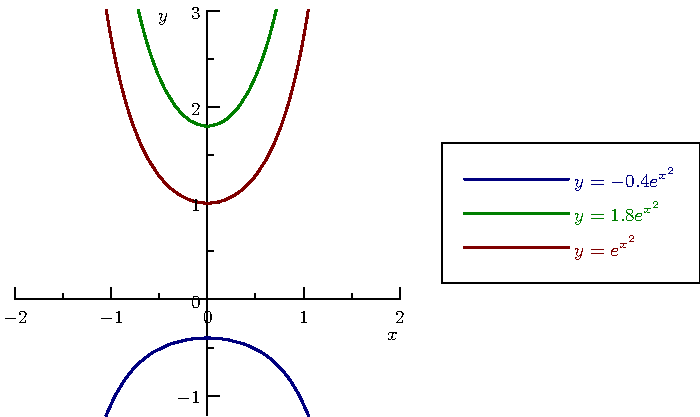
\includegraphics[width=\linewidth]{generated/asymptote/image-1.pdf}
\end{image}%
\tcblower
\end{figureptx}%
Solutions of ODEs that depend on arbitrary constants, such as \(y = Ce^{x^{2}}\) above, are called \terminology{general solutions}. Solutions of ODEs that do not depend on arbitrary constants, such as \(y = 5e^{x^{2}}\), are called \terminology{particular solutions}.%
\begin{example}{A trigonometric solution.}{x:example:example-a-trigonometric-sol}%
Show that \(x = A\cos(3t) + B\sin(3t)\), where \(A\) and \(B\) are arbitrary constants, is a general solution of \(x'' + 9x = 0\). Then find a particular solution.%
\par\smallskip%
\noindent\textbf{\blocktitlefont Solution}.\hypertarget{g:solution:idp105548778892832}{}\quad{}To check that \(x = A\cos(3t) + B\sin(3t)\) is a general solution of \(x''+9x = 0\), we just need to plug it into the ODE and show that it satisfies it. Since%
\begin{equation*}
x'' = -9(A\cos(3t)+B\sin(3t)) = -9x,
\end{equation*}
this follows very quickly.%
\par
To find a particular solution, all we need to do in this case is to pick specific values for \(A\) and \(B\) (any values will work here). So one particular solution of \(x''+9x = 0\) is given by \(x = \frac{3}{2}\cos(3t) - \sin(3t)\), among infinitely many others.%
\end{example}
In \hyperref[x:example:example-a-trigonometric-sol]{Example~{\xreffont\ref{x:example:example-a-trigonometric-sol}}}, to find a particular solution we just needed to plug in specific values for the arbitrary constants. In general, the particular solutions we'll be interested in are chosen to satisfy a given condition, which we call an \terminology{initial condition}. These conditions often take the form \(y(x_{0}) = y_{0}\). Geometrically, we are picking a specific point \((x_{0},y_{0})\) in the \(xy\)-plane that the solution must pass through.%
\par
An ODE together with an initial condition is called an \terminology{initial value problem (IVP)}. Although ODEs by themselves typically have infinitely many solutions, specifying an initial condition that the solution must satisfy is often enough to get a unique particular solution instead of a general solution.%
\begin{example}{Solving an IVP.}{x:example:example-solving-an-ivp}%
Solve the IVP \(\dv{y}{x} = -xe^{-x^{2}}, y(0)=1\).%
\par\smallskip%
\noindent\textbf{\blocktitlefont Solution}.\hypertarget{g:solution:idp105548778900640}{}\quad{}We need to find a function \(y\) that satisfies two different constraints: \(y' = -xe^{-x^{2}}\) and \(y(0)=1\). We'll start with the first one, which we actually know how to do from Calculus I. If \(y' = -xe^{-x^{2}}\), then%
\begin{equation*}
y = \int -xe^{-x^{2}}\,dx = \frac{1}{2}e^{-x^{2}}+C.
\end{equation*}
Now we need to make sure that \(y\) is equal to \(1\) if \(x=0\). We do this by setting \(y=1\), \(x=0\) and choosing the right value for \(C\) to make the resulting equation true:%
\begin{equation*}
1 = \frac{1}{2} + C \Rightarrow C = \frac{1}{2}.
\end{equation*}
So the solution of this IVP is the function \(y = \frac{e^{-x^{2}}+1}{2}\).%
\end{example}
Two important things to keep in mind before we move to the next topic:%
\begin{enumerate}
\item{}ODEs by themselves have general solutions, whereas IVPs have particular solutions.%
\item{}When solving IVPs, it's important to keep track of any arbitrary constants that appear. Neglecting arbitrary constants usually makes it impossible to find the right particular solution.%
\end{enumerate}
%
\end{subsectionptx}
%
%
\typeout{************************************************}
\typeout{Subsection  Mathematical Models}
\typeout{************************************************}
%
\begin{subsectionptx}{Mathematical Models}{}{Mathematical Models}{}{}{x:subsection:subsection-mathematical-models}
Differential equations are useful because they can provide a mathematical model of a physical quantity. Analyzing the model allows us to infer something meaningful about the quantity in question. A relatively simple model comes from \terminology{Newton's Law of Cooling}, which relates the temperature of an object with the temperature of the surrounding medium (such as air or water). In particular, Newton's Law of Cooling states that the time rate of change of the temperature of an object is proportional to the difference of the temperature of the object with that of the temperature of the surrounding medium.%
\begin{example}{Newton's Law of Cooling.}{x:example:example-newton-s-law-of-cooling}%
Restate Newton's Law of Cooling as a differential equation.%
\par\smallskip%
\noindent\textbf{\blocktitlefont Solution}.\hypertarget{g:solution:idp105548780155168}{}\quad{}It may not be obvious that Newton's Law of Cooling can be restated as a differential equation, but the phrase "rate of change" that appears in the statement of the law is a good clue that this can be done. To do this, first we need to give the relevant quantities (the temperature of the object and the temperature of the surrounding medium) names. Let \(T(t)\) denote the temperature of the object at time \(t\) and let \(A(t)\) denote the temperature of the surrounding medium at time \(t\). Then Newton's Law of Cooling says that%
\begin{equation*}
\dv{T}{t} = k(T-A)
\end{equation*}
where \(k\) is some constant.%
\par
Although we can't determine \(k\) precisely (this would require experimentation and depends on the object and medium in question), we can still say something useful about it. In particular, \(k\) must be negative. To see why, consider what the object does if \(T\gt A\) and \(T\lt A\). If \(T\gt A\), then the object must be cooling since the surrounding medium is cooler than the object. If the object is cooling, then \(\dv{T}{t}\lt0\). On the other hand, if \(T\lt A\) then \(\dv{T}{t}\gt0\) since the object would be heating up in this case. The only way for this to occur is if \(k\lt0\).%
\end{example}
Most of the mathematical models we'll look at will take the form of an IVP.%
\begin{example}{An IVP modeling a falling object.}{x:example:example-an-ivp-modeling-a-falling-object}%
A ball weighing \SI{0.5}{\kilo\gram} is dropped from a height of \SI{100}{\meter} and is acted upon by gravity and air resistance. Assuming that the force of air resistance is proportional to the velocity of the ball, what is an IVP that models the movement of the ball?%
\par\smallskip%
\noindent\textbf{\blocktitlefont Solution}.\hypertarget{g:solution:idp105548780164512}{}\quad{}What we need to do is to translate this physical situation into mathematics, and to do that we need to start assigning names to the quantities of interest. The quantities that matter in this problem are the movement of the ball, the force of gravity and the force of air resistance. We'll name them as follows:%
\begin{align*}
\text{height of the ball  seconds after its released} &= y(t) \\
\text{force of gravity} &= F_{G} = mg = -4.9\\
\text{force of air resistance} &= F_{R} = k\dv{y}{t} 
\end{align*}
where \(C\) is negative (since air resistance should act \emph{against} velocity). To get a differential equation out of all this, we'll use Newton's Second Law (which is actually a second-order ODE in disguise). This says that the net force on the ball should be equal to its mass times acceleration: \(F = ma\). So we have%
\begin{equation*}
F_{G}+F_{R} = 0.5\dv[2]{y}{t}
\end{equation*}
or just%
\begin{equation*}
-4.9+k\dv{y}{t} = 0.5\dv[2]{y}{t}.
\end{equation*}
The initial condition in this case would be \(y(0) = 100\). So our IVP is%
\begin{equation*}
-4.9+k\dv{y}{t} = 0.5\dv[2]{y}{t}, y(0) = 100.
\end{equation*}
%
\end{example}
One quick note about the IVP in \hyperref[x:example:example-an-ivp-modeling-a-falling-object]{Example~{\xreffont\ref{x:example:example-an-ivp-modeling-a-falling-object}}} The differential equation was second-order, but there was only one corresponding initial condition. As we'll see later, this is not enough to find a unique solution to this IVP. For most IVPs we'll solve, we'll need as many initial conditions as the order of the ODE. Something to look forward to.%
\end{subsectionptx}
\begin{conclusion}{}%
Now that we have a rough idea of what an ODE and an IVP actually are, we can move on to solving them. In the next section, we'll look at a method that we can use to visualize ODEs and their solutions and another method that can be used to approximate solutions of ODEs.%
\par
SUGGESTED PROBLEMS: 1-13 odd%
\end{conclusion}%
\end{sectionptx}
%
%
\typeout{************************************************}
\typeout{Section 1.2 Direction Fields}
\typeout{************************************************}
%
\begin{sectionptx}{Direction Fields}{}{Direction Fields}{}{}{x:section:section-direction-fields}
\begin{introduction}{}%
This section corresponds to Section 1.2 from the textbook.%
\end{introduction}%
%
%
\typeout{************************************************}
\typeout{Subsection  Direction Fields and Solution Curves}
\typeout{************************************************}
%
\begin{subsectionptx}{Direction Fields and Solution Curves}{}{Direction Fields and Solution Curves}{}{}{x:subsection:subsection-direction-fields-and-solution-curves}
Suppose we wanted to solve the ODE \(\dv{y}{x} = x\). Then we can do so using the tools already available to us, since the mystery function \(y=y(x)\) must have derivative given by \(x\). So%
\begin{equation*}
y = \int x\,dx = \frac{1}{2}x^{2}+C.
\end{equation*}
Any choice for \(C\) yields another solution of the ODE \(\dv{y}{x} = x\).%
\begin{aside}{}{g:aside:idp105548780175392}%
Again, it's very important in this course not to forget the arbitrary constant \(C\)!%
\end{aside}
Now let's make things a little more interesting. Suppose we wanted to solve the ODE \(\dv{y}{x} = e^{-x^{2}}\). Then this is \emph{impossible} to do in a single "closed-form". \begin{aside}{}{g:aside:idp105548780177312}%
By closed-form we basically mean in terms of the usual exponential, trigonometric and polynomial functions, as well as their inverses.%
\end{aside}
 This is because solving this ODE requires integrating \(e^{-x^{2}}\), which as you may remember from Calculus 2 cannot be done without resorting to something like power series. Even if we can't solve the ODE, or if we can't solve it easily, we still want to be able to obtain some information from it. One way to do this is by using \terminology{direction fields}, which is a graphical representation of the ODE.%
\par
To construct a direction field for an ODE of the form%
\begin{equation*}
\dv{y}{x} = f(x,y)
\end{equation*}
perform the following steps:%
\begin{enumerate}
\item{}Pick a point \((a,b)\) in the \(xy\)-plane.%
\item{}Plug the point \((a,b)\) into \(f(x,y)\) to obtain the number \(f(a,b)\).%
\item{}Plot a short line segment with slope \(f(a,b)\) at the point \((a,b)\).%
\item{}Repeat at several other points in the \(xy\)-plane until you develop a satisfactory picture of the behavior of the ODE.%
\end{enumerate}
The resulting graph is called the direction field for the ODE.%
\begin{aside}{}{g:aside:idp105548780183584}%
Direction fields are often called slope fields.%
\end{aside}
\begin{example}{Plotting a direction field by hand.}{x:example:example-plotting-a-direction-field-by-hand}%
Fill in the direction field for \(y' = t - y\) at the indicated points:%
\begin{figureptx}{}{x:figure:figure-dirfield-template}{}%
\begin{image}{0.25}{0.5}{0.25}%
\resizebox{\linewidth}{!}{%
    \begin{tikzpicture}
    \begin{axis}[%
    axis x line = center,
    axis y line = center,
    grid=both,
    xtick={-1,...,3},
    ytick={-1,...,3},
    xmin=-2,
    xmax=4,
    ymin=-2,
    ymax=4,
    xlabel={$t$},
    ylabel={$y$}
    ]
    \addplot[only marks,mark=*] table[row sep=\\]{%
    1   1\\
    0   2\\
    2   2\\
    2   1\\
    0   0\\
    0   1\\
    0   2\\
    1   2\\
    1   0\\
    2   0\\
    };
    \end{axis}
\end{tikzpicture}
}%
\end{image}%
\tcblower
\end{figureptx}%
\par\smallskip%
\noindent\textbf{\blocktitlefont Solution}.\hypertarget{g:solution:idp105548780119968}{}\quad{}To plot the direction field, remember that we're basically plotting \emph{slopes}. So we first need to figure out \(y' = t-y\) at the indicated points. The following table lists values for \(y'\) at some of these points: \begin{tableptx}{\textbf{}}{g:table:idp105548780121504}{}%
\centering%
{\tabularfont%
\begin{tabular}{cc}\hrulethick
\((t,y)\)&\(y' = t-y\)\tabularnewline\hrulethin
\((0,0)\)&\(0-0 = 0\)\tabularnewline\hrulethin
\((2,2)\)&\(2-2=0\)\tabularnewline\hrulethin
\((1,2)\)&\(1-2 = -1\)\tabularnewline\hrulethin
\((0,1)\)&\(0-1=-1\)\tabularnewline\hrulethick
\end{tabular}
}%
\end{tableptx}%
 If we fill out the remaining values of \(y'\) and plot the corresponding slopes, we should get something like this:%
\begin{figureptx}{}{g:figure:idp105548780127520}{}%
\begin{image}{0.25}{0.5}{0.25}%
\resizebox{\linewidth}{!}{%
\def\length{sqrt(1+(x-y)^2)}
\begin{tikzpicture}
\begin{axis}[
    axis x line = center,
    axis y line = center,
    grid=both,
    xlabel={$t$},
    ylabel={$y$},
    view={0}{90},
    domain=0:2,
    y domain=0:2,
    xmin=-2, ymin=-2,
    xmax=4, ymax=4,
    xtick={-1,...,3},
    ytick={-1,...,3},
    samples=3
]
\addplot3 [blue, thick, quiver={u={1/(\length)}, v={(x-y)/(\length)}, scale arrows=0.5}] {0};
\addplot[only marks,mark=*] table[row sep=\\]{%
1   1\\
0   2\\
2   2\\
2   1\\
0   0\\
0   1\\
0   2\\
1   2\\
1   0\\
2   0\\
};
\end{axis}
\end{tikzpicture}
}%
\end{image}%
\tcblower
\end{figureptx}%
\end{example}
\begin{example}{Plotting a direction field with a CAS.}{x:example:example-plotting-a-direction-field-with-a-cas}%
Plot the direction field for the differential equation \(x' = x(1-x)\), where \(x=x(t)\).%
\par\smallskip%
\noindent\textbf{\blocktitlefont Solution}.\hypertarget{g:solution:idp105548780129824}{}\quad{}We can easily do this with a computer system (such as Sage!). For example, try running the cell below this example. If we do so, we get something like the following diagram:%
\begin{figureptx}{The direction field for \(x' = x(1-x)\).}{x:figure:figure-dirfield1}{}%
\begin{image}{0.25}{0.5}{0.25}%
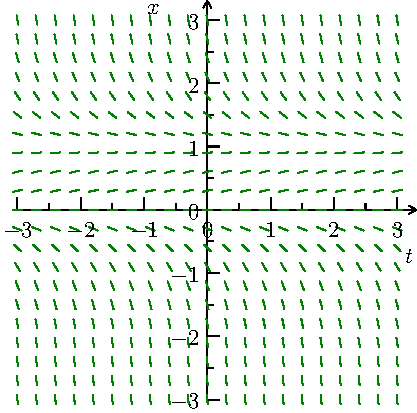
\includegraphics[width=\linewidth]{generated/asymptote/image-4.pdf}
\end{image}%
\tcblower
\end{figureptx}%
\end{example}
\begin{sageinput}
var('t, x')    # tells Sage what variables we're using
f = x * (1 - x)
plot_slope_field(f, (t, -10, 10), (x, -5, 5), color = "blue")
\end{sageinput}
Direction fields are useful because they provide a means to obtain information about a differential equation (and the corresponding model) without actually having to solve the differential equation. One way to do so is to create a \emph{streamline plot}. This can be done easily in Sage, like so: \begin{sageinput}
var('t, x')
f = x * (1 - x)
streamline_plot(f, (t, -5, 5), (x, -1, 2))
\end{sageinput}
 This can also be created by hand from a slope field without too much trouble.%
\par
If we only graph a single curve in the direction field we get what's known as a \terminology{solution curve}, which represents a solution of an initial value problem corresponding to the ODE the direction field is drawn from.%
\begin{example}{Information from a solution curve.}{x:example:example-information-from-a-solution-curve}%
Let \(x(t)\) represent the solution of the initial value problem%
\begin{align*}
x' & = x(1-x) \\
x(0) & = \frac{1}{2}. 
\end{align*}
Determine \(\lim_{t\to\infty}x(t)\).%
\par\smallskip%
\noindent\textbf{\blocktitlefont Solution}.\hypertarget{g:solution:idp105548780136224}{}\quad{}Since we don't know how to solve this IVP yet, we'll make use of the direction field from \hyperref[x:example:example-plotting-a-direction-field-with-a-cas]{Example~{\xreffont\ref{x:example:example-plotting-a-direction-field-with-a-cas}}} to find an approximate solution curve. Since the initial condition is \(x(0) = \frac{1}{2}\), this means that the solution must pass through the point \((0,\frac{1}{2})\). So if we start at this point and trace a curve that flows with the direction field, we get the following solution curve:%
\begin{figureptx}{The solution curve corresponding to the initial condition \(x(0) = \frac{1}{2}\).}{x:figure:figure-solcurve1}{}%
\begin{image}{0.25}{0.5}{0.25}%
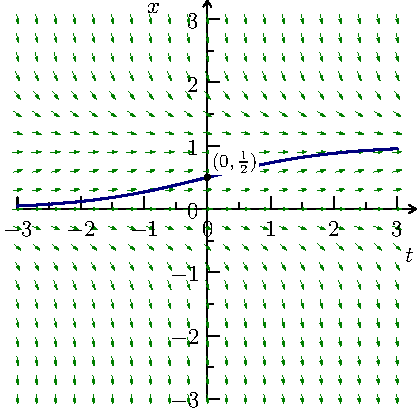
\includegraphics[width=\linewidth]{generated/asymptote/image-5.pdf}
\end{image}%
\tcblower
\end{figureptx}%
So it appears that \(\lim_{t\to\infty}x(t) = 1\).%
\end{example}
\end{subsectionptx}
\begin{conclusion}{}%
SUGGESTED PROBLEMS: 1-7 odd%
\end{conclusion}%
\end{sectionptx}
%
%
\typeout{************************************************}
\typeout{Section 1.3 Separable ODEs and Substitution}
\typeout{************************************************}
%
\begin{sectionptx}{Separable ODEs and Substitution}{}{Separable ODEs and Substitution}{}{}{x:section:section-separable-odes-and-substitution}
\begin{introduction}{}%
This section corresponds to Section 1.3 from the text.%
\end{introduction}%
%
%
\typeout{************************************************}
\typeout{Subsection  Separable ODEs}
\typeout{************************************************}
%
\begin{subsectionptx}{Separable ODEs}{}{Separable ODEs}{}{}{x:subsection:subsection-separable-odes}
The simplest ODEs to solve are the first-order ODEs of the form \(\dv{y}{x} = f(x)\). The Fundamental Theorem of Calculus guarantees that the solution \(y\) is given by \(y = \int f(x)\,dx\).%
\begin{aside}{}{g:aside:idp105548780144544}%
\end{aside}
Another type of ODE that is relatively straightforward to solve is the \terminology{separable ODE}, which is a first-order ODE that can be written in the form%
%
\begin{equation*}
\dv{y}{x} = f(x)g(y).
\end{equation*}
These ODEs can be solved by integration as well, but only after some rearranging.%
\begin{example}{Solving a separable ODE.}{x:example:example-solving-a-separable-ode}%
Solve the IVP given by \(y' = x+4xy^{2}, y(0)=1\).%
\par\smallskip%
\noindent\textbf{\blocktitlefont Solution}.\hypertarget{g:solution:idp105548780148000}{}\quad{}The first step to solving this IVP is to solve the ODE \(y' = x+4xy^{2}\). It may not look like it at first, but this ODE is separable since we can rewrite it as \(y' = x(1+4y^{2})\). To solve this ODE, we need to move the \(y\) terms to the left hand side of the equation and the \(x\) terms to the right hand side. We'll abuse notation a little bit to do so by rewriting \(y' = \dv{y}{x}\) and treating \(\dv{y}{x}\) as a fraction, but it won't get us into too much trouble here:%
%
\begin{align*}
\dv{y}{x} = x(1+4y^{2}) &\Rightarrow \frac{dy}{1+4y^{2}} = x\,dx \\
&\Rightarrow \int\frac{dy}{1+4y^{2}}  = \int x\,dx \\
&\Rightarrow \frac{1}{2}\tan^{-1}(2y)  = \frac{1}{2}x^{2}+C \\
&\Rightarrow \tan^{-1}(2y)  = x^{2}+C_{1} 
\end{align*}
At this step we can either leave the solution as is (in \terminology{implicit form}) or solve for \(y\) to get an \terminology{explicit form}. We'll leave this in implicit form and then plug in the initial condition to get%
\begin{equation*}
\tan^{-1}(2) = C_{1}.
\end{equation*}
So the implicit solution of this IVP is given by%
\begin{equation*}
\tan^{-1}(2y) = x^{2}+\tan^{-1}(2).
\end{equation*}
%
\end{example}
\begin{example}{Newton's Law of Cooling again.}{x:example:example-newton-s-law-of-cooling-again}%
A metal plate is removed from an oven and placed in a room. The temperature of the plate is \(100^{\circ}\) Celsius and the temperature of the room is fixed at \(15^{\circ}\) Celsius. After \(20\) minutes the temperature of the plate drops to \(90^{\circ}\) Celsius. How hot is the plate after five hours?%
\par\smallskip%
\noindent\textbf{\blocktitlefont Solution}.\hypertarget{g:solution:idp105548780090528}{}\quad{}Let \(T(t)\) denote the temperature of the plate \(t\) minutes after being removed from the oven and let \(A(t)\) denote the temperature of the room \(t\) minutes after the plate is removed from the oven. Then \(T(0) = 100\) and Newton's Law of Cooling says that%
%
\begin{equation*}
\dv{T}{t} = k(T-15).
\end{equation*}
To answer this question we need to find \(T\), and although we don't know \(k\) at the moment we can still make some progress just by remembering that it's a constant. This ODE is separable, so we'll separate variables and integrate both sides to get%
\begin{equation*}
\ln(T-15) = kt+C
\end{equation*}
which simplifies to \(T-15 = C_{1}e^{kt}\) or just \(T = 15+C_{1}e^{kt}\).%
\par
Now we need to find \(C_{1}\) and \(k\). To find \(C_{1}\), we just use the initial condition to get \(C_{1} = 85\). The only piece of information that we have left to find \(k\) is the fact that the temperature of the plate drops to \(90\) after \(20\) minutes. In other words, \(T(20) = 90\). Therefore%
\begin{equation*}
90 = 15+85e^{20k}
\end{equation*}
which becomes%
\begin{equation*}
\ln\frac{75}{85} = 20k\text{.}
\end{equation*}
Therefore \(k = \frac{1}{20}\ln\frac{15}{17}\approx-.006.\)%
\par
So, finally, \(T(t) = 15+85e^{-.006t}\) and the temperature after five hours is \(T(300)\approx28\).%
\end{example}
\end{subsectionptx}
%
%
\typeout{************************************************}
\typeout{Subsection  Substitution Methods}
\typeout{************************************************}
%
\begin{subsectionptx}{Substitution Methods}{}{Substitution Methods}{}{}{x:subsection:subsection-substitution-methods}
At this point we can only solve a couple types of differential equations. An ODE that isn't of the form \(\dv{y}{x} = f(x)\) or separable may prove troublesome. However, there are certain cases where we can rewrite an ODE into one of these forms by using the right substitution.%
\begin{example}{Substitution to solve an ODE.}{x:example:example-substitution-to-solve-an-ode}%
Find the general solution of \(y' = (x+y+3)^{2}\).%
\par\smallskip%
\noindent\textbf{\blocktitlefont Solution}.\hypertarget{g:solution:idp105548780103584}{}\quad{}This ODE is not separable and we can't just integrate it (since the right hand side depends on the dependent variable). However, the form of the right hand side suggests a substitution: \(u = x+y+3\). This would simplify things quite a bit, leaving us with \(y'=u^{2}\). The only problem with this is that \(y'\) depends on \(x\), not \(u\). We must rewrite \(y'\) in terms of the new variable \(u\), which isn't too bad. Since \(u = x+y+3\), we get \(y' = u'-1\). Therefore the ODE becomes%
\begin{equation*}
u'-1 = u^{2}\text{ or just }\dv{u}{x} = 1+u^{2}.
\end{equation*}
%
\par
This new ODE \emph{is} separable, and so we separate variables and integrate to get \(\tan^{-1}u = x+C\). If we don't care about finding an explicit solution, then we can just replace \(u\) to get the equation back in terms of \(y\). So our (implicit) general solution is \(\tan^{-1}(x+y+3) = x+C\).%
\end{example}
\begin{example}{A less obvious substitution.}{x:example:example-a-less-obvious-substitution}%
Find an explicit solution of \(xy'=x+y\).%
\par\smallskip%
\noindent\textbf{\blocktitlefont Solution}.\hypertarget{g:solution:idp105548780111264}{}\quad{}It's tough to see what to do right away, so we'll try simplifying the ODE first. In particular, we'll solve for \(y'\) to get%
\begin{equation*}
y' = 1+\frac{y}{x}.
\end{equation*}
If we stare at this for a while, we might convince ourselves that the right hand side really just depends on \(\frac{y}{x}\), so we'll try replacing that with \(u\). Then the ODE becomes \(y'=1+u\).%
\par
Once again, this is much simpler but we need to rewrite \(y'\) in terms of \(u\). Since \(u=\frac{y}{x}\), this means that \(y=ux\) and so \(y' = u+u'x\). Then the ODE becomes%
\begin{equation*}
u+x\dv{u}{x} = 1+u\text{ or just } x\dv{u}{x} = 1\text{.}
\end{equation*}
%
\par
This new ODE can be rearranged to get \(\dv{u}{x} = \frac{1}{x}\), and so \(u = \ln|x|+C\). Getting back in terms of \(y\), we have \(\frac{y}{x} = \ln|x|+C\) or just \(y = x\ln|x|+Cx\).%
\end{example}
\end{subsectionptx}
\begin{conclusion}{}%
SUGGESTED PROBLEMS: 3, 5, 9, 11, 15, 19, 25%
\end{conclusion}%
\end{sectionptx}
%
%
\typeout{************************************************}
\typeout{Section 1.4 First-Order Linear ODEs}
\typeout{************************************************}
%
\begin{sectionptx}{First-Order Linear ODEs}{}{First-Order Linear ODEs}{}{}{x:section:section-first-order-linear-odes}
\begin{introduction}{}%
In this section we introduce a new type of ODE that we can solve, in addition to separable ODEs and "simple" ODEs of the form \(y'=f(x)\). The ODEs that we'll consider in this section are \terminology{first-order linear ODEs}.%
\begin{definition}{First-Order Linear ODEs.}{x:definition:definition-first-order-linear-odes}%
\index{first-order ODEs!first-order linear ODEs}%
A first-order ODE is said to be linear if it can be written in the following form:%
\begin{equation*}
\dv{y}{x} + P(x)y = Q(x).
\end{equation*}
%
\end{definition}
We've actually seen such an ODE all the way back in \hyperref[x:example:example-an-ivp-modeling-a-falling-object]{Example~{\xreffont\ref{x:example:example-an-ivp-modeling-a-falling-object}}}. The ODE that we came up with in that problem can be rewritten as a first-order linear ODE with the right substitution (say, \(u = y'\)). Our first goal in this section is then to figure out how to solve these ODEs.%
\par
Note that this section corresponds to Section 1.5 from the text.%
\end{introduction}%
%
%
\typeout{************************************************}
\typeout{Subsection  Integrating Factors}
\typeout{************************************************}
%
\begin{subsectionptx}{Integrating Factors}{}{Integrating Factors}{}{}{x:subsection:subsection-integrating-factors}
To get a sense of how to solve first-order linear ODEs, we'll try some relatively simple examples first.%
\begin{example}{Solving a first-order linear ODE.}{x:example:example-solving-a-first-order-linear-ode}%
Find the general solution of \(\dv{y}{x}+2y = x\).%
\par\smallskip%
\noindent\textbf{\blocktitlefont Solution}.\hypertarget{g:solution:idp105548780060960}{}\quad{}First, note that the ODE is indeed a first-order linear ODE since it takes the form given in \hyperref[x:definition:definition-first-order-linear-odes]{Definition~{\xreffont\ref{x:definition:definition-first-order-linear-odes}}}. If we stare at the ODE for a bit, we might think that the left hand side looks like something we'd get after using the product rule. Just compare \((fg)' = fg'+f'g\) with \(\dv{y}{x}+2y\), and it appears that the unknown function \(y\) is taking the place of \(g\) in the product rule formula. If we could just figure out what the function \(f\) is supposed to be, then we could drastically simplify the left hand side of the ODE.%
\par
Unfortunately, there is no such function \(f\) that works here. If there were, we'd have to have \(f'=2\) and \(f=2x\), and clearly we aren't multiplying \(\dv{y}{x}\) by \(2x\) in the ODE. But we can pull a dirty trick here! We'll multiply through the ODE by \(e^{2x}\) to get the new ODE%
\begin{equation*}
e^{2x}\dv{y}{x}+2e^{2x}y = xe^{2x}.
\end{equation*}
It might not be all that obvious why this helps us out, but now the left hand side can be simplified by the product rule:%
\begin{equation*}
e^{2x}\dv{y}{x}+2e^{2x}y = \dv{}{x}[e^{2x}y].
\end{equation*}
%
\par
So we can rewrite the entire ODE as%
\begin{equation*}
\dv{}{x}[e^{2x}y] = xe^{2x}.
\end{equation*}
We can integrate this on both sides to get \(e^{2x}y = \int xe^{2x}\,dx\), or just%
\begin{equation*}
e^{2x}y = \frac{1}{2}xe^{2x} - \frac{1}{4}e^{2x}+C.
\end{equation*}
The explicit solution would be \(y = \frac{1}{2}x - \frac{1}{4} + Ce^{-2x}\).%
\end{example}
The function \(e^{2x}\) that we used in \hyperref[x:example:example-solving-a-first-order-linear-ode]{Example~{\xreffont\ref{x:example:example-solving-a-first-order-linear-ode}}} is called an \terminology{integrating factor}. Integrating factors are our primary tool in solving first-order linear ODEs. In general, to solve a first-order linear ODE \(y' +P(x)y=Q(x)\) the first thing you must do is to multiply through it by the integrating factor \(e^{\int P(x)\,dx}\).%
\begin{example}{Solving a first-order linear ODE in disguise.}{x:example:example-solving-a-first-order-linear-ode-in-disguise}%
Solve the second-order ODE given by%
\begin{equation*}
tx''+\frac{t}{1+t^{2}}x' = \frac{2t^{2}}{(1+t^{2})^{2}}e^{-\tan^{-1}t}
\end{equation*}
with initial conditions \(x(0) = x'(0) = -1.\)%
\par\smallskip%
\noindent\textbf{\blocktitlefont Solution}.\hypertarget{g:solution:idp105548780072992}{}\quad{}Even though this is a second-order ODE, we can rewrite it as a first-order ODE using the substitution \(u = x'\). Then the ODE becomes%
\begin{equation*}
tu+\frac{t}{1+t^{2}}u = \frac{2t^{2}}{(1+t^{2})^{2}}e^{-\tan^{-1}t}.
\end{equation*}
If we divide through by \(t\), we get%
\begin{equation*}
u+\frac{1}{1+t^{2}}u = \frac{2t}{(1+t^{2})^{2}}e^{-\tan^{-1}t}.
\end{equation*}
This can be solved by integrating factors since it takes the form given in \hyperref[x:definition:definition-first-order-linear-odes]{Definition~{\xreffont\ref{x:definition:definition-first-order-linear-odes}}}. The integrating factor we need is given by%
\begin{equation*}
e^{\int \frac{1}{1+t^{2}}\,dt} = e^{\tan^{-1}t}.
\end{equation*}
%
\par
Now we multiply through the ODE by this integrating factor and rewrite the left hand side using the product rule to get%
\begin{equation*}
\dv{}{t}[e^{\tan^{-1}t}u] = \frac{2t}{(1+t^{2})^{2}}.
\end{equation*}
At this step we can integrate both sides to get%
\begin{equation*}
e^{\tan^{-1}t}u = -\frac{1}{1+t^{2}}+C,
\end{equation*}
which becomes%
\begin{equation*}
x' = -\frac{e^{-\tan^{-1}t}}{1+t^{2}}+Ce^{-\tan^{-1}t}.
\end{equation*}
%
\par
If we plug in the initial condition \(x'(0) = -1\), this forces \(C=0\). Hence%
\begin{equation*}
x' = -\frac{e^{-\tan^{-1}t}}{1+t^{2}}.
\end{equation*}
Now we integrate one last time to get \(x\):%
\begin{equation*}
x = e^{-\tan^{-1}t}+D.
\end{equation*}
If we use the last initial condition \(x(0)=-1\), we see that \(D = -2\). Hence the solution of this IVP is%
\begin{equation*}
x = e^{-\tan^{-1}t}-2.
\end{equation*}
%
\end{example}
\end{subsectionptx}
%
%
\typeout{************************************************}
\typeout{Subsection  Applications}
\typeout{************************************************}
%
\begin{subsectionptx}{Applications}{}{Applications}{}{}{x:subsection:subsection-applications}
A common application of first-order linear ODEs is in modeling "mixture" problems. Suppose we have a tank which contains a solution (mixture of solute and solvent, such as salt and water). Some amount of solution is also flowing into and out of the tank. We want to measure the amount of solute in the tank at time \(t\), call this amount \(x(t)\). Then \(x(t)\) will change depending on how the solute flows into and out of the tank, making it a prime target for a differential equation.%
\par
If we set%
\begin{align*}
c_{i} & =\text{concentration of solute flowing in} \\
c_{o} & =\text{concentration of solute flowing out} \\
r_{i} & =\text{rate solution is flowing in} \\
r_{o} & = \text{rate solution is flowing out} 
\end{align*}
then we can say that%
\begin{equation*}
\dv{x}{t} = r_{i}c_{i} - r_{o}c_{o} = r_{i}c_{i} - r_{0}\frac{x(t)}{V(t)}
\end{equation*}
where \(V(t)\) is the volume of solution in the tank at time \(t\). \begin{aside}{}{g:aside:idp105548780282272}%
We assume that \(c_{i},r_{i},r_{o}\) are all constant.%
\end{aside}
 Furthermore, if we let \(V_{0} = V(0)\) denote the initial volume of the solution in the tank then we can say that \(V(t) = V_{0} + (r_{i}-r_{0})t.\) Hence the amount of solute \(x(t)\) obeys the first-order linear ODE%
\begin{equation*}
\dv{x}{t} = r_{i}c_{i} - \frac{r_{o}}{V_{0}+(r_{i}-r_{o})t}x.
\end{equation*}
%
\begin{example}{Salt in a tank.}{x:example:example-salt-in-a-tank}%
A tank contains \SI{100}{\liter} of a solution consisting of \SI{50}{\kilo\gram} of salt dissolved in water. Solution containing \SI{1}{\kilo\gram\per\liter} of salt is pumped into the tank at a rate of \SI{2}{\liter\per\minute} and the well-mixed solution is pumped out at the rate of \SI{3}{\liter\per\minute}. How much salt will be in the tank after \(t\) minutes?%
\par\smallskip%
\noindent\textbf{\blocktitlefont Solution}.\hypertarget{g:solution:idp105548780290848}{}\quad{}Let \(x(t)\) denote the amount of salt in the tank after \(t\) minutes, so \(x(0) = 50\). Then%
\begin{equation*}
\dv{x}{t} = r_{i}c_{i}-r_{o}c_{o} = 2\cdot1-3\frac{x}{100-t}.
\end{equation*}
We can rearrange this to get%
\begin{equation*}
\dv{x}{t} + \frac{3}{100-t}x = 2.
\end{equation*}
This ODE is linear and has integrating factor \((100-t)^{-3}\). Multiplying through the ODE by the integrating factor and rewriting it using the product rule then gives us%
\begin{equation*}
\dv{}{t}[(100-t)^{-3}x] = 2(100-t)^{-3}.
\end{equation*}
%
\par
Now we can integrate both sides to get%
\begin{equation*}
(100-t)^{-3}x = (100-t)^{-2}+C
\end{equation*}
or just \(x = 100-t+C(100-t)^{3}\). Finally, the initial condition can be used to show that \(C = -\frac{1}{20000}\), so \(x = 100-t - \frac{1}{20000}(100-t)^{3}\).%
\end{example}
\end{subsectionptx}
\begin{conclusion}{}%
SUGGESTED PROBLEMS: 3-11 odd, 31, 33.%
\end{conclusion}%
\end{sectionptx}
%
%
\typeout{************************************************}
\typeout{Section 1.5 Existence and Uniqueness of Solutions}
\typeout{************************************************}
%
\begin{sectionptx}{Existence and Uniqueness of Solutions}{}{Existence and Uniqueness of Solutions}{}{}{x:section:section-existence-and-uniqueness-of-solutions}
\begin{introduction}{}%
This section corresponds to Section 1.7 from the text.%
\end{introduction}%
%
%
\typeout{************************************************}
\typeout{Subsection  Existence and Uniqueness Theorem}
\typeout{************************************************}
%
\begin{subsectionptx}{Existence and Uniqueness Theorem}{}{Existence and Uniqueness Theorem}{}{}{x:subsection:subsection-existence-and-uniqueness-theorem}
There are two important questions we need to consider when developing a mathematical model using differential equations (i.e. IVPs):%
\begin{enumerate}
\item{}Does the initial value problem have a solution? (Existence).%
\item{}If it has a solution, is the solution unique? (Uniqueness).%
\end{enumerate}
Ideally, the answer to both of these questions will be yes.%
\begin{example}{The answer is no.}{x:example:example-the-answer-is-no}%
Does \(x\dv{y}{x} = \sqrt[3]{y},y(1) = 0\) have a unique solution?%
\par\smallskip%
\noindent\textbf{\blocktitlefont Solution}.\hypertarget{g:solution:idp105548780300576}{}\quad{}We can find a solution to this IVP by treating the ODE as separable. If we do so, we find that \(y = \left(\frac{2}{3}\ln x\right)^{\frac{3}{2}}\). On the other hand, we can also eyeball a second solution: \(y=0\). So this IVP has \emph{two} different solutions: \(y_{1} = \left(\frac{2}{3}\ln x\right)^{\frac{3}{2}}\) and \(y_{2} = 0\).%
\end{example}
Clearly, IVPs don't always have unique solutions. Sometimes it's difficult to determine precisely when an IVP can have a unique solution, but most of the cases we'll care about in this class will fall under the following theorem.%
\begin{theorem}{Existence and Uniqueness Theorem.}{}{x:theorem:theorem-existence-and-uniqueness-theorem}%
\index{first-order ODEs!existence and uniqueness}%
Consider the IVP given by \(\dv{y}{x} = f(x,y), y(x_{0}) = y_{0}\). If \(f(x,y)\) is bounded and continuous within some rectangle in the plane containing \((x_{0},y_{0})\), then the IVP has at least one solution. If in addition \(f_{y}(x,y)\) is also bounded and continuous within some rectangle containing \((x_{0},y_{0})\), then the IVP has a unique solution.%
\end{theorem}
If we go back to \hyperref[x:example:example-the-answer-is-no]{Example~{\xreffont\ref{x:example:example-the-answer-is-no}}}, then we see that \hyperref[x:theorem:theorem-existence-and-uniqueness-theorem]{Theorem~{\xreffont\ref{x:theorem:theorem-existence-and-uniqueness-theorem}}} has something to say about the IVP in that example. In that example, we had \(f(x,y) = \sqrt[3]{y}, f_{y}(x,y) = \frac{1}{3}y^{-\frac{2}{3}}\) and \((x_{0},y_{0}) = (1,0)\). Let's draw a rectangle around this point: \begin{figureptx}{}{x:figure:figure-existence-and-uniqueness-1}{}%
\begin{image}{0.25}{0.5}{0.25}%
\resizebox{\linewidth}{!}{%
\begin{tikzpicture}
    \begin{axis}[%
    axis x line = center,
    axis y line = center,
    xlabel = {$x$},
    ylabel = {$y$},
    xmin=0,
    xmax=2,
    ymin=-1,
    ymax=2,
    grid = both
    ]
    \draw[fill=blue!40,opacity=.5] (.5,-.5) rectangle (1.5,1.5);
    \draw (1,1) node{$R$};
    \addplot[mark=*]table[row sep=\\]{%
    1   0\\
    } node[above right]{$(x_{0},y_{0})$};
    \end{axis}
\end{tikzpicture}
}%
\end{image}%
\tcblower
\end{figureptx}%
%
\par
Now \(f\) is continuous and \(-\frac{1}{2}\leq y\leq\frac{3}{2}\) within this rectangle, so%
\begin{equation*}
-\sqrt[3]{\frac{1}{2}}\leq f(x,y)\leq\sqrt[3]{\frac{3}{2}}
\end{equation*}
everywhere inside of this triangle. So \hyperref[x:theorem:theorem-existence-and-uniqueness-theorem]{Theorem~{\xreffont\ref{x:theorem:theorem-existence-and-uniqueness-theorem}}} guarantees \emph{at least one} solution of the IVP, and indeed there is at least one solution. However, the problem with uniqueness stems from the fact that \(f_{y}\) has a divide-by-zero problem inside this rectangle. Furthermore, it's impossible to draw a rectangle around \((1,0)\) that avoids this divide-by-zero problem. Hence there is no guarantee of uniqueness.%
\par
On the other hand, if we changed the initial condition to \(y(1) = 0.000001\) then we would be guaranteed a unique solution. Moving that initial condition off of the \(x\)-axis is all we need to do to guarantee uniqueness.%
\end{subsectionptx}
%
%
\typeout{************************************************}
\typeout{Subsection  Picard Iteration}
\typeout{************************************************}
%
\begin{subsectionptx}{Picard Iteration}{}{Picard Iteration}{}{}{x:subsection:subsection-picard-iteration}
Now that we know of a way to determine whether or not certain ODEs have solutions, we'd like a method for actually finding these solutions. We've seen a few different methods for solving specific first-order ODEs, but what we'll do now is discuss a method that works for a large class of first-order ODEs. The only catch is that it may take us an infinite amount of time to get the solution.%
\par
Consider the IVP \(\dv{y}{x} = f(x,y), y(x_{0}) = y_{0}\). We can rewrite this differential equation as an \terminology{integral equation}:%
\begin{equation*}
y(x) = y_{0} + \int_{x_{0}}^{x}f(t,y(t))\,dt.
\end{equation*}
It looks quite a bit different, but solutions of this integral equation are also solutions of the corresponding differential equation. Our goal now is to approximate a solution to this integral equation.%
\par
To start, let's make a guess as to what the solution of our IVP should be. To keep things simple we'll start with a constant function, say \(\phi_{0}(x) = y_{0}\) so that we at least satisfy the initial condition. Now this guess may not be a good match for the solution of the IVP away from the initial condition, so we'll adjust the guess using the integral equation to get the new function \(\phi_{1}\):%
\begin{equation*}
\phi_{1}(x) = y_{0} + \int_{x_{0}}^{x}f(t,\phi_{0})\,dt.
\end{equation*}
Now \(\phi_{1}\) may not be a great approximation either away from the initial condition, but we can adjust it using the integral equation just like we did to \(\phi_{0}\).%
\par
The method described in the previous paragraph is \terminology{Picard's Method}. In general, the \(n^{\text{th}}\) iteration of Picard's Method is given by%
\begin{equation*}
\phi_{n}(x) = y_{0}+\int_{x_{0}}^{x}f(t,\phi_{n-1}(t))\,dt,
\end{equation*}
and the first iterate is the constant function \(\phi_{0} = y_{0}.\) It may seem strange to consider these functions as approximate solutions of the IVP in question, but each iterate actually solves an IVP very similar to the one that we care about, \(\dv{y}{x} = f(x,y), y(x_{0}) = y_{0}\). In particular,%
\begin{equation*}
\dv{\phi_{n}}{x} = f(x,\phi_{n-1}), \phi_{n}(x_{0}) = y_{0}
\end{equation*}
for all \(n\geq1\). This method doesn't always work, but if \(f(x,y)\) satisfies the conditions given in \hyperref[x:theorem:theorem-existence-and-uniqueness-theorem]{Theorem~{\xreffont\ref{x:theorem:theorem-existence-and-uniqueness-theorem}}} then this method will (after potentially infinitely many steps) provide a solution to the IVP.%
\end{subsectionptx}
\end{sectionptx}
%
%
\typeout{************************************************}
\typeout{Section 1.6 Population Models and Autonomous Equations}
\typeout{************************************************}
%
\begin{sectionptx}{Population Models and Autonomous Equations}{}{Population Models and Autonomous Equations}{}{}{x:section:section-population-models-and-autonomous-equations}
%
%
\typeout{************************************************}
\typeout{Subsection  Population Equations}
\typeout{************************************************}
%
\begin{subsectionptx}{Population Equations}{}{Population Equations}{}{}{x:subsection:subsection-population-equations}
Suppose we're monitoring the population of some species, and let's denote the population at time \(t\) by \(P(t)\). An obvious question to consider is how that population will change over time. Mathematically, this means we want to obtain information on \(\dv{P}{t}\) and then use it to estimate \(P(t)\).%
\par
A simple model for \(\dv{P}{t}\) is to assume it depends only on the birth rate \(\beta\) and death rate \(\delta\) of the species in question. Then we can write%
\begin{equation}
\dv{P}{t} = (\beta - \delta)P.\label{x:men:equation-natural-growth}
\end{equation}
If we assume that \(\beta,\delta\) are constants, then this equation is separable and we can solve it to obtain%
\begin{equation*}
P(t) = P_{0}e^{(\beta - \delta)t},
\end{equation*}
where \(P_{0}\) represents the "initial population", or population at time \(t = 0\). We call \hyperref[x:men:equation-natural-growth]{({\xreffont\ref{x:men:equation-natural-growth}})} the \terminology{natural growth equation}.%
\par
The natural growth equation is simple, but it's probably too simple to be useful expect in certain scenarios (such as measuring half-life). To get a more flexible model, we can generalize \hyperref[x:men:equation-natural-growth]{({\xreffont\ref{x:men:equation-natural-growth}})} by assuming that the birth and death rates are actually functions of time. This gives us the \terminology{general population equation}.%
\begin{definition}{General Population Equation.}{x:definition:definition-general-population-equation}%
The general population equation for a population \(P(t)\) is given by%
\begin{equation*}
\dv{P}{t} = (\beta(t) - \delta(t))P.
\end{equation*}
%
\end{definition}
\begin{example}{Population Explosion.}{x:example:example-population-explosion}%
A population has \(100\) members at time \(t = 0\) years with a death rate of \(.25P\) and a birth rate of \(.5P\), where \(P(t)\) denotes the population after \(t\) years. Find \(P(t)\) and determine if this is a reasonable population model.%
\par\smallskip%
\noindent\textbf{\blocktitlefont Solution}.\hypertarget{g:solution:idp105548780271392}{}\quad{}If we assume that the population obeys the general growth equation, then we get%
\begin{equation*}
P' = .25P^{2}, P(0) = 100.
\end{equation*}
This ODE is separable, and we can therefore solve it to get%
\begin{equation*}
P(t) = \frac{100}{1 - 25t}.
\end{equation*}
%
\par
So we have a solution, and furthermore \hyperref[x:theorem:theorem-existence-and-uniqueness-theorem]{Theorem~{\xreffont\ref{x:theorem:theorem-existence-and-uniqueness-theorem}}} guarantees that the solution is unique. But if you stare at this for a bit, you might see that it has a divide-by-zero problem. In particular,%
\begin{equation*}
\lim_{t\to(\frac{1}{25})^{+}}P(t) = \infty.
\end{equation*}
In other words, the population becomes infinite in about two weeks!%
\end{example}
\end{subsectionptx}
%
%
\typeout{************************************************}
\typeout{Subsection  The Logistic Equation}
\typeout{************************************************}
%
\begin{subsectionptx}{The Logistic Equation}{}{The Logistic Equation}{}{}{x:subsection:subsection-the-logistic-equation}
\hyperref[x:example:example-population-explosion]{Example~{\xreffont\ref{x:example:example-population-explosion}}} shows that we need to be more careful with our assumptions on population growth. One relatively simple assumption we can make is to assume that the birth rate \(\beta(t)\) decreases as population \(P\) increases. This makes sense in the physical world as well: as population increases, existing and finite resources (such as food) must be shared between more and more members of the population. Since there's less to go around, we should expect growth to slow down. In particular, let's assume that%
\begin{align*}
\beta(t) & = \beta_{0} - \beta_{1}P \\
\delta(t) & = \delta_{0} 
\end{align*}
where \(\beta_{0},\beta_{1}\) and \(\delta_{0}\) are all positive constants. Then the population equation for this scenario becomes%
\begin{equation*}
\dv{P}{t} = (\beta_{0} - \beta_{1}P - \delta_{0})P.
\end{equation*}
%
\par
With a little algebra, we get the \terminology{logistic equation}:%
\begin{equation*}
\dv{P}{t} = kP(M-P)
\end{equation*}
for constants \(k\) and \(M\). This equation is separable, and can be solved using partial fractions to obtain%
\begin{equation*}
P(t) = \frac{MP_{0}}{P_{0} + (M - P_{0})e^{-kMt}},
\end{equation*}
where \(P_{0} = P(0)\). In order to verify the reasonableness of our logistic model, let's see what happens to the population as time increases.%
\begin{example}{Long-Term Behavior of Logistic Growth.}{x:example:example-long-term-behavior-of-logistic-growth}%
What is the long-term population of a species that grows according to the logistic equation \(\dv{P}{t} = kP(M-P)\)?%
\par\smallskip%
\noindent\textbf{\blocktitlefont Solution}.\hypertarget{g:solution:idp105548780216864}{}\quad{}Using the fact that%
\begin{equation*}
P(t) = \frac{MP_{0}}{P_{0} + (M - P_{0})e^{-kMt}},
\end{equation*}
we have%
\begin{equation*}
\lim_{t\to\infty}P(t) = M.
\end{equation*}
So the population should eventually level out at \(M\).%
\end{example}
In the logistic equation \(P' = kP(M-P)\), the value \(M\) is the \terminology{carrying capacity}, and denotes the maximum sustainable population according to the model.%
\begin{example}{Population Growth in the USA.}{x:example:example-population-growth-in-the-usa}%
In millions, the population of the USA in 1990 was \(250\) and was growing at a rate of \(3.1\) per year. In 2012, the population was \(314\) and was growing at a rate of \(2.3\) per year. Assuming that the population of the USA grows logistically, estimate the population of the USA in 2017 and compare it to the current estimate of \(325.7\).%
\par\smallskip%
\noindent\textbf{\blocktitlefont Solution}.\hypertarget{g:solution:idp105548780222624}{}\quad{}Let \(P(t)\) denote the population of the USA (in millions), where \(t\) is the number of years after 1990. Then%
\begin{equation*}
\dv{P}{t} = kP(M-P)
\end{equation*}
and%
\begin{equation*}
P(t) = \frac{MP_{0}}{P_{0} + (M - P_{0})e^{-kMt}}.
\end{equation*}
So we need to find \(k\) and \(M\).%
\par
When \(t = 0\), we have \(P' = 3.1\) and \(P = 250\). Similarly, when \(t = 22\) we have \(P' = 2.3\) and \(P = 314\). Therefore%
\begin{align*}
3.1 & = 250k(M - 250) \\
2.3 & = 314k(M - 314) 
\end{align*}
Solving this system gives us \(k\approx.00008\) and \(M \approx 406.4\). Hence%
\begin{equation*}
P(t) = \frac{101600}{250 + 156.4e^{-.03t}}.
\end{equation*}
%
\par
This model estimates the population in 2017 to be%
\begin{equation*}
P(27) = 317.9,
\end{equation*}
which is about a \(2\%\) error. Note also that this model predicts the carrying capacity of the USA to be \(406.4\).%
\end{example}
\end{subsectionptx}
%
%
\typeout{************************************************}
\typeout{Subsection  Stability of Solutions}
\typeout{************************************************}
%
\begin{subsectionptx}{Stability of Solutions}{}{Stability of Solutions}{}{}{x:subsection:section-stability-of-solutions}
The logistic equation%
\begin{equation*}
\dv{P}{t} = kP(M-P)
\end{equation*}
is a particularly nice separable ODE since the right hand side depends only on the unknown function \(P\). So we can write \(P' = f(P)\), where \(f(P) = kP(M-P)\). ODEs like this (where the independent variable does not appear explicitly) are called \terminology{autonomous ODEs}.%
\par
Autonomous ODEs like \(\dv{x}{t} = f(x)\) are useful because the behavior of their solutions can be determined \emph{qualitatively}, without actually solving the ODE. This is done by looking for the constant solutions of the ODE, that is, solutions of the form \(x = c\). For any such solution, we must have \(f(c) = 0\) as well. These solutions (i.e., the solutions of \(f(x) = 0\)) are called the \terminology{critical points} or \terminology{equilibrium solutions} of the ODE. These solutions completely determine the long-term behavior of \emph{every other solution}.%
\begin{example}{Finding Equilibrium Solutions.}{x:example:example-finding-equilibrium-solutions}%
Find the equilibrium solutions of \(\dv{x}{t} = -x^{2} + 7x - 10\).%
\par\smallskip%
\noindent\textbf{\blocktitlefont Solution}.\hypertarget{g:solution:idp105548780239008}{}\quad{}We need to solve the equation \(-x^{2} + 7x - 10 = 0\). Thankfully, we can factor this to get \((2-x)(x-5) = 0\), and so the equilibrium solutions are \(x = 2,5\).%
\end{example}
\begin{definition}{Stability of Solutions.}{x:definition:definition-stability-critial-points}%
A critical point is \terminology{stable} if solutions that start "near" the point stay near it. A critical point is \terminology{unstable} if solutions that start "near" the point can diverge away from it.%
\end{definition}
\begin{example}{Determining the Stability of Solutions.}{x:example:example-determining-the-stability-of-solutions}%
What are the stable critical points of \(\dv{x}{t} = -x^{2} + 7x - 10\)?%
\par\smallskip%
\noindent\textbf{\blocktitlefont Solution}.\hypertarget{g:solution:idp105548780243488}{}\quad{}We already know that the critical points are \(x = 2, 5\). We can determine their stability by making use of a \terminology{phase diagram}, which is essentially a sign chart for \(f(x) = -x^{2} + 7x - 10\):%
\begin{figureptx}{The phase diagram for \(x' = f(x).\)}{g:figure:idp105548780245024}{}%
\begin{image}{0.25}{0.5}{0.25}%
\resizebox{\linewidth}{!}{%
\begin{tikzpicture}
    % draw the line
    \draw (-1,0) -- (7,0);

    % draw arrows on line 
    \draw[ultra thick,color=blue,<-] (1,0) -- (2,0);
    \draw[ultra thick,color=blue,->] (2,0) -- (3,0);
    \draw[ultra thick,color=blue,->] (4,0) -- (5,0);
    \draw[ultra thick,color=blue,<-] (5,0) -- (6,0);

    % draw the ticks at critical points
    \foreach \x in {2,5}
        \draw[xshift=\x cm] (0pt,5pt) -- (0pt,-2pt) node[yshift=-.4cm,fill=white]{$x=\the\numexpr\x$};

    % label the signs
    \node[yshift=.5cm] at (1,0){$f(x)<0$};
    \node[yshift=.5cm] at (3.5,0){$f(x)>0$};
    \node[yshift=.5cm] at (6,0){$f(x)<0$};
\end{tikzpicture}
}%
\end{image}%
\tcblower
\end{figureptx}%
This shows us that solutions that begin near \(x = 2\) tend to move away from \(x = 2\), which solutions near \(x = 5\) tend to move towards \(x = 5\). So \(x = 2\) is unstable and \(x = 5\) is stable.%
\end{example}
\begin{example}{Determining a Sustainable Population.}{x:example:example-determining-a-sustainable-population}%
Consider a population of fish that obeys the logistic equation%
\begin{equation*}
\dv{P}{t} = 2P(30 - P)
\end{equation*}
where \(P(t)\) is the population of fish (in thousands) after \(t\) years. Suppose that the population is also harvested at some rate \(h\) (in thousands per year). What is the maximum sustainable rate of harvesting?%
\par\smallskip%
\noindent\textbf{\blocktitlefont Solution}.\hypertarget{g:solution:idp105548780185888}{}\quad{}To account for the harvesting, we need to modify the ODE:%
\begin{equation*}
\dv{P}{t} = 2P(30 - P) - h.
\end{equation*}
The harvesting will be sustainable as long as the population does not become extinct. To determine this long term behavior, we'll find the critical points and set up a phase diagram.%
\par
The critical points are given by%
\begin{equation*}
P = 15 \pm \sqrt{3600 - 8h}
\end{equation*}
by the quadratic formula. We now have three cases to consider: \(3600 - 8h \lt 0, 3600 - 8h = 0, 3600 - 8h \gt 0.\) In terms of \(h\), these reduce to \(h \lt 450, h = 450, h \gt 450\).%
%
\begin{enumerate}
\item{}In the first case, if \(h \lt 450\) then we have two positive, real critical points:%
\begin{equation*}
0 \lt c_{1} \lt 15 \lt c_{2} \lt 75.
\end{equation*}
The phase diagram for this situation is%
\begin{figureptx}{}{g:figure:idp105548780190112}{}%
\begin{image}{0.25}{0.5}{0.25}%
\resizebox{\linewidth}{!}{%
\begin{tikzpicture}
    % draw the line
    \draw (-1,0) -- (7,0);

    % draw arrows on line 
    \draw[ultra thick,color=blue,<-] (1,0) -- (2,0);
    \draw[ultra thick,color=blue,->] (2,0) -- (3,0);
    \draw[ultra thick,color=blue,->] (4,0) -- (5,0);
    \draw[ultra thick,color=blue,<-] (5,0) -- (6,0);

    % draw the ticks at critical points
    \draw[xshift=0 cm] (0pt,5pt) -- (0pt,-2pt) node[yshift=-.4cm,fill=white]{$P=0$};
    \draw[xshift=2 cm] (0pt,5pt) -- (0pt,-2pt) node[yshift=-.4cm,fill=white]{$P=c_{1}$};
    \draw[xshift=3.5 cm] (0pt,5pt) -- (0pt,-2pt) node[yshift=-.4cm,fill=white]{$P=15$};
    \draw[xshift=5 cm] (0pt,5pt) -- (0pt,-2pt) node[yshift=-.4cm,fill=white]{$P=c_{2}$};
    \draw[xshift=6.5 cm] (0pt,5pt) -- (0pt,-2pt) node[yshift=-.4cm,fill=white]{$P=75$};

    % label the signs
    \node[yshift=.5cm] at (0,0){$\dv{P}{t}<0$};
    \node[yshift=.5cm] at (3.5,0){$\dv{P}{t}>0$};
    \node[yshift=.5cm] at (6.5,0){$\dv{P}{t}<0$};
\end{tikzpicture}
}%
\end{image}%
\tcblower
\end{figureptx}%
So we see that \(c_{1}\) is unstable while \(c_{2}\) is stable. In particular, as long as \(P\geq c_{1} = 15 - \sqrt{3600 - 8h}\), then the rate of harvesting is sustainable.%
\item{}Now assume that \(h = 450\). Then we have only one equilibrium solution: \(c = 15\). The corresponding phase diagram is%
\begin{figureptx}{}{g:figure:idp105548780193824}{}%
\begin{image}{0.25}{0.5}{0.25}%
\resizebox{\linewidth}{!}{%
    \begin{tikzpicture}
    % draw the line
    \draw (0,0) -- (4,0);

    % draw arrows on line 
    \draw[ultra thick,color=blue,<-] (1,0) -- (2,0);
    \draw[ultra thick,color=blue,<-] (2,0) -- (3,0);

    % draw the ticks at critical points
    \draw[xshift=2 cm] (0pt,5pt) -- (0pt,-2pt) node[yshift=-.4cm,fill=white]{$P=15$};

    % label the signs
    \node[yshift=.5cm] at (1,0){$\dv{P}{t}<0$};
    \node[yshift=.5cm] at (3,0){$\dv{P}{t}<0$};
    \end{tikzpicture}
}%
\end{image}%
\tcblower
\end{figureptx}%
We interpret the phase diagram as follows: if \(P\) is less than 15,000%
 then the population will collapse to extinction. Otherwise, the population will stabilize at \(15,000\). This type of critical point is often called \terminology{semi-stable.}%
\item{}Finally, consider the case \(h \gt 450\). Then we have no (real) critical points. Since imaginary populations don't make sense in this model, there is no sustainable population. No matter how large the initial population, it will eventually go extinct if harvested at a rate greater than \(450\).%
\end{enumerate}
By the above, the largest sustainable harvesting rate is \(h = 450,\) as long as \(P_{0}\geq 15\).%
\end{example}
\end{subsectionptx}
%
%
\typeout{************************************************}
\typeout{Subsection  Linear Stability Analysis}
\typeout{************************************************}
%
\begin{subsectionptx}{Linear Stability Analysis}{}{Linear Stability Analysis}{}{}{x:subsection:subsection-linear-stability-analysis}
Given the autonomous ODE \(\dv{x}{t} = f(x)\), we saw above that we can qualify the behavior of equilibrium solutions by setting up a phase diagram. We can go a step further and actually qualify the growth of solutions that are "near" equilibrium solutions. In particular, we have the following theorem.%
\begin{theorem}{Linear Stability Analysis.}{}{x:theorem:theorem-linear-stability-analysis}%
Suppose \(\dv{x}{t} = f(x)\) where \(f(x)\) is continuously differentiable, and let \(x^{*}\) denote a critical point\slash{}equilibrium solution of the ODE. If \(f'(x^{*}) \lt 0\), then \(x^{*}\) is stable and solutions near \(x^{*}\) will move exponentially towards \(x^{*}\). If \(f'(x^{*}) \gt 0\), then \(x^{*}\) is unstable and solutions near \(x^{*}\) will move exponentially away from \(x^{*}\). If \(f'(x^{*}) = 0\), then more advanced methods are required.%
\end{theorem}
\begin{example}{Classifying the Critical Points of the Logistic Equation.}{x:example:example-classifying-the-critical-points-of-the-logistic-equation}%
Classify the critical points of the logistic equation as stable or unstable.%
\par\smallskip%
\noindent\textbf{\blocktitlefont Solution}.\hypertarget{g:solution:idp105548780207136}{}\quad{}Recall that the logistic equation is given by \(P' = kP(M-P) = f(P)\) for (we'll assume) positive constants \(k,M\). From here, we clearly see that the critical points are \(P = 0\) and \(P = M\) (which makes sense from a population standpoint!). We could set up a phase diagram to determine stability, but we'll use \hyperref[x:theorem:theorem-linear-stability-analysis]{Theorem~{\xreffont\ref{x:theorem:theorem-linear-stability-analysis}}} instead.%
\par
Since \(f'(P) = k(M-P) - kP\), we see that%
\begin{align*}
f'(0) & = kM \gt 0\\
f'(M) & = -kM \lt 0 
\end{align*}
Hence \(P = 0\) is unstable, while \(P = M\) is stable.%
\end{example}
\end{subsectionptx}
\end{sectionptx}
\end{chapterptx}
    %
%
\typeout{************************************************}
\typeout{Chapter 2 Linear ODEs with Constant Coefficients}
\typeout{************************************************}
%
\begin{chapterptx}{Linear ODEs with Constant Coefficients}{}{Linear ODEs with Constant Coefficients}{}{}{x:chapter:linear-odes-constant-coefficients}
\begin{introduction}{}%
Now we move on to solving linear ODEs with constant coefficients. We'll start with solving second-order ODEs.%
\end{introduction}%
%
%
\typeout{************************************************}
\typeout{Section 2.1 Second-Order Linear ODEs}
\typeout{************************************************}
%
\begin{sectionptx}{Second-Order Linear ODEs}{}{Second-Order Linear ODEs}{}{}{x:section:section-second-order-linear-odes}
\begin{introduction}{}%
Recall that a second-order ODE is an ODE whose highest derivative is the second derivative. In this section, we'll look at how to solve second-order ODEs of a special type. Our method of solution here will be generalized to many, many other ODEs.%
\end{introduction}%
%
%
\typeout{************************************************}
\typeout{Subsection  Types of Linear ODEs}
\typeout{************************************************}
%
\begin{subsectionptx}{Types of Linear ODEs}{}{Types of Linear ODEs}{}{}{x:subsection:subsection-types-of-linear-odes}
A first-order ODE is linear if it can be written in the form \(y'+P(x)y = Q(x)\) (see \hyperref[x:definition:definition-first-order-linear-odes]{Definition~{\xreffont\ref{x:definition:definition-first-order-linear-odes}}}). We have a similar definition for second-order ODEs.%
\begin{definition}{Second-Order Linear ODEs.}{x:definition:definition-second-order-linear-odes}%
\index{second-order ODEs!second-order linear ODEs!homogeneous and nonhomogeneous}%
A second-order ODE is \terminology{linear} if it can be written in the form%
\begin{equation*}
y''+P(x)y'+Q(x)y = R(x).
\end{equation*}
A second-order linear ODE is \terminology{homogeneous} if \(R(x) = 0\) and \terminology{nonhomogeneous} if \(R(x)\neq0\).%
\end{definition}
\begin{example}{Types of second-order ODEs.}{x:example:example-types-of-second-order-odes}%
Consider the following ODEs:%
\begin{enumerate}
\item{}\(y'' = y' - \sin^{2}x\) is linear but nonhomogeneous.%
\item{}\(\dv[2]{x}{t} - x^{3} = 0\) is nonlinear.%
\item{}\(\sqrt{x}e^{\tan^{-1}x}y'' = x^{2}y\) is linear and homogeneous.%
\end{enumerate}
%
\end{example}
Newton's Second Law is a great source of linear second-order ODEs, as \hyperref[x:example:example-a-second-order-model]{Example~{\xreffont\ref{x:example:example-a-second-order-model}}} shows. However, we will first need to state \terminology{Hooke's Law}.%
\begin{theorem}{Hooke's Law.}{}{x:theorem:theorem-hooke-s-law}%
\index{Hooke's Law}%
Consider an object attached to a spring. The force exerted by the spring on the object is directly proportional to the displacement of the object from the spring's equilibrium, or at rest, position.%
\end{theorem}
\begin{example}{A second-order model.}{x:example:example-a-second-order-model}%
An object of mass \SI{4}{\kilo\gram} is attached to a horizontal, frictionless spring. Let \(x=0\) denote the equilibrium position of the spring and let \(x(t)\) denote the displacement of the mass from the spring's equilibrium position. The only force acting on the mass is the force of the spring itself. Find a mathematical model for \(x(t)\).%
\par\smallskip%
\noindent\textbf{\blocktitlefont Solution}.\hypertarget{g:solution:idp105548780426656}{}\quad{}Let \(F_{S}\) denote the force of the spring on the mass. Then by \hyperref[x:theorem:theorem-hooke-s-law]{Theorem~{\xreffont\ref{x:theorem:theorem-hooke-s-law}}} we must have \(F_{S} = -kx\) for some \(k>0\). Now, by Newton's Second Law we must also have \(F_{S} = 4x''\). Hence%
\begin{equation*}
4x'' = -kx\quad\text{or}\quad4x''+kx = 0.
\end{equation*}
So the motion of the mass is modeled by a linear, second-order homogeneous ODE.%
\end{example}
\begin{aside}{}{g:aside:idp105548780429472}%
The reason we take \(F_{S} = -kx\) in Hooke's Law is because we want to emphasize that the spring force is a \emph{restoring force}, since it acts against the displacement of the mass.%
\end{aside}
The general trend that we will see for mathematical models using linear ODEs is that they will be homogeneous if we assume that there is no external force, and nonhomogeneous if we assume there is an external force.%
\end{subsectionptx}
%
%
\typeout{************************************************}
\typeout{Subsection  Solutions of Second-Order Linear ODEs}
\typeout{************************************************}
%
\begin{subsectionptx}{Solutions of Second-Order Linear ODEs}{}{Solutions of Second-Order Linear ODEs}{}{}{x:subsection:subsection-solutions-of-second-order-linear-ODEs}
The reason we restrict ourselves to linear ODEs is because their solutions behave very nicely. In particular, we have the \hyperref[x:theorem:theorem-the-superposition-principle]{Theorem~{\xreffont\ref{x:theorem:theorem-the-superposition-principle}}}, which is an important principle for homogeneous ODEs. First, some terminology.%
\begin{definition}{Linear Combinations.}{x:definition:definition-linear-combinations}%
\index{linear combination!two functions}%
Let \(f\) and \(g\) denote functions of \(x\). A \terminology{linear combination} of \(f\) and \(g\) is a function of the form \(c_{1}f+c_{2}g\) where \(c_{1},c_{2}\) are constants.%
\end{definition}
\begin{theorem}{The Superposition Principle.}{}{x:theorem:theorem-the-superposition-principle}%
\index{second-order ODEs!second-order linear ODEs!superposition principle}%
Let \(y_{1}\) and \(y_{2}\) denote two (possibly different) solutions of the ODE \(y''+P(x)y'+Q(x)y = 0\). Then any linear combination of these solutions is itself another solution of the same ODE.%
\end{theorem}
\begin{proof}{}{g:proof:idp105548780440480}
We need to show that \(y = c_{1}y_{1} + c_{2}y_{2}\) is another solution of the same ODE, where \(c_{1},c_{2}\) are arbitrary constants. To do this, we'll just plug the linear combination into the ODE and simplify:%
\begin{align*}
y''+P(x)y'+Q(x)y \amp = (c_{1}y_{1}+c_{2}y_{2})''+P(x)(c_{1}y_{1}+c_{2}y_{2})+Q(x)(c_{1}y_{1}+c_{2}y_{2})y \\
\amp = c_{1}y''_{1}+c_{2}y''_{2} + c_{1}P(x)y'_{1}+c_{2}P(x)y'_{2} + c_{1}Q(x)y_{1} + c_{2}Q(x)y_{2}\\
\amp = c_{1}(y''_{1}+P(x)y'_{1}+Q(x)y_{1}) + c_{2}(y''_{2}+P(x)y'_{2}+Q(x)y_{2}) \\
\amp = 0. \qedhere
\end{align*}
%
\end{proof}
\hyperref[x:theorem:theorem-the-superposition-principle]{Theorem~{\xreffont\ref{x:theorem:theorem-the-superposition-principle}}} is important because it tells us how to construct new solutions of homogeneous ODEs out of known solutions. The next example demonstrates this.%
\begin{example}{Solving a second-order IVP.}{x:example:example-solving-a-second-order-ivp}%
Using the fact that \(y_{1} = \cosh\frac{x}{2}\) and \(y_{2} = \sinh\frac{x}{2}\) are both solutions of \(4y''-y = 0\), solve the IVP given by%
\begin{equation*}
4y''-y=0\quad\text{and}\quad y(0)=3,y'(0)=1.
\end{equation*}
%
\par\smallskip%
\noindent\textbf{\blocktitlefont Solution}.\hypertarget{g:solution:idp105548780216608}{}\quad{}Note that we have \emph{two} initial conditions. In general, we'll need as many initial conditions as the order of the ODE.%
\par
To solve the IVP, we'll use the superposition principle to give us as much leeway as possible in constructing a solution of out \(y_{1}\) and \(y_{2}\). So we'll guess the solution takes the form \(y = c_{1}\cosh\frac{x}{2} + c_{2}\sinh\frac{x}{2}\). By the superposition principle we're guaranteed that this is a solution of the ODE \(4y''-y=0\), so we just need to pick the constants \(c_{1},c_{2}\) in order to satisfy the initial conditions. Let's start with the first initial condition, \(y(0) = 3\). This gives us the equation%
\begin{equation*}
3 = c_{1}\cosh0+c_{2}\sinh0 = 3.
\end{equation*}
So \(c_{1} = 3\). Similarly, \(y'(0) = 1\) gives us%
\begin{equation*}
1 = \frac{3}{2}\sinh0+\frac{c_{2}}{2}\cosh0 = \frac{c_{2}}{2}.
\end{equation*}
Hence \(c_{2} = 2\), and the solution of the IVP is%
\begin{equation*}
y = 3\cosh\frac{x}{2} + 2\sinh\frac{x}{2}.
\end{equation*}
%
\end{example}
The reason we were able to solve the IVP in \hyperref[x:example:example-solving-a-second-order-ivp]{Example~{\xreffont\ref{x:example:example-solving-a-second-order-ivp}}} was because the individual solutions \(\cosh\frac{x}{2}\) and \(\sinh\frac{x}{2}\) gave us enough to build the particular solution of the IVP. It turns out that \emph{every} solution of \(4y''-y=0\) can be written as a linear combination of these two functions, so knowing these two functions is enough to solve every IVP involving this ODE.%
\par
In general, our goal will be to describe a "basis" of solutions for a given homogeneous ODE, a finite set of solutions that can be used to describe all possible solutions. This can be done if the functions in the basis aren't too "similar", in the following sense.%
\begin{definition}{Linear Independence of Functions.}{x:definition:definition-linear-independence-of-functions}%
\index{linear independence!two functions}%
Two functions \(f\) and \(g\) are said to be \terminology{linearly independent} on an interval \(I\) if the linear combination \(c_{1}f + c_{2}g\) is equal to \(0\) if and only if \(c_{1} = c_{2} = 0\). Otherwise, we say that they are \terminology{linearly dependent}.%
\end{definition}
The main idea behind \hyperref[x:definition:definition-linear-independence-of-functions]{Definition~{\xreffont\ref{x:definition:definition-linear-independence-of-functions}}} is that \(f\) and \(g\) are linearly independent if they are not like terms (i.e. they don't cancel each other out). Note that \(f,g\) are linearly dependent if and only if \(f = \alpha g\) for some \(\alpha\neq 0\). Equivalently, they are linearly dependent if and only if \(\frac{f}{g} = \alpha\) for some \(\alpha\neq0\).%
\begin{example}{Linear independence of sine and cosine.}{x:example:example-linear-independence-of-sine-and-cosine}%
Show that \(\sin x\) and \(\cos x\) are linearly independent.%
\par\smallskip%
\noindent\textbf{\blocktitlefont Solution}.\hypertarget{g:solution:idp105548780398496}{}\quad{}Since \(\frac{\sin x}{\cos x} = \tan x\) is \emph{not} constant, this means that \(\sin x\) and \(\cos x\) must be linearly independent.%
\end{example}
Although it wasn't too hard to see that the functions in \hyperref[x:example:example-linear-independence-of-sine-and-cosine]{Example~{\xreffont\ref{x:example:example-linear-independence-of-sine-and-cosine}}} were linearly independent, in other cases it can be much trickier (especially when we move to higher order ODEs). For example, suppose we set \(f(t) = -5(t-15)^{2} + 450\) and \(g(t) = 12t(30-t)\). Then it's not obvious at all that these two functions are linearly dependent! In fact,%
\begin{equation*}
\frac{2}{5}f(t) - \frac{1}{6}g(t) = 0.
\end{equation*}
So generally when we try to determine if two functions are linearly independent, we'll make use of the \terminology{Wronskian}.%
\begin{definition}{Wronskian of Two Functions.}{x:definition:definition-wronskian-of-two-functions}%
\index{Wronskian!two functions}%
Let \(f\) and \(g\) denote two differentiable functions. The Wronskian of \(f\) and \(g\), denoted \(W(f,g)\), is given by%
\begin{equation*}
W(f,g) = \left|\begin{matrix} f \amp g \\ f' \amp g' \end{matrix}\right| = fg' - f'g.
\end{equation*}
%
\end{definition}
\begin{theorem}{Linear Independence and the Wronskian.}{}{x:theorem:theorem-linear-independence-and-the-wronskian}%
Let \(f\) and \(g\) be two functions that are differentiable on some interval \(I\). Then \(f\) and \(g\) are linearly independent on \(I\) if \(W(f,g) \neq 0\) \emph{somewhere} \(I\). Conversely, if \(W(f,g) = 0\) \emph{and} \(f\) and \(g\) can both be represented by power series on \(I\), then \(f\) and \(g\) are linearly dependent.%
\end{theorem}
\begin{example}{Using the Wronskian.}{x:example:example-using-the-wronskian}%
If we let \(f(t) = -5(t-15)^{2} + 450\) and \(g(t) = 12t(30-t)\) and compute their Wronskian, we obtain (after a fair bit of algebra) \(W(f,g) = 0\). Since \(f\) and \(g\) can clearly be represented by power series on any interval \(I\) (since, being polynomials, they already \emph{are} power series), this means that the two functions are linearly independent.%
\end{example}
We mentioned earlier that we'll try to find a basis of solutions for linear ODEs. Now that we have the concept of linear independence and the Wronskian for checking if two functions are linearly independent, we can make the following definition.%
\begin{definition}{Basis of Solutions.}{x:definition:definition-basis-of-solutions}%
\index{second-order ODEs!second-order linear ODEs!basis}%
Let \(y_{1}\) and \(y_{2}\) denote solutions of some second-order linear homogeneous ODE. We call \(\{y_{1},y_{2}\}\) a \terminology{basis} if \(y_{1}\) and \(y_{2}\) are also linearly independent.%
\end{definition}
Once we have a basis for a second-order linear homogeneous ODE, we can solve any IVP that we wish involving that ODE. In particular, if \(\{y_{1},y_{2}\}\) is a basis for such an ODE, then \emph{every} solution of the ODE can be written as a linear combination of \(y_{1}\) and \(y_{2}\).%
\begin{example}{Linear independence using the Wronskian.}{x:example:example-linear-independence-using-the-wronskian}%
Let%
\begin{equation*}
x_{1} = t\cos\ln t\quad\text{and}\quad t\sin\ln t.
\end{equation*}
Given that these functions are both solutions of%
\begin{equation*}
t^{2}x'' - tx' + 2x = 0,
\end{equation*}
solve the corresponding IVP with initial conditions \(x(1) = 1, x'(1) = -1\).%
\par\smallskip%
\noindent\textbf{\blocktitlefont Solution}.\hypertarget{g:solution:idp105548780359968}{}\quad{}We need to start by showing that \(\{x_{1},x_{2}\}\) is a basis for the ODE. First, we compute \(W(x_{1},x_{2})\):%
\begin{equation*}
W(x_{1},x_{2}) = (t\cos\ln t)(\sin\ln t + \cos\ln t) - (t\sin\ln t)(\cos\ln t - \sin\ln t) = t(\cos^{2}\ln t + \sin^{2}\ln t) = t.
\end{equation*}
So \(W(x_{1},x_{2}) = t\), which is clearly nonzero on the interval \((0,\infty)\). Hence \(x_{1}\) and \(x_{2}\) are linearly independent, and therefore \(\{x_{1},x_{2}\}\) is a basis for the ODE.%
\par
To actually find the solution (call it \(x\)), we'll set \(x = c_{1}x_{1} + c_{2}x_{2}\) and use the initial conditions to find \(c_{1}\) and \(c_{2}\). Doing so gives \(c_{1} = 1\) and \(c_{2} = -2\), and so the solution of the IVP is%
\begin{equation*}
x = \cos\ln t - 2\sin\ln t.
\end{equation*}
%
\end{example}
\end{subsectionptx}
\begin{conclusion}{}%
SUGGESTED PROBLEMS: 15, 17, 19%
\end{conclusion}%
\end{sectionptx}
%
%
\typeout{************************************************}
\typeout{Section 2.2 Homogeneous ODEs with Constant Coefficients}
\typeout{************************************************}
%
\begin{sectionptx}{Homogeneous ODEs with Constant Coefficients}{}{Homogeneous ODEs with Constant Coefficients}{}{}{x:section:section-homogeneous-odes-with-constant-coefficients}
Now we'll move on to solving homogeneous ODEs, at least with constant coefficients.%
\begin{example}{Solving a homogeneous ODE.}{x:example:example-solving-a-homogeneous-ode}%
Suppose we wanted to solve \(y'' - y' - 6y = 0\), where \(y=y(x)\). If we stare at this for a bit, we may realize the following: the only way for a function \(y\) to be a solution of this ODE is for \(y\) and its derivatives \(y',y''\) to cancel each other our. In other words, \(y\) and its derivatives \emph{should be like terms}. This is a huge hint that \(y\) should look like an exponential function. So we'll guess that \(y = e^{rx}\) for some real number \(r\), and see if we can't pick \(r\) in just the right way to get a solution to the ODE. If we plug \(e^{rx}\) into the ODE, we get%
%
\begin{align*}
y''- y' - 6y \amp = r^{2}e^{rx} - re^{rx} - 6e^{rx} \\
\amp = e^{rx}(r^{2} - r - 6). 
\end{align*}
So we need to set \(e^{rx}(r^{2} - r - 6)\) equal to \(0\) and solve for \(r\), which gives%
\begin{equation*}
r = -2, 3.
\end{equation*}
Therefore two solutions of \(y'' - y' - 6y = 0\) are given by%
\begin{equation*}
y_{1} = e^{-2x}
\end{equation*}
and \(y_{2} = e^{3x}\). Since \(W(y_{1},y_{2})\neq0\), this means that \(c_{1}e^{-2x} + c_{2}e^{3x}\) is actually the general solution of the ODE.%
\end{example}
The process in \hyperref[x:example:example-solving-a-homogeneous-ode]{Example~{\xreffont\ref{x:example:example-solving-a-homogeneous-ode}}} will work for \emph{every} second-order homogeneous ODE with constant coefficients. So solving such an ODE is even easier than integrating: all we need to do is to find the roots of a particular polynomial.%
\begin{definition}{The Characteristic Polynomial.}{x:definition:definition-the-characteristic-polynomial}%
\index{second-order ODEs!characteristic equation}%
Let \(a,b\) and \(c\) be constants. Given the ODE \(ay'' + by' + cy = 0\), the \terminology{characteristic equation} of this ODE is the polynomial%
\begin{equation*}
ar^{2} + br + c = 0.
\end{equation*}
%
\end{definition}
We can now state the following result for finding solutions of homogeneous ODEs with constant coefficients.%
\begin{theorem}{Characteristic Equations with Distinct Roots.}{}{x:theorem:theorem-characteristic-equations-with-distinct-roots}%
Let \(a,b\) and \(c\) be constants. Suppose that the characteristic equation of \(ay'' + by' + cy = 0\) has distinct roots \(r_{1}\) and \(r_{2}\). Then the general solution of the ODE is given by%
\begin{equation*}
c_{1}e^{r_{1}x} + c_{2}e^{r_{2}x}.
\end{equation*}
%
\end{theorem}
\begin{example}{Spring-mass system revisited.}{x:example:example-spring-mass-system-revisited}%
An object of mass \SI{4}{\kilo\gram} is attached to a horizontal, frictionless spring. Suppose the spring constant is given by \(k=16\). The mass is held \SI{3}{\meter} to the right of the spring's equilibrium position, and is then released at time \(t=0\) where \(t\) is in seconds. Find the displacement \(x(t)\) of the mass.%
\par\smallskip%
\noindent\textbf{\blocktitlefont Solution}.\hypertarget{g:solution:idp105548780324128}{}\quad{}We know from \hyperref[x:example:example-a-second-order-model]{Example~{\xreffont\ref{x:example:example-a-second-order-model}}} that the second-order ODE given by%
\begin{equation*}
4x'' + kx = 0\quad\text{or}\quad x'' + 4x = 0
\end{equation*}
provides a model for \(x(t)\), but now we are in a position to solve it. The characteristic equation of this ODE is \(r^{2} + 4 = 0\), which has roots \(r=\pm2i\). The imaginary roots \emph{are not a problem}, and in fact provide significant information about the motion of the mass, as we'll soon see. The general solution of the ODE is%
\begin{equation*}
x = c_{1}e^{-2it} + c_{2}e^{2it}.
\end{equation*}
%
\par
The initial conditions are \(x(0) = 3\) and \(x'(0) = 0\), which give the equations%
\begin{align*}
3 \amp = c_{1} + c_{2} \\
0 \amp = -2ic_{1} + 2ic_{2} 
\end{align*}
The second equation implies that \(c_{1} = c_{2}\), and applying this to the first equation now gives \(c_{1} = c_{2} = \frac{3}{2}\). Hence the displacement of the mass is given by%
\begin{equation*}
x = \frac{3}{2}e^{-2it} + \frac{3}{2}e^{2it}.
\end{equation*}
%
\end{example}
The appearance of the "imaginary" solution in \hyperref[x:example:example-spring-mass-system-revisited]{Example~{\xreffont\ref{x:example:example-spring-mass-system-revisited}}} may seem strange, but they're actually quite natural. In fact, we can use \terminology{Euler's formula} to write the solution in terms of a more familiar function.%
\begin{theorem}{Euler's Formula.}{}{x:theorem:theorem-euler-s-formula}%
\index{Euler's Formula}%
For all \(x\), the following equations hold:%
\begin{align*}
e^{ix} \amp = \cos x + i\sin x \\
\cos x \amp = \frac{e^{ix}+e^{-ix}}{2} \\
\sin x \amp = \frac{e^{ix} - e^{-ix}}{2i} 
\end{align*}
%
\end{theorem}
So using Euler's Formula on the solution from \hyperref[x:example:example-spring-mass-system-revisited]{Example~{\xreffont\ref{x:example:example-spring-mass-system-revisited}}} gives%
\begin{align*}
x \amp = \frac{3}{2}e^{-2it} + \frac{3}{2} e^{2it} \\
\amp = 3\frac{e^{-2it} + e^{2it}}{2} \\
\amp = 3\cos2t. 
\end{align*}
So the imaginary roots \(\pm2i\) from \hyperref[x:example:example-spring-mass-system-revisited]{Example~{\xreffont\ref{x:example:example-spring-mass-system-revisited}}} actually relate to the \emph{frequency} of the spring-mass system in that problem. This is a trend we will see often in this course: imaginary numbers corresponding to oscillating quantities.%
\par
Now we'll take a look at how to solve second-order homogeneous ODEs whose characteristic equations have repeated roots.%
\begin{example}{Repeated roots in the characteristic equation.}{x:example:example-repeated-roots-in-the-characteristic-equation}%
Find the general solution of \(y'' + 2y' + y = 0\) where \(y = y(x)\).%
\par\smallskip%
\noindent\textbf{\blocktitlefont Solution}.\hypertarget{g:solution:idp105548780338976}{}\quad{}We begin by solving the characteristic equation, which for this ODE is%
\begin{equation*}
r^{2} + 2r + 1 = 0.
\end{equation*}
The only solution of this equation is \(r=-1\), which is a repeated root. We can still get one solution of the ODE using this root, namely \(y_{1} = e^{-x}\), but we need two linearly independent solutions in order to find the general solution.%
\par
To get the other solution, we'll make another guess: whatever it happens to be, it should look quite a bit like the first solution \(e^{-x}\), since it still needs to cancel out with its derivatives the same way that \(e^{-x}\) does. The easiest way to get a function that looks like \(e^{-x}\) but is still linearly independent from \(e^{-x}\) is to just multiply by \(x\). In other words, we'll guess (and check!) that \(y_{2} = xe^{-x}\) is another solution of \(y''+2y'+y = 0\). If we plug \(y_{2}\) into the ODE, we get%
\begin{align*}
y''_{2} + 2y'_{2} + y_{2} \amp = \underbrace{-2e^{-x} + xe^{-x}}_{y''_{2}} + \underbrace{2e^{-x} - 2xe^{-x}}_{y'_{2}} + \underbrace{xe^{-x}}_{y_{2}} \\
\amp = 0, 
\end{align*}
which shows that \(y_{2}\) is indeed a solution of the ODE. Since it's also linearly independent (which we can check via the Wronskian), this means that the general solution of \(y''+2y'+y=0\) is%
\begin{equation*}
y = c_{1}y_{1} + c_{2}y_{2} = c_{1}e^{-x} + c_{2}xe^{-x}. 
\end{equation*}
%
\end{example}
The method used in \hyperref[x:example:example-repeated-roots-in-the-characteristic-equation]{Example~{\xreffont\ref{x:example:example-repeated-roots-in-the-characteristic-equation}}} also works for other homogeneous ODEs with constant coefficients whose characteristic equations have repeated roots. Hence the roots of the characteristic equation \emph{completely} determine the general solutions of such ODEs. We summarize this in the following table.%
\begin{tableptx}{\textbf{}}{g:table:idp105548780346912}{}%
\centering%
{\tabularfont%
\begin{tabular}{ll}\hrulethick
Roots&General solution\tabularnewline\hrulethick
\(r_{1}\neq r_{2}\)&\(c_{1}e^{r_{1}x} + c_{2}e^{r_{2}x}\)\tabularnewline\hrulethick
\(r_{1} = r_{2}\)&\(c_{1}e^{r_{1}x} + c_{2}xe^{r_{1}x}\)\tabularnewline\hrulethick
\end{tabular}
}%
\end{tableptx}%
Remember that it's not a problem if the characteristic equation has imaginary roots, and in fact we must account for these in order to completely describe the corresponding physical system. If we have imaginary roots, then we can simply use Euler's Formula to rewrite the solutions in terms of sine and cosine.%
\end{sectionptx}
%
%
\typeout{************************************************}
\typeout{Section 2.3 Spring-Mass Models}
\typeout{************************************************}
%
\begin{sectionptx}{Spring-Mass Models}{}{Spring-Mass Models}{}{}{x:section:section-spring-mass-models}
\begin{introduction}{}%
In this section we examine a common application of second-order ODEs: modeling movement in a spring-mass system. We will look at two different types of motion: undamped and damped. Note that this section corresponds to Section 2.4 of the text.%
\end{introduction}%
%
%
\typeout{************************************************}
\typeout{Subsection  Free Undamped Motion}
\typeout{************************************************}
%
\begin{subsectionptx}{Free Undamped Motion}{}{Free Undamped Motion}{}{}{x:subsection:subsection-free-undamped-motion}
Suppose we have a mass \(m\) attached to a spring as in the following diagram:%
\begin{figureptx}{A spring-mass system.}{x:figure:figure-spring-mass-system}{}%
\begin{image}{0}{1}{0}%
\resizebox{\linewidth}{!}{%
\begin{tikzpicture}
% Stolen shamelessly from stackexchange.

% This determines how the spring will look.
\tikzstyle{spring}=[decorate,decoration={coil,pre length=0.3cm,post
length=0.3cm,segment length=3,amplitude=1.5mm}]

\tikzstyle{ground}=[fill,pattern=north east lines,draw=none,minimum
width=0.75cm,minimum height=0.3cm]

% This draws the block.
\node[draw,outer sep=0pt,thick] (M1) [minimum width=1cm, minimum height=1cm] {$m$};

% This draws the spring.
\draw[spring] ($(M1.west) - (4,0)$) -- ($(M1.west)$) node [midway,yshift=.5cm] {$F_{S} = -kx$};

% This draws the walls and floor.
\draw[thick] ($(M1.south west) - (4,0)$) -- ($(M1.north west) + (-4,.5)$);
\draw[thick] ($(M1.south west) - (4,0)$) -- ($(M1.south west) + (4,0)$);

\draw[thick] ($(M1.south east)$) -- ($(M1.south east) + (4,0)$);
\draw[thick] ($(M1.south east) + (4,0)$) -- ($(M1.north east) + (4,.5)$);

% This draws the equilibrium position.
\draw[dashed] ($(M1.south west)-(2,.5)$) -- ($(M1.south west) - (2,-.5)$) node [below, yshift=-1cm,align=left] {\footnotesize Equilibrium\\ \footnotesize position}; 

% This illustrates displacement.
\draw [decorate,decoration={brace,amplitude=5pt,mirror},yshift=-2pt]
($(M1.south west)-(2,0)$) -- ($(M1.south west)$) node [black,midway,yshift=-10pt] {$x$};
\end{tikzpicture}
}%
\end{image}%
\tcblower
\end{figureptx}%
If we let \(x(t)\) denote the displacement of the mass from the spring's equilibrium position and let \(F_{S} = -kx\) denote the force of the spring on the mass (see \hyperref[x:theorem:theorem-hooke-s-law]{Theorem~{\xreffont\ref{x:theorem:theorem-hooke-s-law}}}, and assume that no other force is acting on the mass, then we know from \hyperref[x:example:example-a-second-order-model]{Example~{\xreffont\ref{x:example:example-a-second-order-model}}} that \(x(t)\) satisfies the second-order ODE given by%
\begin{equation*}
mx'' + kx = 0.
\end{equation*}
If we set \(\omega_{0} = \sqrt{\frac{k}{m}}\), we can rewrite this to get%
\begin{equation*}
x'' + \omega_{0}^{2}x = 0.
\end{equation*}
%
\par
One thing we can notice right away about solutions of \(x''+\omega_{0}^{2}x = 0\) is that they should all be periodic (see \hyperref[x:definition:definition-periodic-functions]{Definition~{\xreffont\ref{x:definition:definition-periodic-functions}}}), which, of course, makes sense!. To see why, note that the roots of the characteristic equation are \(\pm i\omega_{0}\), which means that the solutions may be written in the form%
\begin{equation*}
x = c_{1}e^{-i\omega_{0}t} + c_{2}e^{i\omega_{0}t},
\end{equation*}
which we can rewrite as%
\begin{equation*}
x = A\cos\omega_{0}t + B\sin\omega_{0}t
\end{equation*}
using Euler's Formula. Hence every solution of \(x''+\omega_{0}^{2}x = 0\) is a sinusoidal wave.%
\par
We can go even further by making use of some clever algebra and the appropriate trigonometric formulas if we assume that \(x\neq0\) (i.e. \(A\) and \(B\) are not \emph{both} \(0\)):%
\begin{align*}
x \amp = A\cos\omega_{0}t + B\sin\omega_{0}t \\
\amp = \sqrt{A^{2}+B^{2}}\left(\frac{A}{\sqrt{A^{2}+B^{2}}}\cos\omega_{0}t + \frac{B}{\sqrt{A^{2} + B^{2}}}\sin\omega_{0}t\right) 
\end{align*}
Now set \(C = \sqrt{A^{2} + B^{2}}\) and define \(\varphi\) implicitly by \(\cos\varphi = \frac{A}{C}\) and \(\sin\varphi = \frac{B}{C}\). \begin{aside}{}{g:aside:idp105548780561568}%
There are infinitely many choices for \(\varphi\) here, but we can select a unique one if we make the extra restriction that \(\varphi\in[0,2\pi)\).%
\end{aside}
 Then we get%
\begin{equation*}
x = \cos\varphi\cos\omega_{0}t + \sin\varphi\sin\omega_{0}t = \cos(\omega_{0}t - \varphi).
\end{equation*}
\(C\) is the \terminology{amplitude} of the wave \(x\), \(\omega_{0}\) is the \terminology{circular frequency}, \(T = \frac{2\pi}{\omega_{0}}\) is the \terminology{period} of motion and \(\varphi\) is the \terminology{phase}.%
\begin{example}{Another spring-mass system.}{x:example:example-another-spring-mass-system}%
An object with a mass of \SI{5}{\kilo\gram} is fixed to a spring and a force of \SI{10}{\newton} holds the mass \SI{5}{\meter} to the left of the spring's equilibrium position. If the object is released, how long will it take for the mass to return to its original position? And what is the position \(x(t)\) of the mass?%
\par\smallskip%
\noindent\textbf{\blocktitlefont Solution}.\hypertarget{g:solution:idp105548780570400}{}\quad{}Let \(x(t)\) denote the position of the mass \(t\) seconds after being released, so that \(x(0) = -5\) and \(x'(0) = 0\). We could find the time it takes for the mass to return to its starting position by first finding \(x(t)\), but a quicker way is to just find the period \(T\) of \(x\). To do this, we must find the circular frequency \(\omega_{0} = \sqrt{\frac{k}{m}}\). Thankfully, half of the work is done for us (we know \(m=5\)), so we only need the value of \(k\) which itself comes from Hooke's Law.%
\par
Call the spring force \(F_{S}\) and recall that \(F_{S} = -kx\). We know that it takes a force of \SI{10}{\newton} to hold the mass still at \(x=-5\). The spring force must \emph{precisely} counterbalance this force in order for the mass to remain still as it's held, which means that \(F_{S} = 10\) since \(F_{S}\) pulls the mass to the right. Therefore \(-k(-5) = 10\) and so \(k=2\), which gives \(\omega_{0} = \sqrt{\frac{2}{5}}\). This means that the period of motion is%
\begin{equation*}
T = \frac{2\pi}{\omega_{0}} = 2\pi\sqrt{\frac{5}{2}}.
\end{equation*}
%
\par
To find \(x(t)\), we'll use the fact that it can be written as \(x = C\cos(\omega_{0}t-\varphi)\). Since \(C = 5\) (because the mass can never go more than five meters from the equilibrium position) and we already know that \(\omega_{0} = \sqrt{\frac{2}{5}}\), we just need to find \(\varphi\). We can just make use of the initial condition \(x(0) = -5\) to get this:%
\begin{equation*}
-5 = C\cos\varphi = 5\cos\varphi
\end{equation*}
and so we can choose \(\varphi=\pi\). Hence%
\begin{equation*}
x(t) = 5\cos(\sqrt{\frac{2}{5}}t-\pi).
\end{equation*}
%
\end{example}
\begin{aside}{}{g:aside:idp105548780517664}%
You may be troubled by the fact that we only explicitly used the first initial condition in this example. However, the second condition \(x'(0) = 0\) was actually used implicitly: it allowed us to assume that the amplitude was \(5\) as opposed to another number. If \(x'(0)\neq0\), finding \(C\) would have been a little trickier.%
\end{aside}
\end{subsectionptx}
%
%
\typeout{************************************************}
\typeout{Subsection  Free Damped Motion}
\typeout{************************************************}
%
\begin{subsectionptx}{Free Damped Motion}{}{Free Damped Motion}{}{}{x:subsection:subsection-free-damped-motion}
Now we look at how the motion of a mass attached to a spring is altered if the motion is \emph{damped}, say, by a dashpot. See \hyperref[x:figure:figure-damped-spring]{Figure~{\xreffont\ref{x:figure:figure-damped-spring}}}.%
\begin{figureptx}{A damped spring-mass system.}{x:figure:figure-damped-spring}{}%
\begin{image}{0}{1}{0}%
\resizebox{\linewidth}{!}{%
\begin{tikzpicture}
% Stolen shamelessly from stackexchange.

% This determines how the spring will look.
\tikzstyle{spring}=[decorate,decoration={coil,pre length=0.3cm,post
length=0.3cm,segment length=3,amplitude=1.5mm}]

\tikzstyle{damper}=[decoration={markings,  
mark connection node=dmp,
mark=at position 0.5 with 
{
\node (dmp) [thick,inner sep=0pt,transform shape,rotate=-90,minimum
width=15pt,minimum height=3pt,draw=none] {};
\draw [thick] ($(dmp.north east)+(2pt,0)$) -- (dmp.south east) -- (dmp.south
west) -- ($(dmp.north west)+(2pt,0)$);
\draw [thick] ($(dmp.north)+(0,-5pt)$) -- ($(dmp.north)+(0,5pt)$);
}
}, decorate]

\tikzstyle{ground}=[fill,pattern=north east lines,draw=none,minimum
width=0.75cm,minimum height=0.3cm]

% This draws the block.
\node[draw,outer sep=0pt,thick] (M1) [minimum width=1cm, minimum height=1cm] {$m$};

% This draws the spring.
\draw[spring] ($(M1.west) - (4,0)$) -- ($(M1.west)$) node [midway,yshift=.5cm] {$F_{S}$};

% This draws the dashpot.
\draw[damper] ($(M1.east)$) -- ($(M1.east) + (4,0)$) node [midway,yshift=.5cm] {$F_{R}$};

% This draws the walls and floor.
\draw[thick] ($(M1.south west) - (4,0)$) -- ($(M1.north west) + (-4,.5)$);
\draw[thick] ($(M1.south west) - (4,0)$) -- ($(M1.south west) + (4,0)$);

\draw[thick] ($(M1.south east)$) -- ($(M1.south east) + (4,0)$);
\draw[thick] ($(M1.south east) + (4,0)$) -- ($(M1.north east) + (4,.5)$);

% This draws the equilibrium position.
\draw[dashed] ($(M1.south west)-(2,.5)$) -- ($(M1.south west) - (2,-.5)$) node [below, yshift=-1cm,align=left] {\footnotesize Equilibrium\\ \footnotesize position}; 

% This illustrates displacement.
\draw [decorate,decoration={brace,amplitude=5pt,mirror},yshift=-2pt]
($(M1.south west)-(2,0)$) -- ($(M1.south west)$) node [black,midway,yshift=-10pt] {$x$};

\end{tikzpicture}
}%
\end{image}%
\tcblower
\end{figureptx}%
Now in addition to the spring force \(F_{S}\), we must also worry about the force \(F_{R}\) of the dashpot on the mass. \(F_{R}\) is always going to act against the velocity of the mass, so for simplicity we assume that \(F_{R} = -cx'\) for some \(c > 0\). Using \(F_{S} = -kx\) as usual in conjunction with Newton's Second Law gives us the second-order ODE%
\begin{equation*}
-cx'-kx = mx''\quad\text{or}\quad mx'' + cx + kx = 0.
\end{equation*}
%
\par
This ODE is homogeneous and has constant coefficients so we may solve it using the method of characteristic equations. The characteristic equation of this ODE is%
\begin{equation}
mr^{2} + cr + k = 0\label{x:men:equation-characteristic-free-damped}
\end{equation}
The roots of this equation are%
\begin{equation}
r_{1} = \frac{-c + \sqrt{c^{2} - 4km}}{2m}\quad\text{and}\quad r_{2} = \frac{-c - \sqrt{c^{2} - 4km}}{2m}.\label{x:men:equation-characteristic-free-damped-roots}
\end{equation}
The behavior of this system therefore depends on the quantity \(c^{2} - 4km\), and so we have three cases to consider.%
%
\begin{enumerate}[label=\arabic*:]
\item{}\(c^{2} - 4km \gt 0\).%
\par
In this case, the characteristic equation \hyperref[x:men:equation-characteristic-free-damped]{({\xreffont\ref{x:men:equation-characteristic-free-damped}})} has two real roots, and so the solution \(x(t)\) has the form%
\begin{equation*}
x(t) = c_{1}e^{r_{1}t} + c_{2}e^{r_{2}t}.
\end{equation*}
Now, \(r_{1}\) and \(r_{2}\) are both negative since \(c^{2} - 4km \lt c^{2}\) (remember that we're assuming that \(k\) and \(m\) are positive!). This means that \(x(t)\to0\) as \(t\to\infty\). There is no oscillation present in the motion of the mass in this case since the mass never passes through \(x = 0\), so we call this \terminology{overdamped motion}.%
\item{}\(c^{2} - 4km = 0\).%
\par
In this case, the characteristic equation \hyperref[x:men:equation-characteristic-free-damped]{({\xreffont\ref{x:men:equation-characteristic-free-damped}})} has a repeated (real) root, and so the solution \(x(t)\) takes the form%
\begin{equation*}
x(t) = e^{r_{1}t}(c_{1} + c_{2}t).
\end{equation*}
This mass can pass through \(x = 0\) only once, at \(t = -\frac{c_{1}}{c_{2}}\). Once it does, the mass will "turn around" soon afterwards and beginning moving back to \(0\), as in the first case. We call this type of motion \terminology{critically damped}, since it's right on the border between overdamped motion and oscillating motion.%
\item{}\(c^{2} - 4km \lt 0\).%
\par
In this case the characteristic equation \hyperref[x:men:equation-characteristic-free-damped]{({\xreffont\ref{x:men:equation-characteristic-free-damped}})} has two distinct complex roots of the form \(r = a \pm bi\), where%
\begin{equation*}
a = -\frac{c}{2m}\quad\text{and}\quad b = \frac{\sqrt{4km - c^{2}}}{2m}.
\end{equation*}
In particular, the real part \(a\) of these roots is always negative. The solution \(x(t)\) in this case takes the form%
\begin{equation*}
x(t) = e^{at}(A\cos bt + B\sin bt)
\end{equation*}
after applying Euler's formula. As in the previous two cases, \(x(t)\to0\) as \(t\to\infty\). However, oscillation is now present in the system for all time! We call this motion \terminology{underdamped}, since the damping term \(e^{at}\) is not strong enough to cancel out the oscillation present in the system. Note that the real part \(a\) contributes to the "amplitude" \(e^{at}\) of the motion, while the imaginary part \(b\) represents the angular frequency of the motion. The ordinary frequency of the motion is given by \(\frac{b}{2\pi}\).%
\end{enumerate}
\begin{example}{A Spring-Dashpot System.}{x:example:example-a-spring-dashpot-system}%
Suppose that an object of mass \(m = 25\) is attached to both a spring and a dashpot. The mass is held \(1\) meter to the left of the spring's equilibrium position \(x = 0\). The force of the spring on the mass is \(F_{S} = -226x\) and the force of the dashpot on the mass is \(F_{R} = -10x'\), where \(x\) is the displacement of the mass. At time \(t = 0\), the mass is released. Find \(x(t)\).%
\par\smallskip%
\noindent\textbf{\blocktitlefont Solution}.\hypertarget{g:solution:idp105548780483360}{}\quad{}The ODE that models the motion of this mass is%
\begin{equation*}
25x'' + 10x' + 226x = 0,
\end{equation*}
and the roots of the corresponding characteristic equation are%
\begin{equation*}
r_{1} = -\frac{1}{5} \pm \frac{1}{5}\sqrt{-225} = -\frac{1}{5}\pm3i.
\end{equation*}
We can already see that the motion must be underdamped since we have complex roots, and the position \(x(t)\) itself is given by%
\begin{equation*}
x(t) = e^{-\frac{t}{5}}(A\cos3t + B\sin3t).
\end{equation*}
%
\par
Now we can use the initial conditions \(x(0) = -1\) and \(x'(0) = 0\) to find \(A\) and \(B\). Doing so, we quickly get \(A = -1\) and \(B = -\frac{1}{15}\). Hence%
\begin{equation*}
x(t) = -e^{-\frac{t}{5}}\left(\cos3t + \frac{1}{15}\sin3t\right).
\end{equation*}
%
\end{example}
As mentioned previously, the exponential term in \(x(t)\) from \hyperref[x:example:example-a-spring-dashpot-system]{Example~{\xreffont\ref{x:example:example-a-spring-dashpot-system}}} serves to dampen the motion of the spring. This is illustrated in \hyperref[x:figure:figure-damped-motion]{Figure~{\xreffont\ref{x:figure:figure-damped-motion}}}.%
\begin{figureptx}{An exponential term damping motion.}{x:figure:figure-damped-motion}{}%
\begin{image}{0.25}{0.5}{0.25}%
\resizebox{\linewidth}{!}{%
\begin{tikzpicture}[scale=0.8]
\begin{axis}[
enlargelimits=false,
legend cell align=left,
axis x line = middle,
xlabel = $t$,
axis y line = center,
ylabel = $x$,
grid=both
]
\addplot[domain=0:6*pi,samples=400,smooth,blue]{-exp(-.2*x)*cos(deg(3*x))-(1/15)*exp(-.2*x)*sin(deg(3*x))}; 
\addlegendentry{$x(t)$}

\addplot[domain=0:6*pi,samples=200,black,dashed]{-exp(-.2*x)};
\addlegendentry{$e^{-\frac{t}{5}}$}
\addplot[domain=0:6*pi,samples=200,black,dashed]{exp(-.2*x)}; 
\end{axis}
\end{tikzpicture}
}%
\end{image}%
\tcblower
\end{figureptx}%
\end{subsectionptx}
\end{sectionptx}
%
%
\typeout{************************************************}
\typeout{Section 2.4 Solutions of Non-homogeneous Equations}
\typeout{************************************************}
%
\begin{sectionptx}{Solutions of Non-homogeneous Equations}{}{Solutions of Non-homogeneous Equations}{}{}{x:section:section-solutions-of-nonhomogeneous-equations}
\begin{introduction}{}%
In this section we'll deal with non-homogeneous equations and finding their solutions. This will help us to model systems involving an external force.%
\begin{aside}{}{g:aside:idp105548780492576}%
This section corresponds to Section 2.7 of the text.%
\end{aside}
\end{introduction}%
%
%
\typeout{************************************************}
\typeout{Subsection  The Method of Undetermined Coefficients}
\typeout{************************************************}
%
\begin{subsectionptx}{The Method of Undetermined Coefficients}{}{The Method of Undetermined Coefficients}{}{}{x:subsection:subsection-the-method-of-undetermined-coefficients}
Consider the non-homogeneous linear ODE with constant coefficients given by%
\begin{equation}
ay'' + by' + cy = f(x).\label{x:men:equation-non-homogeneous}
\end{equation}
If \(f(x)\) were zero then we could solve this by finding the roots of the characteristic equations and using them to determine the appropriate form of the solution. Although that's no longer enough if \(f(x)\neq0\), our method for solving homogeneous equations still plays an important role.%
\begin{theorem}{Solution of Non-homogeneous Equations.}{}{x:theorem:theorem-solution-of-non-homogeneous-equations}%
Consider the ODE given in \hyperref[x:men:equation-non-homogeneous]{({\xreffont\ref{x:men:equation-non-homogeneous}})}. Let \(y_{c}\) (the \terminology{complementary solution}) denote the solution of the \terminology{associated homogeneous equation}%
\begin{equation*}
ay'' + by' + cy = 0
\end{equation*}
and let \(y_{p}\) (the \terminology{particular solution}) denote a single solution of \hyperref[x:men:equation-non-homogeneous]{({\xreffont\ref{x:men:equation-non-homogeneous}})}. Then the general solution of \hyperref[x:men:equation-non-homogeneous]{({\xreffont\ref{x:men:equation-non-homogeneous}})} is given by \(y = y_{c} + y_{p}\).%
\end{theorem}
\hyperref[x:theorem:theorem-solution-of-non-homogeneous-equations]{Theorem~{\xreffont\ref{x:theorem:theorem-solution-of-non-homogeneous-equations}}} shows that to solve \hyperref[x:men:equation-non-homogeneous]{({\xreffont\ref{x:men:equation-non-homogeneous}})}, we only need to solve the associated homogeneous equation (which we're quite used to by now!) and find a \emph{single} solution of \hyperref[x:men:equation-non-homogeneous]{({\xreffont\ref{x:men:equation-non-homogeneous}})}. The method we will use is the \terminology{method of undetermined coefficients}, which we'll demonstrate by example.%
\begin{example}{Using the Method of Undetermined Coefficients.}{x:example:example-using-the-method-of-undetermined-coefficients}%
Find the general solution of the ODE given by%
\begin{equation*}
y'' - y' - 2y = 3x + 4.
\end{equation*}
%
\par\smallskip%
\noindent\textbf{\blocktitlefont Solution}.\hypertarget{g:solution:idp105548780504096}{}\quad{}To find the general solution we need to do two things: find the complementary solution \(y_{c}\) of the associated homogeneous equation and find a single particular solution \(y_{p}\) of the given ODE. We already know how to find \(y_{c},\)\begin{aside}{}{g:aside:idp105548780505504}%
The characteristic equation of the ODE is \((r + 1)(r - 2)\).%
\end{aside}
 which is just%
\begin{equation*}
y_{c} = c_{1}e^{x} + c_{2}e^{-2x}.
\end{equation*}
Once we can find a single particular solution \(y_{p}\) we'll be finished.%
\par
If we stare that the ODE, then we see that \(y\) and its derivatives must cancel each other and leave a polynomial. So it's reasonable to guess that a polynomial might be a solution of the ODE, or equivalently, \(y_{p}\) \emph{should be a polynomial}. Since the degree\begin{aside}{}{g:aside:idp105548780508576}%
Recall that the degree of a polynomial is just the highest power of the variable in the polynomial.%
\end{aside}
 of the right hand side is \(1\), then \(y_{p}\) should probably be degree \(1\) as well. This means that \(y_{p} = A_{1}x + A_{2}\) for some constants \(A_{1},A_{2}\).%
\par
To find these constants (\terminology{undetermined coefficients}), we plug our guess into the ODE to get%
\begin{equation*}
0 - A_{1} - 2A_{1}x - 2A_{2} = 3x + 4.
\end{equation*}
The only way for this equation to be true is for%
\begin{align*}
-A_{1} - 2A_{2} \amp = 4 \\
-2A_{1} \amp = 3
\end{align*}
So \(A_{1} = -\frac{3}{2}, A_{2} = \frac{5}{4}\) and \(y_{p} = -\frac{3}{2}x + \frac{5}{4}\). Hence the general solution of the ODE is%
\begin{equation*}
y = y_{c} + y_{p} = c_{1}e^{x} + c_{2}e^{-2x} - \frac{3}{2}x + \frac{5}{4}.
\end{equation*}
%
\end{example}
Note that in \hyperref[x:example:example-using-the-method-of-undetermined-coefficients]{Example~{\xreffont\ref{x:example:example-using-the-method-of-undetermined-coefficients}}}, we didn't need any initial conditions to find \(y_{p}\). This means that if a non-homogeneous ODE like the one in \hyperref[x:example:example-using-the-method-of-undetermined-coefficients]{Example~{\xreffont\ref{x:example:example-using-the-method-of-undetermined-coefficients}}} represents some physical system, then the initial configuration of that system \emph{has no effect on \(y_{p}\)}. We will see soon that particular solutions correspond to external forces on a system, like gravity, whereas complementary solutions correspond to internal forces in a system, such as the spring force.%
\begin{example}{}{g:example:idp105548780450720}%
Find the general solution of%
\begin{equation*}
y'' - 2y' + y = x - \sin(2x).
\end{equation*}
%
\par\smallskip%
\noindent\textbf{\blocktitlefont Solution}.\hypertarget{g:solution:idp105548780451616}{}\quad{}The general solution will take the form \(y = y_{c} + y_{p}\). Once again, we find \(y_{c}\) by solving the characteristic equation to get%
\begin{equation*}
y_{c} = c_{1}x + c_{2}xe^{x}.
\end{equation*}
%
\par
Now we can make a guess as to what \(y_{p}\) should be, once again based on the right hand side of the ODE. If we want to differentiate \(y_{p}\) and obtain \(x - \sin(2x)\), then \(y_{p}\) should include both an \(x\) term and a \(\sin(2x)\) term. If we make the guess that \(y_{p} = A_{1}x + A_{2}\sin(2x)\), then we get%
\begin{align*}
A_{1}x - 2A_{1} \amp = x \\
-4A_{2}\cos(2x) - 3A_{2}\sin(2x) \amp = -\sin(2x) 
\end{align*}
This forces \(A_{1} = 1\) \emph{and} \(A_{1} = 0\), as well as \(A_{2} = \frac{1}{3}\) \emph{and} \(A_{2} = 0\). Obviously, this is a problem!%
\par
What happened here is we didn't give our guess for \(y_{p}\) enough flexibility. We know we want \(y_{p}\) to involve \(x\) and \(\sin(2x)\), but as soon as we plug this into the ODE and start differentiating constant terms and cosine terms will begin to appear, and \emph{we need to account for these as well}. So we'll update our guess for \(y_{p}\), and assume%
\begin{equation*}
y_{p} = A_{1}x + A_{2} + A_{3}\cos(2x) + A_{4}\sin(2x).
\end{equation*}
Plugging this into the ODE and collecting like terms gives%
\begin{align*}
A_{1} \amp = 1\\
-2A_{1} + A_{2} \amp = 0\\
-3A_{3} - 4A_{4} \amp = 0\\
4A_{3} - 3A_{4} \amp = -1
\end{align*}
Hence%
\begin{align*}
A_{1} \amp = 1 \\
A_{2} \amp = 2 \\
C \amp = -\frac{4}{25} \\
D \amp = \frac{3}{25} 
\end{align*}
and the solution of our ODE is%
\begin{equation*}
c_{1}e^{x} + c_{2}xe^{x} + x + 2 - \frac{4}{25}\cos(2x) + \frac{3}{25}\sin(2x).
\end{equation*}
%
\end{example}
\begin{example}{Method of Undetermined Coefficients with Overlap.}{x:example:example-method-of-undetermined-coefficients-with-overlap}%
Find the solution \(y(x)\)m\textgreater{} of the IVP%
\begin{equation*}
y''+9y = 3\cos(3x),\quad y(0) = 1,y'(0) = -1
\end{equation*}
%
\par\smallskip%
\noindent\textbf{\blocktitlefont Solution}.\hypertarget{g:solution:idp105548780466848}{}\quad{}We can start this example the same way we've done the previous ones. First, we find \(y_{c}\) by solving \(y''+9y=0\). So%
\begin{equation*}
y_{c} = c_{1}\cos(3x)+c_{2}\sin(3x).
\end{equation*}
Now we find \(y_{p}\). Since the RHS of the ODE is \(3\cos(3x)\), we'll guess that \(y_{p} = A\cos(3x)+B\sin(3x)\). However, this will cause us problems! Since \(\cos(3x),\sin(3x)\) are both solutions of the corresponding homogeneous ODE, then plugging \(y_{p}\) into \(y''+9y\) will just give \(0\) again, instead of \(3\cos(3x)\).%
\par
The problem here is that our guess for \(y_{p}\) overlaps with \(y_{c}\). To fix this, we'll multiply our guess for \(y_{p}\) by the \emph{smallest} power of \(x\) that removes the overlap. In this case, we'll just multiply by \(x\) to get%
\begin{equation*}
y_{p} = x[A\cos(3x)+B\sin(3x)]
\end{equation*}
Now, we'll plug our modified guess into the ODE and set it equal to \(3\cos(3x)\):%
\begin{align*}
3\cos(3x)\amp = y_{p}'' + 9y\\
\amp = -6A\sin(3x)+6B\cos(3x)
\end{align*}
So we need \(-6A = 0\) and \(6B = 3\), or just \(A = 0,B = \frac{1}{2}\). Hence%
\begin{equation*}
y_{p} = x\left[\frac{1}{2}\sin(3x)\right],
\end{equation*}
and the general solution is then%
\begin{equation*}
y = y_{c}+y_{p} = c_{1}\cos(3x)+c_{2}\sin(3x) + \frac{x}{2}\sin(3x).
\end{equation*}
%
\par
To find the solution of the IVP, we just plug in the initial conditions. Since \(y(0) = 1\), this gives%
\begin{equation*}
1 = c_{1}.
\end{equation*}
And since%
\begin{equation*}
y' = -3c_{1}\sin(3x)+3c_{2}\cos(3x) + \frac{1}{2}\sin(3x)+\frac{3}{2}x\cos(3x),
\end{equation*}
\(y'(0)=-1\) gives%
\begin{equation*}
-1 = 3c_{2}\Rightarrow c_{2} = -\frac{1}{3}.
\end{equation*}
So%
\begin{equation*}
y = \cos(3x)-\frac{1}{3}\sin(3x)+\frac{x}{2}\sin(3x).
\end{equation*}
%
\end{example}
What we did in \hyperref[x:example:example-method-of-undetermined-coefficients-with-overlap]{Example~{\xreffont\ref{x:example:example-method-of-undetermined-coefficients-with-overlap}}} will work in general: if \(y_{c}\) and the initial guess for \(y_{p}\) overlap, i.e. contain linearly dependent terms, then we multiply \(y_{p}\) by the \emph{smallest} power of \(x\) (or the appropriate independent variable) that removes the overlap.%
\begin{example}{Determining the Appropriate Form of the Particular Solution.}{x:example:example-determining-the-appropriate-form-of-the-particular-solution}%
Consider the ODE \(x'' + 4x' + 4 = 3t^{3} - t + t^{2}\sin(2t) + 3e^{-2t}.\) Find the correct guess for \(x_{p}\).%
\par\smallskip%
\noindent\textbf{\blocktitlefont Solution}.\hypertarget{g:solution:idp105548779632416}{}\quad{}Before we can do anything with \(x_{p}\), we need to find the complementary solution \(x_{c}\). This is given by \(x_{c} = c_{1}e^{-2t} + c_{2}te^{-2t}.\) Now we can try to guess an appropriate form for \(x_{p}\) using the right hand side of the ODE. Each "component" of the right hand side contributes to our guess for \(x_{p}\) as follows: \begin{tableptx}{\textbf{}}{g:table:idp105548779634848}{}%
\centering%
{\tabularfont%
\begin{tabular}{ll}\hrulethick
component&contribution to \(x_{p}\)\tabularnewline\hrulethick
\(3t^{3} - t\)&\(At^{3} + Bt^{2} + Ct + D\)\tabularnewline\hrulethick
\(t^{2}\sin(2t)\)&\((Et^{2} + Ft + G)\cos(2t) + (Ht^{2} + It + J)\sin(2t)\)\tabularnewline\hrulethick
\(3e^{-2t}\)&\(Ke^{-2t}\)\tabularnewline\hrulethick
\end{tabular}
}%
\end{tableptx}%
 But now we have a problem, since \(Ke^{-2t}\) overlaps with \(x_{c}\). So we multiply by \(t^{2}\) to remove the overlap, and hence \(x_{p} = At^{3} + Bt^{2} + Ct + D + (Et^{2} + Ft + G)\cos(2t) + (Ht^{2} + It + J)\sin(2t) + 3e^{-2t} + Kt^{2}e^{-2t}.\)%
\end{example}
\end{subsectionptx}
\begin{conclusion}{}%
SUGGESTED PROBLEMS: 1, 3, 5, 11%
\end{conclusion}%
\end{sectionptx}
%
%
\typeout{************************************************}
\typeout{Section 2.5 Forced Oscillations and Resonance}
\typeout{************************************************}
%
\begin{sectionptx}{Forced Oscillations and Resonance}{}{Forced Oscillations and Resonance}{}{}{x:section:section-forced-oscillations-and-resonance}
\begin{introduction}{}%
In this section we will develop models for certain systems under the influence of a periodic, external force. The presence of an external force leads to non-homogeneous models, and we will use the techniques we developed in \hyperref[x:section:section-solutions-of-nonhomogeneous-equations]{Section~{\xreffont\ref{x:section:section-solutions-of-nonhomogeneous-equations}}} to deal with these systems.%
\end{introduction}%
\begin{aside}{}{g:aside:idp105548779643808}%
This section corresponds to Section 2.8 of the text.%
\end{aside}
%
%
\typeout{************************************************}
\typeout{Subsection  Undamped Systems}
\typeout{************************************************}
%
\begin{subsectionptx}{Undamped Systems}{}{Undamped Systems}{}{}{x:subsection:subsection-undamped-systems}
Consider the spring-mass system set up as in \hyperref[x:figure:figure-spring-mass-system]{Figure~{\xreffont\ref{x:figure:figure-spring-mass-system}}}. Then we know that the displacement \(x(t)\) satisfies \(x'' + \omega_{0}^{2}x = 0\), where \(\omega_{0} = \sqrt{\frac{k}{m}}\).%
\par
Now suppose that an external force \(F_{E} = F_{0}\cos(\omega t)\) also acts on the mass. Then the ODE that models the displacement \(x(t)\) is%
\begin{equation*}
x'' + \omega_{0}^{2}x = \frac{F_{0}}{m}\cos(\omega t).
\end{equation*}
The solution of this ODE is then \(x = x_{c} + x_{p}\), where%
\begin{align*}
x_{c} \amp= A\cos(\omega-{0}t) + B\sin(\omega_{0}t)\\
x_{p} \amp= \begin{cases} \frac{F_{0}}{m(\omega_{0}^{2} - \omega^{2})} \cos(\omega t) \amp\text{if }\omega\neq\omega_{0} \\ \frac{F_{0}}{2m\omega_{0}} t\sin(\omega_{0} t) \amp\text{if }\omega=\omega_{0} \end{cases}
\end{align*}
Systems where the \terminology{external frequency} \(\omega\) is equal to the \terminology{internal frequency} \(\omega_{0}\) are said to be in \terminology{resonance}. Without a damping force, the mass in such systems will move wildly out of control \(|x_{p}(t)|\) gets arbitrarily large as \(t\to\infty\).%
\begin{example}{Determining Resonance.}{x:example:example-determining-resonance}%
An object with mass \SI{2}{\kilo\gram} is attached to a spring and is held \SI{1}{\meter} to the right of the spring's equilibrium position by a force of \SI{8}{\newton} At time \(t = 0\) seconds the mass is set in motion with an initial velocity of \SI{2}{\meter\per\second} to the left. Suppose an external force \(F_{E} = 3\cos(2t)\) acts on the mass as well. Will the spring eventually break?%
\par\smallskip%
\noindent\textbf{\blocktitlefont Solution}.\hypertarget{g:solution:idp105548779657632}{}\quad{}We can answer this question by determining if resonance is present in this system. The external frequency is \(\omega = 2\), and the internal frequency is \(\omega_{0} = \sqrt{\frac{k}{m}}\). Since \(k = 8\) and \(m = 2\), we have \(\omega_{0} = \sqrt{\frac{8}{2}} = 2\), and so the frequencies match. Hence the system is in resonance, and we can expect the spring to eventually break.%
\end{example}
\begin{aside}{}{g:aside:idp105548779594400}%
It's not too hard to solve for \(x(t)\) exactly here to get%
\begin{equation*}
x(t) = \frac{1}{4}\cos(2t) - \sin(2t) + \frac{3}{8}t\sin(2t).
\end{equation*}
Graphing this, we get%
\end{aside}
\end{subsectionptx}
%
%
\typeout{************************************************}
\typeout{Subsection  Damped Systems}
\typeout{************************************************}
%
\begin{subsectionptx}{Damped Systems}{}{Damped Systems}{}{}{x:subsection:subsection-damped-systems}
Now we'll take a look at forced, damped systems. Suppose a mass \(m\) is fixed to a spring with spring force \(F_{S} = -kx\), and is acted upon by a dashpot with force \(F_{R} = -cx'\), where \(c,k \gt 0\) and \(x\) represents the displacement of the mass at time \(t\). If the mass is still acted upon by an external force \(F_{E} = F_{0}\cos(\omega t)\), then by Newton's Second Law the displacement \(x\) must satisfy%
\begin{equation*}
mx'' + cx' + kx = F_{0}\cos(\omega t).
\end{equation*}
The solution is given by \(x = x_{c} + x_{p}\), where \(x_{c}\) is found as in \hyperref[x:subsection:subsection-free-damped-motion]{Subsection~} and goes to \(0\) as \(t\to\infty\). With a little help from a computer algebra system such as Sage (see below), we see that%
\begin{equation*}
x_{p} = \frac{m(\omega_{0}^{2} - \omega^{2})F_{0}}{m^{2}(\omega_{0}^{2} - \omega^{2})^{2} + \omega^{2}c^{2}}\cos(\omega t) + \frac{\omega c F_{0}}{m^{2}(\omega_{0}^{2} - \omega^{2})^{2} + \omega^{2}c^{2}}\sin(\omega t),
\end{equation*}
where \(\omega_{0} = \sqrt{\frac{k}{m}}\) as usual.%
\par
Since \(x_{c}\) will always approach \(0\) in these situations, as time goes on the position is determined increasingly by \(x_{p}\). We call \(x_{c}\) the \terminology{transient solution} and \(x_{p}\) the \terminology{steady-state solution}. Note that resonance is impossible in this system since \(x_{c}\) and \(x_{p}\) can never overlap (assuming the external force is still a sinusoid). Therefore the smallest amount of damping prevents the mass from going out of control.%
\begin{sageinput}
# Set variables
t = var('t')
m, c, k, F0, omega, omega_0 = var('m c k F0 omega omega_0')

# Make assumption to help Sage/Maxima with computation; this corresponds to underdamped motion
assume(4*k*m - c^2 > 0)

# Define x as a function of t
x = function('x')(t)

# Set up and solve the ODE
P = desolve(m*diff(x, t, 2) + c*diff(x,t) + k*x == F0*cos(omega*t), x, ivar=t)

# Make "nice" output for solution
pretty_print(P.substitute(k == m*(omega_0)^2))
\end{sageinput}
\begin{sageoutput}
# Sage output without pretty printing.
(_K2*cos(1/2*sqrt(4*omega_0^2 - c^2/m^2)*t) + _K1*sin(1/2*sqrt(4*omega_0^2 - c^2/m^2)*t))*e^(-1/2*c*t/m) + (F0*c*omega*sin(omega*t) - (F0*m*omega^2 - F0*m*omega_0^2)*cos(omega*t))/(m^2*omega^4 + m^2*omega_0^4 - (2*m^2*omega_0^2 - c^2)*omega^2)
\end{sageoutput}
\begin{example}{Steady-State Approximation.}{x:example:example-steady-state-approximation}%
An object of mass \SI{3}{\kilo\gram} is fixed to both a spring and a dashpot with respective forces \(F_{S} = -9x\) and \(F_{R} = -2x'\), where \(x\) is the displacement of the mass in meters and \(x = 0\) is the equilibrium position. An external force \(F_{E} = 5\cos(\sqrt{3}t)\) is also applied to the mass, where \(t\) is in seconds. The mass was set in motion with an unknown speed and unknown velocity approximately \SI{7}{\second} ago. What will be the approximate position of the mass in \SI{40}{\second}?%
\par\smallskip%
\noindent\textbf{\blocktitlefont Solution}.\hypertarget{g:solution:idp105548779614368}{}\quad{}We know that the position will look like \(x = x_{c} + x_{p}\) where \(x_{c}\to0\) as \(t\to\infty\), but we can't find the exact form of the transient solution without knowing the initial conditions. So we'll assume that we can estimate the position of the mass using the steady-state solution \(x_{p}\). Since%
\begin{equation*}
\omega = \omega_{0} = \sqrt{3}, \quad F_{0} = 5\quad\text{and}\quad c = 2,
\end{equation*}
we get%
\begin{equation*}
x_{p} = \frac{5}{6}\sqrt{3}\sin(\sqrt{3}t).
\end{equation*}
So after \SI{40}{\second} more seconds the mass should be around \(x_{p}(47)\), or about \SI{-0.388}{\meter}.%
\end{example}
In fact, the actual initial conditions used in \hyperref[x:example:example-steady-state-approximation]{Example~{\xreffont\ref{x:example:example-steady-state-approximation}}} were \(x(0) = 1\) and \(x'(0) = -2\). The corresponding exact solution is%
\begin{equation*}
x = e^{-\frac{t}{3}}\left[\cos\frac{\sqrt{26}}{3}t - \frac{25}{52}\sin\frac{\sqrt{26}}{3}t\right] + \frac{5}{6}\sqrt{3}\sin(\sqrt{3}t).
\end{equation*}
The exact value of \(x(47)\) is within several \emph{millionths} of the approximation \(x_{p}(47)\).%
\end{subsectionptx}
\begin{conclusion}{}%
SUGGESTED PROBLEMS: 3, 9%
\end{conclusion}%
\end{sectionptx}
\end{chapterptx}
  %
%
\typeout{************************************************}
\typeout{Chapter 3 Higher Order Linear ODEs}
\typeout{************************************************}
%
\begin{chapterptx}{Higher Order Linear ODEs}{}{Higher Order Linear ODEs}{}{}{x:chapter:higher-order-linear-odes}
\begin{introduction}{}%
This chapter applies many of the ideas developed in \hyperref[x:chapter:linear-odes-constant-coefficients]{Chapter~{\xreffont\ref{x:chapter:linear-odes-constant-coefficients}}} to higher order linear ODEs. We'll begin by transferring many of the concepts and terms introduced in \hyperref[x:section:section-second-order-linear-odes]{Sections~{\xreffont\ref{x:section:section-second-order-linear-odes}}\textendash{}{\xreffont\ref{x:section:section-homogeneous-odes-with-constant-coefficients}}}.%
\end{introduction}%
%
%
\typeout{************************************************}
\typeout{Section 3.1 Homogeneous Linear ODEs with Constant Coefficients}
\typeout{************************************************}
%
\begin{sectionptx}{Homogeneous Linear ODEs with Constant Coefficients}{}{Homogeneous Linear ODEs with Constant Coefficients}{}{}{x:section:section-homogeneous-linear-odes-with-constant-coefficients}
Each tool that we used for solving second order linear ODEs with constant coefficients, in other words those ODEs of the form \(ay''+by'+cy=f(x)\), can be extended to solving more general \(n^{\text{th}}\) order linear ODEs with constant coefficients, which take the form%
\begin{equation}
a_{n}y^{(n)}+a_{n-1}y^{(n-1)}+\dots+a_{1}y'+a_{0}y=f(x)\label{x:men:equation-constant-coeffs}
\end{equation}
where \(a_{i},0\leq i\leq n\) are constants and \(a_{n}\neq0\). In this section, we'll focus on solutions of \textbackslash{}textit\textbraceleft{}homogeneous\textbraceright{} \(n^{\th}\) order linear ODEs with constant coefficients. These are the ODEs where \(f(x) = 0\) in \hyperref[x:men:equation-constant-coeffs]{({\xreffont\ref{x:men:equation-constant-coeffs}})}.%
\par
Recall that in Chapter 2, the general solution of \(ay''+by'+cy=0\) could be obtained by finding \emph{two} linearly independent solutions \(y_{1},y_{2}\). The general solution was then \(y = c_{1}y_{1}+c_{2}y_{2}\) (which is guaranteed to be a solution by \hyperref[x:theorem:theorem-the-superposition-principle]{Theorem~{\xreffont\ref{x:theorem:theorem-the-superposition-principle}}} where \(c_{1},c_{2}\) are arbitrary constants. Similarly, the general solution of \hyperref[x:men:equation-constant-coeffs]{({\xreffont\ref{x:men:equation-constant-coeffs}})} is found by obtaining \(n\) linearly independent solutions \(y_{1},\dots,y_{n}\). The general solution in this case is now \(y = \sum_{i=1}^{n}c_{i}y_{i}\), where \(c_{i},1\leq i\leq n\) are arbitrary constants. Our main tool for showing that a collection \(\{y_{1},\dots,y_{n}\}\) of solutions is in fact linearly independent is again the \emph{Wronskian}.%
\begin{definition}{The Wronskian of Several Functions.}{x:definition:definition-the-wronskian-of-several-functions}%
\index{Wronskian!Wronskian of several functions}%
 Let \(\{y_{1},\dots,y_{n}\}\) be a collection of functions. Then the \textbackslash{}textbf\textbraceleft{}Wronskian\textbraceright{} of \(\{y_{1},\dots,y_{n}\}\), denoted by \(W(y_{1},\dots,y_{n})\), is defined by%
\begin{equation*}
W(y_{1},\dots,y_{n}) = \left|\begin{array}{cccc}
y_{1} \amp y_{2} \amp \dots   \amp y_{n}   \\
y'_{1}  \amp y'_{2}  \amp \dots   \amp y'_{n}  \\
\vdots  \amp \vdots  \amp \ddots  \amp \vdots  \\
y^{(n-1)}_{1} \amp y^{(n-1)}_{2} \amp \dots   \amp y^{(n-1)}_{n} \\
\end{array}\right|.
\end{equation*}
\end{definition}
Just as before, we have the following connection between the Wronskian and linear independence. This theorem is a restatement of \hyperref[x:theorem:theorem-linear-independence-and-the-wronskian]{Theorem~{\xreffont\ref{x:theorem:theorem-linear-independence-and-the-wronskian}}} for collections involving more than two functions.%
\begin{theorem}{Linear Independence and the Wronskian (Several Functions).}{}{x:theorem:theorem-linear-independence-and-the-wronskian-several-functions}%
Let \(I\) be some open interval (we often take \(I\) to be \((-\infty,\infty)\), but it doesn't have to be so) and let \(\set{y_{1},\dots,y_{n}}\) be solutions of \hyperref[x:men:equation-constant-coeffs]{({\xreffont\ref{x:men:equation-constant-coeffs}})}. If \(W(y_{1},\dots,y_{n})\neq0\) for some point \(x_{0}\in I\), then \(\set{y_{1},\dots,y_{n}}\) is linearly independent.%
\end{theorem}
Now that we have a tool for determining linear independence of several functions, we can also define a \emph{basis of solutions} for higher order ODEs.%
\begin{definition}{Basis of Solutions (Higher Order ODEs).}{x:definition:definition-basis-of-solutions-higher-order}%
\index{higher order ODEs!higher order linear ODEs!basis}%
Let \(y_{1}, y_{2},\ldots,\) and \(y_{n}\) denote solutions of some \(n^{\text{th}}\) order linear homogeneous ODE. We call \(\{y_{1},y_{2},\ldots,y_{n}\}\) a \terminology{basis} if this set is also linearly independent.%
\end{definition}
Bases are used to determine general solutions of linear ODEs.%
\begin{example}{Finding a Basis Set of Solutions.}{x:example:example-finding-a-basis-set-of-solutions}%
Find the general solution of%
\begin{equation*}
y^{(3)}-6y''+11y'-6y=0
\end{equation*}
where \(y\) is a function of \(x\).%
\par\smallskip%
\noindent\textbf{\blocktitlefont Solution}.\hypertarget{g:solution:idp105548779584928}{}\quad{}Just as we did for second order ODEs, we'll solve this by finding the characteristic equation. To get the characteristic equation, we replace derivatives of \(y\) with powers of \(r\) to get%
\begin{equation*}
r^{3}-6r^{2}+11r-6=0.
\end{equation*}
Now we need to solve this equation. It can factor (notice that \(r=1\) is a solution and then divide \(r^{3}-6r^{2}+11r-6\) by \(r-1\)) as%
\begin{equation*}
(r-1)(r-2)(r-3)=0
\end{equation*}
and so \(r=1,2,3.\) This means that the functions%
\begin{equation*}
y_{1} = e^{x},y_{2} = e^{2x},y_{3} = e^{3x}
\end{equation*}
are all solutions of the original ODE. If we can show that they're also linearly independent, then this will imply that the general solution of the ODE is given by%
\begin{equation*}
y = c_{1}e^{x}+c_{2}e^{2x}+c_{3}e^{3x}.
\end{equation*}
To do this, we just compute the Wronskian of these functions:%
%
\begin{align*}
W(e^{x},e^{2x},e^{3x})
\amp= \left|
\begin{array}{ccc}
e^{x} \amp e^{2x}  \amp e^{3x}  \\
e^{x} \amp 2e^{2x} \amp 3e^{3x} \\
e^{x} \amp 4e^{2x} \amp 9e^{3x} \\
\end{array}
\right|\\
\amp= e^{x}(18e^{5x}-12e^{5x})-e^{2x}(9e^{4x}-3e^{4x})+e^{3x}(4e^{3x}-2e^{3x})\\
\amp= 2e^{6x}\\
\amp\neq0.
\end{align*}
Since the Wronskian is nonzero, \(y_{1},y_{2}\) and \(y_{3}\) are in fact linearly independent, and so the general solution of this ODE is%
\begin{equation*}
y = c_{1}e^{x}+c_{2}e^{2x}+c_{3}e^{3x}.
\end{equation*}
%
\end{example}
\begin{aside}{}{g:aside:idp105548779591712}%
It can get tedious to try to compute the Wronskian every time when solving linear ODEs with constant coefficients, so it's good to note that \(\set{e^{r_{1}x},\dots,e^{r_{n}x}}\) is guaranteed to be linearly independent as long as each of the \(r_{i}\) are distinct from the others.%
\end{aside}
\begin{example}{}{g:example:idp105548779592864}%
Find the general solution of \(y^{(4)}-y=0\), where \(y\) is a function of \(x\).%
\par\smallskip%
\noindent\textbf{\blocktitlefont Solution}.\hypertarget{g:solution:idp105548779528992}{}\quad{}We begin by finding the characteristic equation, which is%
\begin{equation*}
r^{4}-1=0\quad\text{or}\quad (r^{2}-1)(r^{2}+1)=0.
\end{equation*}
This has solutions \(r=\pm1,\pm i\). This means that \(y_{1} = e^{x},y_{2}=e^{-x},y_{3}=e^{ix}\) and \(y=e^{-ix}\) are all solutions of the ODE. Since the roots of the characteristic equation are all distinct, this means that these solutions are linearly independent from each other. Since we have four linearly independent solutions, we can then construct the general solution of this ODE:%
\begin{equation*}
y = c_{1}e^{x}+c_{2}e^{-x}+c_{3}e^{ix}+c_{4}e^{-ix},
\end{equation*}
which we can also rewrite using Euler's Formula \(e^{i\theta} = \cos\theta+i\sin\theta\) to get%
\begin{equation*}
y = c_{1}e^{x}+c_{2}e^{-x}+A\cos x+B\sin x.
\end{equation*}
%
\end{example}
In general, any root of the characteristic equation of the form \(r=a\pm bi\) contributes the term \(e^{ax}\brackets{A\cos bx+B\sin bx}\) to the general solution. As we saw in Chapter 2, it's possible for some characteristic equations to have repeated roots. In this case, we initially weren't able to get enough linearly independent solutions, so we had to adjust our method a bit. The same adjustment will work here.%
\begin{example}{Characteristic Equation with Repeated Roots.}{x:example:example-characteristic-equation-with-repeated-roots}%
Find the general solution of%
\begin{equation*}
x^{(3)}+4x''+4x'=0
\end{equation*}
where \(x\) is a function of \(t\).%
\par\smallskip%
\noindent\textbf{\blocktitlefont Solution}.\hypertarget{g:solution:idp105548779535136}{}\quad{}The characteristic equation is%
\begin{equation*}
r^{3}+4r^{2}+4r = 0\quad\text{or}\quad r(r+2)^{2}=0
\end{equation*}
so \(r=0,-2,-2\). One solution of the ODE will be \(x_{1} = e^{0t} = 1\), and a second solution will be \(x_{2} = e^{-2t}\). But since \(r=-2\) is a repeated root, it does not provide a third linearly independent solution \(x_{3}\). So we'll use the same trick we used before and multiply by \(t\) to get a third solution: \(x_{3} = te^{-2t}\). It can be verified that \(x_{3}\) is in fact a solution of the ODE, and is also linearly independent from \(x_{1},x_{2}\). Therefore the general solution of the ODE is%
\begin{equation*}
x = c_{1}+c_{2}e^{-2t}+c_{3}te^{-2t}.
\end{equation*}
%
\end{example}
Solutions of linear, homogeneous ODEs with constant coefficients depend \emph{entirely} on the roots of the corresponding characteristic equation. If we write the independent variable as \(x\), and if \(r_{k}\) denotes a single root of the characteristic equation, then the general solution of the ODE will contain \(e^{r_{k}x},xe^{r_{k}x},x^{2}e^{r_{k}x},\dots\), with the number of exponentials contributed by \(r_{k}\) being equal to its multiplicity. That is, the number of times \(r_{k}\) appears as a solution of the characteristic equation.%
\begin{example}{}{g:example:idp105548779542304}%
A linear, homogeneous ODE with constant coefficients (and independent variable \(t\)) has characteristic equation given by%
\begin{equation*}
r(r-1)(r+1)^{2}(2r-3)^{3} = 0.
\end{equation*}
What is the general solution of the ODE?%
\par\smallskip%
\noindent\textbf{\blocktitlefont Solution}.\hypertarget{g:solution:idp105548779543584}{}\quad{}We'll set up a table listing each root, its multiplicity and its contribution to the general solution:%
\begin{tableptx}{\textbf{}}{g:table:idp105548779544096}{}%
\centering%
{\tabularfont%
\begin{tabular}{lll}\hrulethick
Root&Multiplicity&Contribution\tabularnewline\hrulethick
\(0\)&\(1\)&\(1\)\tabularnewline\hrulethick
\(1\)&\(1\)&\(e^{t}\)\tabularnewline\hrulethick
\(-1\)&\(2\)&\(e^{-t},te^{-t}\)\tabularnewline\hrulethick
\(\frac{3}{2}\)&\(3\)&\(e^{3t/2},te^{3t/2},t^{2}e^{3t/2}\)\tabularnewline\hrulethick
\end{tabular}
}%
\end{tableptx}%
 So the general solution of this ODE is%
\begin{equation*}
c_{1}+c_{2}e^{t}+c_{3}e^{-t}+c_{4}te^{-t}+c_{5}e^{3t/2}+c_{6}te^{3t/2}+c_{7}t^{2}e^{3t/2}.
\end{equation*}
\end{example}
\begin{example}{}{g:example:idp105548779551264}%
An ODE (with independent variable \(x\)) has characteristic equation given by%
\begin{equation*}
r^{2}(r-3)(r^{2}+4)(r^{2}+6r+13)^{3}=0.
\end{equation*}
Find the general solution.%
\par\smallskip%
\noindent\textbf{\blocktitlefont Solution}.\hypertarget{g:solution:idp105548779552544}{}\quad{}We'll set up another table help us determine the general solution:%
\begin{tableptx}{\textbf{}}{g:table:idp105548779552928}{}%
\centering%
{\tabularfont%
\begin{tabular}{lll}\hrulethick
Root&Multiplicity&Contribution\tabularnewline\hrulethick
\(0\)&\(2\)&\(1,x\)\tabularnewline\hrulethick
\(3\)&\(1\)&\(e^{3x}\)\tabularnewline\hrulethick
\(\pm2i\)&\(1\)&\(\cos2x,\sin2x\)\tabularnewline\hrulethick
\(-3\pm2i\)&\(3\)&\(e^{-3x}\cos2x,e^{-3x}\sin2x,xe^{-3x}\cos2x,xe^{-3x}\sin2x,x^{2}e^{-3x}\cos2x,x^{2}e^{-3x}\sin2x\)\tabularnewline\hrulethick
\end{tabular}
}%
\end{tableptx}%
So the general solution is%
\begin{equation*}
c_{1}+c_{2}x+c_{3}e^{3x}+A\cos2x+B\sin2x+e^{-3x}\brackets{(A_{1}+A_{2}x+A_{3}x^{2})\cos2x+(B_{1}+B_{2}x+B_{3}x^{2})\sin2x}.
\end{equation*}
%
\end{example}
\begin{conclusion}{}%
SUGGESTED PROBLEMS: 1, 3, 7, 9%
\end{conclusion}%
\end{sectionptx}
%
%
\typeout{************************************************}
\typeout{Section 3.2 Non-homogeneous Linear ODEs with Constant Coefficients}
\typeout{************************************************}
%
\begin{sectionptx}{Non-homogeneous Linear ODEs with Constant Coefficients}{}{Non-homogeneous Linear ODEs with Constant Coefficients}{}{}{x:section:section-non-homogeneous-linear-odes-with-constant-coefficients}
For second order ODEs that were nonhomogeneous, linear and had constant coefficients, we found their general solution by first finding the complementary solution \(y_{c}\) and then a corresponding particular solution \(y_{p}\). The general solution was then \(y=y_{c}+y_{p}\). \(y_{c}\) was found by solving the corresponding homogeneous equation and we used the method of undetermined coefficients to find \(y_{p}\). Although we are now looking at higher order ODEs, the method of undetermined coefficients remains unchanged.%
\begin{example}{}{g:example:idp105548779760672}%
Find the general solution of%
\begin{equation*}
y^{(3)}-y' = \sinh 2x.
\end{equation*}
%
\par\smallskip%
\noindent\textbf{\blocktitlefont Solution}.\hypertarget{g:solution:idp105548779761568}{}\quad{}The general solution takes the form \(y = y_{c}+y_{p}\), where \(y_{c}\) is a solution of the associated homogeneous equation \(y^{(3)}-y'=0\) and \(y_{p}\) is a single solution of the original ODE \(y^{(3)}-y'=\sinh 2x\). Since the characteristic equation of \(y^{(3)}-y'=0\) is \(r^{3}-r=0\), we get%
\begin{equation*}
y_{c} = c_{1}+c_{2}e^{x}+c_{3}e^{-x} = c_{1}+A\cosh x+B\sinh x.
\end{equation*}
Now we'll find \(y_{p}\). Since the right hand side of the ODE is \(\sinh 2x\), a good initial guess would be \(y_{p} = C\sinh 2x\). However, when we take this guess and plug it into the ODE, we'll start seeing terms involving \(\cosh 2x\) as well (since \(\frac{d}{dx}\sinh 2x = 2\cosh 2x\)) so this means we'll want to include \(\cosh 2x\) into our guess for \(y_{p}\) also. So we'll modify our guess to be \(y_{p} = C\cosh 2x+D\sinh 2x\).%
\par
Since our guess for \(y_{p}\) doesn't overlap with \(y_{c}\), we can proceed with plugging our guess into the original ODE \(y^{(3)}-y'=\sinh 2x\) and equating coefficients, just as we did before.%
\begin{align*}
\sinh 2x \amp= y^{(3)}_{p}-y'_{p}\\
\amp= \parens{8C\sinh2x+8D\cosh2x}-\parens{2C\sinh2x+2D\cosh2x}\\
\amp= 6C\sinh2x+6D\cosh2x.
\end{align*}
So we get \(C = \frac{1}{6}\) and \(D=0\), which means that \(y_{p} = \frac{1}{6}\cosh2x\). When solving for \(y_{p}\), always remember to plug the values you find back into the guess for \(y_{p}\) that you used! So the general solution of the ODE is%
\begin{equation*}
y = c_{1}+A\cosh x+B\sinh x+\frac{1}{6}\cosh2x.
\end{equation*}
%
\end{example}
Just as before, we also need to worry about overlaps.%
\begin{example}{}{g:example:idp105548779773088}%
Find the appropriate form of \(x_{p}\) for the ODE%
\begin{equation*}
\dv[7]{x}{t}+8\dv[5]{x}{t}+16\dv[3]{x}{t} = 5t-3t^{2}+e^{-t}\cos2t-3t\sin2t.
\end{equation*}
%
\par\smallskip%
\noindent\textbf{\blocktitlefont Solution}.\hypertarget{g:solution:idp105548779774368}{}\quad{}We need to find \(x_{c}\) first since \(x_{p}\) will change depending on \(x_{c}\). Since the characteristic equation of the associated homogeneous ODE \(\dv[7]{x}{t}+8\dv[5]{x}{t}+16\dv[3]{x}{t}=0\) is%
\begin{equation*}
r^{7}+8r^{5}+16r^{3} = 0\quad\text{or}\quad r^{3}(r^{2}+4)^{2}=0,
\end{equation*}
we get%
\begin{equation*}
x_{c} = c_{1}+c_{2}t+c_{3}t^{2}+A\cos2t+B\sin2t + t\brackets{C\cos2t+D\sin2t}.
\end{equation*}
%
\par
Now we come up with a guess for \(x_{p}\) using the right hand side of the original ODE and dividing it into \textasciigrave{}\textasciigrave{}components:'{}'{}%
\begin{tableptx}{\textbf{}}{g:table:idp105548779777696}{}%
\centering%
{\tabularfont%
\begin{tabular}{ll}\hrulethick
Component&Contribution to \(x_{p}\)\tabularnewline\hrulethick
\(2t-3t^{2}\)&\(C_{1}t^{2}+C_{2}t+C_{3}\)\tabularnewline[0pt]
\(e^{-t}\cos2t\)&\(e^{-t}\brackets{C_{4}\cos2t+C_{5}\sin2t}\)\tabularnewline[0pt]
\(-3t\sin2t\)&\(\parens{C_{6}t+C_{7}}\cos2t+\parens{C_{8}t+C_{9}}\sin2t\)\tabularnewline\hrulethick
\end{tabular}
}%
\end{tableptx}%
However, we now have a problem with overlaps between \(x_{p}\) and \(x_{c}\). The guess corresponding to the first component overlaps with \(x_{c}\), so we need to multiply it by \(t^{3}\) to remove the overlap. Similarly, the guess corresponding to the third component overlaps, so we must multiply it by \(t^{2}\). Therefore, our guess for \(x_{p}\) should be%
\begin{equation*}
x_{p} = C_{1}t^{5}+C_{2}t^{4}+C_{3}t^{3}+e^{-t}\brackets{C_{4}\cos2t+C_{5}\sin2t}+(C_{6}t^{3}+C_{7}t^{2})\cos2t+(C_{8}t^{3}+C_{9}t^{2})\sin2t.
\end{equation*}
%
\end{example}
The method of undetermined coefficients applied to the ODE%
\begin{equation*}
a_{n}y^{(n)}+a_{n-1}y^{(n-1)}+\dots+a_{1}y'+a_{0}y = f(x)   
\end{equation*}
can be summarized by the following table. Note that \(x^m\) is the \emph{smallest} power of \(x\) required to remove any overlaps with \(y_{c}\).%
\begin{tableptx}{\textbf{}}{g:table:idp105548779787168}{}%
\centering%
{\tabularfont%
\begin{tabular}{ll}\hrulethick
Component of \(f(x)\)&Contribution to \(y_{p}\)\tabularnewline\hrulethick
\(c_{k}x^{k}+\dots+c_{1}x+c_{0}\)&\(x^{m}(C_{k}x^{k}+C_{k-1}x^{k-1}+\dots+C_{1}x+C_{0})\)\tabularnewline[0pt]
\((c_{k}x^{k}+\dots+c_{1}x+c_{0})e^{ax}\sin bx\)&\(x^{m}e^{ax}\brackets{(C_{k}x^{k}+\dots+C_{1}x+C_{0})\cos bx+(D_{k}x^{k}+\dots+D_{1}x+D_{0})\sin bx}\)\tabularnewline[0pt]
\((c_{k}x^{k}+\dots+c_{1}x+c_{0})e^{ax}\cos bx\)&\(x^{m}e^{ax}\brackets{(C_{k}x^{k}+\dots+C_{1}x+C_{0})\cos bx+(D_{k}x^{k}+\dots+D_{1}x+D_{0})\sin bx}\)\tabularnewline[0pt]
\((c_{k}x^{k}+\dots+c_{1}x+c_{0})e^{ax}\sinh bx\)&\(x^{m}e^{ax}\brackets{(C_{k}x^{k}+\dots+C_{1}x+C_{0})\cosh bx+(D_{k}x^{k}+\dots+D_{1}x+D_{0})\sinh bx}\)\tabularnewline[0pt]
\((c_{k}x^{k}+\dots+c_{1}x+c_{0})e^{ax}\cosh bx\)&\(x^{m}e^{ax}\brackets{(C_{k}x^{k}+\dots+C_{1}x+C_{0})\cosh bx+(D_{k}x^{k}+\dots+D_{1}x+D_{0})\sinh bx}\)\tabularnewline\hrulethick
\end{tabular}
}%
\end{tableptx}%
\begin{example}{}{g:example:idp105548779727904}%
Find the general solution of%
\begin{equation*}
y^{(3)}-2y''+3y'= x+e^{-3x}\sin x
\end{equation*}
%
\par\smallskip%
\noindent\textbf{\blocktitlefont Solution}.\hypertarget{g:solution:idp105548779728800}{}\quad{}We begin by finding \(y_{c}\). Since the characteristic equation of the corresponding homogeneous ODE is \(r^{3}-2r^{2}+3r=0\), we get \(r=-0,\frac{2\pm\sqrt{4-12}}{2}\) or just \(r=0,1\pm i\sqrt{2}\). So%
\begin{equation*}
y_{c} = c_{1}+e^{x}(A\cos\sqrt{2}x+B\sin\sqrt{2}x).
\end{equation*}
Now we can set up \(y_{p}\):%
\begin{tableptx}{\textbf{}}{g:table:idp105548779731488}{}%
\centering%
{\tabularfont%
\begin{tabular}{ll}\hrulethick
Component&Contribution to \(y_{p}\)\tabularnewline\hrulethick
\(x\)&\(x(C_{1}x+C_{2})\)\tabularnewline[0pt]
\(e^{-3x}\sin x\)&\(e^{-3x}\brackets{C_{3}\cos x+C_{4}\sin x}\)\tabularnewline\hrulethick
\end{tabular}
}%
\end{tableptx}%
So our initial guess for \(y_{p}\) is given by \(y_{p} = C_{1}x^{2}+C_{2}x+C_{3}e^{-3x}\cos x+C_{4}e^{-3x}\sin x\). Plugging this into the ODE into a CAS such as Maple or Sage gives%
\begin{align*}
x+e^{-3x}\sin x \amp= y^{(3)}_{p}-2y''_{p}+3y'_{p}\\
\amp= 6C_{1}x+(3C_{2}-4C_{1}) \\
\amp\quad + \parens{-43C_{3}+41C_{4}}e^{-3x}\cos x+\parens{-41C_{3}-43C_{4}}e^{-3x}\sin x
\end{align*}
This gives us the system of equations%
\begin{align*}
6C_{1}  \amp=  1\\
3C_{2}-4C_{1} \amp=  0\\
-43C_{3}+41C_{4}  \amp=  0\\
-41C_{3}-43C_{4}  \amp= 1
\end{align*}
which we can solve using Sage to get%
\begin{equation*}
C_{1} = \frac{1}{6},C_{2} = \frac{2}{9},C_{3} = -\frac{41}{3530},C_{4}=-\frac{43}{3530}.
\end{equation*}
%
\par
So the general solution of the ODE is%
\begin{equation*}
y = y_{c}+y_{p} = c_{1}+e^{x}(A\cos\sqrt{2}x+B\sin\sqrt{2}x) +\frac{1}{6}x^{2}+\frac{2}{9}x-\frac{e^{-3x}}{3530}\brackets{41\cos x+43\sin x}.
\end{equation*}
%
\end{example}
\begin{sageinput}
# Set variables
c1, c2, c3, c4 = var('c1 c2 c3 c4')

# Set up equations as variables for clarity
eqn1 = 6*c1
eqn2 = 3*c2 - 4*c1
eqn3 = -43*c3 + 41*c4
eqn4 = -41*c3 - 43*c4

solve([eqn1 == 1, eqn2 == 0, eqn3 == 0, eqn4 == 1], c1, c2, c3, c4)
\end{sageinput}
\begin{sageoutput}
[[c1 == (1/6), c2 == (2/9), c3 == (-41/3530), c4 == (-43/3530)]]
\end{sageoutput}
\end{sectionptx}
\end{chapterptx}
  %
%
\typeout{************************************************}
\typeout{Chapter 4 Systems of Ordinary Differential Equations}
\typeout{************************************************}
%
\begin{chapterptx}{Systems of Ordinary Differential Equations}{}{Systems of Ordinary Differential Equations}{}{}{x:chapter:systems-of-odes}
%
%
\typeout{************************************************}
\typeout{Section 4.1 Systems of ODEs as Models}
\typeout{************************************************}
%
\begin{sectionptx}{Systems of ODEs as Models}{}{Systems of ODEs as Models}{}{}{x:section:section-systems-of-odes-as-models}
Interdependent quantities can often be represented mathematically by a system of equations. If we have information about the rates of change of these quantities, then we may be able to develop a model using a system of differential equations.%
\begin{definition}{}{x:definition:definition-first-order-system}%
\index{first-order systems!definition}%
A \terminology{first order system} of ODEs is a system of differential equations involving some collection of functions and their first derivatives.%
\end{definition}
We are still only dealing with ordinary differential equations which means that we will only ever have one independent variable. However, when dealing with systems of ODEs we will be working with several \emph{dependent} variables.%
\par
The systems of ODEs that we will consider will typically look like the following:%
\begin{align*}
x_{1}'  \amp=  a_{11}x_{1} +a_{12}x_{2}+\dots+a_{1n}x_{n}\\
x'_{2}  \amp=  a_{21}x_{1} + a_{22}x_{2} + \dots + a_{2n}x_{2}\\
\amp\vdots\\
x'_{n}  \amp=  a_{n1}x_{1} + a_{n2}x_{2} + \dots + a_{nn}x_{n}
\end{align*}
where \(a_{ij}\) are constants and \(y_{i}\) are functions of \(t\).%
\begin{example}{}{x:example:example-interconnected-tanks}%
Two brine tanks are set up as in \hyperref[x:figure:figure-interconnected-tanks]{Figure~{\xreffont\ref{x:figure:figure-interconnected-tanks}}}. Fresh water flows into the tank at a rate of \(r_{1}\), well-mixed solution flows from Tank 1 to Tank 2 at a rate of \(r_{2}\) and well-mixed solution flows out of Tank 2 at a rate of \(r_{3}\). Suppose that \(r_{1}, r_{2}\) and  \(r_{3}\) are \SI{5}{\gallon\per\minute}, the volume of solution in Tank 1 is \SI{10}{\gallon} and the volume of solution in Tank 2 is \SI{7}{\gallon}. Suppose Tank 1 has \SI{5}{\pound} of salt at time \(t=0\) and Tank 2 has \SI{2}{\pound} of salt at time \(t=0\). Set up a first-order system that describes the amount of salt in each tank at time \(t\).%
\par\smallskip%
\noindent\textbf{\blocktitlefont Solution}.\hypertarget{g:solution:idp105548779756704}{}\quad{}Let \(x_{1}(t)\) denote the amount of salt in Tank 1 at time \(t\), and \(x_{2}(t)\) denote the amount of salt in Tank 2 at time \(t\). Using the mixture ODE \(\dv{x}{t} = r_{i}c_{i}-r_{o}\frac{x}{V(t)}\) developed in \hyperref[x:section:section-first-order-linear-odes]{Section~{\xreffont\ref{x:section:section-first-order-linear-odes}}}, we can write%
\begin{align*}
\dv{x_{1}}{t} \amp= 5\cdot0 - 5\frac{x_{1}}{10}\\
\dv{x_{2}}{t} \amp= 5\frac{x_{1}}{10}-5\frac{x_{2}}{7}
\end{align*}
or just%
\begin{align*}
x'_{1}  \amp=  -\frac{1}{2}x_{1}\\
x'_{2}  \amp=  \frac{1}{2}x_{1}-\frac{5}{7}x_{2},
\end{align*}
with initial conditions \(x_{1}(0) = 5\) and \(x_{2}(0) = 2\).%
\end{example}
\begin{figureptx}{The two interconnected tanks from \hyperref[x:example:example-interconnected-tanks]{Example~{\xreffont\ref{x:example:example-interconnected-tanks}}}.}{x:figure:figure-interconnected-tanks}{}%
\begin{image}{0}{1}{0}%
\resizebox{\linewidth}{!}{%
\begin{tikzpicture}[scale=.7]
% stolen shamelessly from stackexchange somebody CALL THE COPS
% draw the tanks
\draw (0,6)--(0,0)--(3,0)--(3,1)--(4,1)--(4,0)--(6,0)--(6,-1);
\draw (7,-1)--(7,5)--(4,5)--(4,4)--(3,4)--(3,5)--(1,5)--(1,6);
% fill Tank 1 with water (in the background)
\begin{pgfonlayer}{background}
\filldraw[blue!40] (0,4.5)--(3,4.5)--(3,4)% tank 1
--(4,4)         % connection
--(4,1)--(3,1)--(3,0)--(0,0) %back to tank 1
-- cycle;
\end{pgfonlayer}
% fill Tank 2 with water (in the background)
\begin{pgfonlayer}{background}
\filldraw[blue!40] (4,3.5)--(7,3.5)--(7,-1)--(6,-1)--(6,0)--(4,0) % tank 2
-- cycle;
\end{pgfonlayer}

% connection piece
\filldraw[white,draw=white] (3,2)--(3,5)--(4,5)--(4,2)--cycle;
\draw[color = black] (3,5)--(3,2)--(4,2)--(4,5);

% add the rates
\draw[->] (0.5,7)--(0.5,5)node[pos=0,anchor=south west]{$r_{1}$};
\draw[->] (3,1.5)--(4,1.5)node[midway, yshift = .5cm]{$r_{2}$};
\draw[->] (6.5,0)--(6.5,-2)node[pos=1,anchor=north]{$r_{3}$};
\node at (1,1){Tank 1};
\node at (6,1){Tank 2};
\end{tikzpicture}
}%
\end{image}%
\tcblower
\end{figureptx}%
To actually solve systems of ODEs, we'll use \emph{matrices} to rewrite these systems as \emph{matrix ODEs}.%
\begin{definition}{}{x:definition:definition-matrices-and-vectors}%
\index{matrices!definition}%
\index{vectors!definition|see{matrices}}%
An \(m\times n\) \terminology{matrix} is an array of \(m\) rows and \(n\) columns. \(m\times1\) matrices are called (\terminology{column}) \terminology{vectors}. Matrices are typically denoted with capital italic letters (such as \(A\), \(M\)) and vectors are often denoted with lower case bold letters (such as \(\vec{v},\vec{x})\). A \terminology{zero matrix} will be denoted using \(\vec{0}\).%
\end{definition}
As a brief example, let%
\begin{equation*}
A = \begin{bmatrix} 1\amp2\amp-1\\3\amp0\amp0\end{bmatrix}\quad\text{and}\quad \vec{y} = \begin{bmatrix} 1\\-1\\1 \end{bmatrix}.
\end{equation*}
Then \(A\) is a \(2\times3\) matrix and \(\vec{y}\) is a \(3\times 1\) vector.%
\begin{definition}{Matrix-Vector Product.}{x:definition:definition-matrix-vector-product}%
Let \(A\) be the \(2\times 2\) matrix%
\begin{equation*}
A = \begin{bmatrix} a_{11}\amp a_{12}\\a_{21}\amp a_{22} \end{bmatrix}
\end{equation*}
and let \(\vec{v} = \begin{bmatrix} v_{1}\\v_{2} \end{bmatrix}\). Then their \terminology{product} \(A\vec{v}\) is the vector defined to be%
\begin{equation*}
A\vec{v} = \begin{bmatrix} a_{11}v_{1}+a_{12}v_{2}\\a_{21}v_{1}+a_{22}v_{2} \end{bmatrix}.
\end{equation*}
The \(2\times 2\) \terminology{identity matrix} is the matrix \(I = \begin{bmatrix}1\amp0\\0\amp1\end{bmatrix}\). A \terminology{scalar} is just a constant. To multiply a scalar \(c\) with a matrix \(A\), just multiply every element of \(A\) with \(c\).%
\end{definition}
If \(A\) is any \(2\times2\) matrix and \(\vec{v}\) and \(2\times1\) vector, then \(AI=IA=A\) and \(I\vec{v} = \vec{v}\).%
\begin{example}{}{g:example:idp105548779716896}%
Let \(A = \begin{bmatrix} 1\amp0\\-3\amp2 \end{bmatrix},\vec{v}_{1} = \begin{bmatrix}1\\1\end{bmatrix}\) and \(\vec{v}_{2} = \begin{bmatrix}0\\5\end{bmatrix}\). Compute \(A\vec{v}_{1}\) and \(A\vec{v}_{2}\).%
\par\smallskip%
\noindent\textbf{\blocktitlefont Solution}.\hypertarget{g:solution:idp105548779718944}{}\quad{}By definition,%
\begin{equation*}
A\vec{v}_{1} = \begin{bmatrix}1\cdot1+0\cdot1\\-3\cdot1+2\cdot1\end{bmatrix} = \begin{bmatrix}1\\-1\end{bmatrix}\quad\text{and}\quad A\vec{v}_{2} = \begin{bmatrix}1\cdot0+0\cdot5\\-3\cdot0+2\cdot5\end{bmatrix} = \begin{bmatrix}0\\10\end{bmatrix}.
\end{equation*}
%
\end{example}
In the last example, notice that \(A\vec{v}_{2} = 2\vec{v}_{2}\). This means that \(A\) didn't really do all that much to \(\vec{v}_{2}\) except to stretch it by a factor of \(2\). Vectors with this property will turn out to be the key to solving our systems of ODEs.%
\begin{definition}{Eigenvectors and eigenvalues.}{x:definition:definition-eigenvectors-and-eigenvalues}%
Let \(A\) be a matrix. A nonzero vector \(\vec{v}\) is an \terminology{eigenvector} of \(A\) if \(A\vec{v} = \lambda\vec{v}\) for some scalar \(\lambda\). We call \(\lambda\) an \terminology{eigenvalue} of \(A\) corresponding to the eigenvector \(\vec{v}\).%
\end{definition}
\begin{example}{}{x:example:example-eigenvalue-eigenvector}%
Determine if \(\vec{v} = \begin{bmatrix}-2\\1\end{bmatrix}\) is an eigenvector of \(A = \begin{bmatrix}1\amp4\\1\amp1\end{bmatrix}\).%
\par\smallskip%
\noindent\textbf{\blocktitlefont Solution}.\hypertarget{g:solution:idp105548779662112}{}\quad{}To do this, we just need to compute \(A\vec{v}:\)%
\begin{equation*}
A\vec{v} = \begin{bmatrix}1\amp4\\1\amp1\end{bmatrix}\begin{bmatrix}-2\\1\end{bmatrix} = \begin{bmatrix}2\\-1\end{bmatrix} = -\vec{v}.
\end{equation*}
So \(\vec{v}\) is an eigenvector of \(A\) with corresponding eigenvalue \(\lambda=-1\).%
\end{example}
Since we will be looking at systems of ODEs which involve functions, we will need to define vector-valued functions.%
\begin{definition}{Vector-Valued Functions.}{x:definition:definition-vector-valued-function}%
A \terminology{vector-valued function} is a vector whose elements are functions. If each of the functions in a vector \(\vec{x}\) depends on the variable \(t\), we often write \(\vec{x}(t)\) to denote this. The derivative of a vector-valued function \(\vec{x}(t) = \begin{bmatrix}x_{1}(t)\\x_{2}(t)\end{bmatrix}\) is the new vector-valued function \(\vec{x}'(t)=\begin{bmatrix}x'_{1}(t)\\x'_{2}(t)\end{bmatrix}\).%
\end{definition}
We now have all of the tools we need to rewrite a first-order system as a matrix ODE. Let%
\begin{align*}
x' \amp= a_{11}x+a_{12}y\\
y' \amp= a_{21}x+a_{22}y
\end{align*}
If \(A = \begin{bmatrix}a_{11}\amp a_{12} \\ a_{21}\amp a_{22}\end{bmatrix}\) and \(\vec{x} = \begin{bmatrix}x\\y\end{bmatrix}\), then%
\begin{equation*}
A\vec{x} = \begin{bmatrix}x'\\y'\end{bmatrix} = \vec{x}'.
\end{equation*}
In other words, we may rewrite the system as the matrix ODE%
\begin{equation*}
\vec{x}' =A\vec{x}.
\end{equation*}
%
\begin{example}{}{g:example:idp105548779670560}%
Write the system%
\begin{align*}
x'_{1}  \amp = -\frac{1}{2}x_{1}\\
x'_{2}  \amp = \frac{1}{2}x_{1}-\frac{5}{7}x_{2}
\end{align*}
as a matrix ODE.%
\par\smallskip%
\noindent\textbf{\blocktitlefont Solution}.\hypertarget{g:solution:idp105548779671840}{}\quad{}We need to find a matrix \(A\) and vector \(\vec{x}\) to let us rewrite this system. The matrix \(A\) is formed from the coefficients of \(x_{1},x_{2}\) on the right hand side of the system:%
\begin{equation*}
A = \begin{bmatrix}-\frac{1}{2}\amp 0\\\frac{1}{2}\amp -\frac{5}{7}\end{bmatrix}.
\end{equation*}
The vector \(\vec{x}\) is just made up of the dependent variables \(x_{1},x_{2}\):%
\begin{equation*}
\vec{x} = \begin{bmatrix}x_{1}\\x_{2}\end{bmatrix}.
\end{equation*}
With these terms, the original system of ODEs is equivalent to the single matrix ODE%
\begin{equation*}
\vec{x}' = A\vec{x}.
\end{equation*}
%
\end{example}
\begin{example}{}{g:example:idp105548779675680}%
Show that \(e^{-t}\vec{x}_{0}\) where \(\vec{x}_{0} = \begin{bmatrix}-2\\1\end{bmatrix}\) is a solution of the system%
\begin{equation*}
\vec{x}' = \begin{bmatrix}1\amp 4\\1\amp 1\end{bmatrix}\vec{x}.
\end{equation*}
%
\par\smallskip%
\noindent\textbf{\blocktitlefont Solution}.\hypertarget{g:solution:idp105548779677344}{}\quad{}We'll check that \(\vec{x}_{0}\) is a solution of the matrix ODE just as we check solutions for normal ODEs: plug the potential solution into the ODE and check both sides. If we do so, we get%
\begin{equation*}
\dv{}{t}\brackets*{e^{-t}\vec{x}_{0}} = -e^{-t}\begin{bmatrix}-2\\1\end{bmatrix} = e^{-t}\begin{bmatrix}2\\-1\end{bmatrix}
\end{equation*}
and%
\begin{equation*}
\begin{bmatrix}1\amp 4\\1\amp 1\end{bmatrix}e^{-t}\vec{x}_{0} = e^{-t}\begin{bmatrix}1\amp 4\\1\amp 1\end{bmatrix}\begin{bmatrix}-2\\1\end{bmatrix} = e^{-t}\begin{bmatrix}2\\-1\end{bmatrix}.
\end{equation*}
Since these expressions match, this means that \(e^{-t}\vec{x}_{0}\) is a solution of the ODE.%
\end{example}
One thing to note about the previous example is that \(\begin{bmatrix}-2\\1\end{bmatrix}\) was an eigenvector of \(\begin{bmatrix}1\amp 4\\1\amp 1\end{bmatrix}\) with corresponding eigenvalue \(\lambda=-1\). See \hyperref[x:example:example-eigenvalue-eigenvector]{Example~{\xreffont\ref{x:example:example-eigenvalue-eigenvector}}}. This suggests that solutions of the matrix ODE \(\vec{x}' = A\vec{x}\) take the form \(\vec{x} = e^{\lambda t}\vec{x}_{0}\), where \(\lambda\) is an eigenvalue of \(A\) with corresponding eigenvector \(\vec{x}_{0}\). One last concept we need is that of linear independence of vectors.%
\begin{definition}{Linear Independence of Vectors.}{x:definition:definition-linear-independence-of-vectors}%
\index{linear independence!vectors}%
Let \(\vec{x}_{1},\dots,\vec{x}_{n}\) denote a collection of vectors. We say that the vectors are \terminology{linearly independent} if the equality%
\begin{equation*}
\sum_{i=1}^{n}c_{i}\vec{x}_{i} = \vec{0}
\end{equation*}
is possible if and only if \(c_{1}=\dots=c_{n}=0\). Otherwise, we say that the vectors are \terminology{linearly dependent}.%
\end{definition}
Just as before, our primary tool for showing if a collection is linearly independent is the Wronskian.%
\begin{definition}{}{x:definition:definition-wronskian-of-vectors}%
\index{Wronskian!vectors}%
The \terminology{Wronskian} of \(\vec{x}_{1},\dots,\vec{x}_{n}\) is the number \(W(\vec{x}_{1},\dots,\vec{x}_{n})\) defined by%
\begin{equation*}
W(\vec{x}_{1},\dots,\vec{x}_{n}) = \begin{vmatrix}\vec{x}_{1}  \amp  \dots   \amp  \vec{x}_{n}\end{vmatrix}.
\end{equation*}
The vectors \(\vec{x}_{1},\dots,\vec{x}_{n}\) are linearly independent if and only if their Wronskian is nonzero.%
\end{definition}
\end{sectionptx}
%
%
\typeout{************************************************}
\typeout{Section 4.2 Constant Coefficient Systems and the Phase Plane}
\typeout{************************************************}
%
\begin{sectionptx}{Constant Coefficient Systems and the Phase Plane}{}{Constant Coefficient Systems and the Phase Plane}{}{}{x:section:section-constant-coefficient-systems-and-the-phase-plane}
\begin{introduction}{}%
\begin{aside}{}{g:aside:idp105548779691424}%
This section corresponds to Section 4.3 of the text.%
\end{aside}
\end{introduction}%
%
%
\typeout{************************************************}
\typeout{Subsection  Solutions of \(\vec{x}' = A\vec{x}\)}
\typeout{************************************************}
%
\begin{subsectionptx}{Solutions of \(\vec{x}' = A\vec{x}\)}{}{Solutions of \(\vec{x}' = A\vec{x}\)}{}{}{x:subsection:subsection-solutions-of--vec-x-a-vec-x-m-}
\begin{theorem}{Solutions of Systems.}{}{x:theorem:theorem-solutions-of-systems}%
Let \(A\) be an \(n\times n\) constant matrix, and suppose that \(A\) has \(n\) linearly independent eigenvectors \(\vec{x}_{1},\dots,\vec{x}_{n}\) with corresponding eigenvalues \(\lambda_{1},\dots,\lambda_{1}\). Then the general solution of \(\vec{x}'=A\vec{x}\) is given by%
\begin{equation*}
\vec{x} = \sum_{i=1}^{n}c_{i}e^{\lambda_{i}t}\vec{x}_{i}.
\end{equation*}
%
\end{theorem}
\begin{example}{}{g:example:idp105548779893536}%
Find the general solution of the system%
\begin{align*}
x_{1}'  \amp = x_{1}-\frac{1}{2}x_{2}-\frac{1}{2}x_{3}\\
x'_{2}  \amp =  -\frac{1}{2}x_{1}+x_{2}-\frac{1}{2}x_{3}\\
x'_{3}  \amp =  -\frac{1}{2}x_{1}-\frac{1}{2}x_{2}+x_{3}
\end{align*}
given that%
\begin{equation*}
\vec{x}_{1} = \begin{bmatrix}1\\1\\1\end{bmatrix},\vec{x}_{2} = \begin{bmatrix}-1\\1\\0\end{bmatrix}\quad\text{and}\quad\vec{x}_{3} = \begin{bmatrix}-\frac{1}{2}\\-\frac{1}{2}\\1\end{bmatrix}
\end{equation*}
are eigenvectors of the matrix%
\begin{equation*}
G = \begin{bmatrix}1 \amp  -\frac{1}{2}  \amp  -\frac{1}{2}\\-\frac{1}{2}  \amp  1 \amp  -\frac{1}{2} \\ -\frac{1}{2}  \amp  -\frac{1}{2}  \amp    1\end{bmatrix}
\end{equation*}
with corresponding eigenvalues \(\lambda_{1} = 0,\lambda_{2} = \lambda_{3} = \frac{3}{2}\).%
\par\smallskip%
\noindent\textbf{\blocktitlefont Solution}.\hypertarget{g:solution:idp105548779896224}{}\quad{}First, note that the system we need to solve is equivalent to the matrix ODE \(\vec{x}' = G\vec{x}\). If we can show that \(\vec{x}_{1},\vec{x}_{2},\vec{x}_{3}\) are linearly independent, then we can use \hyperref[x:theorem:theorem-solutions-of-systems]{Theorem~{\xreffont\ref{x:theorem:theorem-solutions-of-systems}}} to find the general solution of the system. So we'll compute their Wronskian:%
\begin{align*}
W(\vec{x}_{1},\vec{x}_{2},\vec{x}_{3}) \amp = \begin{vmatrix} 1  \amp  -1  \amp  -\frac{1}{2} \\ 1 \amp  1 \amp  -\frac{1}{2} \\ 1 \amp  0 \amp  1\end{vmatrix}\\
\amp = 1+\frac{3}{2}+\frac{1}{2}\\
\amp = 3
\end{align*}
%
\par
Since the Wronskian is nonzero, these eigenvectors are linearly independent. Therefore the general solution of the system is given by%
\begin{align*}
\vec{x} \amp = c_{1}e^{0t}\vec{x}_{1}+c_{2}e^{3t/2}\vec{x}_{2}+c_{3}e^{3t/2}\vec{x}_{3}\\
\amp = \begin{bmatrix}c_{1}-c_{2}e^{3t/2}-\frac{1}{2}c_{3}e^{3t/2} \\ c_{1}+c_{2}e^{3t/2}-\frac{1}{2}c_{3}e^{3t/2} \\ c_{1}+c_{3}e^{3t/2}\end{bmatrix}
\end{align*}
or just%
\begin{align*}
x_{1} \amp = c_{1}-\parens{c_{2}-\frac{1}{2}c_{3}}e^{3t/2}\\
x_{2} \amp = c_{1}+\parens{c_{2}-\frac{1}{2}c_{3}}e^{3t/2}\\
x_{3} \amp = c_{1}+c_{3}e^{3t/2}
\end{align*}
%
\end{example}
\end{subsectionptx}
%
%
\typeout{************************************************}
\typeout{Subsection  Finding Eigenvalues and Eigenvectors}
\typeout{************************************************}
%
\begin{subsectionptx}{Finding Eigenvalues and Eigenvectors}{}{Finding Eigenvalues and Eigenvectors}{}{}{x:subsection:subsection-finding-eigenvalues-and-eigenvectors}
\hyperref[x:theorem:theorem-solutions-of-systems]{Theorem~{\xreffont\ref{x:theorem:theorem-solutions-of-systems}}} shows that solving systems of first-order ODEs comes down to finding eigenvalues and eigenvectors of the corresponding matrix ODE. So it's important for us to know how to find these.%
\par
Let \(A\) be an \(n\times n\) matrix and suppose that \(\vec{v}\) is an eigenvector with corresponding eigenvalue \(\lambda\). Then%
\begin{equation*}
A\vec{v} = \lambda\vec{v}.
\end{equation*}
We can rearrange this to get%
\begin{equation*}
A\vec{v}-\lambda\vec{v} = (A-\lambda I)\vec{v} = \vec{0}
\end{equation*}
where \(I\) is the identity matrix. Since \(\vec{v}\neq\vec{0}\) (since it's an eigenvector!), linear algebra tells us that \(\det(A-\lambda I) = 0\). This gives us the following theorem.%
\begin{theorem}{}{}{x:theorem:theorem-theorem-eigenvalues-from-characteristic-equation}%
The eigenvalues of a square matrix \(A\) are the solutions of the equation \(\det(A-\lambda I) = 0\).%
\end{theorem}
\begin{definition}{}{x:definition:definition-characteristic-equation}%
\(\det(A-\lambda I)=0\) is called the \terminology{characteristic equation} of the matrix \(A\).%
\end{definition}
\begin{example}{}{g:example:idp105548779909664}%
Find the eigenvalues of the matrix \(A = \begin{bmatrix}1\amp 4\\1\amp 1\end{bmatrix}\).%
\par\smallskip%
\noindent\textbf{\blocktitlefont Solution}.\hypertarget{g:solution:idp105548779910560}{}\quad{}First, we need to set up the characteristic equation of \(A\). Since%
\begin{equation*}
A-\lambda I = \begin{bmatrix}1-\lambda \amp  4 \\ 1 \amp  1-\lambda\end{bmatrix},
\end{equation*}
we get%
\begin{equation*}
\det(A-\lambda I) = (1-\lambda)^{2} - 4 = \lambda^{2}-2\lambda+3
\end{equation*}
so the characteristic equation of \(A\) is%
\begin{equation*}
\lambda^{2}-2\lambda+3 = 0
\end{equation*}
which has solutions \(\lambda_{1} = -1,\lambda_{2} = 3\). So the eigenvalues of \(A\) are \(-1,3\).%
\end{example}
A useful fact to remember is that the eigenvalues of a \textasciigrave{}\textasciigrave{}triangular'{}'{} matrix are just the diagonal entries.%
\begin{example}{}{g:example:idp105548779914400}%
Let%
\begin{equation*}
A = \begin{bmatrix}1 \amp  3 \amp  -4 \amp  5 \\ 0 \amp  3 \amp  -2 \amp  -2 \\ 0 \amp  0 \amp  1 \amp  10^{50\pi-300} \\ 0 \amp  0 \amp  0 \amp  0\end{bmatrix}.
\end{equation*}
Find the eigenvalues of \(A\).%
\par\smallskip%
\noindent\textbf{\blocktitlefont Solution}.\hypertarget{g:solution:idp105548779915680}{}\quad{}\(A\) is a triangular matrix since everything below the main diagonal is \(0\). So the eigenvalues of \(A\) are \(1,3,1,0\).%
\end{example}
\begin{example}{}{g:example:idp105548779917600}%
Find eigenvectors of \(A = \begin{bmatrix}1 \amp  4 \\ 1 \amp  1\end{bmatrix}\) corresponding to the eigenvalues \(\lambda_{1} = -1\) and \(\lambda_{2} = 3\).%
\par\smallskip%
\noindent\textbf{\blocktitlefont Solution}.\hypertarget{g:solution:idp105548779919264}{}\quad{}Suppose that \(\vec{v} = \begin{bmatrix} v_{1} \\ v_{2} \end{bmatrix}\) is an eigenvector corresponding to \(\lambda\). Then we know that%
\begin{equation*}
\begin{bmatrix}1 \amp  4 \\ 1 \amp  1\end{bmatrix}\vec{v} = \lambda\vec{v} \Rightarrow \begin{bmatrix}v_{1}+4v_{2} \\ v_{1} + v_{2}\end{bmatrix} = \begin{bmatrix} \lambda v_{1} \\ \lambda v_{2} \end{bmatrix}.
\end{equation*}
This tells us that if \(\vec{v} = \begin{bmatrix}v_{1} \\ v_{2} \end{bmatrix}\) is an eigenvector for \(\lambda\), then its entries need to satisfy%
\begin{align}
v_{1}+4v_{2}\amp =-v_{1}\notag\\
v_{1}+v_{2} \amp = -v_{2}\notag
\end{align}
which boils down to%
\begin{align*}
(1-\lambda)v_{1}+4v_{2} \amp = 0\\
v_{1} + (1-\lambda)v_{2} \amp = 0.
\end{align*}
%
\par
Now set \(\lambda = -1\) to get the system%
\begin{align*}
2v_{1} + 4v_{2} \amp = 0\\
v_{1} + 2v_{2} \amp = 0
\end{align*}
and so \(v_{1} = -2v_{2}\). We don't really care about what the entries of \(\vec{v}\) look like so long as \(\vec{v}\) is an eigenvector, so we can pick \(v_{1},v_{2}\) however we want, just so long as they satisfy this relation (and are not both \(0\)!). So pick \(v_{2} = 1\), which forces \(v_{1} = -2\). Then%
\begin{equation*}
\vec{v} = \begin{bmatrix}-2\\1\end{bmatrix}
\end{equation*}
is an eigenvector of \(A\) corresponding to the eigenvalue \(\lambda_{1} = -1\).%
\par
To find an eigenvector for \(\lambda_{2} = 3\) we just set \(\lambda  = 3\) in \textbackslash{}ref\textbraceleft{}eqn:eigenvector-relation\textbraceright{} and run through the same process:%
\begin{align*}
-2v_{1}+4v_{2} \amp = 0\\
v_{1} - 2v_{2} \amp = 0
\end{align*}
The second equation simplifies to \(v_{1} = 2v_{2}\), so one eigenvector for \(\lambda_{2}\) is%
\begin{equation*}
\vec{v} = \begin{bmatrix}2 \\ 1\end{bmatrix}.
\end{equation*}
%
\end{example}
\end{subsectionptx}
%
%
\typeout{************************************************}
\typeout{Subsection  Solving Matrix ODEs}
\typeout{************************************************}
%
\begin{subsectionptx}{Solving Matrix ODEs}{}{Solving Matrix ODEs}{}{}{x:subsection:subsection-solving-matrix-odes}
We now have the tools we need to begin solving matrix ODEs. Recall that if \(A\) is an \(n\times n\) matrix with constant entries, and if \(\vec{x}_{1},\vec{x}_{2},\ldots,\vec{x}_{n}\) are \(n\) linearly independent solutions of the matrix ODE \(\vec{x}'=A\vec{x}\), then the general solution of the matrix ODE is%
\begin{equation*}
\vec{x} = \sum_{k=1}^{n}c_{k}\vec{x}_{k}.
\end{equation*}
Furthermore, if \(\lambda\) is an eigenvalue of \(A\) with eigenvector \(\vec{v}\), then \(e^{\lambda t}\vec{v}\) is a solution of \(\vec{x}'=A\vec{x}\). So to solve the matrix ODE \(\vec{x}'=A\vec{x}\) requires finding enough eigenvectors and eigenvalues. A useful theorem is the following:%
\begin{theorem}{}{}{x:theorem:theorem-linear-independence-distinct-eigenvalues}%
Let \(A\) be an \(n\times n\) matrix with constant entries. If the eigenvalues \(\lambda_{1},\ldots,\lambda_{n}\) of \(A\) are distinct (that is, none are repeated) then eigenvectors associated with different eigenvalues are linearly independent. That is, if \(\vec{v}_{i}\) is an eigenvector corresponding to \(\lambda_{i}\) then the eigenvectors \(\vec{v}_{1},\ldots,\vec{v}_{n}\) are linearly independent.%
\end{theorem}
\begin{example}{}{g:example:idp105548779875232}%
Solve the matrix ODE given by \(\vec{x}' = A\vec{x}\) where%
\begin{equation*}
A = \begin{bmatrix}1\amp 4\\1\amp 1\end{bmatrix}.
\end{equation*}
%
\par\smallskip%
\noindent\textbf{\blocktitlefont Solution}.\hypertarget{g:solution:idp105548779876512}{}\quad{}We already have everything we need. We know that the eigenvalues of \(A\) are \(\lambda_{1}=-1\) and \(\lambda_{2}=3\) and some corresponding eigenvectors are%
\begin{equation*}
\vec{v}_{1} = \begin{bmatrix}-2\\1\end{bmatrix}\qq{and} \vec{v}_{2} = \begin{bmatrix}2\\1\end{bmatrix}.
\end{equation*}
Since the eigenvalues are distinct it follows that these eigenvectors are linearly independent (we could also check this using the Wronskian). We can therefore build two linearly independent solutions to the matrix ODE:%
\begin{equation*}
\vec{x}_{1} = e^{\lambda_{1}t}\vec{v}_{1} = e^{-t}\begin{bmatrix}-2\\1\end{bmatrix}\qq{and} \vec{x}_{2} = e^{\lambda_{2}t}\vec{v}_{2} = e^{3t}\begin{bmatrix}2\\1\end{bmatrix}
\end{equation*}
So the general solution of the matrix ODE is%
\begin{equation*}
\vec{x} = c_{1}\vec{x}_{1} + c_{2}\vec{x}_{2} = c_{1}e^{-t}\begin{bmatrix}-2\\1\end{bmatrix} + c_{2}e^{3t}\begin{bmatrix}2\\1\end{bmatrix}.
\end{equation*}
Note that the choice of eigenvector \emph{doesn't matter}. Just so long as we find some particular eigenvector for each distinct eigenvalue.%
\end{example}
\begin{example}{}{g:example:idp105548779879712}%
Solve the first-order system given by%
\begin{align*}
x_{1}' \amp = x_{1} - 5x_{2}\\
x_{2}' \amp = x_{1} - x_{2}
\end{align*}
where \(x_{1}\) and \(x_{2}\) are functions of \(t\).%
\par\smallskip%
\noindent\textbf{\blocktitlefont Solution}.\hypertarget{g:solution:idp105548779882144}{}\quad{}First, note that this system is equivalent to the matrix ODE \(\vec{x}' = A\vec{x}\) where%
\begin{equation*}
\vec{x} = \begin{bmatrix}x_{1} \\ x_{2}\end{bmatrix}\qq{and} A = \begin{bmatrix}1 \amp  -5 \\ 1 \amp  -1\end{bmatrix}.
\end{equation*}
To solve this system we need to find the eigenvalues and eigenvectors of \(A\), and then use these to build our general solution.%
\begin{enumerate}
\item{}Find the eigenvalues.%
\par
We find the eigenvalues of \(A\) by solving the characteristic equation \(\det(A - \lambda I) = 0\) for \(\lambda\). Since \(\det(A - \lambda I) = \lambda^{2}+4\), we see that the eigenvalues of \(A\) are \(\lambda_{1} = -2i\) and \(\lambda_{2} = 2i\). The fact that these eigenvalues are complex is \emph{not} a problem. They're still distinct, so our method will work.%
\item{}Find corresponding eigenvectors.%
\par
Set \(\vec{v} = \begin{bmatrix}v_{1} \\ v_{2}\end{bmatrix}\). Then \(A\vec{v} = \lambda\vec{v}\) implies that%
\begin{align*}
v_{1} - 5v_{2}  \amp =  \lambda v_{1}\\
v_{1} -v_{2}  \amp =  \lambda v_{2}
\end{align*}
or just%
\begin{align*}
(1-\lambda)v_{1} - 5v_{2} \amp =0\\
v_{1} - (1+\lambda)v_{2} \amp = 0.
\end{align*}
Setting \(\lambda=-2i\) in the second equation gives \(v_{1} = (1-2i)v_{2}\), so an eigenvector of \(A\) corresponding to \(\lambda_{1} = -2i\) is%
\begin{equation*}
\vec{v} = \begin{bmatrix}1-2i \\ 1\end{bmatrix}.
\end{equation*}
Similarly, an eigenvector corresponding to \(\lambda_{2}=2i\) is%
\begin{equation*}
\vec{v}_{2} = \begin{bmatrix}1+2i\\1\end{bmatrix}.
\end{equation*}
%
\item{}Find the general solution.%
\par
At this step it is easy to construct the solution of the matrix ODE. It's just%
\begin{equation*}
\vec{x} = c_{1}e^{\lambda_{1}t}\vec{v}_{1} + c_{2}e^{\lambda_{2}t}\vec{v}_{2} = \begin{bmatrix}c_{1}e^{-2it}(1-2i)+c_{2}e^{2it}(1+2i) \\ c_{1}e^{-2it}+c_{2}e^{2it}\end{bmatrix}.
\end{equation*}
%
\end{enumerate}
%
\end{example}
\begin{example}{}{g:example:idp105548779829920}%
Solve the first-order system%
\begin{align*}
\dv{x_{1}}{t} \amp = 3x_{1}+x_{3}\\
\dv{x_{2}}{t} \amp = 9x_{1}-x_{2}+2x_{3}\\
\dv{x_{3}}{t} \amp = -9x_{1} + 4x_{2} - x_{3}
\end{align*}
%
\par\smallskip%
\noindent\textbf{\blocktitlefont Solution}.\hypertarget{g:solution:idp105548779831584}{}\quad{}As long as this system has distinct eigenvalues the above method will work. Once again we rewrite the system as a matrix ODE; in this case, the matrix ODE we must solve is%
\begin{equation*}
\vec{x}' = \begin{bmatrix}3 \amp  0 \amp  1 \\ 9 \amp  -1 \amp  2 \\ -9 \amp  4 \amp  -1\end{bmatrix}\vec{x} = A\vec{x}.
\end{equation*}
%
\par
To find the eigenvalues we must solve the characteristic equation \(\det(A-\lambda I)=0\). However, we can also use Sage (see code cell after this example). This produces a list containing the eigenvalues of \(A\) as well as the corresponding eigenvectors. So we see that the eigenvalues are given by%
\begin{equation*}
\lambda_{1} = 3, \quad\lambda_{2} = -1 - i\quad\text{and}\quad\lambda_{3} = -1 + i,
\end{equation*}
while the corresponding eigenvectors are given by%
\begin{equation*}
\vec{v}_{1} = \begin{bmatrix}1 \\ \frac{9}{4} \\ 0\end{bmatrix}, \quad\vec{v}_{2} = \begin{bmatrix} 1 \\ 2 + i \\ -4 - i \end{bmatrix}\quad\text{and}\vec{v}_{3} = \begin{bmatrix} 1 \\ 2 - i \\ -4 + i \end{bmatrix}
\end{equation*}
%
\par
We now have everything we need for the general solution of the matrix ODE. It's just%
\begin{equation*}
\vec{x} = c_{1}e^{3t}\begin{bmatrix}1 \\ \frac{9}{4} \\ 0\end{bmatrix} + c_{2}e^{(-1 - i)t}\begin{bmatrix} 1 \\ 2 + i \\ -4 - i \end{bmatrix} + c_{3}e^{(-1 + i)t}\begin{bmatrix} 1 \\ 2 - i \\ -4 + i \end{bmatrix}.
\end{equation*}
%
\end{example}
\begin{sageinput}
# Define our matrix
M = matrix([ [3, 0, 1],
[9, -1, 2],
[-9, 4, -1]] )

# Finds eigenvectors, corresponding eigenvalues and "algebraic multiplicty".
pretty_print(M.eigenvectors_right())
\end{sageinput}
\end{subsectionptx}
%
%
\typeout{************************************************}
\typeout{Subsection  Applications of Matrix ODEs}
\typeout{************************************************}
%
\begin{subsectionptx}{Applications of Matrix ODEs}{}{Applications of Matrix ODEs}{}{}{x:subsection:subsection-applications-of-matrix-odes}
Now we use matrix ODEs to model physical systems. The methods we've developed for solving matrix ODEs will then let us come up with descriptions for such systems. Recall that we introduced systems of ODEs (and then matrix ODEs) to model quantities that depended on time (an independent variable) and each other (dependent variables). The physical systems we will consider will be ones where the quantities of interest depend on each other in some way.%
\begin{example}{}{g:example:idp105548779836576}%
Two brine tanks are set up as in \hyperref[x:figure:figure-interconnected-tanks]{Figure~{\xreffont\ref{x:figure:figure-interconnected-tanks}}}. Fresh water flows into the tank at a rate of \(r_{1}\), well-mixed solution flows from Tank 1 to Tank 2 at a rate of \(r_{2}\) and well-mixed solution flows out of Tank 2 at a rate of \(r_{3}\). Suppose that \(r_{1}, r_{2}\) and  \(r_{3}\) are \SI{5}{\gallon\per\minute}, the volume of solution in Tank 1 is \SI{10}{\gallon} and the volume of solution in Tank 2 is \SI{7}{\gallon}. Suppose Tank 1 has \SI{5}{\pound} of salt at time \(t=0\) and Tank 2 has \SI{2}{\pound} of salt at time \(t=0\). How much salt is in each tank at time \(t\)?%
\par\smallskip%
\noindent\textbf{\blocktitlefont Solution}.\hypertarget{g:solution:idp105548779844512}{}\quad{}To start, let \(x_{1}(t)\) denote the amount of salt in Tank 1 at time \(t\) and \(x_{2}(t)\) denote the amount of salt in Tank 2 at time \(t\), where \(t\) is in minutes. Then from Section 4.1, we know that%
\begin{align*}
x'_{1} \amp = -\frac{1}{2}x_{1}\\
x'_{2} \amp = \frac{1}{2}x_{1}-\frac{5}{7}x_{2}
\end{align*}
If we set%
\begin{equation*}
\vec{x} = \begin{bmatrix} x_{1} \\ x_{2} \end{bmatrix} \qq{and} A = \begin{bmatrix}-\frac{1}{2} \amp  0 \\ \frac{1}{2} \amp  -\frac{5}{7}\end{bmatrix}
\end{equation*}
then this system is equivalent to the matrix ODE \(\vec{x}' = A\vec{x}\). To solve this, we find the eigenvalues and corresponding eigenvectors. To find the eigenvalues, we could solve the characteristic equation \(\det(A-\lambda I) = 0\) or use Maple, but it's easier to note that \(A\) is a triangular matrix. So the eigenvalues are just \(\lambda_{1} = -\frac{1}{2},\lambda_{2} = -\frac{5}{7}\).%
\par
Now we find eigenvectors. So let%
\begin{equation*}
\vec{v} = \begin{bmatrix}v_{1} \\ v_{2}\end{bmatrix}.
\end{equation*}
If \(\vec{v}\) is an eigenvector for \(\lambda\), then we know \(A\vec{v} = \lambda\vec{v}\), which gives the system%
\begin{align*}
(-\frac{1}{2}-\lambda)v_{1} \amp = 0\\
\frac{1}{2}v_{1} + (-\frac{5}{7}-\lambda)v_{2} \amp = 0
\end{align*}
If we set \(\lambda=-\frac{1}{2}\), then we just get \(v_{1} = \frac{3}{14}v_{2}\). So an eigenvector corresponding to \(\lambda_{1} = -\frac{1}{2}\) is%
\begin{equation*}
\vec{v}_{1} = \begin{bmatrix}3\\14\end{bmatrix}.
\end{equation*}
%
\par
Similarly, if we set \(\lambda=-\frac{5}{7}\) we get \(v_{1} = 0\), but no restrictions on \(v_{2}\). So an eigenvector corresponding to \(\lambda_{2} = -\frac{5}{7}\) is%
\begin{equation*}
\vec{v}_{2} = \begin{bmatrix}0\\1\end{bmatrix}.
\end{equation*}
%
\par
The general solution of our matrix ODE is then%
\begin{equation*}
\vec{x} = c_{1}e^{-\frac{5t}{7}}\begin{bmatrix}0\\1\end{bmatrix} + c_{2}e^{-\frac{t}{2}}\begin{bmatrix}3\\14\end{bmatrix} = \begin{bmatrix}3c_{2}e^{-\frac{t}{2}} \\ c_{1}e^{-\frac{5t}{7}}+14c_{2}e^{-\frac{t}{2}}\end{bmatrix}
\end{equation*}
%
\par
But we're not done yet, since we have the initial conditions \(x_{1}(0) = 5\) and \(x_{2}(0) = 2\), or in terms of our matrix ODE%
\begin{equation*}
\vec{x}(0) = \begin{bmatrix}5\\2\end{bmatrix}.
\end{equation*}
We can use this to find \(c_{1}\) and \(c_{2}\). If we set \(t=0\), then we get%
\begin{equation*}
\begin{bmatrix}3c_{2} \\ c_{1} + 14c_{2}\end{bmatrix} = \begin{bmatrix}5\\2\end{bmatrix}
\end{equation*}
so \(c_{2} = \frac{5}{3}\) and \(c_{1} = 2 - 14\frac{5}{3} = -\frac{64}{3}\).%
\par
So the solution of the matrix ODE (and hence the original system) is%
\begin{equation*}
\vec{x} = \begin{bmatrix}5e^{-\frac{t}{2}} \\ -\frac{64}{3}e^{-\frac{5t}{7}}+\frac{70}{3}e^{-\frac{t}{2}}\end{bmatrix}
\end{equation*}
The amount of salt in the first tank, \(x_{1}\), is given by the top entry and the amount of salt in the second tank, \(x_{2}\), is given by the bottom entry.%
\end{example}
\end{subsectionptx}
%
%
\typeout{************************************************}
\typeout{Subsection  The Phase Plane}
\typeout{************************************************}
%
\begin{subsectionptx}{The Phase Plane}{}{The Phase Plane}{}{}{x:subsection:subsection-the-phase-plane}
Just as we were able to plot direction fields for first-order ODEs, we can do something similar for first-order systems with two equations. Consider the first-order system%
\begin{align}
y'_{1}  \amp =  a_{11}y_{1} + a_{12}y_{2}\label{x:mrow:equation-2-by-2-system}\\
y'_{2}  \amp =  a_{21}y_{1}+  a_{22}y_{2}\notag
\end{align}
or%
\begin{equation*}
\vec{y}' = A\vec{y}\quad\text{where}\quad A = \begin{bmatrix}a_{11}  \amp  a_{12}  \\  a_{21}  \amp  a_{22}\end{bmatrix}.
\end{equation*}
%
\par
The solution of this looks like \(\vec{y}(t) = \begin{bmatrix}y_{1}(t) \\ y_{2}(t)\end{bmatrix}\). As \(t\) varies, \(\vec{y}(t)\) will trace out a curve in the \(y_{1}y_{2}\)-plane, which we call the \terminology{trajectory}. The \(y_{1}y_{2}\)-plane is called the \terminology{phase plane}, and the collection of all trajectories of the system \hyperref[x:mrow:equation-2-by-2-system]{({\xreffont\ref{x:mrow:equation-2-by-2-system}})} is called the \terminology{phase portrait}. The phase portrait of a system provides us with a way to study the behavior of solutions of \hyperref[x:mrow:equation-2-by-2-system]{({\xreffont\ref{x:mrow:equation-2-by-2-system}})} without actually solving the system.%
\begin{example}{}{x:example:example-sketch-phase-portrait}%
Sketch a phase portrait for the system%
\begin{align*}
\dv{y_{1}}{t}  \amp =  2y_{1} - 3y_{2}\\
\dv{y_{2}}{t}  \amp =  -2y_{1} + y_{2}.
\end{align*}
%
\par\smallskip%
\noindent\textbf{\blocktitlefont Solution}.\hypertarget{g:solution:idp105548779804832}{}\quad{}First, note that we can rewrite the system as \(\vec{y}' = A\vec{y}\) using%
\begin{equation*}
\vec{y} = \begin{bmatrix}y_{1}\\y_{2}\end{bmatrix}\quad\text{and}\quad A = \begin{bmatrix}2 \amp  -3 \\-2 \amp  1\end{bmatrix}.
\end{equation*}
Now, we can view \(\vec{y}\) as corresponding to a point in the phase plane. Hence \(\vec{y}'\) corresponds to a \textbackslash{}emph\textbraceleft{}tangent\textbraceright{} at the point \(\vec{y}\). For example, let's find the tangent at the point \(\vec{y} = \begin{bmatrix}2\\2\end{bmatrix}\):%
\begin{equation*}
\vec{y}' = A\vec{y} = \begin{bmatrix}2 \amp  -3 \\ -2 \amp  1\end{bmatrix}\begin{bmatrix}2\\2\end{bmatrix} = \begin{bmatrix}-2 \\ -2\end{bmatrix}.
\end{equation*}
%
\par
So at the point \((2,2)\) in the phase plane, the trajectory should be heading in the direction of the point \((-2,-2)\) from the origin. Similarly, if we let \(\vec{y} = \begin{bmatrix}0\\1\end{bmatrix}\) then we get%
\begin{equation*}
\vec{y}' = A\vec{y} = \begin{bmatrix}2 \amp  -3 \\ -2 \amp  1\end{bmatrix}\begin{bmatrix}0\\1\end{bmatrix} = \begin{bmatrix}-3 \\ 1\end{bmatrix}.
\end{equation*}
So the trajectory going through \((0,1)\) in the phase plane should be heading in the direction of \((-3,1)\) viewed from the origin.%
\par
Plotting other points in the phase plane like this, we get \hyperref[x:figure:figure-sketch-phase-portrait]{Figure~{\xreffont\ref{x:figure:figure-sketch-phase-portrait}}}. One thing we can see from this is that trajectories that lie on the line, equivalently, those with initial conditions \(y_{1}(0) = y_{2}(0)\), appear to approach the origin while all others move away from the origin. We can see why this is by looking at the general solution of the original system, which is%
\begin{equation*}
\vec{y} = c_{1}e^{4t}\begin{bmatrix}-3\\2\end{bmatrix}+c_{2}e^{-t}\begin{bmatrix}1\\1\end{bmatrix}.
\end{equation*}
%
\par
If \(\vec{y}\) lies on the line \(y_{2} = y_{1}\), then \(c_{1}\) has to equal \(0\), which follows from the fact that \(\begin{bmatrix}-3\\2\end{bmatrix}\) and \(\begin{bmatrix}1\\1\end{bmatrix}\) are linearly independent. So trajectories that lie on the line \(y_{2} = y_{1}\) must take the form \(\vec{y} = c_{2}e^{-t}\begin{bmatrix}1\\1\end{bmatrix}\), and every solution of this form goes to \(\vec{0}\) as \(t\to\infty\). \emph{Every other trajectory} will move away from the origin as \(t\to\infty\), although the trajectories that lie on the line \(y_{2} = -\frac{2}{3}y_{1}\) will travel to the origin as \(t\to-\infty\) (i.e. \textasciigrave{}\textasciigrave{}backwards in time'{}'{}):%
\end{example}
\begin{figureptx}{The phase portrait from \hyperref[x:example:example-sketch-phase-portrait]{Example~{\xreffont\ref{x:example:example-sketch-phase-portrait}}}.}{x:figure:figure-sketch-phase-portrait}{}%
\begin{image}{0.25}{0.5}{0.25}%
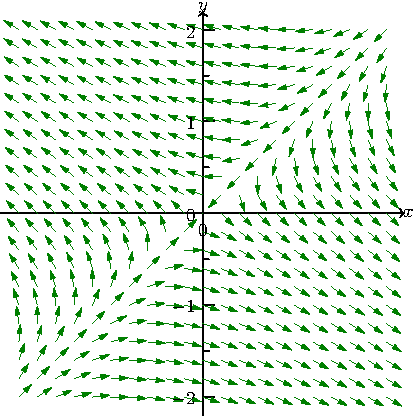
\includegraphics[width=\linewidth]{generated/asymptote/image-15.pdf}
\end{image}%
\tcblower
\end{figureptx}%
Vector fields can also be plotted easily using SageMath. The code cell below demonstrates the use of the \mono{plot\_vector\_field} command to sketch the phase portrait from \hyperref[x:example:example-sketch-phase-portrait]{Example~{\xreffont\ref{x:example:example-sketch-phase-portrait}}}.%
\begin{sageinput}
var('y1 y2') # define from system variables
VF=plot_vector_field([2*y1 - 3*y2,-2*y1 + y2],[y1,-2,2],[y2,-2,2]) # creates plot of phase portrait from system
show(VF) # shows the plot
\end{sageinput}
Note that \(\vec{y}=\vec{0}\) is \emph{always} a solution of \(\vec{y}'=A\vec{y}\). This is because \(\vec{0}'=A\vec{0} = \vec{0}\). We call \(\vec{y} = \vec{0}\) the \terminology{equilibrium solution} or \terminology{critical point} of the system \(\vec{y}'=A\vec{y}\). In the next section, we will be concerned with the behavior of trajectories of the system \(\vec{y}'=A\vec{y}\) near the equilibrium solution. One thing we will see is that the behavior is determined in large part by the eigenvalues of the matrix \(A\).%
\par
We will classify the behavior of trajectories at the critical point \(\vec{x} = \vec{0}\) into five different cases:%
\begin{tableptx}{\textbf{}}{g:table:idp105548780022048}{}%
\centering%
{\tabularfont%
\begin{tabular}{ll}\hrulethick
Classification&Behavior at \(\vec{0}\)\tabularnewline\hrulethick
Improper node&Every trajectory except two has the same limiting tangent at \(\vec{0}\)\tabularnewline[0pt]
Proper node&For every direction \(\vec{d}\) there exists trajectory with limiting tangent \(\vec{d}\)\tabularnewline[0pt]
Saddle point&Two incoming trajectories, two outgoing trajectories; all others bypass \(\vec{0}\)\tabularnewline[0pt]
Center&\(\vec{0}\) is enclosed by infinitely many closed (repeating) trajectories\tabularnewline[0pt]
Spiral point&Trajectories spiral inwards or outwards from \(\vec{0}\)\tabularnewline\hrulethick
\end{tabular}
}%
\end{tableptx}%
\(\vec{0}\) was a saddle point in \hyperref[x:example:example-sketch-phase-portrait]{Example~{\xreffont\ref{x:example:example-sketch-phase-portrait}}} since there were incoming trajectories on the line \(y_{2} = y_{1}\) and outgoing trajectories on the line \(y_{2} = -\frac{2}{3}y_{1}\).%
\begin{example}{}{x:example:example-stability-equilibrium-solution}%
Using a phase portrait, determine the type of critical point that \(\vec{y} = \vec{0}\) is for the matrix ODE \(\vec{y}'=A\vec{y}\) where%
\begin{equation*}
\vec{y} = \begin{bmatrix}y_{1}(t) \\ y_{2}(t)\end{bmatrix}\quad\text{and}\quad A = \begin{bmatrix}3 \amp  4 \\ -4 \amp  3\end{bmatrix}.
\end{equation*}
%
\par\smallskip%
\noindent\textbf{\blocktitlefont Solution}.\hypertarget{g:solution:idp105548780032160}{}\quad{}As seen in \hyperref[x:figure:figure-classify-stability-using-phase-portrait]{Figure~{\xreffont\ref{x:figure:figure-classify-stability-using-phase-portrait}}}, every (nonzero) trajectory will spiral outward from \(\vec{y} = \vec{0}\) as \(t\to\infty\), so \(\vec{0}\) is a spiral point of this system. To see why, we only need to look at the eigenvalues of \(A\), which we find to be%
\begin{equation*}
\lambda_{1} = 3+4i,\lambda_{2} = 3-4i.
\end{equation*}
This means that the general solution of \(\vec{y}' = A\vec{y}\) must look like%
\begin{align*}
\vec{y} \amp = c_{1}e^{(3+4i)t}\vec{y}_{1} + c_{2}e^{(3-4i)t}\vec{y}_{2}\\
\amp = e^{3t}\brackets{c_{1}e^{4it}\vec{y}_{1}+c_{2}e^{-4it}\vec{y}_{2}}\\
\amp = e^{3t}\brackets{(\cos4t)\vec{x}_{1}+(\sin4t)\vec{x}_{2}}\text{.}
\end{align*}
%
\par
The real part of the eigenvalues leads to the \textasciigrave{}\textasciigrave{}growth term'{}'{} of \(e^{3t}\) appearing in the solution, which causes the trajectories to diverge as \(t\to\infty\). The imaginary part of the eigenvalues leads to the \textasciigrave{}\textasciigrave{}oscillating terms'{}'{} of \(\cos4t,\sin4t\) appearing in the solution, which gives the trajectories their spiral motion.%
\end{example}
\begin{figureptx}{The phase portrait for \hyperref[x:example:example-stability-equilibrium-solution]{Example~{\xreffont\ref{x:example:example-stability-equilibrium-solution}}}.}{x:figure:figure-classify-stability-using-phase-portrait}{}%
\begin{image}{0.25}{0.5}{0.25}%
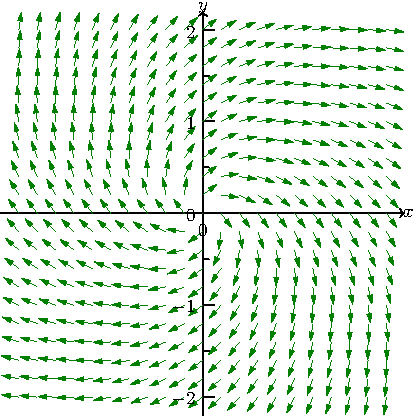
\includegraphics[width=\linewidth]{generated/asymptote/image-16.pdf}
\end{image}%
\tcblower
\end{figureptx}%
In general, the eigenvalues of the matrix \(A\) in the system \(\vec{y}' = A\vec{y}\) will determine the type of critical point that \(\vec{0}\) is for the system \(\vec{y}'=A\vec{y}\).%
\begin{example}{}{g:example:idp105548780041120}%
What kind of critical point is \(\vec{y} = \vec{0}\) for the system%
\begin{align*}
y'_{1} \amp = -4y_{2}\\
y'_{2}  \amp =  4y_{1}
\end{align*}
where \(y_{i} = y_{i}(t)\)?%
\par\smallskip%
\noindent\textbf{\blocktitlefont Solution}.\hypertarget{g:solution:idp105548780043168}{}\quad{}We could sketch the phase portrait for this system, but we can also determine the behavior of the trajectories \(\vec{y} = \begin{bmatrix} y_{1} \\ y_{2} \end{bmatrix} \) if we can find a relationship between \(y_{1}\) and \(y_{2}\). To do so, we ``cross-multiply'' the system to get%
\begin{equation*}
4y_{1}y'_{1} = -4y_{2}y'_{2} \quad\text{or}\quad 4y_{1}\dd{y_{1}} = -4y_{2}\dd{y_{2}}.
\end{equation*}
So we can integrate this to get%
\begin{equation*}
2y_{1}^{2} = -2y_{2}^{2}+C\qq{or}y_{1}^{2}+y_{2}^{2} = C_{1}.
\end{equation*}
%
\par
This is the equation of a circle of radius \(\sqrt{C_{1}}\), and so every trajectory \(\vec{y}\) for this system will be a circle centered at \(\vec{0}\). Hence \(\vec{0}\) is a center.%
\end{example}
\end{subsectionptx}
\end{sectionptx}
%
%
\typeout{************************************************}
\typeout{Section 4.3 Criteria for Critical Points; Stability}
\typeout{************************************************}
%
\begin{sectionptx}{Criteria for Critical Points; Stability}{}{Criteria for Critical Points; Stability}{}{}{x:section:section-criteria-for-critical-points-stability}
Consider the matrix ODE \(\vec{y}' = A\vec{y}\). Let \(\lambda_{1},\lambda_{2}\) denote the eigenvalues of the \(2\times 2\) matrix \(A\). Then \(\vec{0}\) is a:%
\begin{tableptx}{\textbf{Eigenvalue conditions for stability.}}{x:table:table-eigenvalue-conditions-stability}{}%
\centering%
{\tabularfont%
\begin{tabular}{ll}\hrulethick
Name&Conditions on \(\lambda_{1},\lambda_{2}\)\tabularnewline\hrulethick
Node&Real, same sign\tabularnewline[0pt]
Saddle point&Real, opposite sign\tabularnewline[0pt]
Center&Pure imaginary\tabularnewline[0pt]
Spiral point&Complex, not pure imaginary\tabularnewline\hrulethick
\end{tabular}
}%
\end{tableptx}%
The rule of thumb is this: the real parts of the eigenvalues determine whether a trajectory moves towards or away from the origin, and the imaginary part determines if the trajectory has a periodic\slash{}oscillating nature to it.%
\par
We say that the origin is a \terminology{stable} critical point of \(\vec{y}'=A\vec{y}\) if all trajectories that start \textasciigrave{}\textasciigrave{}close'{}'{} to \(\vec{0}\) remain close at all future times. Equivalently, it's stable if each trajectory will eventually be contained within some circle centered at the origin as \(t\to\infty\). Otherwise, we say that \(\vec{0}\) is \terminology{unstable}. If it so happens that every trajectory that starts close to \(\vec{0}\) tends to \(\vec{0}\) as \(t\to\infty\), we then say that \(\vec{0}\) is a \terminology{stable and attractive} (or \terminology{asymptotically stable}) critical point. Equivalently, \(\vec{0}\) is asymptotically stable if \emph{every} trajectory goes to \(\vec{0}\) as \(t\to\infty\).%
\begin{example}{}{g:example:idp105548779996192}%
Let \(\vec{y}' = A\vec{y}\) denote a matrix ODE where \(A\) is a constant \(2\times2\) matrix. What conditions on the eigenvalues of \(A\) will give an asymptotically stable critical point at \(\vec{y}=\vec{0}\)?%
\par\smallskip%
\noindent\textbf{\blocktitlefont Solution}.\hypertarget{g:solution:idp105548779998624}{}\quad{}Let \(\vec{y} = \vec{y}(t)\) denote a nonzero solution of the matrix ODE (and therefore a trajectory). Then in order for \(\vec{0}\) to be asymptotically stable, we need \(\vec{y}\to\vec{0}\) as \(t\to\infty\). Let \(\lambda_{1},\lambda_{2}\) denote the eigenvalues of \(A\). Then \(\vec{y}\) will have the form%
\begin{equation*}
\vec{y} = c_{1}e^{\lambda_{1}t}\vec{y}_{1}+c_{2}e^{\lambda_{2}t}\vec{y}_{2}.
\end{equation*}
%
\par
This will go to \(\vec{0}\) as \(t\to\infty\) if either \(c_{1}=c_{2}=0\) or if each exponential goes to \(0\) as \(t\to\infty\). Since we assume \(\vec{y}\neq\vec{0}\), this means we need \(e^{\lambda_{i}t}\to0\) for \(i=1,2\) as \(t\to\infty\). This means that the \emph{real part} of each eigenvalue must be negative. This is because the real part of each eigenvalue determines the growth of \(e^{\lambda_{i}t}\): if \(\lambda_{i} = a+bi\), then%
\begin{equation*}
e^{\lambda_{i}t} = e^{at}[A\cos bt+B\sin bt]\text{.}
\end{equation*}
So \(\vec{0}\) is asymptotically stable if the real parts of \emph{both} eigenvalues are negative.%
\end{example}
Similarly, we can say that \(\vec{0}\) is stable as long as the real part of each eigenvalue is no greater than \(0\). \(\vec{0}\) is unstable if the real part of \textbackslash{}emph\textbraceleft{}any\textbraceright{} eigenvalue is positive.%
\begin{example}{}{g:example:idp105548780009632}%
Two tanks \(T_{1}\) and \(T_{2}\) containing \SI{200}{\gallon} each of a water-salt mixture are set up as follows:%
%
\begin{itemize}[label=\textbullet]
\item{}Tank 1: Pure water flows in at \SI{12}{\gallon\per\minute} and solution from Tank 2 flows in at \SI{4}{\gallon\per\minute}; solution also flows out of Tank 1 and into Tank 2 at \SI{16}{\gallon\per\minute}.%
\item{}Solution from Tank 1 flows in at \SI{16}{\gallon\per\minute}; solution flows out of Tank 2 and into Tank 1 at \SI{4}{\gallon\per\minute}, and solution is emptied from Tank 2 at an addition rate of \SI{12}{\gallon\per\minute}%
\end{itemize}
Will the salt eventually empty from both tanks?%
\par\smallskip%
\noindent\textbf{\blocktitlefont Solution}.\hypertarget{g:solution:idp105548780019488}{}\quad{}Let \(y_{1}(t)\) denote the amount of salt (in pounds) in Tank 1 at time \(t\) (in minutes), and let \(y_{2}(t)\) do the same for Tank 2. Then%
\begin{align*}
y'_{1}  \amp =  4\frac{y_{2}}{200} - 16\frac{y_{1}}{200}\\
y'_{2}  \amp =  16\frac{y_{1}}{200} - 16\frac{y_{2}}{200}\text{.}
\end{align*}
%
\par
This is equivalent to the matrix ODE \(\vec{y}' = A\vec{y}\) where%
\begin{equation*}
\vec{y} = \begin{bmatrix}y_{1}\\y_{2}\end{bmatrix}\quad\text{and}\quad A = \begin{bmatrix}-\frac{2}{25} \amp  \frac{1}{50} \\ \frac{2}{25} \amp  -\frac{2}{25}\end{bmatrix}.
\end{equation*}
%
\par
The eigenvalues of \(A\) are%
\begin{equation*}
\lambda_{1} = -\frac{1}{25}\quad\text{and}\quad\lambda_{2} = -\frac{3}{25}.
\end{equation*}
Since both eigenvalues have negative real part, it follows that \(\vec{0}\) is an asymptotically stable critical point of \(\vec{y}'=A\vec{y}\). Therefore \emph{every} trajectory \(\vec{y}\to\vec{0}\) as \(t\to\infty\). So no matter how much salt is initially in the tanks, the amount of salt will always go to \(0\).%
\end{example}
\end{sectionptx}
%
%
\typeout{************************************************}
\typeout{Section 4.4 Nonlinear Systems}
\typeout{************************************************}
%
\begin{sectionptx}{Nonlinear Systems}{}{Nonlinear Systems}{}{}{x:section:section-nonlinear-systems}
\begin{introduction}{}%
Now we apply phase plane methods to study \terminology{nonlinear autonomous systems}, \begin{aside}{}{g:aside:idp105548779962528}%
\emph{Autonomous} just means we can write the system without explicitly referring to the independent variable \(t\).%
\end{aside}
 which for systems involving two ODEs take the form%
\begin{align*}
y'_{1} \amp = f_{1}(y_{1},y_{2})\\
y'_{2} \amp = f_{2}(y_{1},y_{2})\text{.}
\end{align*}
where \(y_{i} = y_{i}(t)\).%
\par
We can also write such a system as a vector equation:%
\begin{equation}
\vec{y}' = \vec{f}(\vec{y})\text{.}\label{x:men:equation-nonlinear-system}
\end{equation}
although not as a matrix ODE (if \(f_{i}\) are nonlinear).%
\par
Just as in the previous sections, the \terminology{phase plane} is still the \(y_{1}y_{2}-plane\), \terminology{trajectories} are still the solutions \(\vec{y}\) of \hyperref[x:men:equation-nonlinear-system]{({\xreffont\ref{x:men:equation-nonlinear-system}})} (represented as curves in the phase plane), and the \terminology{phase portrait} of \hyperref[x:men:equation-nonlinear-system]{({\xreffont\ref{x:men:equation-nonlinear-system}})} is the set of all trajectories in the phase plane. We call a point \(P\) in the phase plane a \terminology{critical point} of \hyperref[x:men:equation-nonlinear-system]{({\xreffont\ref{x:men:equation-nonlinear-system}})} if it is a solution of the same system. Equivalently, the critical points of \hyperref[x:men:equation-nonlinear-system]{({\xreffont\ref{x:men:equation-nonlinear-system}})} are precisely those points \((y_{1},y_{2})\) for which%
\begin{equation*}
f_{1}(y_{1},y_{2}) = 0\quad\text{and}\quad f_{2}(y_{1},y_{2}) = 0.  
\end{equation*}
%
\begin{example}{}{g:example:idp105548779971616}%
Express the \emph{pendulum equation} \(\theta''+\frac{g}{l}\sin\theta=0\), where \(\theta=\theta(t)\) represents the angular displacement of a pendulum from the vertical, as a nonlinear system \(\vecm{\theta}' = \vec{f}(\vecm{\theta})\) and then find its critical points.%
\par\smallskip%
\noindent\textbf{\blocktitlefont Solution}.\hypertarget{g:solution:idp105548779973664}{}\quad{}First, we have to rewrite the pendulum ODE as a first order system. We can do this without too much trouble as follows: set%
\begin{equation*}
\theta_{1} = \theta\quad\text{and}\quad\theta_{2} = \theta_{1}' = \theta'\text{.}
\end{equation*}
Then the ODE \(\theta''+\frac{g}{l}\sin\theta = 0\) turns into the system%
\begin{align*}
\theta'_{1} \amp = \theta_{2}\\
\theta'_{2} \amp = -\frac{g}{l}\sin\theta_{1}\text{,}
\end{align*}
which we can also write as \(\boldsymbol{\theta}' = \vec{f}(\boldsymbol{\theta})\) using%
\begin{equation*}
\vecm{\theta} = \begin{bmatrix}\theta_{1} \\ \theta_{2}\end{bmatrix}\quad\text{and}\quad \vec{f}(\vecm{\theta}) = \begin{bmatrix}\theta_{2} \\ -\frac{g}{l}\sin\theta_{2}\end{bmatrix}.
\end{equation*}
%
\par
Now we need to find the critical points \(\vecm{\theta}\) in the \(\theta_{1}\theta_{2}\)-plane that make \(\vec{f}(\vecm{\theta}) = \vec{0}\). So we need \(\theta_{2} = 0\) and \(\theta_{1} = \pm k\pi\) for \(k=0,\pm1,\pm2,\dots\). So the critical points of this system are all points of the form \((\pm k\pi,0)\).%
\end{example}
\end{introduction}%
%
%
\typeout{************************************************}
\typeout{Subsection  Classification of Critical Points and Linearization}
\typeout{************************************************}
%
\begin{subsectionptx}{Classification of Critical Points and Linearization}{}{Classification of Critical Points and Linearization}{}{}{x:subsection:subsection-classification-of-critical-points-and-linearization}
Critical points of systems are important because they can represent long-term behavior of a system. For example, if we have a first-order system representing the population of two species, and it turns out the the origin is asymptotically stable, then this suggests that both species could be driven to extinction. So we want to classify critical points for nonlinear systems in addition to what we have already for linear systems; unfortunately, nonlinear systems are often difficult, if not outright impossible, to solve exactly.%
\par
Thankfully, in many cases we can approximate a nonlinear system \(\vec{y}' = \vec{f}(\vec{y})\) with critical points \(P_{i}\) by a suitably chosen linear system \(\vec{y}' = A\vec{y}\) at each critical point \(P_{i}\); we call such a system the \terminology{linearization} at \(P_{i}\).%
\begin{definition}{The Jacobian of a Nonlinear System.}{x:definition:definition-the-jacobian-of-a-nonlinear-system}%
Let%
\begin{equation*}
\vec{y} = \begin{bmatrix}y_{1} \\ y_{2}\end{bmatrix}\quad\text{and}\quad\vec{f}(\vec{y}) = \begin{bmatrix}f_{1}(y_{1},y_{2}) \\ f_{2}(y_{1},y_{2})\end{bmatrix}.
\end{equation*}
The \terminology{Jacobian} of \(\vec{f}\) is the matrix \(J(y_{1},y_{2})\) given by%
\begin{equation*}
J(y_{1},y_{2}) = \begin{bmatrix}\pdv{f_{1}}{y_{1}} \amp  \pdv{f_{1}}{y_{2}} \\ \pdv{f_{2}}{y_{1}} \amp  \pdv{f_{2}}{y_{2}}\end{bmatrix}.
\end{equation*}
%
\end{definition}
The linearization of \(\vec{y}' = \vec{f}(\vec{y})\) at the point \(P = (p_{1},p_{2})\) is the linear system \(\vec{y}' = A\vec{y}\), where%
\begin{equation*}
A = J(p_{1},p_{2}).
\end{equation*}
%
\begin{example}{}{g:example:idp105548779922336}%
Find the linearization of the pendulum system \(\vecm{\theta}' = \vec{f}(\vecm{\theta})\) at the critical point \((0,0)\).%
\par\smallskip%
\noindent\textbf{\blocktitlefont Solution}.\hypertarget{g:solution:idp105548779923616}{}\quad{}For this system, we have \(f_{1}(\theta_{1},\theta_{2}) = \theta_{2}\) and \(f_{2}(\theta_{1},\theta_{2}) = -\frac{g}{l}\sin\theta_{1}\). The Jacobian is then given by%
\begin{equation*}
J(\theta_{1},\theta_{2}) = \begin{bmatrix}0 \amp  1 \\ -\frac{g}{l}\cos\theta_{1} \amp  0\end{bmatrix}.
\end{equation*}
So to get the linearization we need to set%
\begin{equation*}
A = J(0,0) = \begin{bmatrix}0 \amp  1 \\ -\frac{g}{l} \amp  0\end{bmatrix}.
\end{equation*}
%
\end{example}
The linearization of a nonlinear system isn't just useful for approximating the nonlinear system. It's also incredibly useful for classifying the critical points of a nonlinear system; for the most part, the eigenvalues of the matrix \(A\) from the linearization also classify the critical points of the system \(\vec{y}' = \vec{f}(\vec{y})\).%
\begin{example}{}{g:example:idp105548779926688}%
Find and classify the critical points of the nonlinear system%
\begin{align*}
\dv{x}{t} \amp = x - y - x^{2} + xy \\
\dv{y}{t} \amp = -x^{2} - y \text{.}
\end{align*}
%
\begin{aside}{}{g:aside:idp105548779927968}%
This example taken from \href{https://www.math.uci.edu/\~ndonalds/math3d/nonlinear.pdf}{here.}\footnotemark{}%
\end{aside}
\par\smallskip%
\noindent\textbf{\blocktitlefont Solution}.\hypertarget{g:solution:idp105548779929120}{}\quad{}The critical points occur at \(x' = y' = 0\). If we set \(x' = y'\) and solve the resulting equation, we get \(x = 0\) or \(y = -1\). If \(x = 0\), then \(x' = -y\), and for this to be \(0\) we must have \(y = 0\). We can verify that \(x = y = 0\) makes \(y' = 0\) as well, so the origin is a critical point. Similarly, \(y = -1\) forces \(x = \pm1\), and we can verify that \(x' = y' = 0\) at \((-1,-1)\) and \((1,-1)\). So we have three critical points to check.%
\par
To determine the behavior of solutions at these critical points, we'll find the Jacobian at each point. First, we have%
\begin{equation*}
J(x,y) = \begin{bmatrix} 1 - 2x + y \amp x - 1 \\ -2x \amp -1\end{bmatrix}\text{.}
\end{equation*}
At \((0,0)\), we get%
\begin{equation*}
J(0,0) = \begin{bmatrix} 1 \amp -1 \\ 0 \amp -1\end{bmatrix}\text{.}
\end{equation*}
The eigenvalues are \(1\) and \(-1\), meaning that this critical point is a saddle point. At \((-1,-1)\) we get%
\begin{equation*}
J(-1,-1) = \begin{bmatrix}2 \amp -2 \\ 2 \amp -1\end{bmatrix}
\end{equation*}
which has eigenvalues \(\lambda = \frac{1}{2}\pm\frac{1}{2}\sqrt{7}i\). Hence \((-1,-1)\) should be a spiral point. Finally, at \((1,-1)\) we get%
\begin{equation*}
J(1,-1) = \begin{bmatrix} -2 \amp 0 \\ -2 \amp -1\end{bmatrix}\text{,}
\end{equation*}
which has eigenvalues \(-2,-1\). Hence \((1,-1)\) is an asymptotically stable node.%
\end{example}
\footnotetext[1]{\nolinkurl{https://www.math.uci.edu/\~ndonalds/math3d/nonlinear.pdf}\label{g:fn:idp105548779928736}}%
We can also use nonlinear systems to get more accurate population models.%
\begin{example}{}{g:example:idp105548779940768}%
Predator-prey populations can be modeled using the Lotka-Volterra model. Let \(y_{1}(t)\) denote the population of a prey species at time \(t\) and let \(y_{2}(t)\) denote the population of a predator species at time \(t\). Then the Lotka-Volterra model says that%
\begin{align*}
y'_{1} \amp = ay_{1}-by_{1}y_{2}\\
y'_{2} \amp = ky_{1}y_{2} - ly_{2}\text{,}
\end{align*}
where \(a,b,k,l>0\). Find and classify the critical points of this system.%
\par\smallskip%
\noindent\textbf{\blocktitlefont Solution}.\hypertarget{g:solution:idp105548779943968}{}\quad{}The critical points are the points \((y_{1},y_{2})\) that satisfy the equations%
\begin{equation*}
ay_{1}-by_{1}y_{2} = 0\quad\text{and}\quad ky_{1}y_{2} - ly_{2} = 0.
\end{equation*}
Equivalently, we need%
\begin{equation*}
y_{1}(a-by_{2}) = 0\quad\text{and}\quad y_{2}(ky_{1}-l) = 0.
\end{equation*}
This has solutions \(y_{1} = y_{2} = 0\) and \(y_{1} = \frac{l}{k},y_{2} = \frac{a}{b}\). So the critical points are \((0,0)\) and \((\frac{l}{k},\frac{a}{b})\).%
\par
To classify these critical points we need to linearize the system, so we'll compute the Jacobian of%
\begin{equation*}
\vec{f}(\vec{y}) = \begin{bmatrix}ay_{1}-by_{1}y_{2} \\ ky_{1}y_{2} - ly_{2}\end{bmatrix}
\end{equation*}
to get%
\begin{equation*}
J(y_{1},y_{2}) = \begin{bmatrix}a-by_{2} \amp  -by_{1} \\ ky_{2} \amp  ky_{1} - l\end{bmatrix}.
\end{equation*}
%
\par
At \((0,0)\), we get%
\begin{equation*}
A = \begin{bmatrix}a \amp  0 \\ 0 \amp  -l\end{bmatrix}\text{,}
\end{equation*}
which has eigenvalues \(\lambda=a,-l\). So the origin is an saddle point of the original system. In particular, there exist trajectories heading into the origin, so it's possible for both species to go extinct in this case.%
\par
Now we'll classify the second critical point \((\frac{l}{k},\frac{a}{b})\). The Jacobian at this point gives us the matrix%
\begin{equation*}
A = J(\frac{l}{k},\frac{a}{b}) = \begin{bmatrix}0 \amp  -\frac{bl}{k} \\ \frac{ak}{b} \amp  0\end{bmatrix}\text{.}
\end{equation*}
This matrix has characteristic equation \(\lambda^{2} + al = 0\), and so has eigenvalues \(\lambda=\pm i\sqrt{al}\). Since the eigenvalues are pure imaginary, this suggests that \((\frac{l}{k},\frac{a}{b})\) is a center, which is indeed the case. In particular, trajectories near this critical point \emph{must be periodic}.%
\end{example}
\end{subsectionptx}
\end{sectionptx}
\end{chapterptx}
  %
%
\typeout{************************************************}
\typeout{Chapter 5 Series Solutions of ODEs}
\typeout{************************************************}
%
\begin{chapterptx}{Series Solutions of ODEs}{}{Series Solutions of ODEs}{}{}{x:chapter:series-solutions}
%
%
\typeout{************************************************}
\typeout{Section 5.1 Power Series Method}
\typeout{************************************************}
%
\begin{sectionptx}{Power Series Method}{}{Power Series Method}{}{}{x:section:section-power-series-method}
In calculus, it's important to know how to differentiate and integrate functions. For some functions (say, \(x-1,x^{2},3-x^{5}\)) it can be very straightforward, but for others (such as \(e^{-x^{2}}\)) it can be impossible. \begin{aside}{}{g:aside:idp105548781201440}%
At least, it can be impossible to integrate certain functions in terms of more \textasciigrave{}\textasciigrave{}everyday'{}'{} functions that we're used to.%
\end{aside}
%
\par
So we'd like to see if there's a way to write complicated functions \(f(x)\) in terms of simpler functions \(1,x,x^{2},\dots\). To see how, let \(f(x)\) be a function. Our goal is to write it in the form%
\begin{equation}
f(x) = c_{0}+c_{1}x+c_{2}x^{2}+c_{3}x^{3}+\dots = \sum_{k=0}^{\infty}c_{k}x^{k}\label{x:men:equation-power-series-at-zero}
\end{equation}
where the \(c_{k}\) are constants.%
\begin{definition}{Power Series.}{x:definition:definition-power-series}%
A \terminology{power series} is a series (that is, an infinite sum) of the form \(\sum_{k=0}^{\infty}c_{k}x^{k}\). Since a power series is in general an infinite sum, it may not make sense for all values of \(x\). The power series is said to \terminology{converge} on some interval \(I\) if the sum exists for each \(x\) in \(I\).%
\end{definition}
A power series doesn't have to start at \(k=0\), but \emph{it may not contain any negative powers of \(x\)}.%
\par
The question now is, how do we find the right values of the coefficients \(c_{k}\) to make \hyperref[x:men:equation-power-series-at-zero]{({\xreffont\ref{x:men:equation-power-series-at-zero}})} true? If we look at the equation, we can solve for \(c_{0}\) very easily: just set \(x=0\) to make all other terms disappear:%
\begin{equation*}
f(0) = c_{0} + c_{1}\cdot0+\dots = c_{0}.
\end{equation*}
To solve for \(c_{1}\) by plugging in \(x=0\), we need to get rid of the power of \(x\) attached to it. We can do this by taking the derivative of \(f(x)\):%
\begin{align*}
f'(x) \amp= c_{1} + 2c_{2}x + 3c_{3}x^{2} + \dots\\
f'(0) \amp= c_{1}\text{.}
\end{align*}
The same trick works for \(c_{2}\):%
\begin{align*}
f''(x) \amp= 2\cdot1c_{2} + 3\cdot2c_{3}x+\dots\\
f''(0) \amp= 2\cdot1c_{2}
\end{align*}
so \(c_{2} = \frac{f''(0)}{2\cdot1}\). Let's try this one more time to get \(c_{3}\):%
\begin{align*}
f^{(3)}(x) \amp= 3\cdot2\cdot1c_{3} + \dots\\
f^{(3)}(0) \amp= 3\cdot2\cdot1c_{3}
\end{align*}
and so \(c_{3} = \frac{f^{(3)}(0)}{3\cdot2\cdot1}\).%
\par
In general, to get the coefficient \(c_{k}\) of \(x^{k}\) in the power series of \(f(x)\), we have the following equation:%
%
\begin{equation}
c_{k} = \frac{f^{(k)}(0)}{k\cdot(k-1)\cdot\dots\cdot2\cdot1} = \frac{f^{(k)}(0)}{k!}.\label{x:men:equation-power-series-coefficients-at-zero}
\end{equation}
\begin{example}{}{x:example:example-series-exponential}%
Find a power series for \(e^{x}\).%
\par\smallskip%
\noindent\textbf{\blocktitlefont Solution}.\hypertarget{g:solution:idp105548781219488}{}\quad{}Any power series for \(f(x) = e^{x}\) looks like \(\sum_{k=0}^{\infty}c_{k}x^{k}\), where%
\begin{equation*}
c_{k} = \frac{f^{(k)}(0)}{k!}.
\end{equation*}
Since \(e^{x}\) is its own derivative, \(f^{(k)}(x) = e^{x}\) for all choices of \(k\). So%
\begin{equation*}
c_{k} = \frac{e^{0}}{k!} = \frac{1}{k!}
\end{equation*}
and the power series for \(e^{x}\) is%
\begin{equation*}
1+x+\frac{x^{2}}{2}+\frac{x^{3}}{6} + \dots = \sum_{k=0}^{\infty}\frac{x^{k}}{k!}.
\end{equation*}
It turns out the \(f(x) = e^{x}\) equals its power series for \emph{all} values of \(x\).%
\end{example}
The above power series was written in terms of powers of \(x\), but this doesn't have to be the case. We can also write power series in terms of powers of \(x-a\), where \(a\) is some constant. A power series of the form%
\begin{equation*}
\sum_{k=0}^{\infty}c_{k}(x-a)^{k}
\end{equation*}
is said to be \terminology{centered at \(a\)}. For such a series, the formula for the \(c_{k}\) is given by%
\begin{equation*}
c_{k} = \frac{f^{(k)}(a)}{k!}.
\end{equation*}
%
\begin{example}{}{x:example:example-series-sin-pi-over-2}%
Find the power series for \(g(t) = \sin t\) centered at \(a = \frac{\pi}{2}\).%
\par\smallskip%
\noindent\textbf{\blocktitlefont Solution}.\hypertarget{g:solution:idp105548781229088}{}\quad{}A power series centered at \(a = \frac{\pi}{2}\) will look like%
\begin{equation*}
\sum_{k=0}^{\infty}c_{k}\parens{t-\frac{\pi}{2}}^{k}
\end{equation*}
where%
\begin{equation*}
c_{k} = \frac{g^{(k)}(\frac{\pi}{2})}{k!}.
\end{equation*}
To find these values, we need to compute the derivatives of \(g(t)\) and evaluate them at \(\frac{\pi}{2}\):%
\begin{align*}
g^{(0)}(t) \amp= \sin t \amp\Rightarrow g^{(0)}(\frac{\pi}{2}) = 1\\
g'(t) \amp= \cos t \amp\Rightarrow g'(\frac{\pi}{2}) = 0\\
g''(t) \amp= -\sin t \amp\Rightarrow g''(\frac{\pi}{2}) = -1\\
g^{(3)}(t) \amp= -\cos t \amp\Rightarrow g^{(3)}(\frac{\pi}{2}) = 0\text{.}
\end{align*}
So the power series centered at \(\frac{\pi}{2}\) is%
\begin{equation*}
1 - \frac{1}{2!}(t-\frac{\pi}{2})^{2} + \frac{1}{4!}(t-\frac{\pi}{2})^{4}+\dots = \sum_{k=0}^{\infty}(-1)^{k}\frac{(t-\frac{\pi}{2})^{2k}}{(2k)!}.
\end{equation*}
Just as with \(e^{x}\), \(\sin t\) is equal to its power series everywhere.%
\end{example}
More functions in terms of power series:%
\begin{align*}
\frac{1}{1-x} \amp= \sum_{n=0}^{\infty}x^{n} \amp \amp= 1 + x + x^{2} + x^{3} + \cdots\\
e^{x} \amp= \sum_{n=0}^{\infty}\frac{x^{n}}{n!} \amp \amp= 1 + x + \frac{x^{2}}{2!} + \frac{x^{3}}{3!} + \cdots\\
\sin x \amp= \sum_{n=0}^{\infty}(-1)^{n}\frac{x^{2n+1}}{(2n+1)!} \amp \amp= x - \frac{x^{3}}{3!} + \frac{x^{5}}{5!} - \cdots\\
\cos x \amp= \sum_{n=0}^{\infty}(-1)^{n}\frac{x^{2n}}{(2n)!} \amp \amp= 1 - \frac{x^{2}}{2!} + \frac{x^{4}}{4!} - \cdots
\end{align*}
Viewing a function as a power series can be extremely beneficial; if you have a power series expression for some function, it is extremely easy to do calculus with it.%
\begin{example}{}{x:example:example-series-integral}%
Find \(\displaystyle\int_{0}^{1}e^{x^{2}}\dd{x}\).%
\par\smallskip%
\noindent\textbf{\blocktitlefont Solution}.\hypertarget{g:solution:idp105548781171488}{}\quad{}We can't integrate \(e^{x^{2}}\) using elementary functions \begin{aside}{}{g:aside:idp105548781172256}%
We can use a function known as the \terminology{error function}.%
\end{aside}
 but this is straightforward to integrate using power series:%
\begin{align*}
\int_{0}^{1}e^{x^{2}}\dd{x} \amp= \int_{0}^{1}\sum_{n=0}^{\infty}\frac{x^{2n}}{n!}\dd{x}\\
\amp= \sum_{n=0}^{\infty}\int_{0}^{1}\frac{x^{2n}}{n!}\dd{x}\\
\amp= \sum_{n=0}^{\infty}\frac{1}{(2n+1)n!}\text{.}
\end{align*}
%
\end{example}
The following theorem can be used to determine when a power series converges (that is, when the series makes sense).%
\begin{theorem}{}{}{x:theorem:theorem-finding-radius-convergence}%
Given the power series \(\sum_{n=0}^{\infty}c_{n}x^{n}\), define the number \(\rho\) by the limit%
\begin{equation*}
\rho = \limit{n}{\infty}\left|\frac{c_{n}}{c_{n+1}}\right|.
\end{equation*}
Suppose the limit exists or is infinite. Then \(\rho\) is the radius of converengence of the series: if \(\rho\neq0\) then the series converges for \(|x|\lt\rho\) and diverges for \(|x|\gt\rho\). If \(\rho=0\) then the series converges only at \(x=0\).%
\end{theorem}
Our main use of power series will be in solving differential equations.%
\begin{example}{}{x:example:example-series-solve-first-order-linear}%
Solve the ODE given by%
\begin{equation*}
\dv{y}{x} = 4y.
\end{equation*}
%
\par\smallskip%
\noindent\textbf{\blocktitlefont Solution}.\hypertarget{g:solution:idp105548781179808}{}\quad{}We could easily solve this using Chapter 1 methods, but we'll use power series to practice. To start, we assume that the solution \(y\) can be written as a power series:%
\begin{equation*}
y = \sum_{n=0}^{\infty}c_{n}x^{n}.
\end{equation*}
The next step is to plug this into the ODE. Since%
\begin{align*}
\dv{y}{x} \amp= \dv{}{x}\parens{\sum_{n=0}^{\infty}c_{n}x^{n}}\\
\amp= \sum_{n=1}^{\infty}nc_{n}x^{n-1}
\end{align*}
we get the equation%
\begin{equation*}
\sum_{n=1}^{\infty}nc_{n}x^{n-1} = 4\sum_{n=0}^{\infty}c_{n}x^{n}\text{.}
\end{equation*}
%
\par
We need to find the values of the coefficients \(c_{n}\); we do this by equating coefficients on both sides of the equation. We want to write both series in terms of \(x^{n}\) so that we can do this, so we need to shift the summation on the left: we replace \(n\) with \(n+1\) inside the sum and decrease the limit of summation \(n=1\) to \(n=0\) to get%
\begin{equation*}
\sum_{n=0}^{\infty}(n+1)c_{n+1}x^{n} = \sum_{n=0}^{\infty}4c_{n}x^{n}\text{.}
\end{equation*}
Now we can equate coefficients: for \(n\geq0\), we have%
\begin{equation*}
(n+1)c_{n+1} = 4c_{n}\qq{or} c_{n+1} = \frac{4}{n+1}c_{n}.
\end{equation*}
%
\par
This is known as a \terminology{recurrence relation}. It describes the coefficients in terms of the previous ones, and can be used to determine explicitly what each \(c_{n}\) looks like. To see how, we plug several values for \(n\) into this recurrence relation to try to determine a pattern:%
\begin{align*}
c_{1} \amp= \frac{4}{2}c_{0}\\
c_{2} \amp= \frac{4}{3}c_{1} = \frac{4^{2}}{3\cdot2}c_{0}\\
c_{3} \amp= \frac{4}{4}c_{2} = \frac{4^{3}}{4\cdot3\cdot2}c_{0}
\end{align*}
and in general it appears that%
\begin{equation*}
c_{n} = \frac{4^{n}}{n!}c_{0}
\end{equation*}
for each \(n\). \begin{aside}{}{g:aside:idp105548781189280}%
We can't solve for \(c_{0}\) without specifying an initial condition of some kind.%
\end{aside}
 So the solution \(y\) is%
\begin{align*}
y \amp= \sum_{n=0}^{\infty}c_{n}x^{n}\\
\amp= \sum_{n=0}^{\infty}\frac{4^{n}}{n!}c_{0}x^{n}\\
\amp= c_{0}\sum_{n=0}^{\infty}\frac{(4x)^{n}}{n!}\\
\amp= c_{0}e^{4x}\text{.}
\end{align*}
%
\end{example}
To solve the above ODE we used the following steps:%
\begin{enumerate}
\item{}Write \(y = \sum_{n=0}^{\infty}c_{n}x^{n}\).%
\item{}Use the ODE to build a recurrence relation for the coefficients \(c_{n}\).%
\item{}Find an explicit description of the coefficients.%
\item{}Identify \(y\) as the power series of some function.%
\end{enumerate}
%
\begin{example}{}{g:example:idp105548781196064}%
Use power series to solve the ODE \(y^\prime+2xy=0\).%
\par\smallskip%
\noindent\textbf{\blocktitlefont Solution}.\hypertarget{g:solution:idp105548781196960}{}\quad{}We will solve this using the steps listed above. First, assume \(y = \sum_{k=0}^{\infty}c_{k}x^{k}\). Now plug this guess for \(y\) into the ODE to get%
\begin{equation*}
\sum_{k=1}^{\infty}kc_{k}x^{k-1} = -\sum_{k=0}^{\infty}2c_{k}x^{k+1}.
\end{equation*}
We want to equate coefficients to build a recurrence relation, so we need to rewrite these sums in terms of a single \(x^{n}\), as opposed to \(x^{k-1}\) and \(x^{k+1}\). We do this by shifting the sums, but we need to remember to shift the limits of each sum as well:%
\begin{center}%
{\tabularfont%
\begin{tabular}{lll}\hrulethick
Sum&Index&Limit\tabularnewline\hrulethick
\(\sum_{k=1}^{\infty}kc_{k}x^{k-1}\)&\(k-1\to n\) \textbackslash{}amp \(k=1\to n=0\)\tabularnewline[0pt]
\(-\sum_{k=0}^{\infty}2c_{k}x^{k+1}\)&\(k+1\to n\) \textbackslash{}amp \(k=0\to n=1\)\tabularnewline\hrulethick
\end{tabular}
}%
\end{center}%
So we get%
\begin{equation*}
\sum_{n=0}^{\infty}(n+1)c_{n+1}x^{n} = \sum_{n=1}^{\infty}(-2)c_{n-1}x^{n} = 0.
\end{equation*}
So a recurrence relation for \(c_{n}\) is%
\begin{equation*}
c_{n+1} = -\frac{2}{n+1}c_{n-1}\qq{for }.
\end{equation*}
%
\par
Since this \terminology{two-step recurrence relation} is only valid for \(n\geq1\), it places no restrictions on any constant terms of the series. We'll need to determine these separately. To do so, write out the first couple terms of the sums in the previous equation:%
\begin{equation*}
c_{1}+2c_{2}x+\dots = -2c_{0}x -2c_{1}x^{2}+\cdots
\end{equation*}
This tells us that \(c_{1} = 0\). Again, we can't get this information from the recurrence relation!%
\par
Now we try to find an explicit formula for \(c_{n}\). Because this is a two-step recurrence, we will write out the coefficients in two columns, one for odd \(n\) and one for even \(n\):%
\begin{align*}
c_{2} \amp= -\frac{2}{2}c_{0} \amp c_{3} \amp= -\frac{2}{3}c_{1} = 0\\
c_{4} \amp= -\frac{2}{4}c_{2} = \frac{1}{2}\frac{1}{1}c_{0} \amp c_{5} \amp= -\frac{2}{5}c_{3} = 0\\
c_{6} \amp= -\frac{2}{6}c_{4} = -\frac{1}{3}\frac{1}{2}\frac{1}{1}c_{0} \amp c_{7} \amp= -\frac{2}{7}c_{5} = 0\text{.}
\end{align*}
So it appears that%
\begin{equation*}
c_{2k} = \frac{(-1)^{k}}{k!}c_{0}\qq{and}c_{2k+1} = 0
\end{equation*}
for every \(k\).%
\par
Now we plug this into our power series for \(y\) to get%
\begin{align*}
y \amp= \sum_{k=0}^{\infty}c_{k}x^{k}\\
\amp= \sum_{k=0}^{\infty}c_{2k}x^{2k}\\
\amp= \sum_{k=0}^{\infty}c_{0}\frac{(-1)^{k}}{k!}x^{2k}\\
\amp= c_{0}\sum_{k=0}^{\infty}\frac{(-x^{2})^{k}}{k!}\\
\amp= c_{0}e^{-x^{2}}\text{.}
\end{align*}
%
\end{example}
Now that we have an idea of how to solve differential equations using power series, it can be useful to know when this method is actually valid, i.e., when power series solutions exist. We will be particularly concerned with solutions of second-order linear ODEs.%
\begin{theorem}{Existence of Series Solutions.}{}{x:theorem:theorem-existence-of-series-solutions}%
Consider the differential equation%
\begin{equation*}
y'' + P(x)y^\prime + Q(x)y = R(x)\text{.}
\end{equation*}
If \(P(x), Q(x)\) and \(R(x)\) are \terminology{analytic} at a point \(x_{0}\), then every solution is also analytic at \(x_{0}\).%
\end{theorem}
\begin{example}{A Legendre Equation.}{x:example:example-a-legendre-equation}%
Show that%
\begin{equation*}
(1 - x^{2})y'' - 2xy^\prime + 2y = 0
\end{equation*}
has a series solution centered at \(0\) and then find the solution up to the coefficient of \(x^{6}\).%
\par\smallskip%
\noindent\textbf{\blocktitlefont Solution}.\hypertarget{g:solution:idp105548781152800}{}\quad{}First, note that the equation can be rewritten%
\begin{equation*}
y'' - \frac{2x}{1 - x^{2}}y^\prime + \frac{2}{1 - x^{2}}y = 0\text{,}
\end{equation*}
so we are guaranteed a series solution centered at \(x = 0\). Furthermore, this solution has radius of convergence at least \(R = 1\).%
\par
To find the solution, we return to the original equation and substitute \(y = \sum_{n=0}^{\infty}c_{n}x^{n}\) to get%
\begin{equation*}
\sum_{n\geq0}n(n-1)c_{n}x^{n-2} - \sum_{n\geq0}n(n-1)c_{n}x^{n} - \sum_{n\geq0}2nc_{n}x^{n} + \sum_{n\geq0}2c_{n}x^{n} = 0
\end{equation*}
which becomes%
\begin{equation*}
\sum_{n\geq0}(n + 2)(n+1)c_{n+2}x^{n} - \sum_{n\geq0}n(n-1)c_{n}x^{n} - \sum_{n\geq0}2nc_{n}x^{n} + \sum_{n\geq0}2c_{n}x^{n} = 0\text{.}
\end{equation*}
After a little algebra, we get the recurrence relation%
\begin{equation*}
c_{n+2} = \frac{n-1}{n+1}c_{n}\quad\text{for}\quad n\geq2\text{.}
\end{equation*}
This recurrence is valid for \(n\geq0\).%
\par
Now we can use the recurrence to list the first several terms of the solution:%
\begin{equation*}
y = c_{1}x + c_{0}(1 - x^{2} - \frac{1}{3}x^{4} - \frac{1}{5}x^{6} - \cdots)
\end{equation*}
In fact,%
\begin{equation*}
y = c_{1}x - \sum_{n\geq0}\frac{1}{2n - 1}c_{0}x^{2n}\text{.}
\end{equation*}
%
\end{example}
\end{sectionptx}
%
%
\typeout{************************************************}
\typeout{Section 5.2 Legendre's Equation and Legendre Polynomials}
\typeout{************************************************}
%
\begin{sectionptx}{Legendre's Equation and Legendre Polynomials}{}{Legendre's Equation and Legendre Polynomials}{}{}{x:section:section-legendre-s-equation-and-legendre-polynomials}
\begin{introduction}{}%
An important differential equation in applications is the \terminology{Legendre equation} given by%
\begin{equation}
(1 - x^{2})y'' - 2xy^\prime + k(k + 1)y = 0\text{.}\label{x:men:equation-legendre-ode}
\end{equation}
Our first example of this equation (with \(n = 1\)) was examined in \hyperref[x:example:example-a-legendre-equation]{Example~{\xreffont\ref{x:example:example-a-legendre-equation}}}. By this example, we see that \hyperref[x:men:equation-legendre-ode]{({\xreffont\ref{x:men:equation-legendre-ode}})} has a series solution centered at \(x = 0\) with radius of convergence at least \(1\). Therefore the power series method is appropriate.%
\end{introduction}%
%
%
\typeout{************************************************}
\typeout{Subsection  Solving the Legendre Equation}
\typeout{************************************************}
%
\begin{subsectionptx}{Solving the Legendre Equation}{}{Solving the Legendre Equation}{}{}{x:subsection:subsection-solving-the-legendre-equation}
We'll proceed as we did in \hyperref[x:example:example-a-legendre-equation]{Example~{\xreffont\ref{x:example:example-a-legendre-equation}}}, altering the last sum as necessary to get%
\begin{equation*}
\sum_{n\geq0}(n+2)(n+1)c_{n+2}x^{n} - \sum_{n\geq0}n(n-1)c_{n}x^{n} - \sum_{n\geq0}2nc_{n}x^{n} + \sum_{n\geq0}k(k+1)c_{n}x^{n} = 0
\end{equation*}
which gives (after a bit of algebra, once again)%
\begin{equation*}
c_{n+2} = -\frac{(k - n)(k + n + 1)}{(n + 2)(n + 1)}c_{n}\text{.}
\end{equation*}
%
\par
This recurrence is valid for \(n \geq 0\), and allows us to write out the solution \(y\) in terms of the parameter \(k\) and the arbitrary constants \(c_{0}\) and \(c_{1}\):%
\begin{equation*}
y = c_{0}y_{1}(x) + c_{1}y_{2}(x)
\end{equation*}
where%
\begin{align}
y_{1}(x) \amp = 1 - \frac{k(k+1)}{2!}x^{2} + \frac{(k - 2)k(k+1)(k + 3)}{4!}x^{4} - \cdots\label{x:mrow:equation-legendre-soln-y1}\\
y_{2}(x) \amp = x - \frac{(k-1)(k+2)}{3!}x^{3} + \frac{(k-3)(k-1)(k+2)(k+4)}{5!}x^{5} - \cdots \text{.}\label{x:mrow:equation-legendre-soln-y2}
\end{align}
%
\par
Note that \(y_{1}\) and \(y_{2}\) form a basis of solutions (\hyperref[x:definition:definition-basis-of-solutions]{Definition~{\xreffont\ref{x:definition:definition-basis-of-solutions}}}) of the Legendre equation, which means that \(y = c_{0}y_{1} + c_{1}y_{2}\) must also be the general solution.%
\end{subsectionptx}
%
%
\typeout{************************************************}
\typeout{Subsection  Legendre Polynomials}
\typeout{************************************************}
%
\begin{subsectionptx}{Legendre Polynomials}{}{Legendre Polynomials}{}{}{x:subsection:subsection-legendre-polynomials}
Our solution of \hyperref[x:men:equation-legendre-ode]{({\xreffont\ref{x:men:equation-legendre-ode}})} simplifies greatly if \(k\) happens to be an integer. In particular, if \(k\) is a nonnegative integer then%
\begin{equation*}
a_{k+2} = a_{k+4} = \cdots = 0\text{.}
\end{equation*}
If \(k\) is even then the solution \(y_{1}\) given in \hyperref[x:mrow:equation-legendre-soln-y1]{({\xreffont\ref{x:mrow:equation-legendre-soln-y1}})} becomes a polynomial:%
\begin{equation*}
y_{1} = 1 - \frac{k(k+1)}{2!}x^{2} + \cdots + (-1)^{k/2}\frac{[k - (k-2)][k - (k-4)]\cdots[k + (k-3)][k + (k-1)]}{k!}x^{k}\text{.}
\end{equation*}
Likewise, if \(k\) is odd then \(y_{2}\) given in \hyperref[x:mrow:equation-legendre-soln-y2]{({\xreffont\ref{x:mrow:equation-legendre-soln-y2}})} becomes a polynomial instead:%
\begin{equation*}
y_{2} = x - \frac{(k-1)(k+2)}{3!}x^{3} + \cdots + (-1)^{\frac{k-1}{2}}\frac{[k - (k - 2)][k - (k - 4)]\cdots[k + (k - 3)][k + (k - 1)]}{k!}x^{k}\text{.}
\end{equation*}
%
\par
By choosing \(c_{0}\) and \(c_{1}\) judiciously, we can guarantee that the polynomials \(c_{0}y_{1}\) (if \(k\) is even) or \(c_{1}y_{2}\) (if \(k\) is odd) are precisely equal to \(1\) at \(x = 1\). Doing so gives us the \terminology{Legendre polynomials} \(P_{n}(x)\), defined more precisely in \hyperref[x:men:equation-legendre-poly]{({\xreffont\ref{x:men:equation-legendre-poly}})}:%
\begin{equation}
P_{n}(x) = \begin{cases} \sum_{j = 0}^{n/2}(-1)^{j}\frac{(2n - 2j)!}{2^{n}j!(n - j)!(n - 2j)!}x^{n - 2j} \amp \text{ if }n\text{ is even} \\
\sum_{j = 0}^{(n-1)/2}(-1)^{j}\frac{(2n - 2j)!}{2^{n}j!(n - j)!(n - 2j)!}x^{n - 2j} \amp \text{ if }n\text{ is odd} \\ \end{cases}\text{.}\label{x:men:equation-legendre-poly}
\end{equation}
%
\par
These polynomials satisfy several nice properties, but one of the most important characteristics they have is that \(\{P_{n}(x)\}\) forms an \emph{orthogonal set} of polynomials on the interval \([-1,1]\). This means that%
\begin{equation*}
\int_{-1}^{1}P_{m}(x)P_{n}(x)\,dx = 0
\end{equation*}
if \(m\neq n\). It can also be shown that%
\begin{equation*}
\int_{-1}^{1}P_{m}(x)P_{n}(x)\,dx = \frac{2}{2n+1}
\end{equation*}
if \(m = n\). This property allows us to express \emph{any} polynomial as a finite sum of Legendre polynomials in a computationally efficient manner. Furthermore, if we allow infinite series then we can use Legendre polynomials to express and continuous function on \([-1,1]\).%
\par
For actually computing Legendre polynomials, instead of using \hyperref[x:men:equation-legendre-poly]{({\xreffont\ref{x:men:equation-legendre-poly}})} we often use \emph{Rodrigues' formula}%
\begin{equation}
P_{n}(x) = \frac{1}{2^{n}n!}\dv[n]{}{x}[(x^{2} - 1)^{n}]\label{x:men:equation-rodrigues}
\end{equation}
or \emph{Bonnet's recurrence}%
\begin{equation}
(n + 1)P_{n + 1}(x) = (2n + 1)xP_{n}(x) - n P_{n-1}(x)\text{.}\label{x:men:equation-bonnet-recurrence}
\end{equation}
Either recurrence is simple to program into a CAS, as seen in the Sage cell below:%
\begin{sageinput}
def rodrigues(n):
    Cn = (1 / (2^n * factorial(n)))
    pn = (x^2 - 1)^n

    pretty_print( (Cn * diff(pn, n)).full_simplify() )

def bonnet(n):
    k = 1
    P0 = 1
    P1 = x
    while k < n:
        P0, P1 = P1, ((2*k + 1) / (k + 1)) * x * P1 - (k / (k + 1)) * P0
        k += 1

    pretty_print( P1.full_simplify() )

n = 9
rodrigues(n)
bonnet(n)
\end{sageinput}
\end{subsectionptx}
\end{sectionptx}
%
%
\typeout{************************************************}
\typeout{Section 5.3 Frobenius Method}
\typeout{************************************************}
%
\begin{sectionptx}{Frobenius Method}{}{Frobenius Method}{}{}{x:section:section-frobenius-method}
\begin{aside}{}{g:aside:idp105548781124000}%
This section corresponds to Section 5.3 of the text.%
\end{aside}
%
%
\typeout{************************************************}
\typeout{Subsection  Regular Points and Singular Points}
\typeout{************************************************}
%
\begin{subsectionptx}{Regular Points and Singular Points}{}{Regular Points and Singular Points}{}{}{x:subsection:subsection-regular-points-and-singular-points}
Recall that a homogeneous, linear second order ODE has the form%
\begin{equation*}
A(x)y''+B(x)y^\prime+C(x)y = 0.
\end{equation*}
We can rewrite this in the form%
\begin{equation*}
y''+P(x)y^\prime+Q(x)y = 0.
\end{equation*}
As we saw at the end of \hyperref[x:section:section-power-series-method]{Section~{\xreffont\ref{x:section:section-power-series-method}}}, the usefulness of the power series method depends on the behavior of \(P(x)\) and \(Q(x)\) at the point we're centering our series solution at.%
\begin{definition}{Regular Points and Singular Points.}{x:definition:definition-regular-points-and-singular-points}%
\index{regular and singular points}%
A point \(x=a\) is called a \terminology{regular point} if \(P(x)\) and \(Q(x)\) both have power series expansions at \(x=a\). If \(x=a\) is not a regular point we call it a \terminology{singular point}.%
\end{definition}
Regular points of an ODE are nice because of the following theorem:%
\begin{theorem}{Existence of Series Solution.}{}{x:theorem:theorem-existence-of-series-solution}%
\index{Existence of Series Solutions}%
Suppose that \(a\) is a regular point of the differential equation \(y''+P(x)y^\prime+Q(x)y=0\). Then the ODE has two linearly independent solutions of the form%
\begin{equation*}
y(x) = \sum_{n=0}^{\infty}c_{n}(x-a)^{n}.
\end{equation*}
The radius of convergence is at least as large as the distance from \(a\) to the nearest singular point of the ODE.%
\end{theorem}
In other words, \emph{the power series method works at regular points.}%
\begin{example}{}{g:example:idp105548781331360}%
Find the general solution, as a power series in powers of \(x\), for the ODE \((x^{2}+2)y''+4xy^\prime+2y=0\).%
\par\smallskip%
\noindent\textbf{\blocktitlefont Solution}.\hypertarget{g:solution:idp105548781332640}{}\quad{}The first thing we will do is make sure that the ODE actually has a power series solution at \(x=0\). To do this, we need to show that \(x=0\) is a regular point of the ODE. So we need to find \(P(x)\) and \(Q(x)\) and check that they (or their power series) make sense at \(x=0\). If we divide through the ODE by \(x^{2}+2\) we obtain%
\begin{equation*}
y''+\frac{4x}{x^{2}+2}y^\prime+\frac{2}{x^{2}+2}y = 0
\end{equation*}
so%
\begin{align*}
P(x) \amp= \frac{4x}{x^{2}+2}\\
Q(x) \amp= \frac{2}{x^{2}+2}\text{.}
\end{align*}
Since both of these exist at \(x=0\), it follows that \(x=0\) is a regular point of the ODE. Therefore the ODE has a power series solution at \(x=0\) (that is, in powers of \(x\)). Since \(P(x)\) and \(Q(x)\) both have singular points at \(x=\pm i\), it follows that the radius of convergence of the power series solution is at least \(|i - 0| = 1\).%
\begin{aside}{}{g:aside:idp105548781339552}%
Here, we're using the formula \(|a+bi| = sqrt{a^2 + b^2}.\)%
\end{aside}
We return to the original form of the ODE to solve it; if we didn't do so, we would need to expand \(P(x)\) and \(Q(x)\) using their own power series, and this would \emph{greatly} complicate the algebra. Just as we did in Section 5.1, we assume the ODE has a series solution of the form \(y = \sum_{n=0}^{\infty}c_{n}x^{n}\), or just \(y=\sum_{n\geq0}c_{n}x^{n}\) for short. Now we plug this into the ODE to get%
\begin{equation*}
(x^{2}+2)\sum_{n\geq0}^{}n(n-1)c_{n}x^{n-2}+4x\sum_{n\geq0}^{}nc_{n}x^{n-1}+2\sum_{n\geq0}^{}c_{n}x^{n} = 0
\end{equation*}
which simplifies to%
\begin{equation*}
\sum_{n\geq0}^{}n(n-1)c_{n}x^{n}+\sum_{n\geq2}^{}2n(n-1)c_{n}x^{n-2}+\sum_{n\geq0}^{}4nc_{n}x^{n}+\sum_{n\geq0}^{}2c_{n}x^{n} = 0
\end{equation*}
or just%
\begin{equation*}
\sum_{n\geq0}^{}n(n-1)c_{n}x^{n}+\sum_{n\geq0}^{}2(n+2)(n+1)c_{n+2}x^{n}+\sum_{n\geq0}^{}4nc_{n}x^{n}+\sum_{n\geq0}^{}2c_{n}x^{n} = 0
\end{equation*}
%
\par
Now we can collect like terms, and combine everything on the left hand side into one sum:%
\begin{equation*}
\sum_{n\geq0}^{}\left[n(n-1)c_{n}+2(n+2)(n+1)c_{n+2}+4nc_{n}+2c_{n}\right]x^{n} = 0.
\end{equation*}
For this sum to be \(0\) each of the coefficients must be \(0\), so we must have%
\begin{equation*}
n(n-1)c_{n}+2(n+2)(n+1)c_{n+2}+4nc_{n}+2c_{n} = 0.
\end{equation*}
We can solve this for \(c_{n+2}\) to get a recurrence relation for these coefficients:%
\begin{equation*}
2(n+2)(n+1)c_{n+2} = -c_{n}[n(n-1)+4n+2] \qq{for }
\end{equation*}
so%
\begin{equation*}
c_{n+2} = -\frac{1}{2}c_{n}\qq{for }.
\end{equation*}
%
\par
We need to find a pattern for the coefficients. Since this is a two-step relation, we'll set up two columns: one column for even \(n\) and one column for odd \(n\):%
\begin{align*}
c_{2} \amp= -\frac{1}{2}c_{0} \amp c_{3} \amp= -\frac{1}{2}c_{1}\\
c_{4} \amp= -\frac{1}{2}c_{2} = \frac{1}{2^{2}}c_{0} \amp c_{5} \amp= -\frac{1}{2}c_{3} = \frac{1}{2^{2}}c_{1}\text{.}
\end{align*}
So it appears that%
\begin{equation*}
c_{2n} = (-1)^{n}\frac{1}{2^{n}}c_{0}\qq{and}c_{2n+1} = (-1)^{n}\frac{1}{2^{n}}c_{1}\text{.}
\end{equation*}
%
\par
Therefore the general solution of the ODE is%
\begin{align*}
y \amp= \sum_{n\geq0}^{}c_{n}x^{n}\\
\amp= \sum_{n\geq0}c_{2n}x^{2n} + \sum_{n\geq0}c_{2n+1}x^{2n+1}\\
\amp= c_{0}\sum_{n\geq0}^{}(-1)^{n}\frac{x^{2n}}{2^{n}}+c_{1}\sum_{n\geq0}^{}(-1)^{n}\frac{x^{2n+1}}{2^{n}}\\
\amp= c_{0}\sum_{n\geq0}^{}\left(-\frac{x^{2}}{2}\right)^{n}+c_{1}x\sum_{n\geq0}^{}\left(-\frac{x^{2}}{2}\right)^{n}\\
\amp= \frac{c_{0}}{1+\frac{x^{2}}{2}} + \frac{c_{1}x}{1+\frac{x^{2}}{2}}
\end{align*}
%
\end{example}
\begin{sageinput}
# code cell demonstrating series calculations in Sage
# guess y = sum(c_k * x^k) for solution
vars = var('c0 c1 c2 c3 c4 c5')
y = sum([vars[k]*x^k for k in srange(0, 6)])

# plug guess into ODE and simplify
deqn = (x^2 + 2)*y.diff(x, 2) + 4*x*y.diff(x) + 2*y
deqn.collect(x)
\end{sageinput}
\end{subsectionptx}
%
%
\typeout{************************************************}
\typeout{Subsection  Solutions at Singular Points and Indicial Equations}
\typeout{************************************************}
%
\begin{subsectionptx}{Solutions at Singular Points and Indicial Equations}{}{Solutions at Singular Points and Indicial Equations}{}{}{x:subsection:subsection-solutions-at-singular-points-and-indicial-equations}
We've seen several examples showing the effectiveness of the power series method at regular points, but the situation becomes more complicated at singular points. At these points, we may not be guaranteed a power series solution.%
\begin{example}{}{g:example:idp105548781354016}%
Attempt to solve the ODE \(x^{2}y''+x^{2}y^\prime+y=0\).%
\par\smallskip%
\noindent\textbf{\blocktitlefont Solution}.\hypertarget{g:solution:idp105548781354912}{}\quad{}We start, just as we did before, by assuming the solution is a power series: \(y=\sum_{n\geq0}^{}c_{n}x^{n}\). If we plug this into the ODE and simplify somewhat, we get the equation%
\begin{equation*}
c_{0}+\sum_{n\geq2}^{}\left[n(n-1)c_{n}+(n-1)c_{n-1}+c_{n}\right]x^{n} = 0.
\end{equation*}
So it follows that%
\begin{align*}
c_{0} \amp= 0\\
c_{n} \amp= -\frac{n-1}{n(n-1)+1}c_{n-1}
\end{align*}
so the recurrence relation shows that \(c_{1} = 0, c_{2} = 0,\ldots\) so the solution would have to be \(y=0\). This is certainly a solution, but it can't be the general solution. What this tells us is that the general solution of this ODE \emph{cannot} be written as a power series.%
\end{example}
The reason we couldn't find a solution of the form \(y=\sum_{n\geq0}^{}c_{n}x^{n}\) was because \(x=0\) is a singular point of the ODE. If we divide through by \(x^{2}\) we get%
\begin{equation*}
y''+\frac{1}{x}y^\prime+\frac{1}{x^{2}}y = 0
\end{equation*}
and it's obvious that the coefficients have a divide by \(0\) problem at \(x=0\).%
\par
Our goal is to find a way of dealing with situations where \(x=0\) is a singular point of the ODE%
\begin{equation*}
x^{2}y''+xp(x)y^\prime+q(x)y=0.
\end{equation*}
We know, in general, that we won't be able to find a power series solution \(\sum_{n\geq0}^{}c_{n}x^{n}\); intuitively, a power series solution is too \textasciigrave{}\textasciigrave{}nice'{}'{} to be a solution of this ODE if \(x=0\) is a singular point. To fix this, we change our guess for \(y\) to \(y=x^{r}\sum_{n\geq0}^{}c_{n}x^{n}\) or, equivalently,%
\begin{equation*}
y = \sum_{n\geq0}^{}c_{n}x^{n+r}.
\end{equation*}
Here, \(r\) can be any number (real or complex!), so in general \(y\) \emph{will not be a power series}. \begin{aside}{}{g:aside:idp105548781298848}%
Recall that a power series, by definition, has only nonnegative whole number powers of \(x\).%
\end{aside}
 We lose a little bit by no longer assuming that \(y\) is a power series, but this expression may be flexible enough to lead to a solution of the ODE if \(x=0\) is a singular point.%
\par
Our goal now is to find the value of \(r\) based on the ODE and the coefficient functions \(p(x)\) and \(q(x)\). To do so, we will plug \(y=\sum_{n\geq0}^{}c_{n}x^{n+r}\) into the ODE%
\begin{equation*}
x^{2}y''+xp(x)y^\prime+q(x)y = 0
\end{equation*}
and attempt to get some conditions on \(r\). First, note that%
\begin{align*}
y^\prime \amp= \sum_{n\geq0}^{}(n+r)c_{n}x^{n+r-1}\\
y'' \amp= \sum_{n\geq0}^{}(n+r)(n+r-1)c_{n}x^{n+r-2}
\end{align*}
so when we plug these into the ODE we get%
\begin{equation*}
\sum_{n\geq0}^{}(n+r)(n+r-1)c_{n}x^{n+r}+\sum_{n\geq0}^{}p(x)(n+r)c_{n}x^{n+r}+\sum_{n\geq0}^{}q(x)c_{n}x^{n+r} = 0.
\end{equation*}
Now combine everything into one sum to get%
\begin{equation*}
\sum_{n\geq0}^{}\left[(n+r)(n+r-1)+p(x)(n+r)+q(x)\right]c_{n}x^{n+r} = 0.
\end{equation*}
So for this equation to be true, we need to have%
\begin{equation*}
\left[(n+r)(n+r-1)+p(x)(n+r)+q(x)\right]c_{n} = 0
\end{equation*}
for every \(n\) and every \(x\). Since we are trying to find \(r\), we'll pick values for \(n\) and \(x\). In particular, if we assume that \(p(x)\) and \(q(x)\) exist at \(x=0\) we can pick \(n=x=0\) to get%
\begin{equation*}
r(r-1)+p(0)r+q(0) = 0
\end{equation*}
(we can assume that \(c_{0}\neq0\)). This equation tells us how to find \(r\).%
\begin{definition}{Indicial Equation.}{x:definition:definition-indicial-equation}%
\index{indicial equation}%
Suppose that \(x=0\) is a singular point of the ODE%
\begin{equation*}
x^{2}y''+xp(x)y^\prime+q(x)y=0
\end{equation*}
but that \(p(x)\) and \(q(x)\) have well-defined power series at \(x=0\) (i.e. \(p(0)\) and \(q(0)\) make sense). The \terminology{indicial equation} is given by%
\begin{equation*}
r(r-1)+p(0)r+q(0) = 0.
\end{equation*}
%
\end{definition}
What we've shown is that if \(y=x^{r}\sum_{n\geq0}^{}c_{n}x^{n}\) is a solution of the ODE%
\begin{equation*}
x^{2}y''+xp(x)y^\prime+q(x)y=0
\end{equation*}
then \(r\) must be a root of the indicial equation. In fact, we can say more.%
\begin{theorem}{Method of Frobenius.}{}{x:theorem:theorem-method-of-frobenius}%
\index{Method of Frobenius}%
Consider the ODE%
\begin{equation*}
x^{2}y''+xp(x)y^\prime+q(x)y=0.
\end{equation*}
Let \(r_{1}\geq r_{2}\) be (real) roots of the indicial equation \(r(r-1)+p(0)r+q(0)=0\).%
\begin{enumerate}
\item{}There is a solution of the ODE of the form \(y_{1}(x) = x^{r_{1}}\sum_{n\geq0}^{}c_{n}x^{n}\).%
\item{}If \(r_{1}-r_{2}\) is \emph{not} equal to an integer, then there exists a second linearly independent solution of the form \(y_{2}(x) = x^{r_{2}}\sum_{n\geq0}^{}d_{n}x^{n}\).%
\item{}If \(r_{1} = r_{2}\), there exists a second linearly independent solution of the form \(y_{2}(x) = y_{1}(x)\ln x + x^{r_{1}}(C_{0} + C_{1}x + \cdots )\).%
\item{}If \(r_{1} - r_{2}\) is a nonzero integer, there exists a second linearly independent solution of the form \(y_{2}(x) = ky_{1}(x)\ln x + x^{r_{2}}(C_{0} + C_{1}x + \cdots )\).%
\end{enumerate}
%
\end{theorem}
\begin{example}{Using the Method of Frobenius.}{x:example:example-using-method-of-frobenius}%
Find a series solution centered at \(0\) of the ODE%
\begin{equation*}
x^{2}y''+xy^\prime+(x^{2}-\frac{1}{4})y=0.
\end{equation*}
%
\par\smallskip%
\noindent\textbf{\blocktitlefont Solution}.\hypertarget{g:solution:idp105548781325472}{}\quad{}If we divide through the ODE by \(x^{2}\) we get a divide-by-zero problem at \(x=0\), so \(x=0\) is a singular point. However, for this ODE we have%
\begin{align*}
p(x) \amp= 1\\
q(x) \amp= x^{2}-\frac{1}{4}
\end{align*}
so \(p(x)\) and \(q(x)\) both have power series representations centered at \(0\) (namely, themselves!). This means we can use the method of Frobenius to find a solution of the form \(y = x^r\sum_{n=0}^{\infty}c_n x^n\).%
\par
The first step is to set up and solve the indicial equation, which in this case is given by%
\begin{equation*}
r(r-1)+r-\frac{1}{4} = 0.
\end{equation*}
We solve this algebraically for \(r\) to get the roots \(r_{1}=\frac{1}{2}\) and \(r_{2}=-\frac{1}{2}\). Since \(r_{1}-r_{2} = 1\) is an integer, we are guaranteed a solution based on \(r_{1} = \frac{1}{2}\) and a second solution based on \(r_{2} = -\frac{1}{2}\) and the logarithm. So we make the guess%
\begin{equation*}
y = x^{\frac{1}{2}}\sum_{n\geq0}^{}c_{n}x^{n} = \sum_{n\geq0}^{}c_{n}x^{n+\frac{1}{2}}.
\end{equation*}
Now we plug this into the ODE to get%
\begin{equation*}
\sum_{n\geq0}c_{n}(n+\frac{1}{2})(n-\frac{1}{2})x^{n+\frac{1}{2}} + \sum_{n\geq0}c_{n}(n+\frac{1}{2})x^{n+\frac{1}{2}} 
+ \sum_{n\geq0}c_{n}x^{n+\frac{5}{2}} - \sum_{n\geq0}\frac{1}{4}c_{n}x^{n+\frac{1}{2}}
\end{equation*}
or just%
\begin{equation*}
\sum_{n\geq0}^{}\left[(n+\frac{1}{2})(n-\frac{1}{2})+(n+\frac{1}{2})-\frac{1}{4}\right]c_{n}x^{n+\frac{1}{2}} 
+\sum_{n\geq2}^{}c_{n-2}x^{n+\frac{1}{2}}=0.
\end{equation*}
which simplifies to%
\begin{equation*}
\sum_{n\geq0} n(n+1)c_{n}x^{n+\frac{1}{2}}+\sum_{n\geq2}c_{n-2}x^{n+\frac{1}{2}} = 0.
\end{equation*}
So the recurrence relation the coefficients \(c_{n}\) need to satisfy is%
\begin{equation*}
c_{n} = -\frac{1}{n(n+1)}c_{n-2}\quad\text{for}\quad n\geq2.
\end{equation*}
%
\par
The recurrence relation will tell us \emph{nothing} about \(c_{0},c_{1}\), so to see if there are any restrictions on \(c_{0},c_{1}\) we separate the \(n=0\) and \(n=1\) terms from the summation to get%
\begin{equation*}
0c_{0}x^{\frac{1}{2}}+2c_{1}x^{\frac{3}{2}}+\sum_{n\geq2}^{}\left[n(n+1)c_{n}+c_{n-2}\right]x^{n+\frac{1}{2}}=0
\end{equation*}
This equation places no restrictions at all on \(c_{0}\), but it does force \(c_{1} = 0\) since we need the \(x^{\frac{3}{2}}\) term to disappear to make this equation true. This tells us that we can ignore the coefficients \(c_{n}\) with odd index, since they will all disappear.%
\par
Now we'll try to find a pattern in the remaining coefficients:%
\begin{align*}
c_{2} \amp= -\frac{1}{2\cdot3}c_{0}\\
c_{4} \amp= -\frac{1}{4\cdot5}c_{2} = \frac{(-1)^{2}}{5!}c_{0}\\
c_{6} \amp= -\frac{1}{6\cdot7}c_{4} = \frac{(-1)^{3}}{7!}c_{0}
\end{align*}
and in general%
\begin{equation*}
c_{2n} = \frac{(-1)^{n}}{(2n+1)!}c_{0}.
\end{equation*}
So the solution of this ODE is given by%
\begin{equation*}
y = \sum_{n\geq0}c_{2n}x^{2n+\frac{1}{2}} = \sum_{n\geq0}\frac{(-1)^{n}}{(2n+1)!}c_{0}x^{2n+\frac{1}{2}},
\end{equation*}
which is actually just%
\begin{equation*}
y = c_{0}\frac{\sin x}{\sqrt{x}}
\end{equation*}
%
\par
Technically, this isn't the general solution of the ODE as we still need a second linearly independent solution to construct it. However, we know from \hyperref[x:theorem:theorem-method-of-frobenius]{Theorem~{\xreffont\ref{x:theorem:theorem-method-of-frobenius}}} that the second solution must be of the form%
\begin{equation*}
y_2 = k\frac{\sin(x)}{\sqrt{x}}\ln(x) + x^{-\frac{1}{2}}\sum_{n\geq0}C_n x^n.
\end{equation*}
Plugging this into the original ODE (and using a computer algebra system such as Sage), we get%
\begin{equation*}
{\left(C_{3} + 20 \, C_{5}\right)} x^{\frac{9}{2}} + {\left(C_{2} + 12 \, C_{4}\right)} x^{\frac{7}{2}} + {\left(C_{1} + 6 \, C_{3}\right)} x^{\frac{5}{2}} + {\left(C_{0} + 2 \, C_{2}\right)} x^{\frac{3}{2}} + 2 \, k \sqrt{x} \cos\left(x\right) - \frac{k \sin\left(x\right)}{\sqrt{x}} = 0
\end{equation*}
after truncating the expansion up to the \(n=5\) term. This allows us (theoretically) to solve for \(k\) and the coefficients \(C_n\). In fact, we get%
\begin{align*}
k \amp= 0\\
C_{2n} \amp= \frac{(-1)^n}{(2n)!}C_0\\
C_{2n+1} \amp= \frac{(-1)^n}{(2n+1)!}C_1
\end{align*}
and so%
\begin{equation*}
y_2 = x^{-1/2}\left[C_0\sum_{n=0}^{\infty}\frac{(-1)^n}{(2n)!}x^{2n} + C_1 \sum_{n=0}^{\infty}\frac{(-1)^n}{(2n+1)!}x^{2n+1}\right].
\end{equation*}
Since the second series corresponds to a multiple of \(y_1 = \frac{\sin(x)}{\sqrt{x}}\), we can safely set \(C_1 = 0\) and get \(y_2 = C_0\frac{\cos(x)}{\sqrt{x}}\). Therefore the general solution of the ODE is%
\begin{equation*}
y = A_1\frac{\sin(x)}{\sqrt{x}} + A_{2}\frac{\cos(x)}{\sqrt{x}}.
\end{equation*}
%
\end{example}
\end{subsectionptx}
\end{sectionptx}
%
%
\typeout{************************************************}
\typeout{Section 5.4 Bessel's Equation}
\typeout{************************************************}
%
\begin{sectionptx}{Bessel's Equation}{}{Bessel's Equation}{}{}{x:section:section-bessel-s-equation}
\begin{introduction}{}%
As with Legendre's Equation \hyperref[x:men:equation-legendre-ode]{({\xreffont\ref{x:men:equation-legendre-ode}})}, another important differential equation in applications is \terminology{Bessel's equation}:%
\begin{equation}
x^{2}y'' + xy^\prime + (x^{2} - \nu^{2})y = 0\text{,}\label{x:men:equation-bessel}
\end{equation}
where \(\nu \geq 0\). By \hyperref[x:theorem:theorem-method-of-frobenius]{Theorem~{\xreffont\ref{x:theorem:theorem-method-of-frobenius}}}, this equation has a series solution at \(x = 0\) of the form%
\begin{equation*}
y = x^{r}\sum_{k\geq0}c_{k}x^{k}
\end{equation*}
where \(r\) is a solution of the indicial equation%
\begin{equation*}
r(r - 1) + r - \nu^{2} = 0\text{,}
\end{equation*}
or just%
\begin{equation*}
r = \pm\nu\text{.}
\end{equation*}
In particular, there we're guaranteed a series solution by setting \(r = \nu\), since this is the larger root. Note that \hyperref[x:example:example-using-method-of-frobenius]{Example~{\xreffont\ref{x:example:example-using-method-of-frobenius}}} is actually a Bessel equation with parameter \(\nu = \frac{1}{2}\).%
\par
Let%
\begin{equation*}
y = x^{\nu}\sum_{k\geq0}c_{k}x^{k}\text{.}
\end{equation*}
Then we can plug this into \hyperref[x:men:equation-bessel]{({\xreffont\ref{x:men:equation-bessel}})} to obtain%
\begin{equation}
\sum_{k\geq0}(k+\nu)(k+\nu-1)c_{k}x^{k + \nu} + \sum_{k\geq0}(k+\nu)c_{k}x^{k + \nu} + \sum_{k\geq2}c_{k-2}x^{k + \nu} - \sum_{k\geq0}\nu^{2}c_{k}x^{k + \nu} = 0\text{,}\label{x:men:equation-bessel-plugged-in}
\end{equation}
which gives%
\begin{equation*}
c_{k} = -\frac{c_{k-2}}{k(k+2\nu)}\qq{for}k\geq2\text{.}
\end{equation*}
Since this only gives us data about \(c_{k}, k\geq 2\), we should go back to \hyperref[x:men:equation-bessel-plugged-in]{({\xreffont\ref{x:men:equation-bessel-plugged-in}})} to see if we can say anything about \(c_{0}\) or \(c_{1}\). In fact, we get%
\begin{equation*}
(2\nu + 1)c_{1} = 0 \implies c_{1} = 0\text{.}
\end{equation*}
Hence our series solution only contains even-indexed coefficients. Rewriting the recurrence to reflect this, we get%
\begin{equation}
c_{2k} = -\frac{c_{2k - 2}}{2^{2}k(k + \nu)} = \frac{(-1)^{k}c_{0}}{2^{2m}k!(\nu + 1)(\nu + 2)\cdots(\nu + k)}\qq{for} k\geq2.\label{x:men:equation-bessel-recurrence}
\end{equation}
%
\end{introduction}%
%
%
\typeout{************************************************}
\typeout{Subsection  Bessel Functions for Integer \(\nu\)}
\typeout{************************************************}
%
\begin{subsectionptx}{Bessel Functions for Integer \(\nu\)}{}{Bessel Functions for Integer \(\nu\)}{}{}{x:subsection:subsection-bessel-functions-for-integer--nu-}
Now we consider what happens to solutions given by \hyperref[x:men:equation-bessel-recurrence]{({\xreffont\ref{x:men:equation-bessel-recurrence}})} if \(\nu = n\) is a nonnegative integer. To simplify matters (somewhat...), we add the restriction that \(c_{0} = \frac{1}{2^{n}n!}\). This allows us to write \hyperref[x:men:equation-bessel-recurrence]{({\xreffont\ref{x:men:equation-bessel-recurrence}})} more simply as%
\begin{equation}
c_{2k} = \frac{(-1)^{k}}{2^{2k + n}(n + k)!}.\label{x:men:equation-bessel-function-nu-integer}
\end{equation}
The resulting series%
\begin{equation}
J_{n}(x) = x^{n}\sum_{k\geq0}\frac{(-1)^{k}}{2^{2k + n}k!(n + k)!}x^{2k}\label{x:men:equation-bessel-function-first-kind}
\end{equation}
is known as the \terminology{Bessel function of the first kind} of order \(n\).%
\begin{example}{Finding \(J_{0}\) and \(J_{1}\).}{x:example:example-finding-j_-0-m-and-j_-1-m-}%
Find the zeroth order and first order Bessel functions of the first kind.%
\par\smallskip%
\noindent\textbf{\blocktitlefont Solution}.\hypertarget{g:solution:idp105548781234208}{}\quad{}Using \hyperref[x:men:equation-bessel-function-first-kind]{({\xreffont\ref{x:men:equation-bessel-function-first-kind}})}, we get%
\begin{align*}
J_{0}(x) \amp = \sum_{k\geq0}\frac{(-1)^{k}}{2^{2k}(k!)^{2}}x^{2k} \amp= 1 - \frac{1}{4}x^{2} + \frac{1}{16(4)}x^{4} - \cdots\\
J_{1}(x) \amp = x\sum_{k\geq0}\frac{(-1)^{k}}{2^{2k + 1}k!(1 + k)!}x^{2k} \amp= \frac{1}{2}x - \frac{1}{8(2)}x^{3} + \cdots\text{.}
\end{align*}
%
\end{example}
These functions are important enough that they are built-in to most computer algebra systems. Using Sage, we get the following plots:%
\begin{sageinput}
J0 = bessel_J(0, x)
J1 = bessel_J(1, x)

P = plot(J0, (x, -1, 50), legend_label = "$J_{0}(x)$")
P += plot(J1, (x, -1, 50), color = 'green', legend_label = "$J_{1}(x)$")
P.show()
\end{sageinput}
As we can see, these functions oscillate and tend towards \(0\). A useful (asymptotic) approximation is given by%
\begin{equation}
\sqrt{\frac{2}{\pi x}}\cos\left(x - \frac{n\pi}{2} - \frac{\pi}{4}\right)\text{,}\label{x:men:equation-bessel-asymptotic}
\end{equation}
as shown below.%
\begin{figureptx}{Approximating a Bessel function.}{x:figure:figure-bessel-approximation-first-kind}{}%
\centering
\tcblower
\end{figureptx}%
\begin{image}{0}{1}{0}%
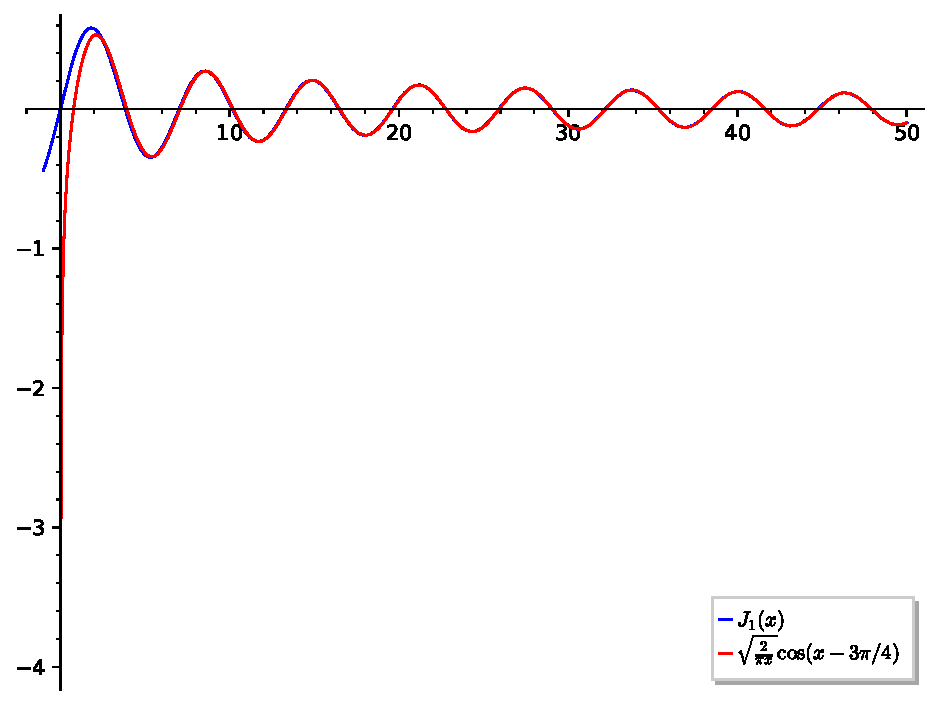
\includegraphics[width=\linewidth]{generated/sageplot/image-bessel-approximation-first-kind.pdf}%
\end{image}%
\end{subsectionptx}
%
%
\typeout{************************************************}
\typeout{Subsection  Bessel Functions of the First Kind for Nonnegative Order}
\typeout{************************************************}
%
\begin{subsectionptx}{Bessel Functions of the First Kind for Nonnegative Order}{}{Bessel Functions of the First Kind for Nonnegative Order}{}{}{x:subsection:subsection-bessel-functions-of-the-first-kind-for-nonnegative-order}
Now we try to find a formula for \(J_{\nu}(x)\) assuming \(\nu\geq0\). To do so, we need to make sense of expressions like \((\nu + k)!\). Thankfully, we can do so using the \emph{Gamma function}.%
\begin{definition}{Gamma Function.}{x:definition:definition-gamma-function}%
\index{Gamma function}%
The \terminology{Gamma function} is the function \(\Gamma(x)\) given by%
\begin{equation*}
\Gamma(x) = \int_{0}^{\infty}t^{x-1}e^{-t}\,dt\text{.}
\end{equation*}
%
\end{definition}
An important property of the Gamma function is the following:%
\begin{equation*}
\Gamma(x + 1) = x\Gamma(x)\text{.}
\end{equation*}
If we replace \(x\) with an integer \(n\geq0\), we get%
\begin{equation*}
\Gamma(n + 1) = n!\text{.}
\end{equation*}
It turns out that we can replace \((\nu + k)!\) in \hyperref[x:men:equation-bessel-function-first-kind]{({\xreffont\ref{x:men:equation-bessel-function-first-kind}})} with \(\Gamma(\nu + k + 1)\), giving%
\begin{equation}
J_{\nu}(x) = x^{\nu}\sum_{k\geq0}\frac{(-1)^{k}}{2^{2k + \nu}k!\Gamma(\nu + k + 1)}x^{2k} = \sum_{k\geq0} \frac{(-1)^{k}}{k!\Gamma(\nu + k + 1)}\left(\frac{x}{2}\right)^{2k + \nu}\text{.}\label{x:men:equation-bessel-first-kind-nonnegative-order}
\end{equation}
Note that the asymptotic expansion in \hyperref[x:men:equation-bessel-asymptotic]{({\xreffont\ref{x:men:equation-bessel-asymptotic}})} holds for noninteger \(\nu\) as well.%
\end{subsectionptx}
%
%
\typeout{************************************************}
\typeout{Subsection  General Solution of Bessel's Equation}
\typeout{************************************************}
%
\begin{subsectionptx}{General Solution of Bessel's Equation}{}{General Solution of Bessel's Equation}{}{}{x:subsection:subsection-general-solution-of-bessel-s-equation}
Since \hyperref[x:men:equation-bessel-plugged-in]{({\xreffont\ref{x:men:equation-bessel-plugged-in}})} is second-order, we need a second linearly independent solution to get the general solution. If \(\nu\) is not an integer then we can find the second solution very quickly: \(J_{-\nu}(x)\). However, if \(\nu\) is an integer then it turns out that \(J_{-\nu}(x) = (-1)^{n}J_{\nu}(x)\), and so fails to be linearly independent from \(J_{\nu}\).%
\par
It turns out that a second, linearly independent solution \(Y_{\nu}\) is given as follows:%
\begin{align}
Y_{\nu}(x) \amp = \frac{1}{\sin(\nu\pi)}[J_{\nu}(x)\cos(\nu\pi) - J_{-\nu}(x)]\label{x:mrow:equation-bessel-second-kind-noninteger}\\
Y_{n}(x) \amp = \lim_{\nu\to n}Y_{\nu}(x)\text{.}\label{x:mrow:equation-bessel-second-kind-integer}
\end{align}
%
\end{subsectionptx}
\end{sectionptx}
\end{chapterptx}
  %
%
\typeout{************************************************}
\typeout{Chapter 6 Laplace Transforms}
\typeout{************************************************}
%
\begin{chapterptx}{Laplace Transforms}{}{Laplace Transforms}{}{}{x:chapter:laplace-transforms}
%
%
\typeout{************************************************}
\typeout{Section 6.1 The Laplace Transform}
\typeout{************************************************}
%
\begin{sectionptx}{The Laplace Transform}{}{The Laplace Transform}{}{}{x:section:section-the-laplace-transform}
%
%
\typeout{************************************************}
\typeout{Subsection  Definition and Basic Properties}
\typeout{************************************************}
%
\begin{subsectionptx}{Definition and Basic Properties}{}{Definition and Basic Properties}{}{}{x:subsection:subsection-definition-and-basic-properties}
\begin{example}{Motivating the Laplace Transform.}{x:example:example-motivating-laplace}%
A mass of \SI{1}{\kilogram} is attached to a spring that is held \SI{1}{\meter} to the right of its equilibrium position by a force of \SI{4}{\newton}. Beginning at time \(t=0\), a machine is turned on and applies an external force of \(\cos2t\) to the mass. At time \(t=2\pi\) the machine is turned off and the external force disappears. Let \(x(t)\) be the displacement of the mass at time \(t\). What is an ODE that models the motion of the mass?%
\par\smallskip%
\noindent\textbf{\blocktitlefont Solution}.\hypertarget{g:solution:idp105548781263776}{}\quad{}We can set this up as we did in Chapter 3. By Hooke's Law and Newton's Second Law, we have%
\begin{equation*}
mx''+kx = F_{E}(t)
\end{equation*}
where \(F_{E}\) is the external force at time \(t\). Since \(m = 1\), \(k = 4\) and%
\begin{equation*}
F_{E}(t) = 
\begin{cases}
\cos2t \amp \text{if }0\leq t\lt 2\pi\\
0 \amp\text{if } t\geq2\pi  
\end{cases}
\end{equation*}
the motion of the mass satisfies the ODE%
\begin{equation*}
x''+4x = F_{E}(t).
\end{equation*}
%
\end{example}
For the above example we could try to solve it as we did in Chapter 3: first by finding the complementary solution \(x_{c}\) (which isn't a problem) and then by finding the particular solution \(x_{p}\) corresponding to \(F_{E}\). However, finding \(x_{p}\) will not be possible using our previous methods since the function \(F_{E}\) is not differentiable everywhere (nor continuous everywhere). We would like to develop a method that lets us solve ODEs that involve discontinuous quantities.%
\begin{definition}{The Laplace Transform.}{x:definition:definition-the-laplace-transform}%
Let \(f(t)\) be defined for \(t\geq0\). The \terminology{Laplace transform} of \(f\) is a function \(F(s)\), or \(\mathcal{L}\left\{ f(t) \right\}\), defined by%
\begin{equation*}
F(s) = \mathcal{L}\left\{ f(t) \right\} = \Int{0}{\infty}f(t)e^{-st}\,dt
\end{equation*}
for all values of \(s\) such that \(F(s)\) exists. We often say that \(f(t)\) is in the \terminology{time domain} while \(F(s)\) is in the \terminology{frequency domain}.%
\end{definition}
One reason we care about the Laplace transform is that it lets us deal with solving linear ODEs involving discontinuous functions. This is something we will begin to look at in the next section.%
\begin{example}{Computing a Laplace Transform.}{x:example:example-computing-a-laplace-transform}%
Compute \(\mathcal{L}\left\{ 1 \right\}\).%
\end{example}
\begin{example}{Computing the Laplace of \(t\).}{x:example:example-computing-the-laplace-of-t-}%
Compute the Laplace transform of \(f(t) = t\).%
\par\smallskip%
\noindent\textbf{\blocktitlefont Solution}.\hypertarget{g:solution:idp105548781473952}{}\quad{}We compute the Laplace transform \(F(s)\) using the definition:%
\begin{align*}
F(s) \amp= \Int{0}{\infty}te^{-st}\,dt\\
\amp= \left[-\frac{t}{s}e^{-st}\right]_{0}^{\infty} + \frac{1}{s}\Int{0}{\infty}e^{-st}\,dt \amp\text{using integration by parts}\\
\amp= -\frac{1}{s^{2}}\left[e^{-st}\right]_{0}^{\infty}\\
\amp= \frac{1}{s^{2}}\text{.}
\end{align*}
%
\end{example}
In general,%
\begin{equation*}
\mathcal{L}\left\{t^{n}\right\} = \frac{n!}{s^{n+1}}
\end{equation*}
if \(n\geq0\) is a whole number.%
\par
The Laplace transform is also an example of a \terminology{linear transformation}. In particular, we have the following theorem.%
\begin{theorem}{Linearity of the Laplace Transform.}{}{x:theorem:theorem-linearity-of-the-laplace-transform}%
Let \(a\) and \(b\) be constants and suppose \(f(t)\) and \(g(t)\) are functions with respective Laplace transforms \(F(s)\) and \(G(s)\). Then%
\begin{equation*}
\Laplace{af+bg} = aF(s)+bG(s).
\end{equation*}
%
\end{theorem}
\begin{example}{Computing the Transform of a Polynomial.}{x:example:example-computing-the-transform-of-a-polynomial}%
Compute \(\Laplace{(t-1)^{3}}\).%
\par\smallskip%
\noindent\textbf{\blocktitlefont Solution}.\hypertarget{g:solution:idp105548781482528}{}\quad{}We could use the definition once again, but here's an easier way using the linearity of the Laplace transform. First, note that%
\begin{equation*}
(t-1)^{3} = t^{3} - 3t^{2} +3t - 1
\end{equation*}
so%
\begin{align*}
\Laplace{(t-1)^{3}} \amp= \Laplace{t^{3}-3t^{2}+3t-1}\\
\amp= \Laplace{t^{3}} - 3\Laplace{t^{2}} +3\Laplace{t} - \Laplace{1}\\
\amp= \frac{3!}{s^{4}} - 3\frac{2!}{s^{3}} + 3\frac{1!}{s^{2}} - \frac{0!}{s}\\
\amp= \frac{6}{s^{4}} - \frac{6}{s^{3}} + \frac{3}{s^{2}} - \frac{1}{s}\text{.}
\end{align*}
%
\end{example}
Another benefit is that the Laplace transform works well with some discontinuous functions.%
\begin{example}{The Unit Step Function.}{x:example:example-the-unit-step-function}%
Let \(u(t)\) be the \terminology{unit step function}, which is defined by%
\begin{equation*}
u(t) = 
\begin{cases}
0 \amp\text{ if } t\lt 0  \\
1 \amp\text{ if } t\geq0
\end{cases}
\end{equation*}
Compute \(\Laplace{u(t-3)}\).%
\par\smallskip%
\noindent\textbf{\blocktitlefont Solution}.\hypertarget{g:solution:idp105548781487264}{}\quad{}Note that we are computing a \emph{translation} of the usual unit step function. We still compute \(\Laplace{u(t-3)}\) using the definition of the Laplace transform:%
\begin{align*}
\Laplace{u(t)} \amp= \Int{0}{\infty}u(t)e^{-st}\,dt\\
\amp= \Int{3}{\infty}e^{-st}\,dt \amp\text{ since }u(t-3) \text{ is }0 \text{ for values of }t\lt3\\
\amp= -\frac{1}{s}\left[e^{-st}\right]_{3}^{\infty}\\
\amp= \frac{e^{-3s}}{s}\text{.}
\end{align*}
%
\end{example}
Some other important Laplace transforms are given below:%
\begin{align*}
\Laplace{e^{at}} \amp= \frac{1}{s-a}\\
\Laplace{\sin(\omega t)} \amp= \frac{k}{s^{2}+\omega^{2}}\\
\Laplace{\cos(\omega t)} \amp= \frac{s}{s^{2}+\omega^{2}}\text{.}
\end{align*}
%
\end{subsectionptx}
%
%
\typeout{************************************************}
\typeout{Subsection  The Inverse Laplace Transform; \(s\)-shifting}
\typeout{************************************************}
%
\begin{subsectionptx}{The Inverse Laplace Transform; \(s\)-shifting}{}{The Inverse Laplace Transform; \(s\)-shifting}{}{}{x:subsection:subsection-the-inverse-laplace-transform-m-s--shifting}
An important theorem regarding Laplace transforms is the following:%
\begin{theorem}{Uniqueness of Laplace Transforms.}{}{x:theorem:theorem-uniqueness-of-inverse-laplace}%
Suppose \(f(t)\) and \(g(t)\) have respective Laplace transforms \(F(s)\) and \(G(s)\). If \(F(s) = G(s)\) for all \(s\gt c\) (for some constant \(c\)) and \(f(t)\) and \(g(t)\) are piecewise continuous, then \(f(t) = g(t)\) on the interval \([0,\infty)\).%
\end{theorem}
The previous theorem says that the Laplace transform is unique for continuous functions: two different continuous functions will have two different Laplace transforms. This allows us to talk about taking inverse Laplace transforms.%
\begin{definition}{Inverse Laplace Transform.}{x:definition:definition-inverse-laplace}%
The \terminology{inverse Laplace transform} of a function \(F(s)\), denoted \(\mathcal{L}^{-1}\left\{F(s)\right\}\), is a function \(f(t)\) such that \(\Laplace{f(t)} = F(s)\).%
\end{definition}
Just like the Laplace transform, the inverse Laplace transform is \terminology{linear}.%
\begin{example}{Finding an Inverse Transform.}{x:example:example-finding-inverse-laplace}%
A continuous function \(f(t)\) has Laplace transform%
\begin{equation*}
F(s) = \frac{3s}{s^{2}+5} + \frac{7}{s^{3}}.
\end{equation*}
Find \(f(t)\).%
\par\smallskip%
\noindentWe can find \(f(t)\) by taking the inverse Laplace transform of each term in \(F(s)\):%
\begin{align*}
\iLaplace{\frac{3s}{s^{2}+5}} \amp= 3\iLaplace{\frac{s}{s^{2}+5}} = 3\cos(\sqrt{5}t)\\
\iLaplace{\frac{7}{s^{3}}} \amp= \frac{7}{2!}\iLaplace{\frac{2!}{s^{3}}} = \frac{7}{2}t^{2}\text{.}
\end{align*}
So%
\begin{equation*}
f(t) = 3\cos(\sqrt{5}t)+\frac{7}{2}t^{2}.
\end{equation*}
%
\end{example}
\begin{theorem}{\(s\)-shifting.}{}{x:theorem:theorem--s--shifting}%
Suppose that \(f(t)\) has Laplace transform \(F(s)\), defined for \(s\gt k\) for some \(k\). Then%
\begin{equation*}
\Laplace{e^{at}f(t)} = F(s-a)\qq{or equivalently} \iLaplace{F(s-a)} = e^{at}f(t).
\end{equation*}
In other words, multiplication by an exponential \(e^{at}\) in the \emph{time domain} corresponds to translation by \(a\) in the \emph{frequency domain}.%
\end{theorem}
\begin{example}{Inverse Laplace with Frequency Shifting.}{x:example:example-inverse-laplace-with-frequency-shifting}%
A function \(f(t)\) has Laplace transform%
\begin{equation*}
F(s) = \frac{4}{s^{2}+2s+3}.
\end{equation*}
Find \(f(t)\).%
\par\smallskip%
\noindent\textbf{\blocktitlefont Solution}.\hypertarget{g:solution:idp105548781446816}{}\quad{}We'll start by completing the square on the denominator of \(F(s)\) to see if we can make it look like \((s-a)^{2}+\omega^{2}\) for some \(a,\omega\):%
\begin{equation*}
F(s) = \frac{4}{(s^{2}+2s+1)+3-1} = \frac{4}{(s+1)^{2}+2}.
\end{equation*}
This looks an \emph{awful} lot like the transform of \(\sin(\sqrt{2}t)\). Since we have \((s+1)^{2}\) instead of \(s^{2}\), this tells us that%
\begin{equation*}
f(t) = \frac{4}{\sqrt{2}}e^{-t}\sin(\sqrt{2}t).
\end{equation*}
%
\end{example}
The following Sage cell verifies the computation in \hyperref[x:example:example-inverse-laplace-with-frequency-shifting]{Example~{\xreffont\ref{x:example:example-inverse-laplace-with-frequency-shifting}}}.%
\begin{sageinput}
var('s t') # specify variables
inverse_laplace(4/(s^2 + 2*s + 3), s, t)
\end{sageinput}
\terminology{SUGGESTED PROBLEMS:} 1, 3, 5, 9, 31, 37. 43\end{subsectionptx}
\end{sectionptx}
%
%
\typeout{************************************************}
\typeout{Section 6.2 Transformation of Initial Value Problems}
\typeout{************************************************}
%
\begin{sectionptx}{Transformation of Initial Value Problems}{}{Transformation of Initial Value Problems}{}{}{x:section:section-transformation-of-initial-value-problems}
\begin{theorem}{Laplace Transforms of Derivatives.}{}{x:theorem:theorem-laplace-transforms-of-derivatives}%
Suppose that the function \(f(t)\) is piecewise smooth and that \(F(s) = \Laplace{f(t)}\) exists. Then \(\Laplace{f'(t)}\) exists and%
\begin{equation*}
\Laplace{f'(t)} = s\Laplace{f(t)}-f(0) = sF(s)-f(0).
\end{equation*}
%
\end{theorem}
The above theorem says that differentiation in the ``time domain'' corresponds to multiplication by \(s\) in the ``frequency domain.'' This will be the most useful property of the Laplace transform for us: it will turn differential equations in the time domain into algebraic equations in the frequency domain.%
\begin{example}{Laplace Transform of a Second Derivative.}{x:example:example-laplace-transform-of-a-second-derivative}%
Let \(f(t)\) be piecewise smooth with Laplace transform \(F(s)\). Compute \(\Laplace{f''(t)}\) using \hyperref[x:theorem:theorem-laplace-transforms-of-derivatives]{Theorem~{\xreffont\ref{x:theorem:theorem-laplace-transforms-of-derivatives}}}.%
\par\smallskip%
\noindent\textbf{\blocktitlefont Solution}.\hypertarget{g:solution:idp105548781459744}{}\quad{}By \hyperref[x:theorem:theorem-laplace-transforms-of-derivatives]{Theorem~{\xreffont\ref{x:theorem:theorem-laplace-transforms-of-derivatives}}} we know that%
\begin{equation*}
\Laplace{f'(t)} = sF(s)-f(0).
\end{equation*}
We can apply \hyperref[x:theorem:theorem-laplace-transforms-of-derivatives]{Theorem~{\xreffont\ref{x:theorem:theorem-laplace-transforms-of-derivatives}}} to \(f^\prime(t)\) as well, since it must also be piecewise smooth:%
\begin{align*}
\Laplace{f''(t)} \amp= s\Laplace{f^\prime(t)} - f^\prime(0)\\
\amp= s(sF(s)-f(0)) - f^\prime(0)\\
\amp= s^{2}F(s) - sf(0) - f^\prime(0)\text{.}
\end{align*}
This process can be continued indefinitely. In general,%
\begin{equation*}
\Laplace{f^{(n)}(t)} = s^{n}F(s) - s^{n-1}f(0) - s^{n-2}f^\prime(0) - \cdots -sf^{(n-2)}(0) - f^{(n-1)}(0).
\end{equation*}
This gives us everything we need to start solving ODEs using Laplace transforms.%
\end{example}
\begin{example}{Solving IVPs with Laplace Transforms.}{x:example:example-solving-ivps-with-laplace-transforms}%
Solve the IVP%
\begin{equation*}
x''+8x^\prime+15x = 0 \qq{} x(0) = 2, x^\prime(0) = -3
\end{equation*}
where \(x\) is a function of \(t\).%
\par\smallskip%
\noindent\textbf{\blocktitlefont Solution}.\hypertarget{g:solution:idp105548781399328}{}\quad{}We will solve this by using Laplace transforms. If we set \(X(s) = \Laplace{x(t)}\), then%
\begin{align*}
\Laplace{x'(t)} \amp= sX(s) - 2\\
\Laplace{x''(t)} \amp= s^{2}X(s) - 2s +3\text{.}
\end{align*}
So if we take the Laplace transform of the entire ODE, we get%
\begin{equation*}
\underbrace{s^{2}X(s) - 2s + 3}_{\Laplace{x''}} + \underbrace{8sX(s) - 16}_{\Laplace{8x'}} + 15X(s) = 0
\end{equation*}
which simplifies to%
\begin{equation*}
s^{2}X(s)+8sX(s)+15X(s) = 2s+13.
\end{equation*}
To solve the ODE we need to find \(x(t) = \mathcal{L}^{-1}\{X(s)\}\), so we now solve the above for \(X(s)\) in order to find the inverse Laplace transform. If we do so, we get%
\begin{equation*}
X(s) = \frac{2s+13}{s^{2}+8s+15} = \frac{2s+13}{(s+3)(s+5)}.
\end{equation*}
This doesn't look like the Laplace transform of anything we know at the moment, but we can simplify the right hand side using partial fractions. If we do so, we get%
\begin{equation*}
X(s) = \frac{\frac{7}{2}}{s+3} - \frac{\frac{3}{2}}{s+5}.
\end{equation*}
So%
\begin{align*}
x(t) \amp= \frac{7}{2}\mathcal{L}^{-1}\left\{\frac{1}{s+3}\right\} - \frac{3}{2}\mathcal{L}^{-1}\left\{\frac{1}{s+5}\right\}\\
\amp= \frac{7}{2}e^{-3t} - \frac{3}{2}e^{-5t}\text{.}
\end{align*}
%
\end{example}
\begin{example}{Nonhomogeneous IVPs with Laplace Transforms.}{x:example:example-nonhomogeneous-ivps-with-laplace-transforms}%
Solve the IVP given by%
\begin{equation*}
y''+9y = 10e^{-t},\quad y(0) = y^\prime(0) = 0.
\end{equation*}
%
\par\smallskip%
\noindent\textbf{\blocktitlefont Solution}.\hypertarget{g:solution:idp105548781405344}{}\quad{}We begin by taking the Laplace transform of both sides to get%
\begin{equation*}
s^{2}Y(s) - sy(0) - y^\prime(0) + 9Y(s) = \frac{10}{s+1}
\end{equation*}
or just%
\begin{equation*}
s^{2}Y(s) + 9Y(s) = \frac{10}{s+1}.
\end{equation*}
So%
\begin{equation*}
Y(s) = \frac{10}{(s+1)(s^{2}+9)}.
\end{equation*}
By partial fractions, this becomes%
\begin{equation*}
Y(s) = \frac{1-s}{s^{2}+9} + \frac{1}{s+1} = \frac{1}{s^{2}+9} - \frac{s}{s^{2}+9} + \frac{1}{s+1},
\end{equation*}
so the solution of the ODE is%
\begin{align*}
y(t) \amp = \iLaplace{Y(s)}\\
\amp= \frac{1}{3}\sin3t -\cos3t + e^{-t}\text{.}
\end{align*}
%
\end{example}
\begin{sageinput}
Y(s) = 10/((s+1) * (s^2+9))
Y(s).partial_fraction_decomposition()
\end{sageinput}
One restriction of the Laplace transform approach as we've developed it is that it requires initial conditions at \(t=0\). If initial conditions are instead given at some other \(t=t_0\), then we need to adjust our approach in order to continue to use \hyperref[x:theorem:theorem-laplace-transforms-of-derivatives]{Theorem~{\xreffont\ref{x:theorem:theorem-laplace-transforms-of-derivatives}}} and its counterpart for second derivatives. We'll demonstrate this by example.%
\begin{example}{Solving an IVP with Shifted Initial Conditions.}{x:example:example-solving-an-ivp-with-shifted-initial-conditions}%
Solve the IVP given by%
\begin{equation*}
y'' - 2y^\prime - 3y = 0\text{ where }y(4) = -3, y^\prime(4) = -17.
\end{equation*}
%
\par\smallskip%
\noindent\textbf{\blocktitlefont Solution}.\hypertarget{g:solution:idp105548781411360}{}\quad{}We would like to take the Laplace transform of both sides of this ODE, but since the initial conditions are not specified at \(0\) we can't do so right away. The trick here is to shift the initial conditions \emph{back} to \(0\) as follows. First, we define a new function \(\widetilde{y}\) by%
\begin{equation*}
\widetilde{y}(t) = y(t+4)
\end{equation*}
where \(y(t)\) is the solution we seek. Then it follows that%
\begin{equation*}
\widetilde{y}'' - 2\widetilde{y}^\prime - 3\widetilde{y} = 0
\end{equation*}
and \(\widetilde{y}(0) = y(4) = -3\) and \(\widetilde{y}^\prime(0) = y^\prime(4) = -17\). So the Laplace transform method applies to solving for \(\widetilde{y}\) in this modified IVP.%
\par
Now that we can take the Laplace transform of both sides of the modified IVP, we do so and obtain the Laplace transform \(\widetilde{Y}(s)\) of \(\widetilde{y}(t)\). Using our initial conditions and a bit of algebra, we get%
\begin{equation*}
\widetilde{Y}(s) = \frac{-11s-3s}{s^2-2s-3}.
\end{equation*}
At this point we can take the inverse Laplace transform (either using partial fractions or using technology) to get%
\begin{equation*}
\widetilde{y}(t) = -5e^{3t} + 2e^{-t}.
\end{equation*}
%
\par
The final step is to convert our answer from \(\widetilde{y}\) to \(y\) by making the substitution \(t\mapsto t-4\) in \(\widetilde{y}\). This gives%
\begin{equation*}
y(t) = -5e^{3(t-4)} + 2e^{-(t-4)}
\end{equation*}
as the solution of our IVP.%
\end{example}
\terminology{SUGGESTED PROBLEMS:} 3-9 odd\end{sectionptx}
%
%
\typeout{************************************************}
\typeout{Section 6.3 Unit Step Functions and Time Shifting}
\typeout{************************************************}
%
\begin{sectionptx}{Unit Step Functions and Time Shifting}{}{Unit Step Functions and Time Shifting}{}{}{x:section:section-unit-step-functions-and-time-shifting}
The \terminology{unit step function} or \terminology{Heaviside function} is the function \(u(t)\) defined by%
\begin{equation*}
u(t) = \begin{cases}
0, \amp\text{ if }t\lt 0\\
1 \amp\text{ if } t\geq0
\end{cases}.
\end{equation*}
Note also that%
\begin{equation*}
u(t-a) = \begin{cases}
0 \amp\text{ if }t\lt a\\
1 \amp\text{ if } t\geq a
\end{cases}
\end{equation*}
for any \(a\).%
\par
Recall that \hyperref[x:theorem:theorem--s--shifting]{Theorem~{\xreffont\ref{x:theorem:theorem--s--shifting}}} tells us how to deal with translation in the frequency domain:%
\begin{equation*}
\Laplace{e^{at}f(t)} = F(s-a) \quad\text{or}\quad\iLaplace{F(s-a)} = e^{at}f(t).
\end{equation*}
A similar result is true for \(t\)-shifting.%
\begin{theorem}{Time Shifting of Laplace Transforms.}{}{x:theorem:theorem-time-shifting-of-laplace-transforms}%
Let \(f(t)\) denote a piecewise continuous function with Laplace transform \(F(s)\). Let \(a\geq0\). Then \(\Laplace{u(t-a)f(t-a)} = e^{-as}F(s)\), or equivalently \(\iLaplace{e^{-as}F(s)} = u(t-a)f(t-a)\).%
\end{theorem}
\begin{proof}{}{g:proof:idp105548781428256}
To compute this we need to rely on the definition of the Laplace transform:%
\begin{align*}
\Laplace{u(t-a)f(t-a)} \amp= \int_{0}^{\infty}u(t-a)f(t-a)e^{-st}\,dt\\
\amp= \int_{a}^{\infty}f(t-a)e^{-st}\,dt\\
\amp= \int_{0}^{\infty}f(\tau)e^{-s(\tau+a)}\,d\tau\\
\amp= e^{-sa}\int_{0}^{\infty}f(\tau)e^{-s\tau}\,d\tau\\
\amp= e^{-as}F(s)\text{.}\qedhere
\end{align*}
%
\end{proof}
The Heaviside function is useful for describing forces that turn on or off at specified times. In particular, we can now solve the IVP given at the start of this chapter in \hyperref[x:example:example-motivating-laplace]{Example~{\xreffont\ref{x:example:example-motivating-laplace}}}.%
\begin{example}{IVP with Discontinuous Forcing Function.}{x:example:example-ivp-with-discontinuous-forcing-function}%
A mass of \SI{1}{\kilogram} is attached to a spring that is held \SI{1}{\meter} to the right of its equilibrium position by a force of \SI{4}{\newton}. Beginning at time \(t=0\), a machine is turned on and applies an external force of \(\cos2t\) to the mass. At time \(t=2\pi\) the machine is turned off and the external force disappears. Let \(x(t)\) be the displacement of the mass at time \(t\). What is an ODE that models the motion of the mass?%
\par\smallskip%
\noindent\textbf{\blocktitlefont Solution}.\hypertarget{g:solution:idp105548781370272}{}\quad{}By Hooke's Law and Newton's Second Law, we have%
\begin{equation*}
mx''+kx = F_{E}(t)
\end{equation*}
where \(F_{E}\) is the external force at time \(t\). Since \(m = 1\), \(k = 4\) and%
\begin{equation*}
F_{E}(t) = 
\begin{cases}
\cos3t \amp\text{if }0\leq t\lt 2\pi\\
0 \amp\text{if }t\geq2\pi  
\end{cases}
\end{equation*}
the motion of the mass satisfies the IVP%
\begin{equation*}
x''+4x = F_{E}(t), x(0) = 1, x^\prime(0) = 0.
\end{equation*}
We can rewrite \(F_{E}(t)\) as follows:%
\begin{equation*}
F_{E}(t) = [u(t-0)-u(t-2\pi)]\cos3t = u(t)\cos3t - u(t-2\pi)\cos3t.
\end{equation*}
So the IVP we need to solve is%
\begin{equation*}
x''+4x = u(t)\cos3t - u(t-2\pi)\cos3t, x(0) = 1, x^\prime(0) = 0.
\end{equation*}
%
\par
If we take Laplace transforms, this becomes%
\begin{equation*}
s^{2}X(s) - s + 4X(s) = \Laplace{F_{E}(t)},
\end{equation*}
where%
\begin{align*}
\Laplace{F_{E}(t)} \amp= \Laplace{u(t)\cos3t} - \Laplace{u(t-2\pi)\cos3t}\\
\amp= \frac{s}{s^{2}+9} - \Laplace{u(t-2\pi)\cos(3(t-2\pi)+6\pi)}\\
\amp= \frac{s}{s^{2}+9} - \Laplace{u(t-2\pi)\cos(3(t-2\pi))}\\
\amp= \frac{s}{s^{2}+9} - e^{-2\pi s}\frac{s}{s^{2}+9}\text{.}
\end{align*}
So%
\begin{equation*}
s^{2}X(s) - s + 4X(s) = \frac{s}{s^{2}+9} - e^{-2\pi s}\frac{s}{s^{2}+9}.
\end{equation*}
If we solve this for \(X(s)\), we get%
\begin{equation*}
X(s) = \frac{s}{s^{2}+4} + \frac{s}{(s^{2}+9)(s^{2}+4)} - e^{-2\pi s}\frac{s}{(s^{2}+9)(s^{2}+4)},
\end{equation*}
and if we simplify this using partial fractions this becomes%
\begin{equation*}
X(s) = \frac{s}{s^{2}+4} + \frac{1}{5}\left[\frac{s}{s^{2}+4} - \frac{s}{s^{2}+9}\right]\parens{1-e^{-2\pi s}}.
\end{equation*}
%
\par
So the solution of the IVP is%
\begin{align*}
x(t) \amp= \iLaplace{\frac{s}{s^{2}+4} + \frac{1}{5}\left[\frac{s}{s^{2}+4} - \frac{s}{s^{2}+9}\right]\parens\left(1-e^{-2\pi s}}\right)\\
\amp= \cos2t + \frac{1}{5}\left(\cos2t-\cos3t\right) - \frac{1}{5}\left(u(t-2\pi)\cos[2(t-2\pi)] - u(t-2\pi)\cos[3(t-2\pi)]\right)\text{.}
\end{align*}
%
\end{example}
Although it's important to know how to deal with Laplace transforms of basic functions by hand, if only to understand the behavior of the transform itself in solving differential equations, computing transforms of more complicated functions or piecewise functions like the function in \hyperref[x:example:example-ivp-with-discontinuous-forcing-function]{Example~{\xreffont\ref{x:example:example-ivp-with-discontinuous-forcing-function}}} are perhaps better left to computer systems. The code cell below demonstrates how Sage can compute such a transform. \alert{Be careful to place matching brackets and parentheses as appropriate} when using the \mono{piecewise} command in Sage to construct a piecewise function.%
\begin{sageinput}
# declare meaningful variables for Laplace transform
var('s t')

# define piecewise function using piecewise()
# piecewise() command uses a list of cases separated by commas to construct its function
# add more cases if needed
case1 = ((0, 2*pi), cos(3*t))
case2 = ((2*pi, oo), 0)
F_E = piecewise([case1, case2])

# now we can compute the Laplace transform using the .laplace() method
# the arguments (t,s) tell Sage to change from t to s after computing the transform
F_E.laplace(t,s)
\end{sageinput}
\terminology{SUGGESTED PROBLEMS:} 5, 9, 13, 17, 19, 21 odd\end{sectionptx}
%
%
\typeout{************************************************}
\typeout{Section 6.4 Dirac Delta Functions}
\typeout{************************************************}
%
\begin{sectionptx}{Dirac Delta Functions}{}{Dirac Delta Functions}{}{}{x:section:section-dirac-delta-functions}
%
%
\typeout{************************************************}
\typeout{Subsection  Impulses}
\typeout{************************************************}
%
\begin{subsectionptx}{Impulses}{}{Impulses}{}{}{x:subsection:subsection-impulses}
Forces that act over very short time intervals may be complicated to describe exactly, but it we can approximate such a force if we treat it as instantaneous. Our goal now is describe a meaningful mathematical interpretation of an instantaneous force.%
\par
To be specific, let \(f(t)\) be a force that acts only from \(t=a\) to \(t=b\) (and is otherwise \(0\)). Then the \terminology{impulse} of the force \(f(t)\) over the interval \([a,b]\) is given by%
\begin{equation*}
p = \Int{a}{b}f(t)\dd{t}.
\end{equation*}
We view the impulse as essentially describing how the force acts over a short time interval, so we can switch from modeling instantaneous forces to instantaneous impulses. And since the impulse is a number, all we really need to do is model an instantaneous \emph{unit impulse}; any other impulse we can get by multiplication by a constant.%
\par
So this is our goal: find some function \(d(t)\) that has an instantaneous unit impulse at the point \(t=0\). In other words, we want to find a function \(d(t)\) such that%
\begin{equation*}
\int_{0}^{0}d(t)\,dt = 1
\end{equation*}
But this is impossible for any function, since%
\begin{equation*}
\Int{0}{0}d(t)\dd{t} = 0.
\end{equation*}
However, we can approximate the \emph{idea} of an instantaneous unit impulse by defining%
\begin{equation*}
d_{\varepsilon}(t) = 
\begin{cases}
\frac{1}{\varepsilon} \amp\text{if }-\frac{\varepsilon}{2}\leq t\leq \frac{\varepsilon}{2} \\
0 \amp\text{otherwise}  
\end{cases}.
\end{equation*}
\begin{figureptx}{Approximating the instantaneous unit impulse.}{x:figure:figure-approximation-unit-impulse}{}%
\begin{image}{0}{1}{0}%
\resizebox{\linewidth}{!}{%
\begin{tikzpicture}[scale=0.7]
\begin{axis}[
ticks = none,
enlargelimits=false,
legend cell align=left,
axis x line = middle,
xlabel = $t$,
axis y line = center,
ymin = -.5,
ymax = 1.5
]
\addplot[domain=-.5:.5,thick,samples=200,blue]{1};
\addplot[domain=-2.5:-.5,thick,samples=200,blue]{0};
\addplot[domain=.5:2.5,thick,samples=200,blue]{0};
\addlegendentry{$d_{\varepsilon}(t)$}
\end{axis}
\end{tikzpicture}
}%
\end{image}%
\tcblower
\end{figureptx}%
%
\par
Then for any \(\varepsilon\), we have%
\begin{equation*}
\Int{-\frac{\varepsilon}{2}}{\frac{\varepsilon}{2}}d_{\varepsilon}(t)\dd{t} = 1.
\end{equation*}
\(d_{\varepsilon}(t)\) is a completely valid function, and if we send \(\varepsilon\to0\) then it becomes a better and better approximation to an instantaneous unit impulse. Despite the fact that this limit does not exist (at least in the usual sense), we use it as a definition.%
\begin{definition}{The Dirac Delta Function.}{x:definition:definition-dirac-delta}%
The \terminology{Dirac delta function}, denoted by the symbol \(\delta(t)\), is ``defined'' by the equation%
\begin{equation*}
\delta(t) = \limit{\varepsilon}{0}d_{\varepsilon}(t).
\end{equation*}
%
\end{definition}
The Dirac delta function is, of course, not an actual function. \begin{aside}{}{g:aside:idp105548781396000}%
The Dirac delta is actually an example of a \terminology{generalized function}, or \terminology{tempered distribution}.%
\end{aside}
 But it's still useful as a mathematical formulation of an instantaneous force with unit impulse at \(t=0\).%
\par
We can also take translations of the Dirac delta, which we view as a ``function'' \(\delta(t-a)\) defined piecewise by%
\begin{equation*}
\delta(t-a)=
\begin{cases}
\infty \amp\text{if }t=a\\
0 \amp\text{if }t\neq a
\end{cases}.
\end{equation*}
We represent this graphically as an arrow: \begin{figureptx}{A plot of the Dirac delta function.}{g:figure:idp105548781595424}{}%
\begin{image}{0}{1}{0}%
\resizebox{\linewidth}{!}{%
\begin{tikzpicture}
\draw (-3,0)--(3,0);
\draw[->,ultra thick, blue] (0,0)--(0,1) node[above,black]{$\delta(t)$};
\draw[->,ultra thick, blue] (2.5,0)--(2.5,1) node[above,black]{$\delta(t-a)$};
\node at (0,0) [below]{$t=0$};
\node at (2.5,0) [below]{$t=a$};
\end{tikzpicture}
}%
\end{image}%
\tcblower
\end{figureptx}%
%
\par
The most important property of the Dirac delta is that%
\begin{equation*}
\Int{\alpha}{\beta}\delta(t-a)\dd{t} = 
\begin{cases}
1 \amp\text{if }\alpha\leq a\leq\beta \\
0 \amp\text{otherwise.}  
\end{cases}
\end{equation*}
%
\par
We also have the important theorem formula for continuous functions.%
\begin{theorem}{Sifting Property.}{}{x:theorem:theorem-sifting-property}%
Let \(g(t)\) be a continuous function and let \(\alpha\leq a\leq\beta\). Then%
\begin{equation*}
\Int{\alpha}{\beta}g(t)\delta(t-a)\dd{t} = g(a)
\end{equation*}
%
\end{theorem}
\begin{proof}{}{g:proof:idp105548781599392}
We treat \(\delta(t)\) as a function and perform the above integration:%
\begin{align*}
\end{align*}
%
\end{proof}
The above theorem gives us another interpretation of the Dirac delta: it's a ``sampling function''. When integrated against another function \(g(t)\) over an interval containing \(a\), \(\delta(t-a)\) will pick out the value \(g(a)\). We can use this to find the Laplace transform of the Dirac delta.%
\begin{example}{Laplace Transform of the Dirac Delta Function.}{x:example:example-laplace-transform-of-the-dirac-delta-function}%
Compute \(\Laplace{\delta(t-a)}\), where \(a\geq0\).%
\par\smallskip%
\noindent\textbf{\blocktitlefont Solution}.\hypertarget{g:solution:idp105548781604384}{}\quad{}We use the definition of the Laplace transform:%
\begin{align*}
\Laplace{\delta(t-a)} \amp= \int_{0}^{\infty}\delta(t-a)e^{-st}\,dt\\
\amp= e^{-as}\text{.}
\end{align*}
In particular, \(\Laplace{\delta(t)} = 1\).%
\end{example}
\end{subsectionptx}
%
%
\typeout{************************************************}
\typeout{Subsection  Dirac Delta Models}
\typeout{************************************************}
%
\begin{subsectionptx}{Dirac Delta Models}{}{Dirac Delta Models}{}{}{x:subsection:subsection-dirac-delta-models}
We use the Dirac delta to model instantaneous forces, such as sudden kicks or jolts.%
\begin{example}{IVP with Impulse.}{x:example:example-ivp-with-impulse}%
An object of mass \(m=1\), at rest, is attached to a spring with spring constant \(k=9\). At time \(t=0\), the a hammer strikes the mass providing an impulse of \(3\) and setting the mass in motion. What is the displacement \(x(t)\)?%
\par\smallskip%
\noindent\textbf{\blocktitlefont Solution}.\hypertarget{g:solution:idp105548781609888}{}\quad{}\(x(t)\) satisfies the ODE%
\begin{equation*}
mx''+kx = f(t)
\end{equation*}
where \(f(t)\) is the external force. Since the hammer strikes quickly, we can model it as an instantaneous force of the form \(c\delta(t)\). And since it provides an impulse of \(3\), we can pick \(f(t) = 3\delta(t)\). As the mass is initially at rest, \(x\) satisfies the IVP%
\begin{equation*}
x''+9x = 3\delta(t)\qq{where}x(0) = x'(0) = 0.
\end{equation*}
To solve this, we take the Laplace transform of the IVP to get%
\begin{equation*}
s^{2}X(s)+9X(s) = 3
\end{equation*}
or just%
\begin{equation*}
X(s) = \frac{3}{s^{2}+9}.
\end{equation*}
So \(x(t) = \sin3t\).%
\end{example}
Note that the above solution does not appear to satisfy our initial conditions. However, since we assumed the impulse acted instantaneously at time \(t=0\), this is really the same as assuming that the mass had an initial velocity. Now we look at what happens if we delay the hammer strike.%
\begin{example}{Time-delayed Strike.}{x:example:example-time-delay}%
Consider the spring-mass system above, but suppose now that the hammer hits the mass at time \(t=4\). What is the displacement \(x(t)\)?%
\par\smallskip%
\noindent\textbf{\blocktitlefont Solution}.\hypertarget{g:solution:idp105548781616928}{}\quad{}This time, the IVP we must solve is%
\begin{equation*}
x''+9x = 3\delta(t-4)\qq{where}x(0)=x'(0)=0.
\end{equation*}
If we take Laplace transforms and solve for \(X(s)\) we get%
\begin{equation*}
X(s) = \frac{3e^{-4s}}{s^{2}+9}
\end{equation*}
and so, using our table, we see that%
\begin{equation*}
x(t) = u(t-4)\sin[3(t-4)].
\end{equation*}
%
\end{example}
\begin{figureptx}{}{x:figure:figure-time-delay}{}%
\begin{image}{0}{1}{0}%
\resizebox{\linewidth}{!}{%
\begin{tikzpicture}[scale=0.7]
\begin{axis}[
enlargelimits=false,
legend cell align=left,
axis x line = middle,
xlabel = $t$,
xmin = -1,
axis y line = center
]
\addplot[domain=0:4,thick,samples=200,blue]{0};
\addplot[domain=4:9,thick,samples=200,blue]{sin(deg(3*x-12))};
\addlegendentry{$x(t)$}
\end{axis}
\end{tikzpicture}
}%
\end{image}%
\tcblower
\end{figureptx}%
\begin{example}{Resonance with an Impulse Train.}{x:example:example-resonance-with-an-impulse-train}%
Once again we consider the spring-mass system used above, but now we suppose that the mass is struck with the hammer once every \(\frac{2\pi}{3}\) seconds, starting at \(t=0\). Find \(x(t)\).%
\par\smallskip%
\noindent\textbf{\blocktitlefont Solution}.\hypertarget{g:solution:idp105548781622304}{}\quad{}The IVP we need to solve now is%
\begin{align*}
x''+9x \amp= 3\delta(t)+3\delta(t-\frac{2\pi}{3}) + 3\delta(t-\frac{4\pi}{3}) +\cdots\\
\amp= 3\Sum{n=0}{\infty}\delta(t-\frac{2\pi n}{3})
\end{align*}
where \(x(0) = x'(0) = 0\). So once more we take Laplace transforms to get%
\begin{equation*}
s^{2}X(s)+9X(s) = 3\Sum{n=0}{\infty}\Laplace{\delta(t-\frac{2\pi n}{3})} = 3\Sum{n=0}{\infty}e^{-\frac{2\pi n}{3}s}
\end{equation*}
and so%
\begin{equation*}
X(s) = \frac{3}{s^{2}+9}\Sum{n=0}{\infty}e^{-\frac{2\pi n}{3}s}
\end{equation*}
The displacement is then given by%
\begin{align*}
x(t) \amp= \iLaplace{X(s)}\\
\amp= \iLaplace{\frac{3}{s^{2}+9}\cdot\Sum{n=0}{\infty}e^{-\frac{2\pi n}{3}s}}\\
\amp= \iLaplace{\Sum{n=0}{\infty}e^{-\frac{2\pi n}{3}}\frac{3}{s^{2}+9}}\\
\amp= \Sum{n=0}{\infty}u(t-\frac{2\pi n}{3})\sin[3(t-\frac{2\pi n}{3})]\\
\amp= \Sum{n=0}{\infty}u(t-\frac{2\pi n}{3})\sin3t\text{.}
\end{align*}
Each time the hammer strikes the mass, a factor of \(\sin3t\) is added to the displacement. The repeated hammer strikes are in tune with the natural frequency of the mass, so they create resonance.%
\end{example}
\begin{figureptx}{}{x:figure:figure-impulse-train-resonance}{}%
\begin{image}{0}{1}{0}%
\resizebox{\linewidth}{!}{%
\begin{tikzpicture}[scale = .7]
\begin{axis}[
enlargelimits=false,
legend cell align=left,
axis x line = middle,
xlabel = $t$,
ylabel = $x$,
axis y line = center
]
\addplot[domain=0:2*pi/3,thick,samples=200,blue]{sin(deg(3*x))};
\addplot[domain=2*pi/3:4*pi/3,thick,samples=200,blue]{2*sin(deg(3*x))};
\addplot[domain=4*pi/3:6*pi/3,thick,samples=200,blue]{3*sin(deg(3*x))};
\addplot[domain=6*pi/3:8*pi/3,thick,samples=200,blue]{4*sin(deg(3*x))};
\addlegendentry{$x(t)$}
\end{axis}
\end{tikzpicture}
}%
\end{image}%
\tcblower
\end{figureptx}%
\end{subsectionptx}
\terminology{SUGGESTED PROBLEMS:} 3, 7\end{sectionptx}
%
%
\typeout{************************************************}
\typeout{Section 6.5 Convolution Products}
\typeout{************************************************}
%
\begin{sectionptx}{Convolution Products}{}{Convolution Products}{}{}{x:section:section-convolution-products}
Consider the function \(F(s)\) in the frequency domain \(s\) defined by%
\begin{equation*}
F(s) = \frac{1}{s(s^{2}+4)}.
\end{equation*}
This does not match a Laplace transform on our table. If we wanted to find the inverse transform \(f(t)\), we would have to use partial fractions to find it. However, \(F(s)\) is easily seen to be the \emph{product} of two recognizable transforms:%
\begin{equation*}
F(s) = \frac{1}{s} \frac{1}{s^{2}+4} = \frac{1}{2}\Laplace{1}\Laplace{\sin2t}.
\end{equation*}
What we would like to do is find a way to determine inverse transforms of products of transforms. To do this, we need to define the \emph{convolution} of two functions.%
\begin{definition}{Convolution of Functions.}{x:definition:definition-convolution-of-functions}%
Let \(f\) and \(g\) be piecewise continuous functions. The \terminology{convolution} of \(f\) and \(g\), denoted by \((f\ast g)(t)\), \(f(t)\ast g(t)\) or just \(f\ast g\), is defined for \(t\geq0\) by%
\begin{equation*}
(f\ast g)(t) = \Int{0}{t} f(\tau)g(t-\tau)\,d\tau.
\end{equation*}
The variable \(\tau\) is a dummy variable.%
\end{definition}
Note that \(f\ast g\) lies in the time domain instead of the frequency domain. In general, we will only take convolutions of functions in the time domain.%
\par
Convolutions are important because they act as ``smoothing operators''. If you have a ``rough'' (i.e. non-differentiable) function, then convolving it with a properly chosen smooth function may give you a smooth approximation.%
\begin{example}{Convolution with Unit Step.}{x:example:example-convolution-with-unit-step}%
Compute \(u\ast t\), where \(u(t)\) is the unit step function.%
\par\smallskip%
\noindent\textbf{\blocktitlefont Solution}.\hypertarget{g:solution:idp105548781576224}{}\quad{}By definition,%
\begin{align*}
u(t)\ast t \amp= \Int{0}{t}u(\tau)(t-\tau)\,d\tau \\
\amp= \Int{0}{t}(t-\tau)\,d\tau \\
\amp= \left[t\tau-\frac{\tau^{2}}{2}\right]_{\tau=0}^{\tau=t} \\
\amp= \frac{t^{2}}{2}
\end{align*}
%
\end{example}
One important property of convolutions is that they are \emph{commutative}: that is, \(f\ast g = g\ast f\) for any piecewise continuous functions \(f\) and \(g\). Another important property of convolutions is that they tend to work well with integral transforms. In particular, we have the following theorem.%
\begin{theorem}{Convolution Theorem.}{}{x:theorem:theorem-convolution-transform}%
The Laplace transform distributes over convolution. In other words, if \(f\) and \(g\) are piecewise continuous functions, then%
\begin{equation*}
\Laplace{f(t)\ast g(t)} = \Laplace{f(t)}\Laplace{g(t)}.
\end{equation*}
Equivalently, if we write \(F(s) = \Laplace{f(t)}\) and \(G(s) = \Laplace{g(t)}\), then%
\begin{equation*}
\iLaplace{F(s)G(s)} = f(t)\ast g(t) = \Int{0}{t}f(\tau)g(t-\tau).
\end{equation*}
%
\end{theorem}
One way to phrase the above result is that Laplace transforms turns convolution in the time domain into multiplication in the frequency domain. Let's return to the example we started with.%
\begin{example}{Using the Convolution Theorem.}{x:example:example-using-the-convolution-theorem}%
Let%
\begin{equation*}
F(s) = \frac{1}{s(s^{2}+4)}.
\end{equation*}
Find \(f(t) = \iLaplace{F(s)}\).%
\par\smallskip%
\noindent\textbf{\blocktitlefont Solution}.\hypertarget{g:solution:idp105548781584288}{}\quad{}We will use \hyperref[x:theorem:theorem-convolution-transform]{Theorem~{\xreffont\ref{x:theorem:theorem-convolution-transform}}} to express the inverse transform:%
\begin{align*}
f(t) \amp= \iLaplace{F(s)}\\
\amp= \iLaplace{\frac{1}{s}\cdot\frac{1}{s^{2}+4}}\\
\amp= 1\ast \frac{1}{2}\sin2t\\
\amp= \frac{1}{2}\Int{0}{t}\sin2\tau\,d\tau\\
\amp= -\frac{1}{4}\left[\cos2\tau\right]_{\tau=0}^{\tau=t}\\
\amp= \frac{1-\cos2t}{4}
\end{align*}
%
\end{example}
\begin{example}{Solving IVPs with the Convolution Theorem.}{x:example:example-solving-ivps-with-the-convolution-theorem}%
Let \(x\) be a function of \(t\). Solve the IVP%
\begin{equation*}
x''+4x'+13x = f(t)\qq{where}x(0) = x'(0) = 0
\end{equation*}
for \(x(t)\) in terms of the function \(f(t)\).%
\par\smallskip%
\noindent\textbf{\blocktitlefont Solution}.\hypertarget{g:solution:idp105548781589792}{}\quad{}We're trying to find the solution \(x(t)\) for arbitrary \(f(t)\), which is something we definitely would not have been able to do in Chapter 3. We will do so using Laplace transforms and \hyperref[x:theorem:theorem-convolution-transform]{Theorem~{\xreffont\ref{x:theorem:theorem-convolution-transform}}}. So we start by taking the Laplace transform of the ODE to get%
\begin{equation*}
s^{2}X(s) +4sX(s) + 13X(s) = F(s)
\end{equation*}
where \(X(s) = \Laplace{x(t)}\) and \(F(s) = \Laplace{f(t)}\). Now we solve for \(X(s)\) to get%
\begin{equation*}
X(s) = \frac{F(s)}{s^{2}+4s+13} = F(s)G(s)
\end{equation*}
where%
\begin{equation*}
G(s) = \frac{1}{s^{2}+4s+13}
\end{equation*}
\hyperref[x:theorem:theorem-convolution-transform]{Theorem~{\xreffont\ref{x:theorem:theorem-convolution-transform}}} tells us then that%
\begin{equation*}
x(t) = \iLaplace{F(s)G(s)} = f(t)*g(t)
\end{equation*}
where%
\begin{align*}
g(t) \amp= \iLaplace{G(s)}\\
\amp= \iLaplace{\frac{1}{s^{2}+4s+13}} \\
\amp= \iLaplace{\frac{1}{(s+2)^{2}+9}} \amp \text{complete the square}\\
\amp= \frac{1}{3}e^{-2t}\sin3t \amp \text{use a translation formula}
\end{align*}
Therefore the solution of the ODE in terms of the function \(f(t)\) is given by%
\begin{align*}
x(t) \amp= f(t)\ast g(t)\\
\amp= \Int{0}{t}f(\tau)g(t-\tau)\,d\tau\\
\amp= \int_{0}^{t}f(\tau)\frac{e^{-2(t-\tau)}\sin[3(t-\tau)]}{3}\,d\tau\text{.}
\end{align*}
%
\end{example}
There are a couple of interesting things happening in the last example. In particular, we were able to write the solution \(x(t)\) in terms of \(f(t)\) as%
\begin{equation*}
x(t) = g(t)\ast f(t)\text{.}
\end{equation*}
In these terms, we can view \(f(t)\) as the input into a particular system (whose behavior is determined by the ODE) and the solution \(x(t)\) is the corresponding output. This relationship is even easier to write in the frequency domain: the frequency input \(F(s)\) is turned into the frequency output \(X(s)\) by means of the \terminology{transfer function} \(G(s)\):%
\begin{equation*}
X(s) = G(s)F(s)\text{.}
\end{equation*}
%
\par
The importance of the transfer function in applications is that it encodes \emph{all possible outputs} the system is capable of producing. There are multiple ways to find the transfer function, assuming that all initial conditions are \(0\). First, if \(F(s)\) is the input and \(X(s)\) is some measured output (once again, in the frequency domain), then the transfer function \(G(s)\) satisfies%
\begin{equation*}
G(s) = \frac{X(s)}{F(s)}\text{,}
\end{equation*}
and this quantity is independent of the particular choice of \(F(s)\). In particular, we can replace the time domain input \(f(t)\) with \(\delta(t)\). In this case, the corresponding output in the frequency domain is%
\begin{equation*}
X(s) = G(s)\Laplace{\delta(t)} = G(s)\text{.}
\end{equation*}
For this reason, the inverse transform of the transfer function is also known as the \terminology{impulse response} of the system.%
\par
\terminology{SUGGESTED PROBLEMS:} 1, 3, 17, 21, 25%
\end{sectionptx}
\end{chapterptx}
 \end{partptx}
%
%
\typeout{************************************************}
\typeout{Part II Partial Differential Equations}
\typeout{************************************************}
%
\begin{partptx}{Partial Differential Equations}{}{Partial Differential Equations}{}{}{x:part:part-pdes}
 %
%
\typeout{************************************************}
\typeout{Chapter 7 Fourier Analysis}
\typeout{************************************************}
%
\begin{chapterptx}{Fourier Analysis}{}{Fourier Analysis}{}{}{x:chapter:fourier-analysis}
\begin{introduction}{}%
Our goal now is to move to solving \emph{partial} differential equations (PDEs), which are differential equations that involve multiple independent variables. Such equations are particularly useful for modeling quantities that depend on position \(x\) and time \(t\). It turns out that these partial differential equations often involve periodic functions. So our first step to solving PDEs will be to find useful descriptions of periodic (and in some cases, non-periodic) functions.%
\end{introduction}%
%
%
\typeout{************************************************}
\typeout{Section 7.1 Fourier Series}
\typeout{************************************************}
%
\begin{sectionptx}{Fourier Series}{}{Fourier Series}{}{}{x:section:section-fourier-series}
\begin{introduction}{}%
The main idea behind Fourier series, and the field of harmonic analysis in general, is to represent more complicated objects in terms of simpler objects. A fundamental example of this idea comes from the field of linear algebra in the form of \emph{orthonormal bases}. Knowing an orthonormal basis for a vector space \(V\) can greatly simplify linear algebra in that vector space. In this section, we'll do something similar with periodic functions.%
\end{introduction}%
%
%
\typeout{************************************************}
\typeout{Subsection  Periodic Functions}
\typeout{************************************************}
%
\begin{subsectionptx}{Periodic Functions}{}{Periodic Functions}{}{}{x:subsection:subsection-periodic-functions}
Consider the function \(f(x)\) given by the following graph:%
\begin{figureptx}{A periodic function.}{x:figure:figure-sageplot-periodic-function}{}%
\begin{image}{0}{1}{0}%
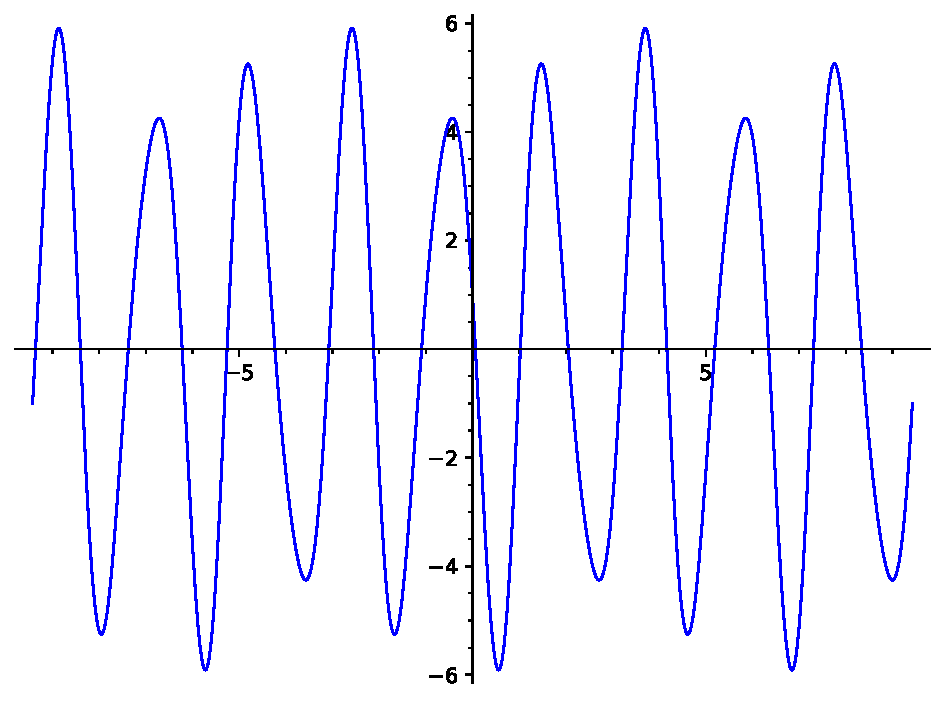
\includegraphics[width=\linewidth]{generated/sageplot/image-sageplot-periodic-function.pdf}%
\end{image}%
\tcblower
\end{figureptx}%
This function can be plotted using the following code:%
\begin{sageinput}
import matplotlib.pyplot as plt
import numpy as np

# This is setting up our graph.
x = np.linspace(-3*np.pi,3*np.pi,200)
y1 = np.cos(5*x)
y2 = np.sin(3*x)

# This actually plots the graph.
p = plt.plot(x, y1 - 5*y2, label=r'$f(x)$')
plt.legend()
plt.show()
\end{sageinput}
If we look at the graph, we see that it repeats itself if we wait long enough. Functions that have this property are called \terminology{periodic functions}.%
\begin{definition}{Periodic Functions.}{x:definition:definition-periodic-functions}%
\index{Functions!periodic}%
Let \(f(x)\) be a real function defined for all \(x\). We say that \(f\) is a periodic function if there exists a positive number \(p\) such that%
\begin{equation*}
f(x+p) = f(x)
\end{equation*}
for all \(x\).%
\end{definition}
 Let \(n\) be any integer. Then the functions \(\sin nx\) and \(\cos nx\) are both periodic and have period \(2\pi\) since%
\begin{align*}
\sin[n(x+2\pi)] \amp = \sin nx\cos2\pi + \cos nx\sin2\pi = \sin nx \\
\cos[n(x+2\pi)] \amp = \cos nx\cos2\pi - \sin nx\sin2\pi = \cos nx 
\end{align*}
The periodic nature of these functions can also be seen from their graphs:%
 \begin{sageinput}
# This is setting up our graph.
x = np.linspace(-3*np.pi,3*np.pi,200)
y1 = np.cos(5*x)
y2 = np.sin(2*x)

# This actually plots the graphs.
plt.subplot(2,1,1)
plt.plot(x,y1,label=r'$\cos(5x)$')
plt.legend()

plt.subplot(2,1,2)
plt.plot(x,y2,label=r'$\sin(2x)$')
plt.legend()
plt.show()
\end{sageinput}
If you go back to the first plot, you may notice from the code used to generate the function \(f(x)\) that \(f(x)\) is just the sum of two basic trigonometric functions:%
\begin{equation*}
f(x) = \cos5x-5\sin3x.
\end{equation*}
In other words, the (finite) sum of functions of the form \(\sin nx,\cos mx\) where \(n,m\) are integers is also periodic, and also has period \(2\pi\). One of the greatest accomplishments in mathematics was the realization that many other periodic functions can be written in this way if we allow \emph{infinite} sums of this form, which we call \terminology{trigonometric series}.%
\end{subsectionptx}
%
%
\typeout{************************************************}
\typeout{Subsection  Trigonometric Series and Fourier Series}
\typeout{************************************************}
%
\begin{subsectionptx}{Trigonometric Series and Fourier Series}{}{Trigonometric Series and Fourier Series}{}{}{x:subsection:subsection-trig-and-fourier-series}
\begin{definition}{Trigonometric Series.}{x:definition:definition-trigonometric-series}%
\index{Series!trigonometric}%
A trigonometric series is a series of the form%
\begin{equation*}
\sum_{k=0}^{\infty}(a_{k}\cos kx+b_{k}\sin kx) = a_{0} + \sum_{k=1}^{\infty}(a_{k}\cos kx+b_{k}\sin kx)
\end{equation*}
where \(a_{k},b_{k}\) are constants, called the \terminology{coefficients} of the series.%
\end{definition}
Our primary goal in this section is to take a function \(f(x)\) of period \(2\pi\) and express it as a trigonometric series. To see how, we'll suppose that we have the trigonometric series we want, i.e. that%
\begin{equation*}
f(x) = a_{0} + \sum_{k=1}^{\infty}(a_{k}\cos kx+b_{k}\sin kx),
\end{equation*}
and we'll look at what the coefficients of the series need to be to make this equation true. To do this, we'll need the so-called \terminology{orthogonality relations} for \(\sin nx,\cos mx\).%
\begin{theorem}{Orthogonality Relations.}{}{x:theorem:theorem-orthogonality-relations}%
\index{Orthogonality relations}%
Let \(m,n\) be whole numbers with \(m,n>0\). Then%
\begin{equation*}
\int_{-\pi}^{\pi}\sin mx\cos nx\,dx = 0
\end{equation*}
and%
\begin{equation*}
\int_{-\pi}^{\pi}\sin mx\sin nx\,dx = \begin{cases} \pi \amp m=n \\ 0 \amp m\neq n\end{cases}\text{ and }\int_{-\pi}^{\pi}\cos mx\cos nx\,dx = \begin{cases} \pi \amp m=n \\ 0 \amp m\neq n\end{cases}\text{.}
\end{equation*}
%
\end{theorem}
We can verify \hyperref[x:theorem:theorem-orthogonality-relations]{Theorem~{\xreffont\ref{x:theorem:theorem-orthogonality-relations}}} using a computer algebra system. Proving it is a little bit more work, but can be done using trigonometric identities or Euler's formula.%
\begin{sageinput}
# Declare variables.
var('x,m,n')
assume(m,n,'integer')

# Perform the integrations.
I1 = integral(sin(m*x)*cos(n*x),x,-pi,pi)
I2 = integral(sin(m*x)*sin(n*x),x,-pi,pi)
I3 = integral(cos(m*x)*cos(n*x),x,-pi,pi)
I4 = integral(sin(m*x)*sin(m*x),x,-pi,pi)
I5 = integral(cos(n*x)*cos(n*x),x,-pi,pi)

# List the results.
I1,I2,I3,I4,I5
\end{sageinput}
\hyperref[x:theorem:theorem-orthogonality-relations]{Theorem~{\xreffont\ref{x:theorem:theorem-orthogonality-relations}}} will be our primary tool for expressing a function \(f(x)\) as a trigonometric series. To see how, suppose that we have%
\begin{equation*}
f(x) = a_{0} + \sum_{k=1}^{\infty}(a_{k}\cos kx+b_{k}\sin kx).
\end{equation*}
If this equation were true, then we should be able to integrate both sides of it and get another true equation. Since \hyperref[x:theorem:theorem-orthogonality-relations]{Theorem~{\xreffont\ref{x:theorem:theorem-orthogonality-relations}}} suggests that integrals involving \(\sin nx,\cos nx\) simplify very nicely, we'll try to integrate both sides of the equation against \(\sin nx,\cos nx\) from \(x=-\pi\) to \(x=\pi\) for some \(n>0\). If we do this, we get%
\begin{align*}
\int_{-\pi}^{\pi}f(x)\sin nx\,dx \amp = a_{0}\int_{-\pi}^{\pi}\sin nx\,dx + \sum_{k=1}^{\infty}\left(a_{k}\int_{-\pi}^{\pi}\cos kx\sin nx\,dx + b_{k}\int_{-\pi}^{\pi}\sin kx\sin nx\,dx\right)\\
\amp = b_{n}\int_{-\pi}^{\pi}\sin nx \sin nx \,dx\\
\amp = \pi b_{n}
\end{align*}
This lets us solve for \(b_{n}\)! We have%
\begin{equation*}
b_{n} = \frac{1}{\pi}\int_{-\pi}^{\pi}f(x)\sin nx\,dx\text{ for $n\geq 1$.}
\end{equation*}
Similarly,%
\begin{align*}
a_{n} \amp = \frac{1}{\pi}\int_{-\pi}^{\pi}f(x)\cos nx\,dx\text{ for $n\geq1$.}\\
a_{0} \amp = \frac{1}{2\pi}\int_{-\pi}^{\pi}f(x)\,dx
\end{align*}
These formulas are useful enough that we'll place them together in a theorem.%
\begin{theorem}{Fourier Series Coefficients.}{}{x:theorem:theorem-fourier-series-coefficients}%
\index{Fourier series!Coefficients}%
Let \(f(x)\) be a periodic function with period \(2\pi\). Then the Fourier coefficients of \(f(x)\) are given by%
\begin{align*}
a_{0} \amp= \frac{1}{2\pi}\int_{-\pi}^{\pi}f(x)\,dx\\
a_{n} \amp = \frac{1}{\pi}\int_{-\pi}^{\pi}f(x)\cos nx\,dx\text{ for $n\geq1$.}\\
b_{n} \amp= \frac{1}{\pi}\int_{-\pi}^{\pi}f(x)\sin nx\,dx\text{ for $n\geq 1$.}
\end{align*}
%
\end{theorem}
\begin{example}{The Fourier series of \(x^{3}\).}{x:example:example-fourier-series-of-x-cubed}%
Define \(f(x) = x^{3}\) for \(-\pi\leq x\leq \pi\). To find its Fourier series, we can just use the previous formulas to find the values of the coefficients \(a_{0},a_{k},b_{k}\) for \(k\geq1\). We know that%
\begin{align*}
a_{0} \amp = \frac{1}{2\pi}\int_{-\pi}^{\pi}x^{3}\,dx\\
a_{k} \amp = \frac{1}{\pi}\int_{-\pi}^{\pi}x^{3}\cos kx\,dx \\
b_{k} \amp = \frac{1}{\pi}\int_{-\pi}^{\pi}x^{3}\sin kx\,dx.
\end{align*}
As nasty as these are, the first two are actually very easy to compute. Here's why: \(x^{3}\) and \(x^{3}\cos kx\) are both \emph{odd} functions, and the integral of any odd function in an interval that is symmetric about \(0\) is always \(0\) (since the areas cancel out). So \(a_{0} = a_{k} = 0\) for all \(k\geq0\). The last term is a bit more complicated, but we can use integration by parts (and I definitely recommend using a computer here) to show that%
\begin{equation*}
\int x^{3}\sin kx\,dx = -\frac{{\left(k^{3} x^{3} - 6 \, k x\right)} \cos\left(k x\right) - 3 \, {\left(k^{2} x^{2} - 2\right)} \sin\left(k x\right)}{k^{4}} + C.
\end{equation*}
If we plug in the limits of integration and simplify (again, computers are handy for this!), we get%
\begin{equation*}
b_{k} = \frac{2 \, {\left(6 \, \pi - \pi^{3} k^{2}\right)} \left(-1\right)^{k}}{\pi k^{3}}.
\end{equation*}
So the Fourier series for \(f(x) = x^{3}\) is given by%
\begin{align*}
a_{0} + \sum_{k=1}^{\infty}(a_{k}\cos kx+b_{k}\sin kx) \amp= \sum_{k=1}^{\infty}b_{k}\sin kx \\
\amp= \sum_{k=1}^{\infty}\frac{2 \, {\left(6 \, \pi - \pi^{3} k^{2}\right)} \left(-1\right)^{k}}{\pi k^{3}}\sin kx. 
\end{align*}
%
\end{example}
A very good question at this point is, what relationship does the Fourier series that we found in the previous example have with the original function \(f(x)\)? Are they actually equal? If we use the following code (adapted from \href{https://doxdrum.wordpress.com/2011/01/31/sage-tip-fourier-series-approximation/}{here}\footnote{\nolinkurl{https://doxdrum.wordpress.com/2011/01/31/sage-tip-fourier-series-approximation/}\label{g:fn:idp105548780675488}}) to compare the partial sums%
\begin{equation*}
\sum_{k=1}^{n}\frac{2 \, {\left(6 \, \pi - \pi^{3} k^{2}\right)} \left(-1\right)^{k}}{\pi k^{3}}\sin kx
\end{equation*}
of the Fourier series with \(f(x) = x^{3}\), then it looks like the partial sums get closer and closer if we choose larger values of \(n\).%
\begin{sageinput}
var('x,k,i')

# Defines the function to determine Fourier series of. Feel free to play around with this.
f(x) = x**3

# Defines the Fourier coefficients.
def a(k):
  coeff = integral(f(x)*cos(k*x), (x,-pi,pi))/pi
  return coeff

def b(k):
  coeff = integral(f(x)*sin(k*x), (x,-pi,pi))/pi
  return coeff

# Defines the corresponding (partial) Fourier series.
def FS(k):
  return a(0)/2 + sum(a(i)*cos(i*x) + b(i)*sin(i*x), i, 1, k)

n = 3
p = plot(FS(n),(x,-pi,pi), color='red') + plot(f(x),(x,-pi,pi))
p
\end{sageinput}
In general, the question of whether or not a given Fourier series makes sense is a difficult one to answer.\footnote{In fact, the convergence of Fourier series for what one might consider to be the more "well-behaved" functions in mathematics was an open question until the 1960s. See \href{https://en.wikipedia.org/wiki/Carleson\%27s_theorem}{Carleson's Theorem}\footnote{\nolinkurl{https://en.wikipedia.org/wiki/Carleson\%27s_theorem}\label{g:fn:idp105548780678560}}.\label{x:fn:footnote-convergence-of-fourier-series}} However, for many of the functions we care about in this course we have the following theorem.%
\begin{theorem}{Fourier Series of Piecewise Continuous Functions.}{}{x:theorem:theorem-pointwise-convergence-of-fourier-series}%
\index{Fourier series!convergence}%
Let \(f(x)\) be a piecewise continuous function on the interval \(-\pi\leq x\leq\pi\), and suppose that it's also periodic with period \(2\pi\), and is differentiable everywhere that it's continuous. Then the Fourier series of \(f(x)\) converges to \(f(x)\) except at the points where \(f(x)\) is discontinuous.%
\end{theorem}
\end{subsectionptx}
\end{sectionptx}
%
%
\typeout{************************************************}
\typeout{Section 7.2 Functions of Arbitrary Period; Even and Odd Extensions}
\typeout{************************************************}
%
\begin{sectionptx}{Functions of Arbitrary Period; Even and Odd Extensions}{}{Functions of Arbitrary Period; Even and Odd Extensions}{}{}{x:section:section-functions-of-arbitrary-period-even-and-odd-extensions}
\begin{introduction}{}%
Now that we know how to find Fourier series of periodic functions with period \(2\pi\), we'd like to extend this idea to more general periodic functions, and then eventually to find Fourier series to represent (in some way) functions that aren't periodic.%
\end{introduction}%
%
%
\typeout{************************************************}
\typeout{Subsection  Fourier Series of Functions of Arbitrary Period}
\typeout{************************************************}
%
\begin{subsectionptx}{Fourier Series of Functions of Arbitrary Period}{}{Fourier Series of Functions of Arbitrary Period}{}{}{x:subsection:subsection-fourier-series-of-functions-of-arbitrary-period}
We know how to find the Fourier series of a function of period \(2\pi\) by using \hyperref[x:theorem:theorem-fourier-series-coefficients]{Theorem~{\xreffont\ref{x:theorem:theorem-fourier-series-coefficients}}}. So we'd like to adapt this to functions that have period \(p = 2L\) instead of \(2\pi\). This actually won't be too hard to do, since any function of period \(2L\) can be scaled into a function with period \(2\pi\).%
\par
To see how, let \(f(x)\) denote a function of period \(2L\). Then we want to find a constant \(c\) so that \(f(cx)\) has period \(2\pi\), that is, so that%
\begin{equation*}
f(c(x+2\pi)) = f(cx).
\end{equation*}
For this to be true, we need \(2\pi c = 2L\), or in other words \(c = \frac{L}{\pi}\). So if \(f(x)\) has period \(2L,\) then \(f(\frac{L}{\pi}x)\) has period \(2\pi\), and furthermore \(f(\frac{L}{\pi}x)\) has Fourier coefficients given by%
\begin{align*}
a_{0} \amp= \frac{1}{2\pi}\int_{-\pi}^{\pi}f\left(\frac{L}{\pi}x\right)\,dx\\
a_{k} \amp= \frac{1}{\pi}\int_{-\pi}^{\pi}f\left(\frac{L}{\pi}x\right)\cos kx\,dx\text{ for $k\geq1$.}\\
b_{k} \amp= \frac{1}{\pi}\int_{-\pi}^{\pi}f\left(\frac{L}{\pi}x\right)\sin kx\,dx\text{ for $k\geq1$.}
\end{align*}
Now we need to get everything back in terms of \(f(x)\), the function we started with. We can do this by making the substitution \(u = \frac{L}{\pi}x\). This gives us the following theorem after a little algebra.%
\begin{theorem}{Fourier Series of Functions with Arbitrary Period.}{}{x:theorem:theorem-fourier-series-of-functions-with-arbitrary-period}%
\index{Fourier series!Functions with period \(2L\)}%
Let \(f(x)\) be a function with period \(p = 2L\). Then the Fourier coefficients of \(f(x)\) are given by%
\begin{align*}
a_{0} \amp= \frac{1}{2L}\int_{-L}^{L}f\left(x\right)\,dx\\
a_{k} \amp= \frac{1}{L}\int_{-L}^{L}f\left(x\right)\cos\left(\frac{k\pi}{L}x\right)\,dx\text{ for $k\geq1$}\\
b_{k} \amp= \frac{1}{L}\int_{-L}^{L}f\left(x\right)\sin\left(\frac{k\pi}{L}x\right)\,dx\text{ for $k\geq1$}
\end{align*}
and the corresponding Fourier series is%
\begin{equation*}
a_{0}+\sum_{k=1}^{\infty}\left(a_{k}\cos\left(\frac{k\pi}{L}x\right)+b_{k}\sin\left(\frac{k\pi}{L}x\right)\right).
\end{equation*}
%
\end{theorem}
\begin{example}{Fourier Series of \(f(x) = x^{2}\).}{x:example:example-fourier-series-of-x-squared}%
Let \(f(x) = x^{2}\) for \(-1\leq x\leq 1\) and have period \(p=2\). We can find its Fourier series using \hyperref[x:theorem:theorem-fourier-series-of-functions-with-arbitrary-period]{Theorem~{\xreffont\ref{x:theorem:theorem-fourier-series-of-functions-with-arbitrary-period}}}. If we do so, we get%
\begin{align*}
a_{0} \amp= \frac{1}{3}\\
a_{k} \amp= \frac{4 \, \left(-1\right)^{k}}{\pi^{2} k^{2}}\\
b_{k} \amp= 0
\end{align*}
So the Fourier series of \(f(x)\) is given by%
\begin{equation*}
\frac{1}{3} + \sum_{k=1}^{\infty}\frac{4 \, \left(-1\right)^{k}}{\pi^{2} k^{2}}\cos\left(k\pi x\right)\text{.}
\end{equation*}
%
\end{example}
\begin{sageinput}
var('x,k,i')
assume(k,i,'integer')

# Defines the function to determine Fourier series of. Feel free to play around with this.
f(x) = x**2
L = 1

# Defines the Fourier coefficients.
def a(k):
  coeff = integral(f(x)*cos(k*pi*x/L), (x,-L,L))/L
  return coeff

def b(k):
  coeff = integral(f(x)*sin(k*pi*x/L), (x,-L,L))/L
  return coeff

# Defines the corresponding (partial) Fourier series.
def FS(k):
  return a(0)/2 + sum(a(i)*cos(i*pi*x/L) + b(i)*sin(i*pi*x/L), i, 1, k)

n = 3
p = plot(FS(n),(x,-L,L), color='red') + plot(f(x),(x,-L,L))
p
\end{sageinput}
\end{subsectionptx}
%
%
\typeout{************************************************}
\typeout{Subsection  Even and Odd Extensions}
\typeout{************************************************}
%
\begin{subsectionptx}{Even and Odd Extensions}{}{Even and Odd Extensions}{}{}{x:subsection:subsection-even-and-odd-extensions}
If you look at Examples \hyperref[x:example:example-fourier-series-of-x-cubed]{Example~{\xreffont\ref{x:example:example-fourier-series-of-x-cubed}}} and \hyperref[x:example:example-fourier-series-of-x-squared]{Example~{\xreffont\ref{x:example:example-fourier-series-of-x-squared}}}, then you'll notice that a lot of the Fourier coefficients were \(0\). In particular, \(a_{k} = 0\) for \(k\geq0\) for the first example, and \(b_{k}=0\) for the second. The reason for this has to do with \terminology{even and odd functions}.%
\begin{definition}{Even and Odd Functions.}{x:definition:definition-even-and-odd-functions}%
\index{Even and odd functions}%
Let \(f(x)\) be a function. We say that \(f(x)\) is%
\begin{align*}
\text{even if } \amp f(-x) = f(x)\\
\text{odd if } \amp f(-x) = -f(x).
\end{align*}
%
\end{definition}
In other words, a function \(f(x)\) is even if and only if its graph is symmetric about the \(y\)-axis, and is odd if and only if its graph is symmetric about the origin.%
\par
In \hyperref[x:example:example-fourier-series-of-x-cubed]{Example~{\xreffont\ref{x:example:example-fourier-series-of-x-cubed}}} and \hyperref[x:example:example-fourier-series-of-x-squared]{Example~{\xreffont\ref{x:example:example-fourier-series-of-x-squared}}} we began with functions that typically aren't thought of as periodic and found their Fourier series. Essentially what we did was we restricted our view of each function to a limited interval\footnote{\([-\pi,\pi]\) in the case of \(x^{3}\) and \([-1,1]\) in the case of \(x^{2}\)\label{x:fn:footnote-periodic-extensions}} and then viewed that segment as defining a periodic function. This is the idea behind \terminology{even and odd extensions} of functions.%
\begin{definition}{Even and Odd Extensions.}{x:definition:definition-even-and-odd-extensions}%
\index{Fourier series!Even and odd extensions}%
Let \(f(x)\) be a function defined on \([0,L]\). The even extension of \(f(x)\) is the even periodic function defined by extending the graph of \(f(x)\) on \([0,L]\) to the rest of the real numbers in such a way that the resulting function is even and has period \(2L\). The odd extension of \(f(x)\) is defined similarly.%
\end{definition}
Computing Fourier series for even and odd functions is simpler than the general case.%
\begin{theorem}{Fourier Coefficients of Even and Odd Functions.}{}{x:theorem:theorem-fourier-coefficients-of-even-and-odd-functions}%
\index{Fourier series!Fourier coefficients for even and odd functions}%
Let \(f(x)\) be periodic with period \(2L\). If \(f\) is even, then the Fourier coefficients of \(f(x)\) satisfy%
\begin{equation*}
a_{0} = \frac{1}{L}\int_{0}^{L}f(x)\,dx, a_{k} = \frac{2}{L}\int_{0}^{L}f(x)\cos\left(\frac{k\pi}{L}x\right)\,dx\text{ and } b_{k} = 0
\end{equation*}
for \(k\geq1\). If \(f\) is odd, then the Fourier coefficients of \(f(x)\) are%
\begin{equation*}
b_{k} = \frac{2}{L}\int_{0}^{L}f(x)\sin\left(\frac{k\pi}{L}x\right)\,dx\text{ and } a_{k} = 0.
\end{equation*}
%
\end{theorem}
\begin{example}{Even Extension of a Piecewise Function.}{x:example:example-even-extension-of-a-piecewise-function}%
Define the piecewise function \(f(x)\) by%
\begin{equation*}
f(x) = \begin{cases}x \amp 0\leq x\leq \frac{\pi}{2} \\ \frac{\pi}{2} \amp \frac{\pi}{2}\leq x\leq \pi\end{cases}.
\end{equation*}
Then the even extension of \(f(x)\) is the new function \(f_{1}(x)\) given by%
\begin{equation*}
f_{1}(x) = \begin{cases}|x| \amp -\frac{\pi}{2}\leq x\leq \frac{\pi}{2} \\ \frac{\pi}{2} \amp \frac{\pi}{2}\leq |x|\leq \pi\end{cases}.
\end{equation*}
We can use \hyperref[x:theorem:theorem-fourier-coefficients-of-even-and-odd-functions]{Theorem~{\xreffont\ref{x:theorem:theorem-fourier-coefficients-of-even-and-odd-functions}}} to help us find the Fourier series for \(f_{1}(x)\). With a little bit of help, we get \(a_{0} = \frac{3\pi}{8}\) and \(a_{k} = \frac{2\cos(\frac{\pi k}{2})-2}{\pi k^{2}}\), and so the Fourier series of \(f_{1}(x)\) is%
\begin{equation*}
\frac{3\pi}{8}+\sum_{k=1}^{\infty}\frac{(-1)^{k}-1}{2\pi k^{2}}\cos(2kx).
\end{equation*}
%
\end{example}
\begin{sageinput}
var('x,k,i')
assume(k,i,'integer')
L = pi

# Defines the Fourier coefficients.
def a(k):
  coeff1 = (2/L)*integral(x*cos(k*pi*x/L), (x,0,pi/2))
  coeff2 = (2/L)*integral((pi/2)*cos(k*pi*x/L), (x,pi/2,pi))
  return coeff1+coeff2

# Defines the corresponding (partial) Fourier series.
def FS(k):
  return a(0)/2 + sum(a(i)*cos(i*pi*x/L), i, 1, k)

# Define the even extension.
f_e = piecewise([((-pi/2,pi/2), abs(x)), ((-oo,-pi/2), pi/2), ((pi/2, oo), pi/2)])

n = 25
p = plot(FS(n),(x,-L,L), color='red') + plot(f_e, (x, -L,L))
p
\end{sageinput}
\end{subsectionptx}
\end{sectionptx}
%
%
\typeout{************************************************}
\typeout{Section 7.3 Complex Fourier Series and Parseval's Identity}
\typeout{************************************************}
%
\begin{sectionptx}{Complex Fourier Series and Parseval's Identity}{}{Complex Fourier Series and Parseval's Identity}{}{}{x:section:section-complex-fourier-series-and-parsevals-identity}
\begin{introduction}{}%
Although we have a decent formula for Fourier series (see \hyperref[x:theorem:theorem-fourier-series-of-functions-with-arbitrary-period]{Theorem~{\xreffont\ref{x:theorem:theorem-fourier-series-of-functions-with-arbitrary-period}}}), it's a little unwieldy due to the different expressions for \(a_{k},b_{k}\) and \(a_{0}\). We can fix this, perhaps surprisingly, by using complex exponentials and Euler's formula.%
\end{introduction}%
%
%
\typeout{************************************************}
\typeout{Subsection  Complex Fourier Series}
\typeout{************************************************}
%
\begin{subsectionptx}{Complex Fourier Series}{}{Complex Fourier Series}{}{}{x:subsection:subsection-complex-fourier-series}
First, recall \hyperref[x:theorem:theorem-euler-s-formula]{Euler's formula~{\xreffont\ref{x:theorem:theorem-euler-s-formula}}}, which allows us to rewrite complex exponentials in terms of sine and cosine.%
\par
We can use \hyperref[x:theorem:theorem-euler-s-formula]{Theorem~{\xreffont\ref{x:theorem:theorem-euler-s-formula}}} to rewrite the Fourier series in \hyperref[x:theorem:theorem-fourier-series-of-functions-with-arbitrary-period]{Theorem~{\xreffont\ref{x:theorem:theorem-fourier-series-of-functions-with-arbitrary-period}}}. Our goal now is to find a \terminology{complex Fourier series}%
\begin{equation*}
\sum_{k=-\infty}^{\infty}c_{k}e^{i\frac{k\pi}{L}x}
\end{equation*}
for functions \(f(x)\) with period \(p=2L\). We will also include the statement of \hyperref[x:theorem:theorem-pointwise-convergence-of-fourier-series]{Theorem~{\xreffont\ref{x:theorem:theorem-pointwise-convergence-of-fourier-series}}} in this new context.%
\begin{theorem}{Complex Fourier Series.}{}{x:theorem:theorem-complex-fourier-series}%
\index{Fourier series!complex form}%
Let \(f(x)\) be a piecewise smooth function with period \(p=2L\). Then the complex Fourier series of \(f(x)\) is given by%
\begin{equation*}
\sum_{k=-\infty}^{\infty}c_{k}e^{i\frac{k\pi}{L}x},
\end{equation*}
where%
\begin{equation*}
c_{k} = \frac{1}{2L}\int_{-L}^{L}f(x)e^{-i\frac{k\pi}{L}x}\,dx.
\end{equation*}
This Fourier series converges to \(f(x)\) wherever \(f(x)\) is continuous.%
\end{theorem}
\begin{proof}{}{g:proof:idp105548780610848}
We need to use another orthogonality relation like we had in the real case, except now it will be written in terms of complex exponentials instead of sine and cosine. In particular, the relation we will use is the following:%
\begin{equation*}
\int_{-L}^{L}e^{i\frac{(m+n)\pi}{L}x}\,dx = \begin{cases} 2L \amp m=-n \\ 0 \amp \text{otherwise.}\end{cases}
\end{equation*}
So if we set \(f(x)\) equal to a complex Fourier series and integrate both sides against \(e^{-i\frac{n\pi}{L}x}\) for \(x\) from \(-L\) to \(L\), we get%
\begin{align*}
\int_{-L}^{L}f(x)e^{-i\frac{n\pi}{L}x}\,dx \amp = \int_{-L}^{L}\sum_{k=-\infty}^{\infty}c_{k}e^{i\frac{k\pi}{L}x}e^{-i\frac{n\pi}{L}x}\,dx \\
\amp= \sum_{k=-\infty}^{\infty}c_{k}\int_{-L}^{L}e^{i\frac{(k-n)\pi}{L}x}\,dx\\
\amp= 2Lc_{n}
\end{align*}
where the last equality follows from the orthogonality relation we just proved. Therefore%
\begin{equation*}
c_{n} = \frac{1}{2L}\int_{-L}^{L}f(x)e^{-i\frac{n\pi}{L}x}\,dx.\qedhere
\end{equation*}
%
\end{proof}
\begin{example}{Complex Fourier Series of Exponential Function.}{x:example:example-complex-fourier-series-of-exponential-function}%
Let \(f(x) = e^{2x}\) on \(-\pi<x<\pi\) and suppose that \(f(x)\) is periodic with period \(2\pi\). We want to find the complex Fourier series for \(f(x)\). We can do this by finding the correct coefficients \(c_{k}\):%
\begin{align*}
c_{k} \amp = \frac{1}{2L}\int_{-L}^{L}f(x)e^{-i\frac{k\pi}{L}x}\,dx\\
\amp = \frac{1}{2\pi}\int_{-\pi}^{\pi}e^{2x}e^{-ikx}\,dx \\
\amp = \frac{1}{2\pi}\int_{-\pi}^{\pi}e^{(2-ik)x}\,dx \\
\amp = \frac{(-1)^{k}\sinh2\pi}{\pi(2-ik)} \\
\amp = \frac{(-1)^{k}\sinh2\pi(2+ik)}{\pi(4+k^{2})}
\end{align*}
So we have%
\begin{equation*}
f(x) = \sum_{k=-\infty}^{\infty}\frac{(-1)^{k}(2+ik)\sinh2\pi}{\pi(4+k^{2})}e^{ikx}
\end{equation*}
for \(x\neq k\pi\), since this is where \(f(x)\) has discontinuities.%
\end{example}
Although the complex Fourier series can be easier to compute in some cases, there may be cases where we'd like to go back to the real Fourier series. The following formula lets us do so.%
\begin{theorem}{Real Fourier Series from Complex Fourier Series.}{}{x:theorem:theorem-real-fourier-series-from-complex-fourier-series}%
\index{Fourier series!convert complex to real}%
Suppose \(f(x)\) has the complex Fourier series%
\begin{equation*}
\sum_{k=-\infty}^{\infty}c_{k}e^{i\frac{k\pi}{L}x}.
\end{equation*}
Then the corresponding coefficients \(a_{k}\) and \(b_{k}\) for the real Fourier series%
\begin{equation*}
a_{0} + \sum_{k=1}^{\infty}\left(a_{k}\cos\left(\frac{k\pi}{L}x\right)+b_{k}\sin\left(\frac{k\pi}{L}x\right)\right)
\end{equation*}
are given by%
\begin{align*}
a_{0} \amp = c_{0} \\
a_{k} \amp = c_{k} + c_{-k} \\
b_{k} \amp = i(c_{k}-c_{-k}) 
\end{align*}
%
\end{theorem}
The real Fourier series corresponding to the complex Fourier series for \(f(x)\) from \hyperref[x:example:example-complex-fourier-series-of-exponential-function]{Example~{\xreffont\ref{x:example:example-complex-fourier-series-of-exponential-function}}} has coefficients%
\begin{align*}
a_{0} \amp = c_{0} \amp \amp= \frac{\sinh2\pi}{2\pi} \\
a_{k} \amp = c_{k} + c_{-k} \amp \amp= \frac{4(-1)^{k}\sinh2\pi}{\pi(4+k^{2})} \\
b_{k} \amp = i(c_{k}-c_{-k}) \amp \amp= -\frac{2k(-1)^{k}\sinh2\pi}{\pi(4+k^{2})}. 
\end{align*}
Either way, we get the following Fourier series.%
\begin{sageinput}
# Defines our function.
f = lambda x:e**(2*x)
L = pi
f = piecewise([[(-L,L),f]])

# Partial sums of the Fourier series
def FS(k):
  fourier = f.fourier_series_partial_sum(k,L)
  return fourier

n = 15
p = plot(FS(n),(x,-L,L),color='red') + plot(f,(x,-L,L))
p
\end{sageinput}
\end{subsectionptx}
%
%
\typeout{************************************************}
\typeout{Subsection  Parseval's Identity}
\typeout{************************************************}
%
\begin{subsectionptx}{Parseval's Identity}{}{Parseval's Identity}{}{}{x:subsection:subsection-parseval-s-identity}
One of the most important identities in mathematics is \terminology{Parseval's identity}, which we state next.%
\begin{theorem}{Parseval's Identity.}{}{x:theorem:theorem-parseval-s-identity}%
\index{Fourier series!Parseval's identity}%
Let \(f(x)\) denote a piecewise-differentiable (real-valued) function on \([-L,L]\) with real Fourier coefficients \(a_{k},b_{k}\) and complex Fourier coefficients \(c_{k}\). If \(\int_{-L}^{L}f(x)^{2}\,dx\) exists and is finite, then%
\begin{equation*}
\frac{1}{2L}\int_{-L}^{L}f(x)^{2}\,dx = a^{2}_{0} + \frac{1}{2}\sum_{k=1}^{\infty}(a^{2}_{k}+b^{2}_{k}) = \sum_{k=-\infty}^{\infty}|c_{k}|^{2}.
\end{equation*}
%
\end{theorem}
One of the great strengths of this identity is that it allows potentially complicated sums to be computed using integrals instead.%
\begin{example}{The Basel Problem.}{x:example:example-the-basel-problem}%
\index{Basel problem}%
In the early \(18^{\text{th}}\) century, one of the most renowned problems in mathematics was the Basel problem, which asked for the value of%
\begin{equation*}
\sum_{k=1}^{\infty}\frac{1}{k^{2}}.
\end{equation*}
Euler was the first person to show that the sum is actually \(\frac{\pi^{2}}{6},\) and it was this solution that made him famous\footnotemark{} in the first place. We can solve this by using Parseval's identity. To do so, let \(f(x) = x\) for \(-1 \lt x \lt; 1\). Then with a little bit of work we can find the (real) Fourier coefficients:%
\begin{align*}
a_{0} \amp = 0 \\
a_{k} \amp = 0 \text{ for } k\geq 1 \\
b_{k} \amp = \frac{2(-1)^{k}}{\pi k} 
\end{align*}
By Parseval's identity, it then follows that%
\begin{equation*}
\frac{1}{2}\int_{-1}^{1}x^{2}\,dx = \frac{1}{2}\sum_{k=1}^{\infty}\frac{4}{\pi^{2}k^{2}},
\end{equation*}
which simplifies down to%
\begin{equation*}
\frac{2}{3} = \frac{4}{\pi^{2}}\sum_{k=1}^{\infty}\frac{1}{k^{2}}.
\end{equation*}
In other words, \(\sum_{k=1}^{\infty}\frac{1}{k^{2}} = \frac{\pi^{2}}{6}.\)%
\end{example}
\footnotetext[6]{Or at least math famous.\label{g:fn:idp105548780636448}}%
\end{subsectionptx}
\end{sectionptx}
%
%
\typeout{************************************************}
\typeout{Section 7.4 Approximation by Trigonometric Polynomials}
\typeout{************************************************}
%
\begin{sectionptx}{Approximation by Trigonometric Polynomials}{}{Approximation by Trigonometric Polynomials}{}{}{x:section:section-approximation-by-trigonometric-polynomials}
If a function \(f(x)\) has a Fourier series and is equal to its Fourier series, i.e.,%
\begin{equation*}
f(x) = a_{0} + \sum_{k=1}^{\infty}[a_{k}\cos\frac{k\pi}{L}x + b_{k}\sin\frac{k\pi}{L}x]\text{,}
\end{equation*}
then the partial sums of the Fourier series should be good approximations of \(f(x)\):%
\begin{equation*}
f(x) \approx a_{0} + \sum_{k=1}^{N}[a_{k}\cos\frac{k\pi}{L}x + b_{k}\sin\frac{k\pi}{L}x] = \sum_{-N}^{N}c_{k}e^{i\frac{k\pi}{L}x}\text{.}
\end{equation*}
Such a sum is a \terminology{trigonometric polynomial of degree \(N\)}.%
\par
We can also consider approximating \(f\) with other trigonometric polynomials of degree \(N\), say%
\begin{equation*}
F(x) = A_{0} + \sum_{k=1}^{N}[A_{k}\cos\frac{k\pi}{L}x + B_{k}\sin\frac{k\pi}{L}x]\text{.}
\end{equation*}
We'd like to know how good the approximation is. To do this, we need to define a measure of error.%
\begin{definition}{Square Error.}{x:definition:definition-square-error}%
Given a function of period \(p = 2L\) \(f(x)\) and approximation \(F(x)\), we define the \terminology{square error} to be%
\begin{equation*}
E = \int_{-L}^{L}(f(x) - F(x))^{2}\,dx\text{,}
\end{equation*}
assuming these are real-valued functions.%
\end{definition}
It turns out that if we are approximating \(f(x)\) by trigonometric polynomials \(F(x)\), then the square error takes a specific form.%
\begin{theorem}{Square Error Formula.}{}{x:theorem:theorem-square-error-formula}%
Let \(f(x)\) be a function of period \(p = 2L\) with Fourier coefficients \(a_{k}\) and \(b_{k}\), and let%
\begin{equation*}
F(x) = A_{0} + \sum_{k=1}^{N}[A_{k}\cos\frac{k\pi}{L}x + B_{k}\sin\frac{k\pi}{L}x]
\end{equation*}
be a degree \(N\) trigonometric polynomial. Then%
\begin{equation*}
E \geq \int_{-L}^{L}f^{2}\,dx - L\left[2a_{0}^{2} + \sum_{k=1}^{N}(a_{k}^{2} + b_{k}^{2})\right]\text{.}
\end{equation*}
The error \(E\) takes this minimum value if \(A_{k} = a_{k}, B_{k} = b_{k}\).%
\end{theorem}
\begin{example}{Error from a Trigonometric Polynomial.}{x:example:example-error-from-a-trigonometric-polynomial}%
Define \(f(x) = x^{3}\) for \(-\pi\leq x < \pi\) as in \hyperref[x:example:example-fourier-series-of-x-cubed]{Example~{\xreffont\ref{x:example:example-fourier-series-of-x-cubed}}}, and recall that the Fourier series is given by%
\begin{equation*}
\sum_{k = 1}^{\infty}(-1)^{k}\frac{2(6 - \pi^{2}k^{2})}{k^{3}}\sin kx\text{.}
\end{equation*}
Find the trigonometric polynomial of degree \(N\) that best approximates \(f\) and give the corresponding error.%
\par\smallskip%
\noindent\textbf{\blocktitlefont Solution}.\hypertarget{g:solution:idp105548780590112}{}\quad{}The trigonometric polynomial of degree \(N\) that best approximates \(f(x)\) is%
\begin{equation*}
\sum_{k = 1}^{N}(-1)^{k}\frac{2(6 - \pi^{2}k^{2})}{k^{3}}\sin kx\text{.}
\end{equation*}
The corresponding square error is%
\begin{align*}
\int_{-\pi}^{\pi}x^{6}\,dx - \pi\sum_{k=1}^{N}\frac{4(6 - \pi^{2}k^{2})^{2}}{k^{6}} \amp = \frac{2\pi^{7}}{7} - \pi\sum_{k=1}^{N}\frac{4(6 - \pi^{2}k^{2})^{2}}{k^{6}} 
\end{align*}
%
\end{example}
Since the square error is a positive value, it follows that%
\begin{equation*}
2a_{0}^{2} + \sum_{k=1}^{N}(a_{k}^{2} + b_{k}^{2}) \leq \frac{1}{L}\int_{-L}^{L}f(x)^{2}\,dx\text{.}
\end{equation*}
This is known as \terminology{Bessel's inequality}. \hyperref[x:theorem:theorem-parseval-s-identity]{Theorem~{\xreffont\ref{x:theorem:theorem-parseval-s-identity}}} states that this inequality becomes equality if we let \(N\to\infty\).%
\begin{example}{Applying Bessel's Inequality.}{x:example:example-applying-bessel-s-inequality}%
Let%
\begin{equation*}
f(x) = \begin{cases} -1 \amp\text{ if } -1\leq x < 0 \\ 1 \amp\text{ if } 0 < x \leq 1 \end{cases}\text{.}
\end{equation*}
Apply Bessel's inequality to this function. What does Parseval's Identity say?%
\par\smallskip%
\noindent\textbf{\blocktitlefont Solution}.\hypertarget{g:solution:idp105548780595488}{}\quad{}If we find the Fourier coefficients of \(f\), we get%
\begin{equation*}
b_{k} = \frac{2 - (-1)^{k}}{k\pi}\text{.}
\end{equation*}
By Bessel's inequality, we know that%
\begin{equation*}
\sum_{k=1}^{N}\left(\frac{2 - (-1)^{k}}{k\pi}\right) \leq 2
\end{equation*}
for any \(N\). As \(N\to\infty\), Parseval's gives the identity%
\begin{equation*}
2\pi^{2} = \frac{3^{2}}{1^{2}} + \frac{1^{2}}{2^{2}} + \frac{3^{2}}{3^{2}} + \frac{1^{2}}{4^{2}} + \cdots\text{.}
\end{equation*}
%
\end{example}
\end{sectionptx}
%
%
\typeout{************************************************}
\typeout{Section 7.5 The Fourier Transform}
\typeout{************************************************}
%
\begin{sectionptx}{The Fourier Transform}{}{The Fourier Transform}{}{}{x:section:section-the-fourier-transform}
If \(f(x)\) is a periodic function with period \(p=2L\), then we know how to find its Fourier series, both real and complex. But what do we do if our function \(f(x)\) is not periodic? Can we still get a similar representation?%
\par
Let \(f(x)\) be some piecewise-differentiable function, not necessarily periodic. Then we can't find it's Fourier series. However, we can truncate the graph of \(f(x)\), and replace it with a periodic function that is equal to \(f(x)\) on some interval \((-L,L)\). Then we can find the Fourier series of \emph{this} function, which by \hyperref[x:theorem:theorem-complex-fourier-series]{Theorem~{\xreffont\ref{x:theorem:theorem-complex-fourier-series}}} is given by \(\sum_{k=-\infty}^{\infty}c_{k}e^{i\frac{k\pi}{L}x}\) where%
\begin{equation*}
c_{k} = \frac{1}{2L}\int_{-L}^{L}f(x)e^{-i\frac{k\pi}{L}x}\,dx.
\end{equation*}
So we can write%
\begin{equation*}
f(x) = \sum_{k=-\infty}^{\infty}\left(\frac{1}{2L}\int_{-L}^{L}f(x)e^{-i\frac{k\pi}{L}x}\,dx\right)e^{i\frac{k\pi}{L}x}
\end{equation*}
wherever \(f(x)\) is continuous on \(-L \lt x \lt x\).%
\par
The idea now is that the larger that \(T\) gets, this expression can be used to represent \(f(x)\) for more and more values of \(x\). So we want to see what happens to this as \(T\to\infty\). First, we'll clean this up a little bit by writing \(w_{k} = \frac{k\pi}{L}\) and \(\Delta w = w_{k+1} - w_{k}\), so that \(\frac{1}{2L} = \frac{\Delta w}{2\pi}\). Then if \(x\) is in \((-L,L)\) and \(f\) is continuous at \(x\), then we can say%
\begin{align*}
f(x) \amp = \sum_{k=-\infty}^{\infty}\left(\frac{1}{2L}\int_{-L}^{L}f(x)e^{-i\frac{k\pi}{L}x}\,dx\right)e^{i\frac{k\pi}{L}x} \\
\amp = \sum_{k=-\infty}^{\infty}\left(\frac{1}{2\pi}\int_{-L}^{L}f(x)e^{-iw_{k}x}\,dx\right)e^{iw_{k}x}\Delta w. 
\end{align*}
As \emph{awful} as this looks, we can relate this to a Riemann sum! As \(L\to\infty,\) \(\Delta w\to0\), we can replace \(w_{k}\) with the new variable \(\omega\) and this expression becomes%
\begin{equation*}
f(x) = \int_{-\infty}^{\infty}\left(\frac{1}{2\pi}\int_{-\infty}^{\infty}f(x)e^{-i\omega x}\,dx\right)e^{i\omega x}\,d\omega.
\end{equation*}
This leads to the definition of the \terminology{Fourier transform}. But first we need another definition.%
\begin{definition}{Absolutely Integrable Functions.}{x:definition:definition-absolutely-integrable-functions}%
\index{Absolutely Integrable Functions}%
Let \(f(x)\) be a piecewise continuous function. Then \(f(x)\) is absolutely integrable if \(\int_{-\infty}^{\infty}|f(x)|\,dx \lt \infty.\)%
\end{definition}
\begin{definition}{The Fourier Transform.}{x:definition:definition-the-fourier-transform}%
\index{Fourier Transform!definition}%
Let \(f(x)\) be an absolutely integrable piecewise continuous function. The Fourier transform of \(f(x)\) is the function \(\hat{f}(\omega)\) defined by%
\begin{equation*}
\hat{f}(\omega) = \frac{1}{\sqrt{2\pi}}\int_{-\infty}^{\infty}f(x)e^{-i\omega x}\,dx.
\end{equation*}
We often write \(\mathcal{F}(f)\) to denote the Fourier transform as well.%
\end{definition}
\begin{example}{Fourier transform of a piecewise exponential.}{x:example:example-fourier-transform-of-a-piecewise-exponential}%
Let \(f(x) = e^{-2x}\) for \(x>-5\) and \(0\) otherwise. Then the Fourier transform of \(f(x)\) is%
\begin{align*}
\hat{f}(\omega) \amp = \frac{1}{\sqrt{2\pi}}\int_{-\infty}^{\infty}f(x)e^{-i\omega x}\,dx \\
\amp = \frac{1}{\sqrt{2\pi}}\int_{-5}^{\infty}e^{-2x}e^{-i\omega x}\,dx \\
\amp = \frac{1}{\sqrt{2\pi}}\int_{-5}^{\infty}e^{-(2+i\omega)x}\,dx \\
\amp = -\frac{1}{(2+i\omega)\sqrt{2\pi}}e^{-(2+i\omega)x}\Big]_{-5}^{\infty}\\
\amp = \frac{e^{(2+i\omega)5}}{(2+i\omega)\sqrt{2\pi}}. 
\end{align*}
%
\end{example}
As with the Laplace transform, the Fourier transform of a function is said to be in the \terminology{frequency domain}. In fact, the magnitude of \(\hat{f}(\omega)\) represents the \terminology{frequency content} of the function \(f(x)\) (thought of as a signal) at the frequency \(\omega\). It's also a quick jump to get the \terminology{inverse Fourier transform}.%
\begin{definition}{The Inverse Fourier Transform.}{x:definition:definition-the-inverse-fourier-transform}%
\index{Fourier Transform!inverse transform}%
The inverse Fourier transform of \(\hat{f}(\omega)\) is%
\begin{equation*}
\mathcal{F}^{-1}(\hat{f}) = \frac{1}{\sqrt{2\pi}}\int_{-\infty}^{\infty}\hat{f}(\omega)e^{i\omega x}\,d\omega.
\end{equation*}
%
\end{definition}
\begin{theorem}{Fourier Inversion Theorem.}{}{x:theorem:theorem-fourier-integral-representation}%
\index{Fourier Transform!inversion theorem}%
Let \(f(x)\) be an absolutely integrable, piecewise differentiable function. Then \(f(x) = \mathcal{F}^{-1}(\hat{f})\) wherever \(f(x)\) is continuous.%
\end{theorem}
\begin{example}{Inverse Fourier transform of a step function.}{x:example:example-inverse-fourier-transform-of-a-step-function}%
Define \(\hat{f}(\omega)\) by%
\begin{equation*}
\hat{f}(\omega) = \begin{cases} 1 \amp -1 < x < 1 \\ 0 \amp \text{otherwise.}\end{cases}
\end{equation*}
Then we can find the inverse transform using \hyperref[x:definition:definition-the-inverse-fourier-transform]{Definition~{\xreffont\ref{x:definition:definition-the-inverse-fourier-transform}}}:%
\begin{align*}
\mathcal{F}^{-1}\{\hat{f}\} \amp = \frac{1}{2\pi}\int_{-\infty}^{\infty}\hat{f}(\omega)e^{i\omega x}\,d\omega \\
\amp = \frac{1}{2\pi}\int_{-1}^{1}e^{i\omega x}\,d\omega \\
\amp = \frac{1}{2\pi}\frac{e^{i\omega x}}{ix}\Big]_{-1}^{1} \\
\amp = \frac{1}{2\pi}\frac{e^{ix}-e^{-ix}}{ix} \\
\amp = \frac{1}{\pi}\frac{\sin x}{x}. 
\end{align*}
%
\end{example}
The Fourier and inverse Fourier transforms are also linear like the Laplace transform: if \(a,b\) are constants and \(f,g\) are functions, then%
\begin{equation*}
\mathcal{F}\{af+bg\} = a\hat{f}+b\hat{g}
\end{equation*}
and%
\begin{equation*}
\mathcal{F}^{-1}(a\hat{f}+b\hat{g}) = af + bg.
\end{equation*}
The Fourier transform also works well with derivatives.%
\begin{theorem}{Fourier Transforms and Derivatives.}{}{x:theorem:theorem-fourier-transforms-and-derivatives}%
\index{Fourier Transform!transforms fo derivatives}%
Let \(f(x)\) be differentiable with derivative \(f'(x)\). Suppose that both \(f(x)\) and \(f'(x)\) are absolutely integrable. Then%
\begin{equation*}
\mathcal{F}(f') = i\omega\hat{f}(\omega).
\end{equation*}
%
\end{theorem}
Fourier transforms also behave well with another type of convolution.%
\begin{theorem}{Convolution Theorem.}{}{x:theorem:theorem-convolution-theorem}%
\index{Fourier Transform!convolution theorem}%
Suppose that \(f(x),g(x)\) are piecewise continuous, bounded and absolutely integrable. Define \(f\ast g\) by%
\begin{equation*}
f\ast g = \int_{-\infty}^{\infty}f(\tau)g(x-\tau)\,d\tau.
\end{equation*}
Then \(\mathcal{F}(f\ast g) = \hat{f}\hat{g}.\)%
\end{theorem}
\end{sectionptx}
\end{chapterptx}
     %
%
\typeout{************************************************}
\typeout{Chapter 8 Partial Differential Equations}
\typeout{************************************************}
%
\begin{chapterptx}{Partial Differential Equations}{}{Partial Differential Equations}{}{}{x:chapter:partial-differential-equations}
\begin{introduction}{}%
Consider a rod that's recently been pulled out of the oven and is now cooling in a room. Let \(T(t)\) denote the temperature of the rod at time \(t\), where \(t\) represents the amount of time since the rod was pulled out of the oven. Then we can model \(T(t)\) by using Newton's Law of Cooling, which states that%
\begin{equation*}
\frac{dT}{dt} = -k(T-A),
\end{equation*}
where \(k\) is a positive constant and \(A\) represents the ambient temperature of the room. This is an ordinary differential equation since it involves only one independent variable (\(t\)).%
\par
This works just fine as a simple model of the temperature of the rod, but in reality the situation is likely to be more complicated. For instance, the temperature of the rod will likely vary over the surface of the rod at any given time \(t\). So it's reasonable to assume that the temperature of the rod should depend on \emph{two} variables, say, \(x\) (position on the rod) and \(t\) (time). So the temperature of the rod would be more accurately described by a function \(u(x,t)\). In fact, as we will see later, the temperature \(u(x,t)\) can be described by the \terminology{heat equation}:%
%
\begin{equation*}
\frac{\partial u}{\partial t} = \frac{\partial^{2}u}{\partial x^{2}}.
\end{equation*}
This is an example of a \terminology{partial differential equation}.%
\end{introduction}%
%
%
\typeout{************************************************}
\typeout{Section 8.1 Basic Concepts}
\typeout{************************************************}
%
\begin{sectionptx}{Basic Concepts}{}{Basic Concepts}{}{}{x:section:section-basic-concepts}
%
%
\typeout{************************************************}
\typeout{Subsection  Partial derivatives and PDEs}
\typeout{************************************************}
%
\begin{subsectionptx}{Partial derivatives and PDEs}{}{Partial derivatives and PDEs}{}{}{x:subsection:subsection-partial-derivatives-and-pdes}
Given some quantity \(u(x)\) that depends solely on the variable \(x\), \(\frac{du}{dx} = u'(x)\) represents the rate of change of \(u\) with respect to \(x\). More generally, given some quantity \(u(x,t)\) that depends on \(x,t\), we can attempt to find the rate of change of \(u\) with respect to each of the variables \(x,t\). This idea leads to \terminology{partial derivatives}.%
\begin{definition}{Partial derivatives.}{x:definition:definition-partial-derivatives}%
\index{Partial derivatives}%
Let \(u(x,t)\) denote a function depending on the variables \(x,t\). Then the partial derivative of \(u\) with respect to \(x\) is found by differentiating \(u(x,t)\) while treating \(t\) as a constant. The partial derivative of \(u\) with respect to \(x\) is denoted by%
\begin{equation*}
\frac{\partial}{\partial x}u\text{ or }\frac{\partial u}{\partial x}\text{ or }u_{x}.
\end{equation*}
The partial derivative of \(u\) with respect to \(t\) is found similarly, and is likewise denoted by%
\begin{equation*}
\frac{\partial}{\partial t}u\text{ or }\frac{\partial u}{\partial t}\text{ or }u_{t}.
\end{equation*}
%
\end{definition}
From here we can define higher order partial derivatives, such as%
\begin{equation*}
\frac{\partial^{2}u}{\partial x^{2}} = \frac{\partial}{\partial x}\frac{\partial u}{\partial x}
\end{equation*}
or%
\begin{equation*}
u_{txx} = \frac{\partial}{\partial x}\left(\frac{\partial}{\partial x}\left(\frac{\partial}{\partial t}u\right)\right) = \frac{\partial^{3}u}{\partial x^{2}\partial t}.
\end{equation*}
The \terminology{order} of each of these partial derivatives is \(2\) and \(3\), respectively.%
\begin{definition}{Partial differential equation.}{x:definition:definition-partial-differential-equation}%
\index{Partial differential equations!Definition}%
A partial differential equation (PDE) is an equation involving one or more (partial) derivatives of an unknown function \(u\) that depends on two or more independent variables, usually thought of as time and position. The highest derivative appearing in a PDE is called the order of the PDE.%
\end{definition}
Just as ODEs in practice typically appear as initial value problems, PDEs can appear as \terminology{boundary value problems}. Boundary value problems involve conditions of the form%
\begin{equation*}
u(0,t) = u_{0},\quad u(L,t) = u_{1} \quad \text{ and }\quad u(x,0) = f(x).
\end{equation*}
These are examples of \terminology{boundary conditions}. In other words, boundary conditions can represent initial data at infinitely many points, as opposed to finitely many points like we had for our IVPs.%
\end{subsectionptx}
%
%
\typeout{************************************************}
\typeout{Subsection  Linear homogeneous PDEs and the superposition principle}
\typeout{************************************************}
%
\begin{subsectionptx}{Linear homogeneous PDEs and the superposition principle}{}{Linear homogeneous PDEs and the superposition principle}{}{}{x:subsection:subsection-linear-homogeneous-pdes-and-the-superposition-principle}
We will mostly be concerned with \terminology{linear PDEs}, which are PDEs where the only thing we're allowed to do to the function \(u\) and its derivatives is multiply it by a constant. A linear PDE is \terminology{homogeneous} if every term contains the function \(u\) or one of its derivatives. A \terminology{solution} of a PDE is a function \(u\) that satisfies the PDE.%
\begin{example}{Solution of the heat equation.}{x:example:example-solution-of-the-heat-equation}%
Let \(u(x,t) = e^{-9t}\sin3x\). Show that this is a solution of the boundary value problem%
\begin{equation*}
u_{t} = u_{xx},\quad u(0,t) = u(\pi,t) = 0\quad\text{and}\quad u(x,0) = \sin3x.
\end{equation*}
%
\par\smallskip%
\noindent\textbf{\blocktitlefont Solution}.\hypertarget{g:solution:idp105548780785056}{}\quad{}To do so, we need to compute the partial derivatives of \(u(x,t):\)%
%
\begin{align*}
u_{t}(x,t) \amp = \frac{\partial u}{\partial t} = -9e^{-9t}\sin3x \\
u_{x}(x,t) \amp = \frac{\partial u}{\partial x} = 3e^{-9t}\cos3x \\
u_{xx}(x,t) \amp = \frac{\partial}{\partial x}u_{x} = 9e^{-9t}\sin3x \text{.}
\end{align*}
So we see that \(u_{t} = u_{xx}\), which means that \(u(x,t) = e^{-9t}\sin3x\) is a solution of \(u_{t} = u_{xx}\). Now it remains to show that \(u(x,t)\) satisfies the boundary conditions, which we can do without too much trouble.%
\end{example}
Just as with linear homogeneous ODEs, PDEs that are linear and homogeneous satisfy the \terminology{superposition principle}.%
\begin{principle}{Superposition principle.}{}{x:principle:principle-superposition-principle}%
\index{Superposition principle!partial differential equations}%
Let \(c_{1}\) and \(c_{2}\) denote arbitrary constants, and suppose that \(u_{1}\) and \(u_{2}\) are both solutions of the same linear homogeneous PDE. Then%
\begin{equation*}
u = c_{1}u_{1}+c_{2}u_{2}
\end{equation*}
is also a solution of the same PDE.%
\end{principle}
The superposition principle is incredibly useful since it allows us to find general solutions of PDEs, which makes solving linear homogeneous PDEs somewhat tractable. If a PDE fails to be linear or homogeneous, the superposition principle is not guaranteed to hold.%
\begin{example}{Failure of the superposition principle.}{x:example:example-failure-of-the-superposition-principle}%
Consider the PDE given by%
\begin{equation*}
u_{t}+uu_{x} = 0.
\end{equation*}
This PDE fails to be linear because the second term involves multiplying \(u\) with its derivative \(u_{x}\). However, it's not too hard to check that \(u(x,t) = \frac{x}{t+1}\) is a solution of the PDE, since if we plug this function into the PDE we get%
\begin{align*}
u_{t} + uu_{x} \amp = -\frac{x}{(t+1)^{2}} + \frac{x}{t+1}\frac{1}{t+1} \\
\amp = 0 \text{.}
\end{align*}
However, the closely related function \(v(x,t) = 3u(x,t) = \frac{3x}{t+1}\) is \emph{not} a solution of the same PDE, since%
\begin{equation*}
v_{t}+vv_{x} = \frac{6x}{(t+1)^{2}}\neq0
\end{equation*}
So the superposition principle does not hold for this PDE.%
\end{example}
\end{subsectionptx}
%
%
\typeout{************************************************}
\typeout{Subsection  Important PDEs}
\typeout{************************************************}
%
\begin{subsectionptx}{Important PDEs}{}{Important PDEs}{}{}{x:subsection:subsection-important-pdes}
As mentioned in the introduction, PDEs are useful for modeling quantities that depend on multiple independent variables. We finish this section by listing several of the simplest and most studied PDEs.%
%
\begin{enumerate}
\item{}\(u_{t} = c^{2}u_{xx}\) where \(c\gt0\). This is called the \terminology{heat} or \terminology{diffusion equation}. This equation is used for modeling the spread of a quantity, such as how temperature diffuses along a rod.%
\item{}\(u_{tt} = c^{2}u_{xx}\) where \(c\gt0\). This is called the \terminology{wave equation}, and is used for modeling vibrating motion, such as that along a plucked string.%
\end{enumerate}
In both PDEs above, the expression \(u_{xx}\) is an example of the \terminology{Laplacian} of \(u\). The Laplacian of a function \(u\) at a point \((x,t)\) is a measure of how \(u(x,t)\) differs from the average value of \(u\) at nearby \(x\). In particular, the Laplacian is positive at \((x,t)\) if \(u(x,t)\) tends to be less than nearby averages; the Laplacian is negative at \((x,t)\) if \(u(x,t)\) tends to be greater than nearby averages; and the Laplacian at \((x,t)\) is \(0\) if \(u(x,t)\) is in equilibrium with its nearby averages.%
\par
With this viewpoint, we can assign physical reasoning to the heat and wave equations:%
\begin{enumerate}
\item{}The heat equation states that the time rate of change of the temperature is proportional to the difference between the temperature at \((x,t)\) and the average values of nearby temperatures. If the nearby average temperature is greater (i.e., the Laplacian is positive), then the temperature will increase.%
\item{}The wave equation states that the acceleration of the wave height is proportional to the difference between the height of the wave at \((x,t)\) and the average height at nearby points. If the nearby average height is greater (i.e., the Laplacian is positive), then the wave height will accelerate upwards.%
\end{enumerate}
%
\par
Our goal in the next section will be to determine how to solve PDEs such as these.%
\end{subsectionptx}
\end{sectionptx}
%
%
\typeout{************************************************}
\typeout{Section 8.2 The Wave Equation and Separation of Variables}
\typeout{************************************************}
%
\begin{sectionptx}{The Wave Equation and Separation of Variables}{}{The Wave Equation and Separation of Variables}{}{}{x:section:section-wave-equation-and-separation-of-variables}
The main difficulty in solving PDEs (even linear ones) as compared with ODEs is that any solution of a PDE typically depends on more than one variable. Adding this extra degree of freedom into the problem greatly complicates matters. However, we can make this problem more reasonable by assuming that our solution \(u(x,t)\) depends on each variable \emph{separately}. That is, we'll assume that the function we want to find, \(u(x,t),\) satisfies the constraint \(u(x,t) = X(x)T(t)\). This technique is known as \terminology{separation of variables}.%
\par
Consider a one-dimensional string of length \(L\) that vibrates in the vertical direction. The vertical displacement of such a string depends on the horizontal position along the string, \(x\), and the time \(t\). So let \(u(x,t)\) denote the vertical displacement of the string at position \(x\) and at time \(t\). If we assume that the string has constant density and that the force of gravity of the string is negligible, then \(u(x,t)\) satisfies the wave equation%
\begin{align}
\frac{\partial^{2}u}{\partial t^{2}} \amp = c^{2}\frac{\partial^{2}u}{\partial x^{2}} \label{x:mrow:equation-wave-equation}
\end{align}
for some constant \(c\).%
\par
Suppose that the string is also subject to the \terminology{boundary conditions}%
%
\begin{align}
u(0,t) = 0 \amp\text{ and } u(L,t) = 0\text{.}\label{x:mrow:equation-boundary-conditions}
\end{align}
In other words, the string is held fixed at both ends. We'll also suppose that we know the initial position of the string and the initial velocity of the string, represented by the \terminology{initial conditions}%
%
\begin{align}
u(x,0) = f(x) \amp \text{ and } u_{t}(x,0) = g(x) \text{.}\label{x:mrow:equation-initial-condition}
\end{align}
Our goal will be to find \(u(x,t)\) subject to these conditions. To start, assume that \(u(x,t) = X(x)T(t).\) If we plug this into \hyperref[x:mrow:equation-wave-equation]{({\xreffont\ref{x:mrow:equation-wave-equation}})}, then we get%
%
\begin{equation*}
X(x)T''(t) = c^{2}X''(x)T(t).
\end{equation*}
If we assume that \(X(x),T(t)\) are both nonzero, then we can rewrite this to get%
\begin{equation*}
\frac{T''(t)}{c^{2}T(t)} = \frac{X''(x)}{X(x)}.
\end{equation*}
This may not look that helpful, but it actually places some serious restrictions on \(X\) and \(T\). The left hand side of this equation only depends on \(t\) whereas the right hand side depends only on \(x\). So the only way for this equation to be true for \emph{all} \(x,t\) is if both sides are constant:%
\begin{equation*}
\frac{T''(t)}{c^{2}T(t)} = \frac{X''(x)}{X(x)} = k
\end{equation*}
for some \(k\). This now gives us two separate \emph{ordinary} differential equations for \(T(t)\) and \(X(x)\):%
%
\begin{align}
X''(x) - kX(x) \amp = 0 \label{x:mrow:equation-separation-of-variables-1}\\
T''(t) - kc^{2}T(t) \amp = 0\text{.}\label{x:mrow:equation-separation-of-variables-2}
\end{align}
We can add a few more restrictions to these ODEs to help us solve them. Note that the boundary conditions \hyperref[x:mrow:equation-boundary-conditions]{({\xreffont\ref{x:mrow:equation-boundary-conditions}})} force either \(X(0) = X(L) = 0\) or \(T(t) = 0\) for all \(t\), which leads to \(u(x,t) = 0\). So to avoid this trivial solution, we'll set \(X(0) = X(L) = 0\).%
\par
We'll solve \hyperref[x:mrow:equation-separation-of-variables-1]{({\xreffont\ref{x:mrow:equation-separation-of-variables-1}})} first since we have extra information to use. So to start, suppose that \(k>0\) and write \(k = \mu^{2}\) for some nonzero \(\mu\). Then \hyperref[x:mrow:equation-separation-of-variables-1]{({\xreffont\ref{x:mrow:equation-separation-of-variables-1}})} becomes \(X''-\mu^{2}X = 0\) and has solution given by%
\begin{equation*}
X(x) = c_{1}\sinh\mu x + c_{2}\cosh \mu x.
\end{equation*}
%
\par
Now, \(X(0)=0\) forces \(c_{2} = 0\), so we get \(X(x) = c_{1}\sinh\mu x\). However, since \(X(L) = 0\) as well, we get \(c_{1}\sinh\mu L = 0\). But the only way to solve this is to set \(c_{1} = 0\) since \(\sinh u = 0\) only if \(u=0\). So in other words, if we assume that \(k = \mu^{2}\gt0\), then the only way to solve \hyperref[x:mrow:equation-separation-of-variables-1]{({\xreffont\ref{x:mrow:equation-separation-of-variables-1}})} is to set \(X(x) = 0\), which also forces \(u(x,t) = 0\). Obviously, this isn't very useful. Similarly, if we assume that \(k=0\) then we get the same problem. So let's assume that \(k=-\mu^{2}\lt0\) for some nonzero \(\mu\). Then \hyperref[x:mrow:equation-separation-of-variables-1]{({\xreffont\ref{x:mrow:equation-separation-of-variables-1}})} becomes \(X''+\mu^{2}X = 0\), which has solution%
%
\begin{equation*}
X(x) = c_{1}\sin\mu x + c_{2}\cos \mu x.
\end{equation*}
The condition \(X(0) = 0\) forces \(c_{2} = 0\), and the second boundary condition \(X(L) = 0\) forces \(c_{1}\sin \mu L = 0\). We want to avoid setting \(c_{1}\) equal to \(0\) since this would give us \(X=0\) again, so we'll set \(\sin \mu L= 0\) instead. \emph{This} tells us that \(\mu L = n\pi\) for some integer \(n\), or just \(\mu = \frac{n\pi}{L}\). So nontrivial solutions of \hyperref[x:mrow:equation-separation-of-variables-1]{({\xreffont\ref{x:mrow:equation-separation-of-variables-1}})} that satisfy the boundary conditions \(X(0)=X(L) = 0\) can occur only if \(k = -\mu^{2}\) where \(\mu = \frac{n\pi}{L}\) and \(n=\pm1,\pm2,\ldots\). For each choice of \(n\) (ignoring sign), we get the solution \(X_{n} = \sin\frac{n\pi}{L}x\).%
\par
Now we move on to solving \hyperref[x:mrow:equation-separation-of-variables-2]{({\xreffont\ref{x:mrow:equation-separation-of-variables-2}})}, but we still need to keep the condition \(k=-(\frac{n\pi}{L})^{2}\) for \(n=\pm1,\pm2,\ldots\). If we do so, then \hyperref[x:mrow:equation-separation-of-variables-2]{({\xreffont\ref{x:mrow:equation-separation-of-variables-2}})} becomes \(T''+(c\frac{n\pi}{L})^{2}T=0\), which has solutions given by%
\begin{equation*}
T_{n} = b_{n}\cos\lambda_{n}t+b^{*}_{n}\sin\lambda_{n}t,
\end{equation*}
where \(\lambda_{n} = c\frac{n\pi}{L}\).%
\par
So this means that every function of the form%
\begin{equation*}
u_{n}(x,t) = X_{n}T_{n} = \sin\frac{n\pi}{L}x\left(b_{n}\cos\lambda_{n}t+b^{*}_{n}\sin\lambda_{n}t\right)
\end{equation*}
is a solution of \hyperref[x:mrow:equation-wave-equation]{({\xreffont\ref{x:mrow:equation-wave-equation}})} subject to the boundary conditions \hyperref[x:mrow:equation-boundary-conditions]{({\xreffont\ref{x:mrow:equation-boundary-conditions}})}. It also follows from the superposition principle that any (finite) linear combination of these functions will give another solution that satisfies the boundary conditions.%
\par
However, this does \emph{not} guarantee that we can solve for the initial conditions in \hyperref[x:mrow:equation-initial-condition]{({\xreffont\ref{x:mrow:equation-initial-condition}})}. To give ourselves as general a solution as possible, we will guess that the solution to the wave equation is actually a linear combination of all possible \(u_{n}\). That is, we'll say that%
%
\begin{equation*}
u(x,t) = \sum_{n=1}^{\infty}\sin\frac{n\pi}{L}x\left(b_{n}\cos\lambda_{n}t+b^{*}_{n}\sin\lambda_{n}t\right).
\end{equation*}
Now we'll use the initial conditions to actually determine \(b_{n},b^{*}_{n}\). To start, note that we must have%
\begin{equation*}
f(x) = u(x,0) = \sum_{n=1}^{\infty}b_{n}\sin\frac{n\pi}{L}x.
\end{equation*}
\emph{This is a Fourier series}, and in particular it's the Fourier series of the odd extension of \(f(x)\) with period \(2L\). \footnote{See \hyperref[x:theorem:theorem-fourier-coefficients-of-even-and-odd-functions]{Theorem~{\xreffont\ref{x:theorem:theorem-fourier-coefficients-of-even-and-odd-functions}}}.\label{g:fn:idp105548780944544}} So it follows that%
%
\begin{equation*}
b_{n} = \frac{2}{L}\int_{0}^{L}f(x)\sin\frac{n\pi}{L}x\,dx.
\end{equation*}
Similarly, we must have%
\begin{equation*}
g(x) = u_{t}(x,0) = \sum_{n=1}^{\infty}b_{n}^{*}\lambda_{n}\sin\frac{n\pi}{L}x.
\end{equation*}
This is the Fourier series for the odd extension of \(g(x)\) with period \(2\pi\). Therefore%
\begin{equation*}
b^{*}_{n}\lambda_{n} = \frac{2}{L}\int_{0}^{L}g(x)\sin\frac{n\pi}{L}x\,dx,
\end{equation*}
or just%
\begin{equation*}
b^{*}_{n} = \frac{2}{cn\pi}\int_{0}^{L}g(x)\sin\frac{n\pi}{L}x\,dx.
\end{equation*}
%
\par
We can put all of this together into the following theorem.%
\begin{theorem}{Solution of the Wave Equation.}{}{x:theorem:theorem-solution-of-the-wave-equation}%
\index{Wave equation!solution}%
The solution of the wave equation \hyperref[x:mrow:equation-wave-equation]{({\xreffont\ref{x:mrow:equation-wave-equation}})} with boundary conditions \hyperref[x:mrow:equation-boundary-conditions]{({\xreffont\ref{x:mrow:equation-boundary-conditions}})} and initial conditions \hyperref[x:mrow:equation-initial-condition]{({\xreffont\ref{x:mrow:equation-initial-condition}})} is given by%
\begin{equation*}
u(x,t) = \sum_{n=1}^{\infty}\sin\frac{n\pi}{L}x(b_{n}\cos\lambda_{n}t+b^{*}_{b}\sin\lambda_{n}t),
\end{equation*}
where%
\begin{equation*}
b_{n} = \frac{2}{L}\int_{0}^{L}f(x)\sin\frac{n\pi}{L}\,dx\text{ and }b^{*}_{n} = \frac{2}{cn\pi}\int_{0}^{L}g(x)\sin\frac{n\pi}{L}x\,dx
\end{equation*}
and \(\lambda_{n} = c\frac{n\pi}{L}\) for \(n=1,2,\ldots\).%
\end{theorem}
\begin{example}{A string with fixed ends.}{x:example:example-a-string-with-fixed-ends}%
A string at rest has unit length, and is fixed at both ends. Suppose that the string is now stretched into the triangular shape given by the graph of%
\begin{equation*}
f(x) = \begin{cases} 2x \amp 0\leq x\leq \frac{1}{2} \\ 2(1-x) \amp \frac{1}{2}\leq x\leq 1 \end{cases}.
\end{equation*}
The string is then released at time \(t=0\). Given \(c=4\), find the function \(u(x,t)\) that models the vertical displacement of the string at position \(x\) at time \(t\).%
\par\smallskip%
\noindent\textbf{\blocktitlefont Solution}.\hypertarget{g:solution:idp105548780955680}{}\quad{}We can model \(u(x,t)\) as the solution of the wave equation%
\begin{equation*}
\pdv[2]{u}{t} = 16\pdv[2]{u}{x}
\end{equation*}
with boundary conditions \(u(0,t) = u(1,t) = 0\) and initial conditions%
\begin{equation*}
u(x,0) = f(x)\text{ and }u_{t}(x,0) = 0.
\end{equation*}
We can find \(u(x,t)\) from \hyperref[x:theorem:theorem-solution-of-the-wave-equation]{Theorem~{\xreffont\ref{x:theorem:theorem-solution-of-the-wave-equation}}}.%
\par
Using the Sage cell below, we get%
\begin{equation*}
b_{n} = \frac{8\sin\left(\frac{1}{2} \pi n\right)}{\pi^{2} n^{2}},
\end{equation*}
and since \(g(x) = 0\) this forces \(b^{*}_{n} = 0\) as well. Hence the solution is%
\begin{equation*}
u(x,t) = \sum_{n=1}^{\infty}\frac{8\sin\left(\frac{1}{2} \pi n\right)}{\pi^{2} n^{2}}\sin(n\pi x)\cos(4n\pi t).
\end{equation*}
%
\end{example}
\begin{sageinput}
# Defines the odd extension of the function f(x).
f1(x) = 2*x
f2(x) = 2*(1-x)
f = piecewise([[(-1,-1/2),-f2(-x)],[(-1/2,0),-f1(-x)],[(0,1/2),f1],[(1/2,1),f2]])

# Gets Fourier sine coefficients for odd extension of f(x).
L = 1
var('n')
assume(n,'integer')

def b(n):
  return f.fourier_series_sine_coefficient(n,L).full_simplify()

pretty_print(b(n))
\end{sageinput}
\end{sectionptx}
%
%
\typeout{************************************************}
\typeout{Section 8.3 d'Alembert's Solution of the Wave Equation}
\typeout{************************************************}
%
\begin{sectionptx}{d'Alembert's Solution of the Wave Equation}{}{d'Alembert's Solution of the Wave Equation}{}{}{x:section:section-d-alembert-s-solution-of-the-wave-equation}
Although \hyperref[x:theorem:theorem-solution-of-the-wave-equation]{Theorem~{\xreffont\ref{x:theorem:theorem-solution-of-the-wave-equation}}} solves the wave equation, it's a little complicated to work with. We'll try to express the solution in a simpler way. In particular, we'll start by trying to simplify the solution of the boundary value problem in \hyperref[x:example:example-a-string-with-fixed-ends]{Example~{\xreffont\ref{x:example:example-a-string-with-fixed-ends}}}. In that example, we saw that the solution of%
\begin{equation*}
u_{tt} = 16u_{xx}
\end{equation*}
with boundary conditions \(u(0,t) = u(1,t) = 0\) and initial conditions%
\begin{equation*}
u(x,0) = f(x) = \begin{cases} 2x \amp 0\leq x\leq \frac{1}{2} \\ 2(1-x) \amp \frac{1}{2}\leq x\leq 1 \end{cases},\quad u_{t}(x,0) = 0
\end{equation*}
was given by%
\begin{equation*}
u(x,t) = \sum_{n=1}^{\infty}b_{n}\sin(n\pi x)\cos(4n\pi t),
\end{equation*}
where \(b_{n}\) was the \(n^{\th}\) Fourier coefficient of the odd extension of \(f(x)\).%
\par
If we look at this, it looks kind of like a Fourier series except that we have a product of sine and cosine. We can make this look more like a Fourier series by using one of the product-to-sum formulas from trigonometry:%
%
\begin{equation*}
\sin x\cos y = \frac{1}{2}[\sin(x+y)+\sin(x-y)].
\end{equation*}
Using this formula, we get%
\begin{equation*}
\sin(n\pi x)\cos(4n\pi t) = \frac{1}{2}[\sin[n\pi(x+4t)]+\sin[n\pi(x-4t)],
\end{equation*}
which means we can write the solution \(u(x,t)\) as%
\begin{equation*}
u(x,t) = \frac{1}{2}\left[\sum_{n=1}^{\infty}b_{n}\sin[n\pi(x+4t)] + \sum_{n=1}^{\infty}b_{n}\sin[n\pi(x-4t)]\right].
\end{equation*}
%
\par
Here's how this helps us. Since \(b_{n}\) is the \(n^{\th}\) Fourier coefficient of the odd extension of \(f(x)\), each of these sums must be a Fourier series for the odd extension of \(f(x)\)! In particular, if we denote the odd extension by \(f^{*}(x)\) then we can simply say that%
%
\begin{equation*}
u(x,t) = \frac{1}{2}[f^{*}(x+4t)+f^{*}(x-4t)].
\end{equation*}
We can extend this to other boundary value problems without an initial velocity component.%
\begin{theorem}{d'Alembert's Solution without Initial Velocity.}{}{x:theorem:theorem-d-alembert-s-solution-without-initial-velocity}%
\index{Wave equation!d'Alembert's solution!zero initial velocity}%
Let \(c\gt0\), and consider the boundary value problem%
%
\begin{align*}
u_{tt} \amp = c^{2}u_{xx} \\
u(0,t) \amp = 0 \\
u(L,t) \amp = 0 \\
u(x,0) \amp = f(x) \\
u_{t}(x,0) \amp = 0 \text{.}
\end{align*}
Assuming that \(f(x)\) is piecewise twice differentiable, then the solution of this boundary value problem is given by%
\begin{equation*}
u(x,t) = \frac{1}{2}[f^{*}(x-ct)+f^{*}(x+ct)]
\end{equation*}
where \(f^{*}\) denotes the odd extension of \(f(x)\).%
\end{theorem}
\begin{example}{Boundary value problem with sinusoidal deflection.}{x:example:example-boundary-value-problem-with-sinusoidal-deflection}%
A string of length \(L=1\) has initial deflection, or position, given by \(f(x) = \sin\pi x - \frac{1}{2}\sin2\pi x\) for \(0\leq x\leq 1\). The string is released at time \(t=0\). Suppose \(c=1\). Find \(u(x,t)\).%
\par\smallskip%
\noindent\textbf{\blocktitlefont Solution}.\hypertarget{g:solution:idp105548780913440}{}\quad{}We can do so very easily with \hyperref[x:theorem:theorem-d-alembert-s-solution-without-initial-velocity]{Theorem~{\xreffont\ref{x:theorem:theorem-d-alembert-s-solution-without-initial-velocity}}}, since the initial velocity of the string is \(0\). So we have%
\begin{equation*}
u(x,t) = \frac{1}{2}[f^{*}(x-t)+f^{*}(x+t)],
\end{equation*}
where \(f^{*}\) is the odd extension of \(f(x)\). However, since \(f(x)\) is itself an odd function, it follows that the odd extension is simply \(\sin\pi x-\frac{1}{2}\sin2\pi x\). Therefore the solution is%
%
\begin{equation*}
u(x,t) = \frac{1}{2}\left[\sin(\pi(x-t))-\frac{1}{2}\sin(2\pi(x-t)) + \sin(\pi(x+t)) - \frac{1}{2}\sin(2\pi(x+t))\right].
\end{equation*}
\end{example}
d'Alembert's solution is very useful if we want to model a vibrating string with zero initial velocity. But what can we do if the string has an initial velocity? d'Alembert's solution actually suggests a possible approach to take. If we look at \hyperref[x:theorem:theorem-d-alembert-s-solution-without-initial-velocity]{Theorem~{\xreffont\ref{x:theorem:theorem-d-alembert-s-solution-without-initial-velocity}}}, it essentially states that the solution of the wave equation (assuming zero initial velocity) is the superposition of the rightward traveling wave \(f(x-ct)\) with the leftward traveling wave \(f(x+ct)\). This suggests that superpositions of waves are fundamental to solutions of the wave equation.%
\par
We'll try something similar for the case \(u_{t}(x,0) = g(x)\). We'll assume that adding in this initial velocity also adds in a new rightward traveling wave \(G(x-ct)\) and a new leftward traveling wave \(H(x+ct)\) into our solution \(u(x,t)\), so that we have%
%
\begin{equation*}
u(x,t) = \frac{1}{2}[f^{*}(x-ct)+f^{*}(x+ct)] + G(x-ct) + H(x+ct).
\end{equation*}
Now we'll try to use the initial conditions to find \(G\) and \(H\). Now, since we need \(u(x,0) = f(x)\) this forces%
%
\begin{equation*}
G(x) + H(x) = 0\Rightarrow H(x) = -G(x).
\end{equation*}
Therefore our solution becomes%
\begin{equation*}
u(x,t) = \frac{1}{2}[f^{*}(x-ct)+f^{*}(x+ct)] + G(x-ct) - G(x+ct).
\end{equation*}
If we use the second initial condition \(u_{t}(x,0) = g(x),\) then we get%
\begin{equation*}
g(x) = -cG'(x) - cG'(x) = -2cG'(x) \Rightarrow G'(x) = -\frac{1}{2c}g(x).
\end{equation*}
%
\par
Now we can integrate both sides to find \(G(x)\)! So there exists some \(x_{0}\) such that%
\begin{equation*}
G(x) = -\frac{1}{2c}\int_{x_{0}}^{x}g(s)\,ds.
\end{equation*}
Therefore%
\begin{align*}
u(x,t) \amp = \frac{1}{2}[f^{*}(x-ct)+f^{*}(x+ct)] + G(x-ct) + H(x+ct) \\
\amp = \frac{1}{2}[f^{*}(x-ct)+f^{*}(x+ct)] + G(x-ct) - G(x+ct) \\
\amp = \frac{1}{2}[f^{*}(x-ct)+f^{*}(x+ct)] - \frac{1}{2c}\int_{x_{0}}^{x-ct}g(s)\,ds + \frac{1}{2c}\int_{x_{0}}^{x+ct}g(s)\,ds \\
\amp = \frac{1}{2}[f^{*}(x-ct)+f^{*}(x+ct)] + \frac{1}{2c}\int_{x-ct}^{x+ct}g(s)\,ds \text{.}
\end{align*}
This gives the following adjustment to d'Alembert's solution.%
\begin{theorem}{d'Alembert's Solution with Initial Velocity.}{}{x:theorem:theorem-d-alembert-s-solution-with-initial-velocity}%
\index{Wave equation!d'Alembert's solution!with initial velocity}%
Let \(c\gt0\), and consider the boundary value problem%
%
\begin{align*}
u_{tt} \amp = c^{2}u_{xx} \\
u(0,t) \amp = 0 \\
u(L,t) \amp = 0 \\
u(x,0) \amp = f(x) \\
u_{t}(x,0) \amp = g(x). 
\end{align*}
Assuming that \(f(x)\) is piecewise twice differentiable and that \(g(x)\) is piecewise continuous, then the solution of this boundary value problem is given by%
\begin{equation*}
u(x,t) = \frac{1}{2}[f^{*}(x-ct)+f^{*}(x+ct)] + \frac{1}{2c}\int_{x-ct}^{x+ct}g^{*}(s)\,ds.
\end{equation*}
where \(f^{*}\) denotes the odd extension of \(f(x)\) and \(g^{*}\) the odd extension of \(g(x)\).%
\end{theorem}
\begin{example}{Boundary value problem with sinusoidal deflection and initial velocity.}{x:example:example-boundary-value-problem-with-sinusoidal-deflection-and-initial-velocity}%
Consider a string of length \(L=1\), initial deflection \(f(x) = \sin\pi x\) and initial velocity \(\frac{1}{4}\sin2\pi x\). Assume that \(c = 2\). Find \(u(x,t)\), the vertical displacement at \((x,t)\).%
\par\smallskip%
\noindent\textbf{\blocktitlefont Solution}.\hypertarget{g:solution:idp105548780936096}{}\quad{}The vertical displacement \(u(x,t)\) of the string is given by%
%
\begin{align*}
u(x,t) \amp = \frac{1}{2}[f^{*}(x-ct)+f^{*}(x+ct)] + \frac{1}{2c}\int_{x-ct}^{x+ct}g(s)\,ds \\
\amp = \frac{1}{2}[\sin(\pi(x-2t))+\sin(\pi(x+2t))] + \frac{1}{4}\int_{x-2t}^{x+2t}\frac{1}{4}\sin2\pi s\,ds \\
\amp = \frac{1}{2}[\sin(\pi(x-2t))+\sin(\pi(x+2t))] - \frac{1}{32\pi}\cos2\pi s\Bigg]_{x-2t}^{x+2t} \\
\amp = \frac{1}{2}[\sin(\pi(x-2t))+\sin(\pi(x+2t))] - \frac{\cos(2\pi(x+2t)) - \cos(2\pi(x-2t))}{32\pi} \text{.}
\end{align*}
\end{example}
\end{sectionptx}
%
%
\typeout{************************************************}
\typeout{Section 8.4 The Heat Equation}
\typeout{************************************************}
%
\begin{sectionptx}{The Heat Equation}{}{The Heat Equation}{}{}{x:section:section-the-heat-equation}
\begin{introduction}{}%
The last equation we will look at is the \terminology{heat equation}, which models the temperature distribution of a thin bar of uniform density and constant cross-section placed along the \(x\)-axis. We also assume that the bar is perfectly insulated on its surface, so that heat flows along the bar in the \(x\)-direction only. With these assumptions, the temperature \(u(x,t)\) of the bar at position \(x\) and time \(t\) satisfies the PDE%
%
\begin{align*}
\pdv{u}{t} \amp = c^{2}\pdv[2]{u}{x} \text{.}
\end{align*}
This is called the \terminology{one-dimensional heat equation}.%
\end{introduction}%
%
%
\typeout{************************************************}
\typeout{Subsection  Bar with ends fixed at \(0\)}
\typeout{************************************************}
%
\begin{subsectionptx}{Bar with ends fixed at \(0\)}{}{Bar with ends fixed at \(0\)}{}{}{x:subsection:subsection-bar-with-ends-fixed-at-}
We will start by solving the heat equation for the case where the bar has ends which are fixed at temperature \(0\). If we're given an initial temperature distribution \(f(x)\), then \(u(x,t)\) is the solution of the boundary value problem%
%
\begin{align}
u_{t} \amp = c^{2}u_{xx} \label{x:mrow:equation-one-dimensional-heat-equation}\\
u(0,t) = u(L,t) \amp = 0 \label{x:mrow:heat-equation-boundary-conditions-fixed-temperature}\\
u(x,0) \amp = f(x) \text{.}\label{x:mrow:heat-equation-initial-condition}
\end{align}
We can solve this boundary value problem using separation of variables, much as we did in \hyperref[x:section:section-wave-equation-and-separation-of-variables]{Section~{\xreffont\ref{x:section:section-wave-equation-and-separation-of-variables}}}. So to start, we assume that \(u(x,t) = X(x)T(t)\). If we plug this into the heat equation \hyperref[x:mrow:equation-one-dimensional-heat-equation]{({\xreffont\ref{x:mrow:equation-one-dimensional-heat-equation}})}, then we get%
%
\begin{equation}
\frac{T'}{c^{2}T} = \frac{X''}{X} = k.\label{x:men:equation-odes-from-heat-equation}
\end{equation}
Now we have three separate cases to consider for \(k\): \(k\gt0, k=0\) or \(k\lt0\). Just as with the wave equation, the only case that doesn't lead to trivial solutions is \(k=-\mu^{2}\lt0\). In this case \hyperref[x:men:equation-odes-from-heat-equation]{({\xreffont\ref{x:men:equation-odes-from-heat-equation}})} leads to the two ODEs given by%
%
\begin{align*}
X''+\mu^{2}X \amp = 0 \\
T'+c^{2}\mu^{2}T \amp = 0 \text{.}
\end{align*}
The boundary conditions in \hyperref[x:mrow:heat-equation-boundary-conditions-fixed-temperature]{({\xreffont\ref{x:mrow:heat-equation-boundary-conditions-fixed-temperature}})} force \(X(0) = X(L) = 0\), and the only nontrivial solutions of \(X''+\mu^{2}X = 0\) occur when \(\mu = \frac{n\pi}{L}\). So we get the solutions \(X = X_{n} = \sin\frac{n\pi}{L}x\), just as with the wave equation.%
\par
For the second ODE, we readily solve it to obtain \(T = T_{n} = b_{n}e^{-\lambda_{n}^{2}t}\) where \(\lambda_{n} = c\frac{n\pi}{L}\) as before. So every function%
\begin{equation*}
u_{n}(x,t) = X_{n}T_{n} = b_{n}\sin\frac{n\pi}{L}xe^{-\lambda_{n}^{2}t}
\end{equation*}
is a solution of \hyperref[x:mrow:equation-one-dimensional-heat-equation]{({\xreffont\ref{x:mrow:equation-one-dimensional-heat-equation}})} that satisfies the boundary equations \hyperref[x:mrow:heat-equation-boundary-conditions-fixed-temperature]{({\xreffont\ref{x:mrow:heat-equation-boundary-conditions-fixed-temperature}})}. In order to satisfy the arbitrary initial condition \(f(x)\), we take an infinite sum of the functions \(u_{n}(x,t)\) to get%
%
\begin{equation*}
u(x,t) = \sum_{n=1}^{\infty}b_{n}\sin\frac{n\pi}{L}x e^{-\lambda^{2}_{n}t}.
\end{equation*}
Finally, if we plug in \(t=0\) and use the initial condition \(u(x,0) = f(x)\), we get \(f(x) = \sum_{n=1}^{\infty}b_{n}\sin\frac{n\pi}{L}x\). This is just the Fourier series of the odd extension of \(f(x)\), which lets us find \(b_{n}\). We summarize all of this in the following theorem.%
\begin{theorem}{Solution of the Heat Equation with Fixed Temperature.}{}{x:theorem:theorem-solution-of-the-heat-equation-with-fixed-temperature}%
\index{Heat equation!fixed ends}%
The solution of the heat equation \hyperref[x:mrow:equation-one-dimensional-heat-equation]{({\xreffont\ref{x:mrow:equation-one-dimensional-heat-equation}})} satisfying the boundary conditions \hyperref[x:mrow:heat-equation-boundary-conditions-fixed-temperature]{({\xreffont\ref{x:mrow:heat-equation-boundary-conditions-fixed-temperature}})} and initial condition \hyperref[x:mrow:heat-equation-initial-condition]{({\xreffont\ref{x:mrow:heat-equation-initial-condition}})} is given by%
\begin{equation}
u(x,t) = \sum_{n=1}^{\infty}b_{n}\sin\frac{n\pi}{L}x e^{-\lambda^{2}_{n}t}\label{x:men:heat-equation-fixed-ends-solution}
\end{equation}
where%
\begin{align}
b_{n} \amp = \frac{2}{L}\int_{0}^{L}f(x)\sin\frac{n\pi}{L}x\,dx \label{x:mrow:heat-equation-fixed-ends-solution-coeff}\\
\lambda_{n} \amp = c\frac{n\pi}{L}. \label{x:mrow:heat-equation-fixed-ends-solution-exponent}
\end{align}
%
\end{theorem}
\begin{example}{Sinusoidal initial temperature.}{x:example:example-sinusoidal-initial-temperature}%
Consider a thin metal bar of length \(\pi\) placed on the \(x\)-axis, with one end at \(x=0\) and the other at \(x=\pi\). Assuming that \(c=1\) and that the initial temperature is \(f(x) = 30\sin x\) for \(0\leq x\leq\pi\), find the temperature distribution using \hyperref[x:theorem:theorem-solution-of-the-heat-equation-with-fixed-temperature]{Theorem~{\xreffont\ref{x:theorem:theorem-solution-of-the-heat-equation-with-fixed-temperature}}}.%
\par\smallskip%
\noindent\textbf{\blocktitlefont Solution}.\hypertarget{g:solution:idp105548780902816}{}\quad{}The temperature is the function \(u(x,t)\) given by%
\begin{equation*}
u(x,t) = \sum_{n=1}^{\infty}b_{n}\sin(n x)e^{-n^{2}t},
\end{equation*}
where \(b_{n}\) is the \(n^{\th}\) coefficient of the Fourier series of the odd extension of \(f(x)\). The odd extension of \(f(x)\) is \(30\sin x\). Furthermore, the Fourier series of \(30\sin x\) is clearly just \(30\sin x\).%
\par
So in other words,%
\begin{equation*}
b_{n} = \begin{cases} 30 \amp n=1 \\ 0 \amp otherwise.\end{cases}
\end{equation*}
Hence%
\begin{equation*}
u(x,t) = 30e^{-t}\sin x.
\end{equation*}
%
\end{example}
\end{subsectionptx}
\end{sectionptx}
\end{chapterptx}
  \end{partptx}
%
\appendix%
%
\part*{Appendices}%
%
%
\typeout{************************************************}
\typeout{Appendix A GNU Free Documentation License}
\typeout{************************************************}
%
\begin{appendixptx}{GNU Free Documentation License}{}{GNU Free Documentation License}{}{}{x:appendix:appendix-gfdl}
Version 1.3, 3 November 2008%
\par
Copyright \textcopyright{} 2000, 2001, 2002, 2007, 2008 Free Software Foundation, Inc. \textless{}\href{http://www.fsf.org/}{\nolinkurl{http://www.fsf.org/}}\textgreater{}%
\par
Everyone is permitted to copy and distribute verbatim copies of this license document, but changing it is not allowed.%
\begin{paragraphs}{0. PREAMBLE.}{x:paragraphs:gfdl-section0}%
The purpose of this License is to make a manual, textbook, or other functional and useful document ``free'' in the sense of freedom: to assure everyone the effective freedom to copy and redistribute it, with or without modifying it, either commercially or noncommercially. Secondarily, this License preserves for the author and publisher a way to get credit for their work, while not being considered responsible for modifications made by others.%
\par
This License is a kind of ``copyleft'', which means that derivative works of the document must themselves be free in the same sense. It complements the GNU General Public License, which is a copyleft license designed for free software.%
\par
We have designed this License in order to use it for manuals for free software, because free software needs free documentation: a free program should come with manuals providing the same freedoms that the software does. But this License is not limited to software manuals; it can be used for any textual work, regardless of subject matter or whether it is published as a printed book. We recommend this License principally for works whose purpose is instruction or reference.%
\end{paragraphs}%
\begin{paragraphs}{1. APPLICABILITY AND DEFINITIONS.}{x:paragraphs:gfdl-section1}%
This License applies to any manual or other work, in any medium, that contains a notice placed by the copyright holder saying it can be distributed under the terms of this License. Such a notice grants a world-wide, royalty-free license, unlimited in duration, to use that work under the conditions stated herein. The ``Document'', below, refers to any such manual or work. Any member of the public is a licensee, and is addressed as ``you''. You accept the license if you copy, modify or distribute the work in a way requiring permission under copyright law.%
\par
A ``Modified Version'' of the Document means any work containing the Document or a portion of it, either copied verbatim, or with modifications and\slash{}or translated into another language.%
\par
A ``Secondary Section'' is a named appendix or a front-matter section of the Document that deals exclusively with the relationship of the publishers or authors of the Document to the Document's overall subject (or to related matters) and contains nothing that could fall directly within that overall subject. (Thus, if the Document is in part a textbook of mathematics, a Secondary Section may not explain any mathematics.) The relationship could be a matter of historical connection with the subject or with related matters, or of legal, commercial, philosophical, ethical or political position regarding them.%
\par
The ``Invariant Sections'' are certain Secondary Sections whose titles are designated, as being those of Invariant Sections, in the notice that says that the Document is released under this License. If a section does not fit the above definition of Secondary then it is not allowed to be designated as Invariant. The Document may contain zero Invariant Sections. If the Document does not identify any Invariant Sections then there are none.%
\par
The ``Cover Texts'' are certain short passages of text that are listed, as Front-Cover Texts or Back-Cover Texts, in the notice that says that the Document is released under this License. A Front-Cover Text may be at most 5 words, and a Back-Cover Text may be at most 25 words.%
\par
A ``Transparent'' copy of the Document means a machine-readable copy, represented in a format whose specification is available to the general public, that is suitable for revising the document straightforwardly with generic text editors or (for images composed of pixels) generic paint programs or (for drawings) some widely available drawing editor, and that is suitable for input to text formatters or for automatic translation to a variety of formats suitable for input to text formatters. A copy made in an otherwise Transparent file format whose markup, or absence of markup, has been arranged to thwart or discourage subsequent modification by readers is not Transparent. An image format is not Transparent if used for any substantial amount of text. A copy that is not ``Transparent'' is called ``Opaque''.%
\par
Examples of suitable formats for Transparent copies include plain ASCII without markup, Texinfo input format, LaTeX input format, SGML or XML using a publicly available DTD, and standard-conforming simple HTML, PostScript or PDF designed for human modification. Examples of transparent image formats include PNG, XCF and JPG. Opaque formats include proprietary formats that can be read and edited only by proprietary word processors, SGML or XML for which the DTD and\slash{}or processing tools are not generally available, and the machine-generated HTML, PostScript or PDF produced by some word processors for output purposes only.%
\par
The ``Title Page'' means, for a printed book, the title page itself, plus such following pages as are needed to hold, legibly, the material this License requires to appear in the title page. For works in formats which do not have any title page as such, ``Title Page'' means the text near the most prominent appearance of the work's title, preceding the beginning of the body of the text.%
\par
The ``publisher'' means any person or entity that distributes copies of the Document to the public.%
\par
A section ``Entitled XYZ'' means a named subunit of the Document whose title either is precisely XYZ or contains XYZ in parentheses following text that translates XYZ in another language. (Here XYZ stands for a specific section name mentioned below, such as ``Acknowledgements'', ``Dedications'', ``Endorsements'', or ``History''.) To ``Preserve the Title'' of such a section when you modify the Document means that it remains a section ``Entitled XYZ'' according to this definition.%
\par
The Document may include Warranty Disclaimers next to the notice which states that this License applies to the Document. These Warranty Disclaimers are considered to be included by reference in this License, but only as regards disclaiming warranties: any other implication that these Warranty Disclaimers may have is void and has no effect on the meaning of this License.%
\end{paragraphs}%
\begin{paragraphs}{2. VERBATIM COPYING.}{x:paragraphs:gfdl-section2}%
You may copy and distribute the Document in any medium, either commercially or noncommercially, provided that this License, the copyright notices, and the license notice saying this License applies to the Document are reproduced in all copies, and that you add no other conditions whatsoever to those of this License. You may not use technical measures to obstruct or control the reading or further copying of the copies you make or distribute. However, you may accept compensation in exchange for copies. If you distribute a large enough number of copies you must also follow the conditions in section 3.%
\par
You may also lend copies, under the same conditions stated above, and you may publicly display copies.%
\end{paragraphs}%
\begin{paragraphs}{3. COPYING IN QUANTITY.}{x:paragraphs:gfdl-section3}%
If you publish printed copies (or copies in media that commonly have printed covers) of the Document, numbering more than 100, and the Document's license notice requires Cover Texts, you must enclose the copies in covers that carry, clearly and legibly, all these Cover Texts: Front-Cover Texts on the front cover, and Back-Cover Texts on the back cover. Both covers must also clearly and legibly identify you as the publisher of these copies. The front cover must present the full title with all words of the title equally prominent and visible. You may add other material on the covers in addition. Copying with changes limited to the covers, as long as they preserve the title of the Document and satisfy these conditions, can be treated as verbatim copying in other respects.%
\par
If the required texts for either cover are too voluminous to fit legibly, you should put the first ones listed (as many as fit reasonably) on the actual cover, and continue the rest onto adjacent pages.%
\par
If you publish or distribute Opaque copies of the Document numbering more than 100, you must either include a machine-readable Transparent copy along with each Opaque copy, or state in or with each Opaque copy a computer-network location from which the general network-using public has access to download using public-standard network protocols a complete Transparent copy of the Document, free of added material. If you use the latter option, you must take reasonably prudent steps, when you begin distribution of Opaque copies in quantity, to ensure that this Transparent copy will remain thus accessible at the stated location until at least one year after the last time you distribute an Opaque copy (directly or through your agents or retailers) of that edition to the public.%
\par
It is requested, but not required, that you contact the authors of the Document well before redistributing any large number of copies, to give them a chance to provide you with an updated version of the Document.%
\end{paragraphs}%
\begin{paragraphs}{4. MODIFICATIONS.}{x:paragraphs:gfdl-section4}%
You may copy and distribute a Modified Version of the Document under the conditions of sections 2 and 3 above, provided that you release the Modified Version under precisely this License, with the Modified Version filling the role of the Document, thus licensing distribution and modification of the Modified Version to whoever possesses a copy of it. In addition, you must do these things in the Modified Version:%
%
\begin{enumerate}[label=\Alph*.]
\item{}Use in the Title Page (and on the covers, if any) a title distinct from that of the Document, and from those of previous versions (which should, if there were any, be listed in the History section of the Document). You may use the same title as a previous version if the original publisher of that version gives permission.%
\item{}List on the Title Page, as authors, one or more persons or entities responsible for authorship of the modifications in the Modified Version, together with at least five of the principal authors of the Document (all of its principal authors, if it has fewer than five), unless they release you from this requirement.%
\item{}State on the Title page the name of the publisher of the Modified Version, as the publisher.%
\item{}Preserve all the copyright notices of the Document.%
\item{}Add an appropriate copyright notice for your modifications adjacent to the other copyright notices.%
\item{}Include, immediately after the copyright notices, a license notice giving the public permission to use the Modified Version under the terms of this License, in the form shown in the Addendum below.%
\item{}Preserve in that license notice the full lists of Invariant Sections and required Cover Texts given in the Document's license notice.%
\item{}Include an unaltered copy of this License.%
\item{}Preserve the section Entitled ``History'', Preserve its Title, and add to it an item stating at least the title, year, new authors, and publisher of the Modified Version as given on the Title Page. If there is no section Entitled ``History'' in the Document, create one stating the title, year, authors, and publisher of the Document as given on its Title Page, then add an item describing the Modified Version as stated in the previous sentence.%
\item{}Preserve the network location, if any, given in the Document for public access to a Transparent copy of the Document, and likewise the network locations given in the Document for previous versions it was based on.  These may be placed in the ``History'' section. You may omit a network location for a work that was published at least four years before the Document itself, or if the original publisher of the version it refers to gives permission.%
\item{}For any section Entitled ``Acknowledgements'' or ``Dedications'', Preserve the Title of the section, and preserve in the section all the substance and tone of each of the contributor acknowledgements and\slash{}or dedications given therein.%
\item{}Preserve all the Invariant Sections of the Document, unaltered in their text and in their titles. Section numbers or the equivalent are not considered part of the section titles.%
\item{}Delete any section Entitled ``Endorsements''. Such a section may not be included in the Modified Version.%
\item{}Do not retitle any existing section to be Entitled ``Endorsements'' or to conflict in title with any Invariant Section.%
\item{}Preserve any Warranty Disclaimers.%
\end{enumerate}
If the Modified Version includes new front-matter sections or appendices that qualify as Secondary Sections and contain no material copied from the Document, you may at your option designate some or all of these sections as invariant. To do this, add their titles to the list of Invariant Sections in the Modified Version's license notice. These titles must be distinct from any other section titles.%
\par
You may add a section Entitled ``Endorsements'', provided it contains nothing but endorsements of your Modified Version by various parties \textemdash{} for example, statements of peer review or that the text has been approved by an organization as the authoritative definition of a standard.%
\par
You may add a passage of up to five words as a Front-Cover Text, and a passage of up to 25 words as a Back-Cover Text, to the end of the list of Cover Texts in the Modified Version. Only one passage of Front-Cover Text and one of Back-Cover Text may be added by (or through arrangements made by) any one entity. If the Document already includes a cover text for the same cover, previously added by you or by arrangement made by the same entity you are acting on behalf of, you may not add another; but you may replace the old one, on explicit permission from the previous publisher that added the old one.%
\par
The author(s) and publisher(s) of the Document do not by this License give permission to use their names for publicity for or to assert or imply endorsement of any Modified Version.%
\end{paragraphs}%
\begin{paragraphs}{5. COMBINING DOCUMENTS.}{x:paragraphs:gfdl-section5}%
You may combine the Document with other documents released under this License, under the terms defined in section 4 above for modified versions, provided that you include in the combination all of the Invariant Sections of all of the original documents, unmodified, and list them all as Invariant Sections of your combined work in its license notice, and that you preserve all their Warranty Disclaimers.%
\par
The combined work need only contain one copy of this License, and multiple identical Invariant Sections may be replaced with a single copy. If there are multiple Invariant Sections with the same name but different contents, make the title of each such section unique by adding at the end of it, in parentheses, the name of the original author or publisher of that section if known, or else a unique number. Make the same adjustment to the section titles in the list of Invariant Sections in the license notice of the combined work.%
\par
In the combination, you must combine any sections Entitled ``History'' in the various original documents, forming one section Entitled ``History''; likewise combine any sections Entitled ``Acknowledgements'', and any sections Entitled ``Dedications''. You must delete all sections Entitled ``Endorsements''.%
\end{paragraphs}%
\begin{paragraphs}{6. COLLECTIONS OF DOCUMENTS.}{x:paragraphs:gfdl-section6}%
You may make a collection consisting of the Document and other documents released under this License, and replace the individual copies of this License in the various documents with a single copy that is included in the collection, provided that you follow the rules of this License for verbatim copying of each of the documents in all other respects.%
\par
You may extract a single document from such a collection, and distribute it individually under this License, provided you insert a copy of this License into the extracted document, and follow this License in all other respects regarding verbatim copying of that document.%
\end{paragraphs}%
\begin{paragraphs}{7. AGGREGATION WITH INDEPENDENT WORKS.}{x:paragraphs:gfdl-section7}%
A compilation of the Document or its derivatives with other separate and independent documents or works, in or on a volume of a storage or distribution medium, is called an ``aggregate'' if the copyright resulting from the compilation is not used to limit the legal rights of the compilation's users beyond what the individual works permit. When the Document is included in an aggregate, this License does not apply to the other works in the aggregate which are not themselves derivative works of the Document.%
\par
If the Cover Text requirement of section 3 is applicable to these copies of the Document, then if the Document is less than one half of the entire aggregate, the Document's Cover Texts may be placed on covers that bracket the Document within the aggregate, or the electronic equivalent of covers if the Document is in electronic form. Otherwise they must appear on printed covers that bracket the whole aggregate.%
\end{paragraphs}%
\begin{paragraphs}{8. TRANSLATION.}{x:paragraphs:gfdl-section8}%
Translation is considered a kind of modification, so you may distribute translations of the Document under the terms of section 4. Replacing Invariant Sections with translations requires special permission from their copyright holders, but you may include translations of some or all Invariant Sections in addition to the original versions of these Invariant Sections. You may include a translation of this License, and all the license notices in the Document, and any Warranty Disclaimers, provided that you also include the original English version of this License and the original versions of those notices and disclaimers. In case of a disagreement between the translation and the original version of this License or a notice or disclaimer, the original version will prevail.%
\par
If a section in the Document is Entitled ``Acknowledgements'', ``Dedications'', or ``History'', the requirement (section 4) to Preserve its Title (section 1) will typically require changing the actual title.%
\end{paragraphs}%
\begin{paragraphs}{9. TERMINATION.}{x:paragraphs:gfdl-section9}%
You may not copy, modify, sublicense, or distribute the Document except as expressly provided under this License. Any attempt otherwise to copy, modify, sublicense, or distribute it is void, and will automatically terminate your rights under this License.%
\par
However, if you cease all violation of this License, then your license from a particular copyright holder is reinstated (a) provisionally, unless and until the copyright holder explicitly and finally terminates your license, and (b) permanently, if the copyright holder fails to notify you of the violation by some reasonable means prior to 60 days after the cessation.%
\par
Moreover, your license from a particular copyright holder is reinstated permanently if the copyright holder notifies you of the violation by some reasonable means, this is the first time you have received notice of violation of this License (for any work) from that copyright holder, and you cure the violation prior to 30 days after your receipt of the notice.%
\par
Termination of your rights under this section does not terminate the licenses of parties who have received copies or rights from you under this License. If your rights have been terminated and not permanently reinstated, receipt of a copy of some or all of the same material does not give you any rights to use it.%
\end{paragraphs}%
\begin{paragraphs}{10. FUTURE REVISIONS OF THIS LICENSE.}{x:paragraphs:gfdl-section10}%
The Free Software Foundation may publish new, revised versions of the GNU Free Documentation License from time to time. Such new versions will be similar in spirit to the present version, but may differ in detail to address new problems or concerns. See \href{http://www.gnu.org/copyleft/}{\nolinkurl{http://www.gnu.org/copyleft/}}.%
\par
Each version of the License is given a distinguishing version number. If the Document specifies that a particular numbered version of this License ``or any later version'' applies to it, you have the option of following the terms and conditions either of that specified version or of any later version that has been published (not as a draft) by the Free Software Foundation. If the Document does not specify a version number of this License, you may choose any version ever published (not as a draft) by the Free Software Foundation. If the Document specifies that a proxy can decide which future versions of this License can be used, that proxy's public statement of acceptance of a version permanently authorizes you to choose that version for the Document.%
\end{paragraphs}%
\begin{paragraphs}{11. RELICENSING.}{x:paragraphs:gfdl-section11}%
``Massive Multiauthor Collaboration Site'' (or ``MMC Site'') means any World Wide Web server that publishes copyrightable works and also provides prominent facilities for anybody to edit those works. A public wiki that anybody can edit is an example of such a server. A ``Massive Multiauthor Collaboration'' (or ``MMC'') contained in the site means any set of copyrightable works thus published on the MMC site.%
\par
``CC-BY-SA'' means the Creative Commons Attribution-Share Alike 3.0 license published by Creative Commons Corporation, a not-for-profit corporation with a principal place of business in San Francisco, California, as well as future copyleft versions of that license published by that same organization.%
\par
``Incorporate'' means to publish or republish a Document, in whole or in part, as part of another Document.%
\par
An MMC is ``eligible for relicensing'' if it is licensed under this License, and if all works that were first published under this License somewhere other than this MMC, and subsequently incorporated in whole or in part into the MMC, (1) had no cover texts or invariant sections, and (2) were thus incorporated prior to November 1, 2008.%
\par
The operator of an MMC Site may republish an MMC contained in the site under CC-BY-SA on the same site at any time before August 1, 2009, provided the MMC is eligible for relicensing.%
\end{paragraphs}%
\begin{paragraphs}{ADDENDUM: How to use this License for your documents.}{x:paragraphs:gfdl-addendum}%
To use this License in a document you have written, include a copy of the License in the document and put the following copyright and license notices just after the title page:%
\begin{preformatted}
Copyright (C)  YEAR  YOUR NAME.
Permission is granted to copy, distribute and/or modify this document
under the terms of the GNU Free Documentation License, Version 1.3
or any later version published by the Free Software Foundation;
with no Invariant Sections, no Front-Cover Texts, and no Back-Cover Texts.
A copy of the license is included in the section entitled "GNU
Free Documentation License".
\end{preformatted}
If you have Invariant Sections, Front-Cover Texts and Back-Cover Texts, replace the ``with\textellipsis{} Texts.'' line with this:%
\begin{preformatted}
with the Invariant Sections being LIST THEIR TITLES, with the
Front-Cover Texts being LIST, and with the Back-Cover Texts being LIST.
\end{preformatted}
If you have Invariant Sections without Cover Texts, or some other combination of the three, merge those two alternatives to suit the situation.%
\par
If your document contains nontrivial examples of program code, we recommend releasing these examples in parallel under your choice of free software license, such as the GNU General Public License, to permit their use in free software.%
\end{paragraphs}%
\end{appendixptx}
%
\backmatter%
%
\clearpage\phantomsection%
\addcontentsline{toc}{part}{Back Matter}%
%
%% The index is here, setup is all in preamble
%% Index locators are cross-references, so same font here
{\xreffont\printindex}
%
\clearpage
\pagestyle{empty}
\vspace*{\stretch{1}}
\begin{backcolophon}{g:colophon:idp105548781089184}%
This book was authored in MathBook XML.%
\end{backcolophon}%
\vspace*{\stretch{2}}
\end{document}